% Options for packages loaded elsewhere
\PassOptionsToPackage{unicode}{hyperref}
\PassOptionsToPackage{hyphens}{url}
%
\documentclass[
  11pt,
]{article}
\usepackage{amsmath,amssymb}
\usepackage{iftex}
\ifPDFTeX
  \usepackage[T1]{fontenc}
  \usepackage[utf8]{inputenc}
  \usepackage{textcomp} % provide euro and other symbols
\else % if luatex or xetex
  \usepackage{unicode-math} % this also loads fontspec
  \defaultfontfeatures{Scale=MatchLowercase}
  \defaultfontfeatures[\rmfamily]{Ligatures=TeX,Scale=1}
\fi
\usepackage{lmodern}
\ifPDFTeX\else
  % xetex/luatex font selection
\fi
% Use upquote if available, for straight quotes in verbatim environments
\IfFileExists{upquote.sty}{\usepackage{upquote}}{}
\IfFileExists{microtype.sty}{% use microtype if available
  \usepackage[protrusion=false,expansion=false]{microtype}
  \UseMicrotypeSet[protrusion]{basicmath} % disable protrusion for tt fonts
}{}
\makeatletter
\@ifundefined{KOMAClassName}{% if non-KOMA class
  \IfFileExists{parskip.sty}{%
    \usepackage{parskip}
  }{% else
    \setlength{\parindent}{0pt}
    \setlength{\parskip}{6pt plus 2pt minus 1pt}}
}{% if KOMA class
  \KOMAoptions{parskip=half}}
\makeatother
\usepackage{xcolor}
\usepackage[margin=1in]{geometry}
\usepackage{longtable,booktabs,array}
\usepackage{calc} % for calculating minipage widths
% Correct order of tables after \paragraph or \subparagraph
\usepackage{etoolbox}
\makeatletter
\patchcmd\longtable{\par}{\if@noskipsec\mbox{}\fi\par}{}{}
\makeatother
% Allow footnotes in longtable head/foot
\IfFileExists{footnotehyper.sty}{\usepackage{footnotehyper}}{\usepackage{footnote}}
\makesavenoteenv{longtable}
\usepackage{graphicx}
\makeatletter
\def\maxwidth{\ifdim\Gin@nat@width>\linewidth\linewidth\else\Gin@nat@width\fi}
\def\maxheight{\ifdim\Gin@nat@height>\textheight\textheight\else\Gin@nat@height\fi}
\makeatother
% Scale images if necessary, so that they will not overflow the page
% margins by default, and it is still possible to overwrite the defaults
% using explicit options in \includegraphics[width, height, ...]{}
\setkeys{Gin}{width=\maxwidth,height=\maxheight,keepaspectratio}
% Set default figure placement to htbp
\makeatletter
\def\fps@figure{htbp}
\makeatother
\usepackage{svg}
\setlength{\emergencystretch}{3em} % prevent overfull lines
\providecommand{\tightlist}{%
  \setlength{\itemsep}{0pt}\setlength{\parskip}{0pt}}
\setcounter{secnumdepth}{-\maxdimen} % remove section numbering
% ---- IOI whitepaper LaTeX port: added packages ----
\usepackage{graphicx}
\graphicspath{{media/}{media/Pictures/}}
\usepackage{xcolor}
\definecolor{ioibg}{HTML}{EEEEEE}
\definecolor{ioikw}{HTML}{1F4E79}
\definecolor{ioicom}{HTML}{6A737D}
\definecolor{ioihead}{HTML}{D5E8F0}
\usepackage{listings}
\lstdefinelanguage{rustioi}{
  morekeywords={struct,enum,fn,let,mut,pub,impl,trait,Vec,Hash,URI,SemVer,Signature,u128,u64,String,JsonSchema,HypervisorOSBootReceipt,ModelWeightCustodyProfile},
  morecomment=[l]{//},
  morestring=[b]",
}
\lstset{
  basicstyle=\ttfamily\footnotesize,
  backgroundcolor=\color{ioibg},
  keywordstyle=\color{ioikw}\bfseries,
  commentstyle=\color{ioicom}\itshape,
  stringstyle=\color{ioikw},
  breaklines=true, frame=single, framerule=0pt,
  xleftmargin=4pt, xrightmargin=4pt, aboveskip=8pt, belowskip=8pt,
  columns=fullflexible, keepspaces=true, showstringspaces=false,
}
\usepackage{tikz}
\usetikzlibrary{arrows.meta,positioning,shapes.geometric,fit,backgrounds,calc}
\tikzset{
  ioibox/.style={draw,rounded corners=2pt,fill=ioihead!40,inner sep=6pt,align=center,font=\sffamily\small,minimum height=8mm},
  ioiplain/.style={draw,rounded corners=2pt,fill=ioibg,inner sep=6pt,align=center,font=\sffamily\small,minimum height=8mm},
  ioiflow/.style={-{Stealth[length=3mm]},thick},
  ioilabel/.style={font=\sffamily\footnotesize\itshape,fill=white,inner sep=2pt},
}
\usepackage{needspace}
\ifLuaTeX
  \usepackage{selnolig}  % disable illegal ligatures
\fi
\IfFileExists{bookmark.sty}{\usepackage{bookmark}}{\usepackage{hyperref}}
\IfFileExists{xurl.sty}{\usepackage{xurl}}{} % add URL line breaks if available
\urlstyle{same}
\hypersetup{
  hidelinks,
  pdfcreator={LaTeX via pandoc}}

\author{}
\date{}

\makeatletter
\DeclareUnicodeCharacter{03B5}{\ensuremath{\varepsilon}}
\DeclareUnicodeCharacter{2192}{\ensuremath{\rightarrow}}
\DeclareUnicodeCharacter{2190}{\ensuremath{\leftarrow}}
\DeclareUnicodeCharacter{2194}{\ensuremath{\leftrightarrow}}
\DeclareUnicodeCharacter{00D7}{\ensuremath{\times}}
\DeclareUnicodeCharacter{2264}{\ensuremath{\leq}}
\DeclareUnicodeCharacter{2265}{\ensuremath{\geq}}
\DeclareUnicodeCharacter{2208}{\ensuremath{\in}}
\DeclareUnicodeCharacter{03BB}{\ensuremath{\lambda}}
\DeclareUnicodeCharacter{03C3}{\ensuremath{\sigma}}
\DeclareUnicodeCharacter{0394}{\ensuremath{\Delta}}
\makeatother
\usepackage{etoolbox}
\AtBeginEnvironment{longtable}{\footnotesize\setlength{\tabcolsep}{4pt}}
\begin{document}

\begin{titlepage}
\centering
\vfill
\IfFileExists{media/Pictures/10000001000002E8000002A05A1204BB.png}{%
  \includegraphics[width=2.1in]{media/Pictures/10000001000002E8000002A05A1204BB.png}\\[1.3cm]%
}{%
  {\Huge\bfseries IOI}\\[1.3cm]%
}
{\Huge\bfseries IOI: Internet of Intelligence}\\[0.45cm]
{\LARGE Technical Whitepaper}\\[1.0cm]
{\large\itshape Web4 Infrastructure for Verifiable Machine Labor}\\[1.6cm]
{\large
Date: July 2026\\[5pt]
Version: 1.8.0\\[5pt]
Author: Heath Ledger\\[1.1cm]
\textbf{IOI Foundation}}
\vfill
{\footnotesize IOI Foundation \textperiodcentered{} Internet of Intelligence \textperiodcentered{} Technical Whitepaper v1.8.0}\\[0.4cm]
\end{titlepage}

\hypertarget{about-this-document}{%
\section{About This Document}\label{about-this-document}}

This technical whitepaper describes the architecture, security model,
and protocol mechanics of the Internet of Intelligence (IOI).

It is intended to document the system as designed and under active
development, and to serve as a reference for contributors, reviewers,
and early integrators.

Detailed interfaces, implementation details, and evolving components are
documented separately in the IOI documentation and repositories.

This whitepaper is the long-form architecture synthesis and publishing
source. Subject-specific canonical owner documents in
\emph{docs/architecture} remain authoritative for detailed contracts,
terminology, implementation status, and conformance. When a statement in
this synthesis conflicts with a newer aligned owner, the owner governs and
the whitepaper must be reconciled; the whitepaper does not create a parallel
source of truth.

\textbf{Thesis note:} IOI is the open, edge-sovereign operating fabric
for governed autonomous systems and the Internet of Intelligence.
Federated ontologies make domain objects, relationships, claims, actions,
policies, and goals legible; OutcomeRooms coordinate shared pursuit across
bounded GoalRuns and sovereign domains; Hypervisor virtualizes agency and
gates effects under machine authority; Agentgres retains local operational
truth; AIIP moves typed work and evidence; and only selected public or
economic commitments reach IOI L1. \textbf{Alignment security} is the
invariant that makes this possible: consequential actions become
authorized, policy-bound, receipt-backed, challengeable, and governed by an
explicit recovery and settlement posture without treating raw model output
as law.

\textbf{Terminology note:} this document uses \textbf{Worker} as the
canonical protocol actor. ``\textbf{Agent}'' may appear in
product-facing or colloquial contexts, but the normative unit of
executable authority is the Worker: a bounded actor with a manifest,
policy envelope, capability surface, receipt obligations, and settlement
identity. A \textbf{model} is not the actor; it is a cognition backend
used by a worker. This distinction is essential to the Mixture of
Workers execution architecture and the MoW worker economy
introduced below.

\begin{longtable}[]{@{}
  >{\raggedright\arraybackslash}p{(\columnwidth - 0\tabcolsep) * \real{1.0000}}@{}}
\toprule\noalign{}
 \\
\midrule\noalign{}
\endhead
\bottomrule\noalign{}
\endlastfoot
IOI in One Sentence

\emph{IOI is the }\textbf{\emph{\textbf{open, edge-sovereign operating
fabric}}}\emph{ for }\textbf{\emph{\textbf{governed autonomous systems
and the Internet of Intelligence}}}\emph{: federated semantic contracts
make the world legible, bounded Workers and GoalRuns pursue work,
OutcomeRooms coordinate shared frontiers, Hypervisor governs effects,
Agentgres retains domain truth, AIIP connects sovereign domains, and only
selected commitments settle publicly.} \\
\end{longtable}

\hypertarget{executive-summary}{%
\section{Executive Summary}\label{executive-summary}}

IOI defines the canonical Web4 target as an \textbf{open, edge-sovereign
operating fabric for governed autonomous systems}. Web4 is the protocol
category in which systems can \textbf{Read + Write + Own + Act, under
machine authority}: autonomous systems may understand domain meaning,
pursue goals, collaborate across sovereign boundaries, and execute
anywhere, while IOI settles only commitments that require public,
economic, rights, registry, governance, or dispute trust.

The ontology-centered operating environment and the Type 1/2/3
Hypervisor are complementary planes of one architecture, not competing
product theses. Federated Domain Ontologies define what objects,
relationships, events, claims, actions, policies, and goals mean. The
collective-intelligence plane defines how intelligences discover, divide,
attempt, verify, challenge, and course-correct work. Hypervisor Type 3
virtualizes agency, context, memory, tools, authority, evidence, and
effects; Type 1 and Type 2 provide substrate control, custody, isolation,
locality, and operator experience. Domain Ontologies make the world
legible; Hypervisor makes action in that world governable. IOI is not a
decentralized clone of a centralized enterprise ontology database, a VM
manager with agents attached, or two loosely related products.

IOI is not only a model network and not only a safety layer. It is an
\textbf{intent-to-outcome and collective-pursuit fabric}: demand enters
as a job to be done, and supply is an open set of compute, data, models,
workers, tools, services, evaluations, and workflows. The organizing
security problem is \textbf{machine authority}: when software can spend
money, execute code, use credentials, mutate durable state, affect
third-party rights, or trigger settlement, safety cannot rest on an
unverifiable model response. IOI provides \textbf{alignment security} by
moving enforceable guarantees into explicit authority grants,
deterministic runtime boundaries, canonical state transitions, receipt
obligations, evidence bundles, and dispute-aware settlement.

The architectural boundary between model reasoning and economic
consequence is the \textbf{Determinism Boundary}. Operationally, this
boundary is expressed through the \textbf{Intent Resolution Contract}
(CIRC), the \textbf{Effect Execution Contract} (CEC), the Hypervisor
Daemon effect boundary, and HarnessProfile adapter conformance. Upstream of the
boundary, workers may use any cognition backend: hosted frontier models,
local open-weight models, retrieval systems, deterministic tools,
verifier ensembles, or mixtures of those systems. Downstream of the
boundary, a deterministic runtime normalizes the requested act, checks
capabilities and authority, enforces policy, and emits receipts that can
support audit, insurance, arbitration, and settlement. Validity is
defined by evidence, not by hardware: private execution can be satisfied
by TEEs, zero-knowledge proofs, verifiable computation, MPC, FHE,
deterministic replay, cTEE/private-workspace receipts, or hybrid
bundles, with the receipt set defined by the action class.

IOI treats the \textbf{Worker}, not the model, as the protocol actor. A
worker has a manifest, policy envelope, capability surface, receipt
obligations, identity, and settlement posture. The model is a component
mounted by the worker. This distinction enables \textbf{Mixture of
Workers}: routed labor graphs in which planners, executors, verifiers,
tools, and services can be selected, paid, benchmarked, and disputed as
accountable contributors.

This is why the Worker is the economic actor. The model supplies
cognition; the worker supplies bounded agency. Authority, receipts,
contribution accounting, reputation, disputes, and settlement attach to
the worker and its manifest, not merely to whichever model powered one
reasoning step.

\textbf{Worker Training, WorkerPackages, ServicePackages, and Service
Modules} create the supply side of the MoW worker economy. A customer or
builder does not merely buy a fine-tuned model; they produce trained,
evaluated, policy-bound workers, reusable modules, or configured service
outcomes with manifests, lineage refs, benchmark receipts, evaluation
receipts, authority requirements, and contribution policy.
\textbf{Hypervisor Foundry} is the application surface over Hypervisor
Core for this lifecycle, including model garden and registry workflows,
evaluation suites, datasets, endpoints, package promotion, and
simulation-training environments such as robotics worlds, LiDAR and
point-cloud corpora, Gaussian-splat scene representations, and
sim-to-real validation lanes.

IOI is operationalized through separate but interoperable
\textbf{product domains}. \textbf{Hypervisor} is the shared
autonomous-work substrate. \textbf{Hypervisor Core} is the product/runtime
substrate whose execution owner is the \textbf{Hypervisor Daemon};
\textbf{Hypervisor App}, \textbf{Hypervisor Web}, and
\textbf{CLI/headless} are first-class clients over Core, with TUI as an
optional terminal presentation. \textbf{Hypervisor Workbench},
\textbf{Foundry}, provider/environment views, sessions, missions, and
approvals are application surfaces over the same Core, not separate
runtime truths. Editor integrations, terminals, remote VMs, browser
IDEs, local OS surfaces, and HypervisorOS nodes are \textbf{adapter
targets}. External coding and agent systems such as Codex-style CLIs,
Claude Code-style CLIs, DeepSeek-style harnesses, Aider/OpenHands-style
tools, hosted coding agents, and CI agents are \textbf{Agent Harness
Adapters} or HarnessProfile adapters. They submit proposed work through
Hypervisor Core and daemon gates; they do not become Hypervisor clients,
runtime truth, or Hypervisor's identity.

Goal-shaped work in \emph{ioi.ai} and Hypervisor Sessions is coordinated
through two composable scales, not an unbounded swarm transcript. A
durable \textbf{GoalRun} is the bounded orient, plan, act, observe,
verify, repair, course-correct, and continue-or-close loop for one
participant or subteam. Most ordinary work collapses to one GoalRun,
Worker, model route, Automation, service, or Session. Persistent
collective pursuit materializes an \textbf{OutcomeRoom} with a
\textbf{CollaborativeWorkGraph} above one or more GoalRuns. The room owns
the shared objective, participant leases, work frontier, claim leases,
resource and capability offers, attempts, findings, verifier challenges,
contribution lineage, admission policy, discussion projections, and
replay; it is neither a peer runtime nor a globally mutable Agentgres
graph. Cross-harness results use generic \textbf{WorkResult} and
\textbf{OutcomeDelta} contracts; \textbf{ImplementationResultPayload}
is the software profile for files, patches, diffs, and tests.

Hypervisor spans three deployment and control postures of one product.
\textbf{Type 1} is HypervisorOS, appliance, or cluster substrate control;
\textbf{Type 2} is Hypervisor Desktop / Workstation hosted on a normal OS;
and \textbf{Type 3} virtualizes autonomy across sessions, WorkRuns,
workers, harnesses, model routes, tools, authority, receipts, replay,
outcomes, and promotion. Type 3 is the differentiator, while Type 1 and
Type 2 provide the governed substrate beneath it. The stable shell remains
\textbf{Home, Projects, Automations, Applications, and Sessions}, with one
optional \textbf{Open Application} slot. Specialized control surfaces live
in the Applications catalog rather than expanding the permanent rail.

\emph{aiagent.xyz}
is the worker, capability, and managed-instance marketplace for
publishing, benchmarking, ranking, installing, initializing, invoking,
and routing workers.
\emph{sas.xyz} is the marketplace for autonomous service outcomes,
including worker-training contracts and packaged service delivery.
ServicePackages are not strictly worker-composed and do not depend on
aiagent.xyz assets: they may execute deterministic pipelines or private
local tools without using any marketplace-registered workers.
\emph{ioi.ai} is IOI's first-party outcome conductor and
\textbf{Goal Space} subscription product over Hypervisor. It owns goal
intake, plan and status projections, contributor-scope and execution-policy
selection, subscription and budget controls, collaborative-pursuit
projections, synthesis, and account/device/restore metadata. Hypervisor
executes; authority providers authorize; Agentgres domains retain
operational truth; \emph{aiagent.xyz} supplies and attributes Workers;
and \emph{sas.xyz} owns service procurement and delivery. A persistent
OutcomeRoom appears as Goal Space in ioi.ai and Mission detail in
Hypervisor without duplicating truth. \textbf{IOI L1} is the public settlement, registry, rights,
dispute, and governance root that anchors selected commitments from the
local domains.

\emph{decentralized.exchange}, \emph{decentralized.trade}, and
\emph{decentralized.cloud} are candidate-intelligence engines for asset
conversion, market exposure, and infrastructure capacity. They propose
routes, venues, or resources; they do not become authority, custody,
execution, provider-account, restore-truth, or settlement owners.
wallet.network and applicable local/domain governance authorize;
Hypervisor deploys or executes; venues and providers perform; Agentgres
records admitted truth; IOI L1 settles only when a trigger requires it.

\textbf{Hypervisor Node} is a local settlement, orchestration, authority-
integration, state, replay, routing, and interop domain centered on the
headless \textbf{Hypervisor Daemon}, Agentgres, applicable authority-provider
paths, local registries, receipts, and replay. It may host many sessions
and governed autonomous-system chains. It mediates selected
\textbf{HarnessProfiles}: the \textbf{Default Harness Profile} is IOI's
reference scaffold and fallback profile for loop-native scoped step
resolution, not a peer runtime and not the only admissible harness. The
node coordinates local inter-autonomous-system communications and
submits effect proposals to local/domain policy and the applicable authority
provider. wallet.network is required for portable delegated authority and
designated high-risk external effects; the daemon admits and enforces the
decision, and Agentgres records its receipts without consuming public L1 gas.
When deployed bare-metal, the node operates under the
\textbf{HypervisorOS} node profile.

\textbf{Hypervisor Workbench} is the code and systems application
surface inside Hypervisor App and Hypervisor Web. It composes, replays,
and supervises governed sessions while using editor, terminal, browser,
VM, and agent-harness adapters as targets. It is not the runtime owner.

\textbf{Hypervisor Automations} is the durable workflow, trigger,
schedule, API/service, approval-flow, queue-worker, and background
mission surface over Hypervisor Core and the Workflow Compositor. It is
where ad hoc work becomes reusable service shape, but it does not own
execution semantics, wallet.network authority, Agentgres truth, receipts,
or restore validity. \textbf{ioi.ai} is the Goal Space conductor that may
ask, inspect, summarize, invoke existing work, draft a handoff, or project
an OutcomeRoom when a durable shared frontier is useful. Contributor
scope, execution/custody posture, placement, and routing policy remain
separate controls. Durable automation/service
deployment still moves into Hypervisor Automations, Foundry handles
build/eval/training jobs when applicable, and execution must cross
Hypervisor Daemon/Core contracts.

\textbf{IOI Authority Gateway} is the daemon sidecar and adapter
profile for existing IDE, CLI, browser, hosted-agent, and MCP/tool
ecosystems. It mediates available control points and maps third-party
actions into Hypervisor proposals, gates, receipts, and observations. It
is not a separate runtime and does not claim total interception of opaque
tools.

\textbf{Terminology alignment.} Several protocol and product terms name
different layers of the same authority stack. They should be read through
the following owner map:

\begin{itemize}
\tightlist
\item
  \textbf{IOI Kernel / L0} means the reusable protocol substrate for
  domains, chains, modules, and settlement machinery; it is not the
  product execution owner for autonomous work.
\item
  \textbf{Hypervisor Daemon} owns execution semantics, gates effects,
  emits receipts, and admits consequential transitions through Agentgres.
\item
  \textbf{Daemon Effect Boundary} is a reference name for the daemon-owned
  deterministic effect boundary: action canonicalization, policy gates,
  sandboxing, approvals, normalized observations, and receipt emission.
\item
  \textbf{Orchestrator} should be read as a scheduling or planning role
  inside Hypervisor Core, the Workflow Compositor, or a selected
  HarnessProfile, not as a peer runtime authority.
\item
  \textbf{Guardian} is a profile or access-point role for policy,
  attestation, key share, approval, or declassification. It does not
  replace wallet.network as the authority layer.
\item
  \textbf{IOI Authority Gateway} names the adapter posture for mediated
  third-party tool integration. It is not a separate runtime, authority root,
  or total-control promise over opaque third-party tools.
\item
  \textbf{Vault} is a wallet.network product/security subcomponent for
  protected secrets and custody policy. It is not the application
  database, runtime truth layer, or storage backend.
\item
  \textbf{User Node} refers to the user's Hypervisor Node or trusted
  local/client authority domain. Provider nodes and remote environments
  remain guests under daemon, wallet.network, Agentgres, and cTEE rules.
\end{itemize}

This edge-in topology places execution and cognitive sandboxing at the
runtime edge inside the \textbf{Hypervisor}, while \textbf{IOI L1}
serves purely as the public registry, settlement, and dispute finality
root.

\emph{aiagent.xyz} supports two usage shapes. First, workers can be
installed as \textbf{composable capabilities} inside Hypervisor, sas.xyz
outcomes, enterprise runtimes, or MoW labor graphs. Second, workers can
be initialized as \textbf{managed instances} bound to a user,
organization, project, subscription, authority policy, runtime profile,
and memory/archive policy. aiagent.xyz is not the engine that compiles
or runs this code: the Hypervisor Daemon executes the worker, while
aiagent.xyz lists, routes, licenses, and accounts for the instances.
Managed instances may be invoked through web chat, API, Hypervisor,
workflows, service outcomes, or router-selected MoW tasks. This makes
aiagent.xyz both a supply marketplace and a direct intelligence access
surface without making it the centralized execution runtime.

Hypervisor stabilizes, trains, and runs workers. \emph{aiagent.xyz}
publishes, initializes, and routes worker capability. \emph{sas.xyz}
sells verified service outcomes and productized delivery, whether the
service is worker-composed, deterministic, private, or hybrid.
\emph{ioi.ai} is the first-party Goal Space outcome conductor; it
coordinates goals, plans, participant scope, budgets, collaborative
pursuit, synthesis, account/device state, restores, publishing,
remote-runtime entitlement, and goal-appropriate Hypervisor handoffs
without becoming execution, authority, truth, marketplace, or settlement
owner. \textbf{IOI L1} settles and governs selected public commitments.

The \textbf{Hypervisor Daemon} implements the runtime boundary. It
isolates untrusted workload execution, translates tool requests into
canonical ActionRequest objects, evaluates versioned PolicyEnvelopes,
consumes applicable local/domain or \emph{wallet.network} authority, and records outcomes
in a hash-linked receipt chain. The same artifact semantics apply
locally, in provider sessions, and in customer-boundary deployments. A
future \textbf{IOI L1} may receive selected settlement or dispute
commitments. Execution happens at runtime edges and domain kernels; the L1
target is a sparse public settlement, registry, rights, reputation, dispute,
and governance root rather than an execution dependency.
The blockchain is not used as a global cognition engine; it is used for
escrow, routing commitments, public identity commitments, sparse roots,
and dispute resolution. A local or self-hosted operator must be able to
complete governed work without public-chain coordination. The blockchain
is never used to execute or store active cognition, private state, or daily
workstation processes; selected commitments reach it only when a public or
economic trigger applies.

IOI inverts the traditional blockchain topology. It does not begin by
forcing all application state through global consensus. Work begins at
the \textbf{edge}: local devices, hosted runtime nodes, customer VPCs,
TEEs, DePIN nodes, and provider sessions. Domain kernels maintain
operational truth through Agentgres. \textbf{IOI L1} receives sparse
public commitments only when the domain needs registry, rights, escrow,
fee routing, dispute, governance, or settlement finality. This lets the
intelligence economy scale across many independent providers without
turning the L1 into a bottleneck for cognition or application state.

\textbf{Agentgres} supplies per-domain \textbf{canonical operational
truth}: accepted operations, object heads, state roots, constraints,
invariants, projections, subscriptions, receipts, quality/contribution
ledgers, settlement mirrors, and sealed archive refs. \emph{ioi-memory}
indexes and retrieves private semantic memory, retrieval surfaces,
references to execution traces, and task-scoped context slicing.
Authoritative trace reconstructability is grounded in Agentgres
operations, receipts, and artifact refs. While ioi-memory manages these
retrieval surfaces, it is strictly isolated from authoritative state and
does not replace or bypass Agentgres write mechanics. \textbf{Sealed
State Archives} provide portable encrypted cold state, while Agentgres
records what archive exists, what state it represents, the authority and
policy refs governing restore, and which receipt makes restoration valid.
Applicable authority providers decide who may restore it. Filecoin and CAS
are storage backends, not peer authority
components: the \emph{ArtifactRef} and \emph{PayloadRef} held in the
Agentgres Artifact Plane determine which archives are valid.
\textbf{Domain Ontologies} and \textbf{Data Recipes} supply
ontology-bound domain truth for training, evaluation, projections,
benchmarks, and worker/service composition. Together they replace the
split between opaque SaaS databases and stateless AI tool wrappers with
a portable state and semantic-data model for sovereign applications.

Portable memory follows the same ownership split. A \textbf{MemorySpace}
is durable workspace/project/domain memory truth; a
\textbf{MemoryProjection} is the scoped, policy-filtered view leased to a
particular harness or model. Harness-local memory is cache. The
human-readable \emph{ioi.hypervisor.memory-vault.v1} format exports and
imports a MemorySpace without credential material, preserves stable refs and
provenance, and reports conflicts rather than overwriting silently. Harnesses
propose durable changes through a \textbf{ContextMutationEnvelope} review
lane; approval applies the ordinary Agentgres admission gates and emits a
context-mutation receipt.

Agentgres may expose \textbf{Postgres-compatible projection/query
surfaces} for adoption, analytics, BI, admin tooling, and application
reads. This bridge does not define Agentgres identity. Canonical writes
still compile into Agentgres operations with schema, policy, authority,
invariant, and receipt checks. This keeps familiar data access available
without collapsing IOI back into a row-centric app stack.

IOI also requires a \textbf{semantic data plane}. Domain Ontologies
define the entities, relationships, events, actions, states, roles, and
invariants of a domain. Data Recipes map raw sources, documents, traces,
and connector payloads into canonical objects, policy-bound data views,
distilled training signal, evaluation datasets, and Agentgres
projections. This is what turns worker training from ``upload data and
tune a model'' into repeatable, auditable, comparable domain capability.
It is also what lets the wider IOI economy pay, route, and evaluate data
contributions without collapsing data into opaque platform custody.

The \textbf{Ontology Development Kit (ODK)} is the developer kit over
Domain Ontologies, Canonical Object Models, Data Recipes, Connector
Mappings, policy-bound views, ontology projections, workflow schemas,
evals, and conformance. It scaffolds object-aware surfaces, domain apps,
operator consoles, packages, and SDK bindings; it is not a runtime,
truth store, authority layer, data warehouse, marketplace, settlement
layer, or standalone Hypervisor application. Its object planes appear
through Hypervisor Ontology, Data, Studio, Marketplace, and Developer
Console.

The economic model is a market for verifiable work, governed by the rule
that \textbf{product surfaces monetize while substrate layers meter,
prove, authorize, record, or settle only where they naturally carry
value}. The posture is \textbf{Open substrate. Paid network}: users may
bring their model, cloud, tools, and authority, while IOI monetizes useful
autonomous work, managed execution, distribution, governed trust, routing
value, private posture, and value movement. The network moat is the
\textbf{Verified Work Graph}---receipt-backed evidence of who did what,
under which authority, with which worker/harness/model/tool/provider stack,
at what cost and quality, and whether that evidence can improve routing,
reputation, promotion, settlement, or disputes. \textbf{Work Credits} are
the cross-product usage and budget abstraction, not necessarily a protocol
token or final settlement asset. Ordinary Agentgres writes, local receipts,
wallet authority checks, connector grants, and self-hosted work are bundled
safety/truth substrate rather than independent toll booths. Arbitration is
staged: cryptographic verification first, objective tests second,
constrained semantic review third, and human escalation last.

The managed product has one commercial shape: ioi.ai sells a seat-like
Goal Space subscription containing the persistent conductor, goal state,
portable memory, policy, receipts, replay, collaboration, support, and a
bounded grant of non-transferable Work Credits. Additional managed work
uses top-ups, opt-in overage, or committed spend. Independent
\textbf{Network / Open} participation uses a separate goal budget,
bounty, procurement cap, or ServiceOrder; it does not silently consume the
ordinary seat allowance. Named-user foundation-model subscriptions are
not pooled production inference inventory. Lawful supply comes from
direct or dedicated provider routes, negotiated agreements, customer
BYOK/BYOA where permitted, replaceable aggregators, and open or
self-hosted weights under explicit route-rights contracts.

The end-to-end architecture has \textbf{seven supply legs}: compute for
execution, data for domain truth, models for cognition, evaluations for
capability evidence, workers for bounded agency, workflows for
composition and routing, and an economy for contracts, contribution
accounting, payment, recourse, and settlement.

IOI does not claim to make neural inference deterministic, prove model
wisdom, or put every local action on-chain. It claims that consequential
action can be bounded by deterministic runtime controls and made
economically legible through canonical receipts, explicit authority, and
settlement-aware recourse.

For embodied or institutionally regulated work, two additional layers keep
the same ownership split. \textbf{Embodied Runtime} represents robot/fleet
identity, controller bindings, sensors, actuators, world state, command
queues, telemetry, replay, recovery, and operator handoff; Physical Action
Safety owns the independently enforceable safety envelope and actuator
receipts. \textbf{Ecosystem Assurance} declares conformance, certification,
jurisdiction, compliance, evidence, quarantine, liability-route, and
commercial-export profiles. Assurance makes owner-domain evidence legible;
it does not execute, authorize, store operational truth, adjudicate coverage,
rank marketplaces, or settle disputes.

\hypertarget{table-of-contents}{%
\section{Table of Contents}\label{table-of-contents}}

About This Document

Executive Summary

1. Web4 Thesis and Scope

1.1 From Shared Gradients to Verifiable Labor

1.2 North-Star Internet-of-Intelligence Network Proof

2. The IOI Runtime Architecture

2.1 The Protocol Core: The Four Pillars of Agency

2.2 The Hypervisor Daemon \& Multi-Plane Architecture

2.2.4 Goal Kernel, Outcome Rooms, and Typed Harness Brokerage

2.3 The Anatomy of a Worker

2.4 The Determinism Boundary (Invariant)

2.5 Fractal Edge-In Topology and the L0/L1 Boundary

2.6 Policy Enforcement \& Authority Gates

3. State, Memory, and Semantic Data

3.1 Agentgres: Operation-Backed Domain Truth

3.2 The Agentgres Artifact Plane and Storage Boundaries

3.3 Projections \& Subscriptions

3.4 Distributed Runtime Serving, Managed Instances, and Subscriptions

3.5 The Query Model \& Consistency Levels

3.6 Agent Wiki / ioi-memory Context-Memory Plane

3.6.4 Portable Memory Vault and Projection Contract

3.7 Domain Ontologies and Data Recipes

3.8 Canonical Object Models and Connector Mappings

3.9 Distilled Ontology Datasets and Evaluation Datasets

4. Network, Routing, and Work Graphs

4.1 Private Workspace Backed by cTEE

4.2 Session Accounting and Value Flow

4.3 AIIP: The Inter-Autonomous-System Protocol

4.4 Infrastructure Integrations and Driver Modules

4.5 Artifact Resolution \& On-Demand Provisioning

4.6 The Workload Adapter \& Network Virtualization

4.7 Payment Brokers and Work-Credit Liquidity

4.8 Outcome Rooms, Multi-Worker DAGs, and Mixture of Workers

4.9 Sparse Worker Categories, Benchmarks, and Contribution Routing

5. Settlement and Consensus

5.1 The Role of IOI L1: Settlement, Registry, and Disputes

5.2 Settlement-Profile Modularity

5.3 Research Candidate: Challenge-Dominant Settlement Finality

5.4 Future Settlement Contract Profiles

5.5 Domain Networks, Sovereign Domains, and L0-Instantiated Execution
Domains

6. Cryptography and Evidence

6.1 Strict Hybrid Cryptography

6.2 The EEI: External Evidence Interface

6.3 Canonicalization: The Common Tongue

6.4 Domain Separation

6.5 Cryptographic Agility (Verifier Registry)

6.6 Proof-Carrying Private Execution Envelopes

7. Identity and Authority

7.1 wallet.network Authority and Access-Point Profiles

7.2 The Superset Identity Stack (Root Custody vs. Execution)

7.3 wallet.network: The Authority Wallet and Capability Layer

7.4 Portable App Sessions and Authority State

7.5 Authority Scope Request Protocol

8. Economics and Arbitration

8.1 The Broad Labor Substrate (aiagent.xyz)

8.2 Evidence and Artifact Roles

8.3 Dispute and Recourse Contracts

8.3.1 Evidence, Adjudication, and Typed-Refusal Profiles

8.3.2 Hybrid Execution Model

8.3.3 Marketplace Neutrality

8.3.4 Contribution Accounting: The Attribution Graph

8.4 Economics: Pricing Verifiable Work

8.4.3.1 Goal Space Subscription, Work Credits, and Separate Network
Funding

8.5 Embodied Runtime and Physical Action Safety

9. Security and Evolution

9.1 Daemon Effect Boundary

9.2 Threat Model: Market Risks

9.3 Semantic Integrity (Prompt Injection \& Context Poisoning)

9.4 Improvement Proposal Plane: Upgrades as Governed Transactions

9.5 Ecosystem Assurance, Certification, and Liability

10. Protocol and Product Surfaces

10.1 Hypervisor Operator Surfaces: The HCI of Intent

10.2 Closing

Appendices

Appendix A: Schema Illustrations and Moved Code Blocks

A.1 Policy-envelope rule-set example

A.2 Effect-boundary artifacts

A.3 Canonical dispute schema

A.4 Canonical object envelopes and ID namespaces

A.5 Machine-economy event and receipt structures

Appendix B: Canonical Envelope Synthesis

Appendix C: Developer Contract Sketch and Connector Manifest

Appendix D: Claims and Non-Claims

Appendix E: Fail-Closed Verdict Logic

Appendix F: References and Normative Standards

F.5 Commercial Model-Supply Boundary (Non-Normative Procurement Evidence)

\hypertarget{web4-thesis-and-scope}{%
\section{\texorpdfstring{\textbf{1. Web4 Thesis and
Scope}}{1. Web4 Thesis and Scope}}\label{web4-thesis-and-scope}}

Web4 extends the web primitive ladder from Read, Write, and Own to
\textbf{Act}. Act is bounded machine authority: delegated software power
that becomes canonical, authorized, policy-bound, attributable,
revocable, and challengeable when it crosses a consequential boundary.

The Web4 thesis is therefore a \textbf{machine-authority thesis}. Read
made information addressable. Write made publication interactive. Own
made value programmable. Act makes delegated authority executable. IOI
exists because an open network of intelligence can only become useful at
economic scale if executable authority is alignment-secure at the
boundary where intent becomes consequence. Its builder thesis is equally
direct: IOI is the open, edge-sovereign operating fabric for governed
autonomous systems. Hypervisor is its reference execution and control
environment; federated Domain Ontologies are its semantic world plane;
machine authority is its security protocol; Agentgres is its operational
truth substrate; AIIP is its inter-domain work protocol; and IOI L1
settles only public or economic commitments requiring shared finality.

The scope is intentionally limited. A browser click, local inference
step, draft, or file read need not become an on-chain transaction. The
requirement is that any boundary touching ownership, credentials,
durable state, third-party rights, escrow, or settlement must become
\textbf{transaction-shaped}: canonicalized, authorized, policy-bound,
receipt-backed, recovery-classified, challengeable, and eligible for the
declared settlement path.

The stable unit of governance is the bounded act performed by a worker
under an authority envelope, not the model response that proposed it.
Model internals can change, model outputs can vary, and models can be
swapped. The protocol-visible actor is the \textbf{Worker}: a bounded
execution unit with identity, manifest, policies, capabilities, receipt
obligations, and settlement posture. This worker-as-actor framing is
what makes Mixture of Workers possible at runtime, and a MoW worker
economy possible at network scale: routed labor graphs in which
planners, executors, verifiers, tools, and services can be selected,
paid, benchmarked, and disputed as accountable contributors.

The IOI architecture is local-first and fractal. Local execution
preserves speed, privacy, and zero marginal network fees. Provider
sessions add elastic capacity and specialized execution. \textbf{IOI L1}
handles escrow, public identity commitments, sparse commitments, and disputes. The
invariant across those planes is not global execution; it is consistent
artifact semantics at the consequential boundary. The same canonical
ActionRequest, policy hash, approval chain, capability scope, and
receipt obligations apply whether the workload runs on a personal
device, a customer VPC, a hosted provider, a hardware-confidential
runtime, a cTEE/private workspace, or the Cryptographic Operator Plane.

To facilitate seamless integration into existing developer, operator,
and hosted-workflow environments, the Hypervisor local domain is
organized as follows:

1. \textbf{Hypervisor Node:} The headless execution and local settlement
domain. It hosts governed autonomous-system chains, manages local
interop, processes local module invocations, and resolves local
authority outcomes without consuming public L1 gas.

2. \textbf{Hypervisor Core and clients:} Core is the shared
product/runtime substrate whose execution owner is the daemon.
Hypervisor App, Hypervisor Web, and CLI/headless are first-class clients
over Core; TUI is an optional terminal presentation.

3. \textbf{Workbench, Foundry, and provider/environment views:}
Application surfaces over the same Core. Workbench handles code and
systems work; Foundry handles worker/eval/training workflows; provider
views manage sessions, environments, ports, services, logs, archive
refs, restore refs, and infrastructure posture.

4. \textbf{IOI Authority Gateway, adapter targets, and harness adapters:}
The compatibility profile for existing IDEs, browser surfaces, MCP tools,
terminals, VMs, and local OS surfaces. External coding agents and
terminal-first agent systems are modeled separately as
\textbf{Agent Harness Adapters}. Both categories are mediated through
Hypervisor proposals, gates, observations, and receipts rather than
inheriting execution authority.

This is an \textbf{edge-in topology}. Authority-bearing work starts
close to the user, project, provider, or compute venue; becomes
canonical inside a domain kernel; and settles upward to IOI L1 only when
a public trust commitment is required.

The reader should expect this paper to introduce the runtime
architecture (Section 2), state and memory (Section 3),
network/routing/work-graphs including MoW (Section 4), settlement and
consensus (Section 5), cryptography and private-execution evidence (Section 6),
identity and authority (Section 7), economics and arbitration (Section
8), security and evolution (Section 9), and protocol surfaces (Section
10). Schemas and examples --- policy-envelope rules, effect-boundary artifacts, session
artifacts, dispute schema --- are collected in Appendix A. Other
appendices cover canonical envelopes, the developer quickstart with
connector manifest, claims and non-claims, fail-closed verdict logic,
and references.

\hypertarget{from-shared-gradients-to-verifiable-labor}{%
\subsection{1.1 From Shared Gradients to Verifiable
Labor}\label{from-shared-gradients-to-verifiable-labor}}

IOI differs from federated-learning and 6G visions of the Internet of
Intelligence. Those architectures primarily optimize cooperative model
training, gradient sharing, and distributed inference across edge
devices. IOI instead uses the term for an open operating fabric in which
bounded intelligences can discover shared work, negotiate meaning,
receive scoped authority and resources, contribute across sovereign
domains, preserve attribution and challenge rights, and carry permitted
state away. Execution, authority, operational truth, and settlement
remain distinct even when the user experiences one Goal Space.

The protocol does not require participants to reveal weights, training
data, prompts, datasets, or proprietary reasoning traces. Intelligence
may remain privately produced and privately owned. What becomes
protocol-visible is the Worker: its manifest, authority scope, policy
boundary, evaluation evidence, execution receipts, and contribution
claims.

This shifts the organizing unit of the network from shared gradients to
verifiable labor. IOI does not require cognition to become public. It
requires consequential work to become accountable.

\hypertarget{north-star-internet-of-intelligence-network-proof}{%
\subsection{1.2 North-Star Internet-of-Intelligence Network
Proof}\label{north-star-internet-of-intelligence-network-proof}}

IOI has demonstrated an Internet of Intelligence only when an independently
operated external Worker can discover eligible work through a versioned,
policy-bound OutcomeRoom discovery projection; negotiate semantic and action
profiles; submit a typed participation request; receive bounded context,
resource, capability, authority, and budget leases; claim work; return a
verifiable contribution; preserve credit and dispute lineage; and exit with a
portable permitted participant-state bundle. The proof must not require one
runtime, operational database, administrator, or continued access to or trust
in an IOI-hosted room.

Same-owner multi-model, multi-worker, or multi-node orchestration is valuable
seed behavior, but it is not this network proof. Neither a large IOI-operated
fleet nor a visually busy collaboration surface establishes federation by
itself. The decisive property is an independently governed principal entering,
contributing, being verified and attributed under declared terms, and leaving
without surrendering sovereignty.

\hypertarget{the-ioi-runtime-architecture}{%
\section{2. The IOI Runtime
Architecture}\label{the-ioi-runtime-architecture}}

IOI is defined by a \textbf{fractal, edge-in operating fabric}. Work
begins near users, data, tools, providers, and physical systems. The
\textbf{Hypervisor Node} is the local execution, orchestration, replay,
interop, and settlement domain. Inside it, the \textbf{Hypervisor
Daemon} owns execution semantics and gates consequential effects;
wallet.network or the applicable local/domain governance path authorizes
power; Agentgres admits operational truth. Federated Domain Ontologies
make semantic objects and actions interoperable without creating a
globally mutable database, and AIIP carries typed work and evidence
between sovereign domains.

Rather than running as ad-hoc scripts, autonomous systems run as
\textbf{Governed Autonomous-System Chains}. These are local, stateful
admitted operation sequences containing policies, modules, proposals,
and receipts, compiled and run strictly under the Hypervisor Daemon or
daemon-mediated domain APIs. A selected HarnessProfile may be the
Default Harness Profile, an imported agent harness, a Rust/WASM service
module path, a connector/tool profile, a model mount, a verifier, or an
AIIP handoff. Hypervisor Core coordinates the selection and session
state; the daemon/domain gate owns consequential execution. The
Hypervisor Node manages local interop and settles authority outcomes
through Agentgres, anchoring selected roots to IOI L1 only when global
registry, economics, reputation, or dispute resolution are required.

\textbf{Autonomous System Package.} Hypervisor's primary developer
artifact is the \emph{Autonomous System Package}: the packageable object
that binds worker responsibility, workflow or harness topology, model
and tool capabilities, authority, memory/state/artifacts, evaluations,
deployment profiles, and receipt expectations. It is not a raw workflow
file, connector config, daemon process, or UI canvas. The canonical
lifecycle is:

\begin{center}
\emph{compose -> bind -> simulate -> authorize -> run -> verify ->
inspect receipts -> package -> deploy -> promote -> improve}
\end{center}

The Workflow Compositor shapes the high-level directed workflow/service
graph and step contracts that may mature into an Autonomous System
Package. Selected HarnessProfiles, service modules, model mounts,
connectors, verifiers, and AIIP/capability exits resolve scoped steps
under daemon gates.

This architecture serves as a governed improvement sandbox. Autonomous
systems may inspect traces, identify failure modes, extract skills, and
draft upgrade proposals, but they do not self-modify directly. Accepted
changes enter the system only through daemon-mediated operations,
Agentgres admission, policy gates, receipts, and, for high-assurance
deployments, continuity proofs that bind the new generation to the same
or narrower authority envelope.

This stack is designed to be fractally self-similar at its execution and
domain boundaries: reusable contracts operate on user devices, provider
Sessions, customer infrastructure, and sovereign domains. Those
environments differ in capacity and trust profile, but share artifact
semantics, canonical payloads, binding hashes, and evidence rules, so
outcomes can move across Hypervisor Sessions, provider environments, MoW
routes, and service-outcome contracts without reinterpretation. IOI L1
does not run the Hypervisor runtime or active cognition; it receives only
selected roots and commitments whose rights, registry, reputation,
economics, governance, or dispute semantics require shared finality.

\hypertarget{the-protocol-core-the-four-pillars-of-agency}{%
\subsection{2.1 The Protocol Core: The Four Pillars of
Agency}\label{the-protocol-core-the-four-pillars-of-agency}}

To make probabilistic AI legally and economically enforceable --- and to
make Own executable as Act --- the IOI runtime relies on four tightly
coupled cryptographic contracts. These primitives ensure that
intelligence is strictly bounded before any state mutation occurs,
providing a clear roadmap for protocol engineers implementing the stack:

\begin{enumerate}
\def\labelenumi{\arabic{enumi}.}
\tightlist
\item
  \textbf{Pillar 1: Canonicalization.} Every intent or tool call
  generated by an agent is intercepted and normalized into a
  mathematically stable JSON representation (RFC 8785) before hashing.
  This guarantees byte-level determinism across heterogeneous hardware.
\item
  \textbf{Pillar 2: Policy Binding (policy\_hash).} The boundaries of
  agency are not heuristic. All rules, constraints, and scope
  definitions are normalized, deterministically ordered, and hashed.
  This \emph{policy\_hash} serves as the immutable law of the session.
\item
  \textbf{Pillar 3: Pre-Effect Commitment:} Before a side-effect
  touches the host system (network, filesystem, or GUI), the runtime
  binds the request hash, the policy hash, and any required user
  approvals (binding the exact request hash, scope, expiry, and
  revocation epoch) into the transaction-shaped evidence bundle for the
  act.
\item
  \textbf{Pillar 4: Evidence and Settlement Binding.} Applicable receipts
  bind the request, policy, authority decision, result, and evidence refs.
  When a declared trigger requires public or economic finality, a settlement
  profile may commit selected receipt or evidence roots to escrow, rights,
  dispute, or payout contracts. This makes the declared boundary auditable;
  it does not by itself prove legal liability or every real-world fact.
\end{enumerate}

Design Doctrine: Process Safety over Model Safety

IOI accepts that global consensus is too slow for cognition and local
execution is too unsafe for settlement. Furthermore, attempting to force
bit-for-bit determinism onto the neural network inference layer
fundamentally breaks the utility of modern AI.

IOI achieves verifiable agency by moving safety invariants out of the
"black box" of the model and into explicit, checkable protocol surfaces
at the execution boundary:

\begin{itemize}
\tightlist
\item
  \textbf{Canonicalization \& Pinned IO:} Makes the declared decision and
  evidence boundary auditable even when inference is stochastic. Each effect
  declares whether it is replayable, checkpointable, compensatable,
  reconciliation-required, or non-retryable; the protocol never infers
  real-world reversibility from a reproducible request.
\item
  \textbf{Typed Intent, Steps, and Acceptance:} Enforces hard
  constraints and strict type-matching before any model-based judgment
  is permitted to cross into shared reality.
\item
  \textbf{Governed Remediation and Failure Routing:} Acknowledges that
  agents will fail. A repair opens a new ActionProposal, gate, admitted
  effect, and receipt set rather than silently mutating or retrying the
  original effect.
\item
  \textbf{Content-Addressed Evidence \& Due Process:} Narrows disputes by
  distinguishing receipts and committed evidence from observational events
  and analytics. Receipts prove only the fields, bindings, and verifier claims
  covered by their profile; events observe and analytics improve. Contractual,
  semantic, physical, and legal questions may still require declared
  verifiers, adjudication, or human review.
\end{itemize}

\hypertarget{the-hypervisor-daemon-multi-plane-architecture}{%
\subsection{2.2 The Hypervisor Daemon \& Multi-Plane
Architecture}\label{the-hypervisor-daemon-multi-plane-architecture}}

The \textbf{Hypervisor Daemon} is the universal execution endpoint and
effect-semantics owner for canonical Web4 autonomous work.
It is not the settlement ledger, not the raw L0 consensus engine, and
not the client SDK; it is the host runtime that enforces the
deterministic boundary. Fully managed runtime nodes initialize a compatible
daemon runtime-node profile. Direct cloud, SSH, storage, connector, hosted
harness, and other adapter lanes preserve their real semantics and mediate the
control points they can observe; they do not claim total interception of an
opaque third-party runtime.

Hypervisor Node Local Boundary:

-- The \textbf{Hypervisor Daemon} manages local execution,
containerization, and tool call intercept normalization.

-- \textbf{Hypervisor App}, \textbf{Hypervisor Web}, and
\textbf{CLI/headless} expose client lenses over the same Core. Workbench,
Foundry, provider/environment views, approvals, receipts, logs, replay,
and restore controls are projections over daemon and Agentgres truth.

-- \textbf{Agentgres} maintains the local operational truth log
(accepted actions, object states, projections, and receipt chains).

-- \emph{wallet.network} operates as the local authority plane, managing
secrets, step-up prompts, and temporary cryptographic execution grants.

-- \textbf{Agent Wiki / ioi-memory} handles semantic vector indexing and
retrieval. Note that authoritative memory mutations are not written
directly to memory blocks; they must be admitted into Agentgres via
operation-backed commits.

Hypervisor Core exposes implementable session and adapter objects rather
than hiding environment operations behind product screens. A
\textbf{HypervisorProject} binds stable workspace identity, default
policies, persistence defaults, adapter preferences, and Agentgres
domain links. A \textbf{HypervisorMission} binds background, manual,
scheduled, webhook, or event-triggered autonomous work to trigger
policy, review contract, output contract, authority requirements, and
receipts. A \textbf{HypervisorSession} is the live governed workspace,
run, or control context.

\textbf{AdapterConnectionProfile} declares how a session connects to an
editor, terminal, browser, VM, container, local OS surface, hosted
worker, HypervisorOS node, or external harness. A
\textbf{HypervisorHarnessSelectionOption} selects either a
HarnessProfile or an \textbf{AgentHarnessAdapter}. External harnesses
emit \textbf{HarnessAdapterReceipt} envelopes; containerized harness lanes are
planned with \textbf{HarnessContainerLanePlan} and closed with
\textbf{HarnessContainerLaneReceipt}. These objects let Codex-like,
Claude-Code-like, Grok-Build-like, OpenHands-like, Aider-like, or
DeepSeek-TUI-like harnesses propose work through daemon gates without
becoming Hypervisor clients or runtime truth.

Managed environments use \textbf{HypervisorEnvironmentClass},
\textbf{HypervisorEnvironmentOpsProfile},
\textbf{HypervisorEnvironmentLifecycleState},
\textbf{HypervisorEnvironmentActivitySignal},
\textbf{HypervisorEnvironmentService},
\textbf{HypervisorEnvironmentTask},
\textbf{HypervisorEnvironmentPort}, and
\textbf{HypervisorScmAuthRequirement}. Access to editors, SSH, browser
previews, logs, support bundles, port shares, SCM actions, task exec,
and environment operations is governed by a
\textbf{HypervisorSessionAccessLease}; any \textbf{SessionAccessToken}
is derived token material under that lease. \textbf{PortExposurePolicy},
\textbf{BrowserOpenPolicy}, and \textbf{SupportBundlePolicy} define what
may be opened, proxied, shared, recorded, or exported. These are
daemon/Core contracts and Agentgres projections, not UI-only controls.

This segregation prevents credential leakages, secures local file
systems, and forces all worker behaviors to remain transaction-shaped.

The \textbf{Hypervisor Daemon} holds exclusive ownership over execution
semantics, tool boundaries, effect admission, runtime state transitions,
lease lifetimes, receipt generation, the emission and normalization of
execution traces and trace refs, and state commitments to Agentgres
(replay and reconstructability are grounded in Agentgres operations,
receipts, and artifact refs). Rather than hosting an independent,
parallel runtime engine, the daemon mediates \textbf{HarnessProfiles}.
The \textbf{Default Harness Profile} is the IOI reference scaffold and
fallback for loop-native scoped step resolution. It is useful for
custom service steps, single-worker loops, and local development, but it
is not a global meta-harness and not the owner of high-level workflow
composition. Third-party agent harnesses, service modules, model
mounts, verifiers, AIIP peers, and Rust/WASM workload paths participate
through common boundary objects, adapter conformance, and daemon gates.

\textbf{Rust/WASM step-module backend.} IOI's target execution shape routes
consequential daemon steps through the Rust/WASM workload/kernel
substrate as the authoritative step/module execution backend under the
daemon. A serious step should materialize as a
\textbf{StepModuleInvocation} with authority refs, context refs,
artifact refs, state-root expectations, and receipt obligations, and
close as a \textbf{StepModuleResult} or normalized observation admitted
through Agentgres. This substrate is not a peer runtime beside
Hypervisor; it is the canonical backend behind daemon-mediated
execution.

Product clients and adapter surfaces may enter through daemon routes for
HTTP clients, UI state, local adapter coordination, and existing Hypervisor
surfaces. Canonicality is determined by typed envelopes, authority
checks, receipts, state roots, and Agentgres admission rather than by the
client implementation. The canonical execution sequence is:
\textbf{ActionProposal} to \textbf{GateResult} to
\textbf{StepModuleInvocation} through a typed daemon-core API or
Rust/WASM workload client, then \textbf{StepModuleResult},
\textbf{NormalizedObservation}, receipt refs, state-root updates, and
Agentgres admission. Implementations may use different transports only
when they preserve these protocol envelopes and evidence obligations.

Execution is strictly bifurcated between two cooperating layers:

-- The \textbf{Probabilistic Cognitive Plane (Model Loop)} interprets
context, plans actions, adapts to exceptions, requests semantic
evidence, handles domain ambiguity, and proposes state deltas.

-- The \textbf{Deterministic Safety Plane (Hypervisor Daemon)} enforces
hard limits, validates inputs, records execution traces, manages
credential scopes, schedules execution segments, emits cryptographic
receipts, and commits admitted state transitions to Agentgres.

\textbf{The Loop-Native Execution Cycle.} Every governed autonomous task
uses loop-native semantics where adaptation is needed: model or harness
pass, action proposal, policy/authority gate, execution, result
normalization, receipt and Agentgres update, and model or harness
re-entry. Higher-level directed workflow/service shape belongs to the
Workflow Compositor; lower-level step resolution belongs to the selected
HarnessProfile or module path. All consequential transitions must cross
the determinism boundary through normalized IO interfaces. Consequential
steps are executed as typed Service Module Invocations, direct daemon
tools, model/inference mount calls, cTEE/private workspace actions,
verifiers, or AIIP/capability exits, and the daemon writes governed
transitions and local settlement records through Agentgres-compatible
APIs without writing directly to IOI L1.

The loop continues iteratively until the task achieves resolution, at
which point the final cognitive output must undergo an explicit
\textbf{Output Ownership Pass}. This pass verifies that the final
delivery is fully accounted for by cryptographic evidence, local
observations, receipts, and valid Agentgres artifact references before
the task can be marked complete and authorized for L1 settlement or
local master integration.

\textbf{Canonical loop (determinism boundary shown):}


\begin{center}
\needspace{6\baselineskip}
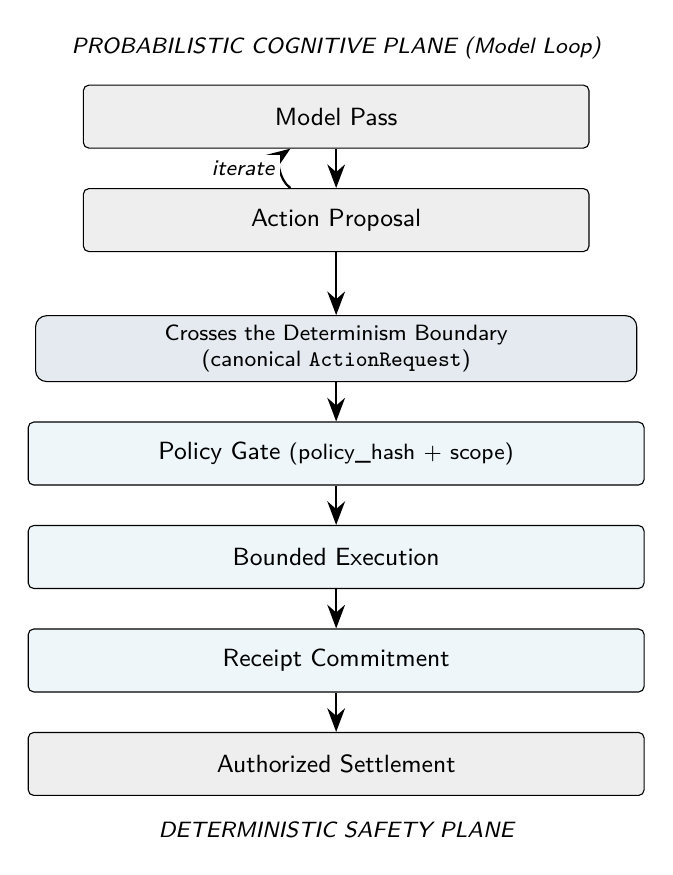
\begin{tikzpicture}[scale=1,transform shape,node distance=5mm and 10mm]
\node[font=\sffamily\footnotesize\itshape] (cl) {PROBABILISTIC COGNITIVE PLANE (Model Loop)};
\node[ioiplain,below=2mm of cl,text width=60mm] (mp){Model Pass};
\node[ioiplain,below=of mp,text width=60mm] (ap){Action Proposal};
\draw[ioiflow](mp)--(ap);
\draw[ioiflow](ap) to[bend left=55] node[ioilabel,left]{iterate} (mp);
\node[draw,fill=ioikw!12,rounded corners,below=8mm of ap,text width=74mm,align=center,font=\sffamily\footnotesize] (b){Crosses the Determinism Boundary\\(canonical \texttt{ActionRequest})};
\node[ioibox,below=5mm of b,text width=74mm] (pg){Policy Gate \footnotesize(policy\_hash + scope)};
\node[ioibox,below=of pg,text width=74mm] (ex){Bounded Execution};
\node[ioibox,below=of ex,text width=74mm] (rc){Receipt Commitment};
\node[ioiplain,below=of rc,text width=74mm] (st){Authorized Settlement};
\node[font=\sffamily\footnotesize\itshape,below=2mm of st] {DETERMINISTIC SAFETY PLANE};
\draw[ioiflow](ap)--(b);\draw[ioiflow](b)--(pg);\draw[ioiflow](pg)--(ex);\draw[ioiflow](ex)--(rc);\draw[ioiflow](rc)--(st);
\end{tikzpicture}
\end{center}

\textbf{Product domains are not runtime nodes by default.} A web app,
marketplace, or product surface may create runtime assignments, request
daemon-compatible execution, or project runtime state, but workers
execute inside local, hosted, decentralized, enterprise, TEE, or
customer-boundary runtime profiles.

A \textbf{managed worker instance} does not make aiagent.xyz the
execution runtime. aiagent.xyz resolves the worker package,
install/license rights, runtime profile, authority requirements,
subscription policy, and memory/archive policy. Execution occurs on a
daemon-compatible runtime node: local machine, hosted provider, DePIN
node, TEE, GPU job, browser sandbox, customer VPC, or enterprise/private
runtime.

Every execution node that performs IOI work runs, embeds, or speaks to a
daemon-compatible runtime profile. The Daemon decouples logical
isolation from physical hardware via a \textbf{Multi-Plane Scaling
Architecture}. The invariant is: regardless of deployment target, every
admitted path must preserve the declared authority, policy, envelope,
receipt, and Agentgres boundaries. Physical isolation, provider semantics,
capacity, privacy, attestation, and adapter control points vary and must not
be flattened into identical security claims.

Deployment examples: locally (Hypervisor), the planes may collapse into a
user-space virtualization layer over the host OS. On managed IOI or partner
provider infrastructure, they may scale horizontally across four distinct
planes, engaging public settlement only when an explicit trigger requires it:

Plane A: The Edge / Admission Plane

\begin{itemize}
\tightlist
\item
  \textbf{Role:} The stateless API and routing layer.
\item
  \textbf{Responsibilities:} Handles initial authentication, rate
  limiting, request normalization, routing, and session admission. It
  acts as the programmatic ingress for hosted \emph{ioi.ai} queries and
  third-party dApps.
\end{itemize}

Plane B: The Inference Plane

\begin{itemize}
\tightlist
\item
  \textbf{Role:} The cognitive engine.
\item
  \textbf{Responsibilities:} Horizontally scaled by model pool and queue
  depth. It handles fast reasoning, embeddings, and rerankers. It
  utilizes \emph{warm} capacity (Provider OSS or proprietary models) to
  eliminate cold starts for standard queries, while safely routing
  Bring-Your-Own-Key (BYOK) requests, where \emph{wallet.network}
  brokers BYOK keys and never exposes them to raw workflows.
\end{itemize}

Plane C: The Guest Workload Plane

\begin{itemize}
\tightlist
\item
  \textbf{Role:} The isolated environment where a model-backed worker,
  external harness, script, service module, or third-party binary
  attempts tool use. It is mediated away from provider-visible secrets,
  host authority, and the user's primary state by daemon policy,
  wallet.network leases, and Agentgres receipts.
\item
  \textbf{Responsibilities:} Horizontally scalable worker nodes that
  execute workflow steps, tool calls, browser/runtime jobs, and generate
  raw artifacts.
\item
  \textbf{Isolation:} Runs through declared execution lanes such as
  containers, namespaces, microVMs, WASM workloads, local tools, remote
  managed bridges, provider sessions, or cTEE/private-workspace paths. It
  boots in a zero-trust state. API calls cross daemon-governed mediation
  points such as adapter bridges, capability proxies, MCP gateways, or
  wallet.network leases, each enforcing the active authority envelope before
  effects are admitted.
\end{itemize}

Plane D: Hypervisor Daemon / Coordinator Plane (The Effect Boundary)

\begin{itemize}
\item
  \textbf{Role:} The bounded, capacity-governed execution-control role.
  This is the always-on daemon boundary that holds run state, policy
  bundles, tenant configurations, and cryptographic receipts while
  requesting decisions from local/domain policy and the applicable authority
  provider. wallet.network supplies portable delegated and designated
  high-risk authority paths; it is not required for every local act.
\item
  \textbf{Runtime Node Modes:} Execution venues that run Hypervisor
  daemon profiles.

  \begin{itemize}
  \tightlist
  \item
    \emph{Hosted IOI Runtime:} Hosted by the provider or
    provider-managed infrastructure for fast, consumer-facing tasks.
  \item
    \emph{Customer VPC Runtime:} Deployed directly inside a
    customer\textquotesingle s VPC or on-prem environment, allowing
    \emph{sas.xyz} to orchestrate tasks without exfiltrating enterprise
    data.
  \item
    \emph{Local Hypervisor:} Embedded inside Hypervisor on the
    user\textquotesingle s personal device.
  \item
    \emph{IOI Authority Gateway (Sidecar Profile):} Run locally or
    within customer boundaries to act as an external execution and
    policy boundary. Rather than serving as the primary interface, it
    runs as a background process ("sidecar") to intercept and normalize
    action requests from third-party cognitive environments, obtain the
    applicable policy and authority decision, and admit, deny, or mediate the
    resulting effect.
  \item
    \emph{Customer Boundary Runtime:} Deployed inside a customer VPC or
    on-prem environment so orchestration can occur without exfiltrating
    enterprise data.
  \item
    \emph{Hardware-Attested Confidential Runtime:} A TEE-backed runtime
    that may provide hardware attestation and memory-confidential
    execution under a vendor-specific threat model. Standard
    confidential VMs do not guarantee absolute protection against a
    compromised physical host. Vendor attestation, measured-boot evidence,
    cTEE, customer custody, and cryptographic operators provide different,
    non-interchangeable claims under their declared threat models. A TEE is
    one admissible private-execution substrate among several.
  \item
    \emph{Cryptographic Operator Runtime:} A proof-carrying runtime that
    uses FHE, MPC, ZK proofs, verifiable computation, or a hybrid
    construction to produce externally verifiable evidence without
    treating hardware attestation as the root of validity.
  \end{itemize}
\item
  \textbf{wallet.network guardian/access-point profile:} Operating within
  Hypervisor Core or the wallet.network authority path, a guardian/access-point profile
  may hold key shares, device attestations, approval state, or protected
  signing authority for a runtime. It does not by itself define protocol
  validity. Its signatures are accepted only when bound to canonical
  requests, policy hashes, monotonic sequence state, receipt obligations,
  wallet.network authority refs, and the applicable verifier
  requirements. Such a profile may integrate a minimal receipt sequencer
  (remote, local, or enclave-bound depending on the threat model) that
  maintains a persistent, monotonic counter (\emph{seq}) on disk to
  enforce an append-only, non-equivocating receipt chain.
\end{itemize}

\begin{longtable}[]{@{}>{\raggedright\arraybackslash}p{\linewidth}@{}}
\toprule\noalign{}
 \\
\midrule\noalign{}
\endhead
\bottomrule\noalign{}
\endlastfoot
\textbf{Safety Invariant:}\emph{\textbf{ }}Because the receipt
sequencer enforces monotonic sequence advancement on disk, equivocation
becomes detectable under the declared storage and runtime threat model.
A compromised host or execution worker cannot produce valid higher-tier
evidence unless it also satisfies the receipt-chain, verifier, and
challenge requirements for that action class. \\
\end{longtable}

\hypertarget{plane-enforced-isolation}{%
\subsubsection{2.2.1 Plane-Enforced
Isolation}\label{plane-enforced-isolation}}

For daemon-controlled workloads and capabilities, Plane C (where cognition
and guest work occur) is separated from Plane D (where the daemon evaluates
policy, requests applicable authority, and commits receipted state). Managed
I/O crosses the daemon effect boundary. Adapter profiles mediate only their
declared control points, so containment and interception claims must name the
actual substrate. When a brokered secret is required, wallet.network or an
approved authority client performs the capability or issues an operation-
scoped lease without exposing ambient secret material to the worker.

\hypertarget{deterministic-io-and-pinned-externalities}{%
\subsubsection{2.2.2 Deterministic IO and Pinned
Externalities}\label{deterministic-io-and-pinned-externalities}}

Pinned I/O is a versioned runtime-profile property, not a claim that IOI
eliminates all nondeterminism or intercepts every opaque external process. A
profile declares which externalities it mediates, how it binds them, and which
claims its receipts support:

\begin{itemize}
\tightlist
\item
  \textbf{Sequencing and time:} Replay-critical policy and authority checks use
  the sequence, expiry, revocation epoch, monotonic source, or trusted time
  source declared by their owner contract. Wall-clock observations may support
  UX and telemetry but do not become settlement truth merely by being logged.
\item
  \textbf{Network and tools:} A mediated call resolves through a
  RuntimeToolContract or surface MCP contract. The request, authority/policy
  decision, response commitment, artifacts, and normalized observation are
  covered by the applicable receipt profile.
\item
  \textbf{Randomness:} Any random selection relied upon for eligibility,
  challenge, routing, or settlement declares its source, bias assumptions,
  commitment/reveal or verifier method, and replay semantics. No universal VRF
  construction is fixed in this synthesis.
\item
  \textbf{UI and physical context:} A computer-use adapter may require
  application/window/DOM/visual target bindings and refuse a mismatch before
  action. The exact focus, freshness, and observation checks belong to the
  adapter contract; an unobserved UI surface is not claimed to be contained.
\end{itemize}

The invariant is coverage honesty: consequential effects crossing a declared
daemon or adapter boundary are canonicalized, gated, and receipted according
to that profile. Nondeterministic cognition, wall time, provider behavior, and
unmediated external state remain outside the proof unless a named evidence
source and verifier cover them.
The ``Run Anywhere'' Property

IOI's portability is achieved by separating kernel semantics from
workload packaging.

The \textbf{Hypervisor Daemon} and the underlying workload/kernel
substrate provide the execution invariant: they define how policies
bind, how receipts are formed, and how attestations are produced.

Workloads are packaged as \textbf{Universal Protocol Artifacts} (e.g.,
OCI images or equivalent bundles), allowing a workflow built locally on
a laptop to run on a cloud provider or committee node without changing its
portable contract. Transportability does not preserve every trust claim:
each environment declares its evidence and verifier profile, and receipts
advance only through the exact assurance ladder \texttt{attested},
\texttt{evidenced}, \texttt{verified}, \texttt{accepted},
\texttt{adjudicated}, and \texttt{settled}. A provider attestation, bond,
certificate, or public commitment may add evidence or recourse, but none
silently upgrades a receipt to a later stage.

\hypertarget{the-sidecar-deployment-profile-ioi-authority-gateway}{%
\subsubsection{2.2.3 The Sidecar Deployment Profile (IOI Authority
Gateway)}\label{the-sidecar-deployment-profile-ioi-authority-gateway}}

When running in sidecar compatibility mode, the \textbf{IOI Authority
Gateway} profile lets the Hypervisor Daemon operate as a deterministic,
policy-enforcing boundary for external, unaligned processes. In this
profile, the daemon does not own the external harness's cognitive loop
(the "thinking"). Instead, it mediates available control points and maps
proposed effects into Hypervisor proposals, gates, observations, and
receipts at host operating system, tool, and network boundaries.

This architecture implements the core thesis: \textbf{Models reason;
local/domain policy and the applicable authority provider authorize power;
the Hypervisor Daemon admits, enforces, and executes action.} wallet.network
is the portable delegated and designated high-risk authority profile, not the
source of every local decision.

A. Control Points and Interception Boundaries

Because external agent harnesses and editor/CLI/browser environments
(such as Cursor, Claude Code, Codex, OpenHands, Aider, DeepSeek-style
TUI harnesses, or proprietary hosted agents) expose only partial control
points, the Authority Gateway mediates the boundaries it can actually
observe through six deterministic control surfaces:

1. \textbf{Shell Commands:} The gateway intercepts terminal executions,
verifying package installations, file deletions, network sockets,
process spawns, and deployment commands against the active daemon policy
bundle.

2. \textbf{File System Watcher:} Monitors workspace diffs and git
configuration files. The gateway blocks unauthorized writes to protected
system directories or sensitive file extensions.

3. \textbf{Git Hook Mediation:} Enforces policies on branches,
force-pushes, and commit signing, automatically binding signed commit
hashes to corresponding execution receipts.

4. \textbf{Secret Isolation (wallet.network):} API keys and deployment
credentials remain within wallet.network vault custody. The gateway injects
temporary, operation-scoped credential leases at the network edge,
ensuring the raw secret material is never exposed to the
agent\textquotesingle s context window.

5. \textbf{Hypervisor MCP Gateway:} Exposes only the tools, surfaces,
sessions, automations, Foundry actions, and receipt/replay views selected by an
expiring or revocable gateway profile. Each call resolves to a declared
\textbf{RuntimeToolContract}, surface MCP contract, or operator-plane contract,
then crosses daemon admission and the applicable wallet.network authority path
before Agentgres records the result. A gateway profile is not a master key,
direct provider-credential broker, host-mutation bypass, or peer runtime.

6. \textbf{Context-Aware Approvals:} Requests a wallet.network step-up
approval gate when an external agent attempts an action exceeding
autonomous limits (e.g., spending capital, modifying production
environments).

\hypertarget{goal-kernel-and-typed-harness-broker}{%
\subsubsection{2.2.4 Goal Kernel, Outcome Rooms, and Typed Harness
Brokerage}\label{goal-kernel-and-typed-harness-broker}}

The \textbf{Goal Kernel} is the goal-shaped orchestration kernel used by
ioi.ai and Hypervisor Sessions. It turns normalized intent into a durable
\textbf{GoalRun}, executes a \textbf{GoalGroundingLoop}, selects a
\textbf{RoleTopology}, leases only the context and authority each role
needs, invokes compatible harnesses or workers, verifies results, and
reconciles receipts, memory proposals, skills, and continuation state. It is
not a super-agent, a swarm-control interface, or a runtime beside the daemon.

The Goal Kernel operates at the bounded-run scale. Persistent collective
pursuit sits one level above it in an \textbf{OutcomeRoom}. An OutcomeRoom
binds a durable objective to a \textbf{CollaborativeWorkGraph}: a governed
frontier of questions, hypotheses, tasks, review needs, verification needs,
resource needs, claims, attempts, findings, verifier challenges, admitted
outcome deltas, contribution lineage, budget, and replay. One room may contain
one or more GoalRuns, and a GoalRun may stand alone. Direct questions,
one-shot runs, ordinary automations, and single sessions do not acquire room
machinery merely because the substrate supports it.

Every persistent OutcomeRoom declares one shared-state ordering and admission
topology. Under \texttt{hosted\_admission}, one named governed domain orders
and admits room-level frontier, attempt, finding, evaluation, and decision
updates. Under \texttt{federated\_admission}, a versioned policy names the
participating domains, ordering or merge rules, quorum or adjudicator
requirements, conflict behavior, failover, recovery, and policy-version
transitions. Both modes preserve each party's local operational truth and
private context. A board, chat, inbox, digest, leaderboard, or replay is a
projection over admitted objects, never a universal mutable database or
authority source.

Each independent role works in a \textbf{ContextCell}. A
\textbf{ContextLease} bounds files, documentation, memory projections,
tools, connectors, budget, receipts, and authority. A typed
\textbf{ContextHandoff} moves a task brief, bounded result, finding, blocker,
test result, review request, verification result, resource request, decision
request, or continuation summary between cells. This preserves long-horizon
intent while preventing every actor from receiving a global context dump.

The harness broker boundary is:

\begin{center}
\textbf{TaskBriefPayload} $\rightarrow$ \textbf{HarnessInvocation}
$\rightarrow$ \textbf{HarnessAdapterEvent} $\rightarrow$
\textbf{WorkResult} / \textbf{OutcomeDelta} $\rightarrow$
\textbf{VerifierPath}.
\end{center}

\textbf{WorkResult} is the generic result seam for software, research,
ontology mutation, incident response, service delivery, physical missions,
review, evaluation, and custom work. \textbf{ImplementationResultPayload} is
only the software-implementation profile carrying changed-file, diff, test,
and implementation-summary fields. \textbf{OutcomeDelta} proposes an admitted
change to a frontier item, finding, ontology, state, capability, policy,
routing prior, or service outcome; producing a result never grants that change
admission by itself.

Open or cross-domain participation uses typed room contracts rather than raw
membership. \textbf{OutcomeRoomDiscovery} exposes a signed public or
permissioned objective and declared semantic, capability, eligibility,
privacy, budget, verifier, settlement, and contribution posture without
private room state. \textbf{RoomParticipationRequest} requests admission;
acceptance creates a bounded \textbf{RoomParticipantLease}. Resource and
capability offers, frontier items, work-claim leases, attempts, findings, and
verifier challenges remain proposals until the declared room admission path
accepts them. Retirement, expiry, quarantine, or revocation releases live
claims and may export a signed, policy-filtered
\textbf{ParticipantStateBundle}; it ends future access without erasing
permitted contribution, receipt, acceptance, settlement, or dispute lineage.

A HarnessProfile or Agent Harness Adapter may translate that contract into
provider-specific prompts, commands, RPC calls, or hosted-agent sessions, but
those renderings stay adapter-private. Durable coordination uses the typed
objects, receipts, artifacts, and Agentgres refs. Raw chat is never the
portable handoff or completion contract.

AIIP carries signed, sequenced, idempotent room updates and permitted refs
between sovereign domains. It does not execute attempts, own the
CollaborativeWorkGraph, or turn participant consensus into truth. Participant
input remains tainted until policy, isolation, verification, and the named
host or federation admission policy accept it. Multiple models, workers,
runtime nodes, providers, or keys controlled by one principal remain one party
when that principal controls authority, truth, verification, risk, or
settlement.

The daemon-owned \textbf{Agent Operating Plane} admits configured agents,
sessions, work queues, work items, WorkRuns, turn coordination, delegation,
conversation projections, usage, and execution/security telemetry. The
\textbf{Hypervisor Operator Plane} uses the same agent, model,
HarnessProfile, tool/MCP, authority, and receipt contracts to operate
Hypervisor itself; it is neither an ambient host administrator nor a
privileged child-session harness.

\hypertarget{the-anatomy-of-a-worker}{%
\subsection{2.3 The Anatomy of a Worker}\label{the-anatomy-of-a-worker}}

The IOI runtime decomposes agency into composable primitives rather than
treating each agent as a monolithic container. This decomposition serves
three purposes: deterministic execution boundaries, portability across
deployment targets, and intellectual property isolation between
participants.

The Worker Ontology

The IOI runtime decomposes agency into four distinct primitives:

\begin{enumerate}
\def\labelenumi{\arabic{enumi}.}
\tightlist
\item
  \textbf{Worker:} The core execution unit. Each worker has a defined
  role, a policy scope, a computational budget, and a capability set
  (defined by a canonical \emph{WorkerManifest}). Workers are actors,
  they do things.
\item
  \textbf{Model:} The cognitive backend. Models are cognitive backends,
  not peers to workers. The node owns the model routing and invocation
  boundaries. Model weights, local model files, local model servers, and
  provider endpoints are mounted by a \textbf{Model Deployment Profile},
  and are not part of the Hypervisor Node binary by default. The Model
  Deployment Profile MUST enforce the \emph{ModelWeightCustodyProfile}
  (see §2.3.1) to prevent accidental plaintext leakage of proprietary
  weights to hostile-root compute operators.
\item
  \textbf{Capability:} Capabilities are what workers use. This surface
  groups four pillars: 1. Connections (authenticated reach to external
  systems), 2. Computer Use (direct digital action, browser, desktop,
  terminal), 3. Skills (reusable, named operating patterns), and 4.
  Extensions (installable packages that grant new capabilities).
\item
  \textbf{Extension:} An installable package that grants new
  capabilities to a worker, extending its capability surface without
  modifying its core policy or identity.
\end{enumerate}

Model Routing vs. Worker Routing

IOI distinguishes \textbf{model routing} from \textbf{worker routing}.

\textbf{Model routing} selects an eligible cognition backend under
quality, privacy, authority, latency, context, commercial-rights, and
cost constraints. The route may use a direct provider API, managed or
dedicated endpoint, negotiated inference agreement, customer BYOK/BYOA,
a replaceable aggregator such as OpenRouter, or open/self-hosted weights.

\textbf{Worker routing} selects an accountable actor: a bounded worker
with a manifest, policy envelope, tools, runtime requirements, receipt
obligations, license terms, and settlement identity.

The canonical model-router API uses explicit runtime objects rather than
hardcoded provider names. A \textbf{ModelEndpoint} declares the provider
or local server, mount mode, deployment profile, model artifact ref,
auth mode, key ref, privacy class, supported model roles, architecture
profile, active-context strategy, and run-to-idle behavior. A
\textbf{ModelRoute} maps a role such as planner, executor, verifier,
summarizer, code, vision, embedding, or rerank to candidate endpoints
under cost, privacy, context, latency, route-rights, and fallback policy. A
\textbf{ModelInvocation} is the receiptable runtime act that invokes a
route with a task context, \emph{prim:model.invoke}, a
\emph{scope:model.invoke.*} authority scope, an authority grant, and a
receipt mode. \textbf{ModelDeploymentProfile} binds whether a route uses
bundled weights, local files, local servers, external APIs, dedicated
managed capacity, aggregator adapters, TEE sessions, DePIN sessions, or
customer VPCs.

Every unattended or customer-facing route resolves a versioned
\textbf{ModelRouteRightsContract}. It binds provider and model terms,
contract hash and validity window, endpoint and model version, access
mode, commercial posture, customer-facing and downstream rights,
automation and OEM/reseller authorization, credential principal,
provider allowlist, data collection, retention, region, price, required
parameters, fallback classes, and output-training right. Missing or
expired rights fail closed. A fallback that changes provider, model,
Worker, privacy posture, or commercial posture is a material semantic
substitution: it remains inside the declared constraint envelope, emits
routing evidence, and re-runs applicable verification and acceptance.

The lawful supply portfolio is intentionally plural:

\begin{enumerate}
\def\labelenumi{\arabic{enumi}.}
\tightlist
\item
  open or self-hosted weights where license, custody, quality, and
  operations permit;
\item
  direct provider APIs and managed endpoints for core routes and feature
  fidelity;
\item
  dedicated capacity or negotiated inference agreements for volume,
  service level, retention, residency, and data posture;
\item
  explicit OEM or reseller authorization when IOI exposes near-raw
  provider capability;
\item
  customer BYOK or BYOA for customer-owned cost and approved interactive
  harnesses; and
\item
  replaceable aggregators such as OpenRouter for bootstrap breadth,
  long-tail models, price and availability discovery, policy-qualified
  fallback, overflow, and experimentation.
\end{enumerate}

Named-user ChatGPT, Claude, or comparable chat/workspace subscriptions
are not production inference inventory. They may serve internal human
operators or an expressly provider-approved, user-scoped interactive
BYOA harness, but IOI must not pool, share, browser-automate, or resell
their limits as autonomous-worker capacity. An aggregator likewise does
not erase underlying provider terms, privacy posture, semantic
differences, or commercial rights, and use of an aggregator is not presumed
to authorize resale of near-raw model or API access. Inference permission
does not imply training, distillation, downstream resale, or OEM permission.

The execution-policy grammar is orthogonal to subscription plans:
\textbf{Auto / 1-of-N} selects the least-cost eligible route expected to
satisfy declared constraints and may run a verified cheap-first cascade;
\textbf{Pinned} uses the selected eligible route and fails closed unless
a qualified fallback was explicitly authorized; and \textbf{Compare /
N-of-N} runs declared attempts, preserves each admitted result, and
applies a named comparison, verifier, or synthesis rule.

BYOK provider keys belong in \textbf{wallet.network}. Runtimes receive
brokered authority grants or short-lived operation-scoped tokens, never
raw long-lived provider keys by default. Run-to-idle model serving is a
lifecycle primitive---\emph{cold -> warming -> ready -> busy -> draining
-> idle -> sleeping}---so local, hosted, DePIN, or customer-cloud model
routes can scale down without becoming invisible to policy, receipts, or
restore.

Mixture of Experts (MoE) is model routing. Federated Learning (FL) is
cooperative training. \textbf{Mixture of Workers (MoW) is accountable
labor routing.}

Mixture of Workers (MoW) is how autonomous labor is routed and executed.
The MoW worker economy is how autonomous labor is discovered, priced,
governed, and settled.

A Worker may internally use a dense model, an MoE model, a fine-tuned
local model, a tool-augmented model, a rules engine, a human approval
path, or a specialist trained, configured, or evaluated through
synthetic-data workflows. The protocol does not privilege the internal
substrate. It binds accountability to the Worker identity, manifest,
policy envelope, authority chain, evaluation receipts, contribution
receipts, and settlement surface. This preserves intellectual property
while ensuring that benchmarks, disputes, and royalties attach to the
verifiable actor rather than the opaque cognitive engine.

Node Packaging Principle

The Hypervisor Node contains model routing and invocation contracts; the
model itself is a mounted cognition backend unless a deployment profile
explicitly declares bundled weights. Bundled weights are allowed only
when declared by specific offline or local-only deployment profiles and
are not the architecture default. Service modules and workers invoke
models strictly through route aliases, never via direct file assumptions
or hardcoded provider names.

Instead, a "Worker" is decomposed into distinct, composable primitives.
This structure aligns with the Model Context Protocol (MCP) while
enforcing Hypervisor Daemon and IOI L0 security invariants.
It rigorously enforces the separation of \textbf{Logic} (Routing),
\textbf{Cognition} (Thinking), and \textbf{Execution} (Acting).


\begin{center}
\needspace{6\baselineskip}
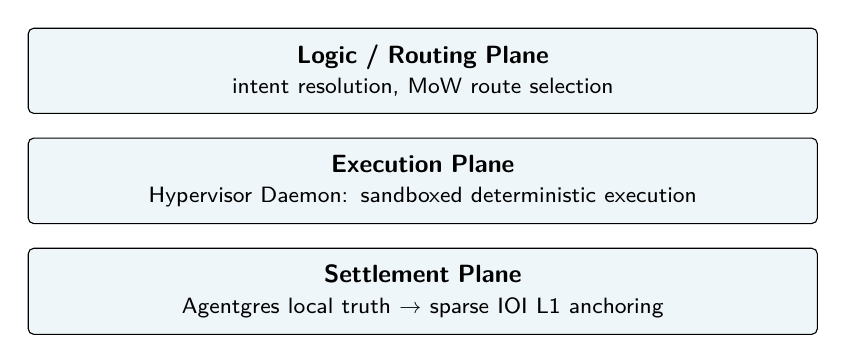
\begin{tikzpicture}[scale=1,transform shape,node distance=5mm and 10mm]
\node[ioibox,text width=96mm] (lg) {\textbf{Logic / Routing Plane}\\\footnotesize intent resolution, MoW route selection};
\node[ioibox,text width=96mm,below=3mm of lg] (ex) {\textbf{Execution Plane}\\\footnotesize Hypervisor Daemon: sandboxed deterministic execution};
\node[ioibox,text width=96mm,below=3mm of ex] (st) {\textbf{Settlement Plane}\\\footnotesize Agentgres local truth $\rightarrow$ sparse IOI L1 anchoring};
\end{tikzpicture}
\end{center}


1. The Agent Core (Logic, Cognition \& Context)

To reduce unnecessary exposure of developer IP while maintaining
zero-idle infrastructure, the agent's protected workspace intelligence
is never packaged as a single heavy asset. It is strictly decoupled into
three sub-components defined in the Worker Manifest:

\begin{itemize}
\tightlist
\item
  \textbf{The Logic Binary (WASM):} The state machine, prompt templates,
  tool wiring, and ReactFlow node configurations are compiled into a
  lightweight WebAssembly (WASM) binary (typically \textless5MB).
\item
  \emph{Distribution Boundary (WASM is not secrecy):} Compiling to WASM
  makes worker logic portable, typed, hashable, fuel-bounded, and easier
  to execute under daemon policy. It may slow casual inspection, but it
  is not a confidentiality primitive and must not be marketed as
  protection against determined reverse-engineering. Developer IP
  protection comes from not packaging private context, secrets, private
  retrieval state, proprietary weights, or authority as provider-readable
  plaintext, and from binding package use to manifests, policy,
  receipts, contribution accounting, and the selected execution/privacy
  posture.
\item
  \textbf{The Cognition Engine (Models \& Weights):} Logic binaries do
  not contain model weights; they declare cognition dependencies. Public
  foundational models may be fetched from public registries or caches.
  Proprietary models and private retrieval substrates are encrypted at
  rest and hydrated only under the action's declared
  \textbf{private-execution evidence profile}. Encryption-at-rest and a standard cTEE workspace
  wrap do not by themselves protect plaintext proprietary weights on a
  rented, hostile-root node: when both workspace privacy and proprietary
  weight secrecy are required on the same rented node, the execution
  path MUST pair cTEE with hardware confidential compute, or use the
  Cryptographic Operator path. Depending on the workload, the profile
  may require TEE attestation, FHE-backed private evaluation, MPC
  execution, ZK-proven model computation, deterministic replay evidence,
  or hybrid evidence. TEEs are admissible where ordinary software
  compatibility and performance matter. FHE/MPC/ZK-based execution is
  preferred where the action class requires stronger external
  verifiability or reduced dependence on hardware attestation roots. In
  all cases, the model or program hash, input commitments, output
  commitments, policy hash, leakage bounds, and verifier requirements
  are bound into the applicable \emph{CustodyProof}, proof refs, and
  receipt bundle. This reduces
  exposure under the declared substrate threat model and makes any
  authority-critical claim dependent on receipt completeness, not on
  trust in the execution venue.
\item
  \textbf{The Sovereign Context (The Data Moat):} For complex agents
  relying on public open-weights, the developer\textquotesingle s true
  IP is often their proprietary data. The agent\textquotesingle s
  knowledge base (e.g., 50,000 proprietary trading algorithms) is
  represented as encrypted semantic indexes and private memory refs in
  Agent Wiki / \emph{ioi-memory}, with durable mutations, policy refs,
  provenance, and artifact refs admitted through Agentgres. Even if the
  WASM logic is decompiled, without the decryption key, wallet.network
  authority, and authorized access to those memory projections and
  Agentgres-governed refs, the remote worker lacks the protected context
  that gives the workspace its operational advantage.
\end{itemize}

2. Tools (The Cognitive Interface / Intent)

\begin{itemize}
\tightlist
\item
  \textbf{Analogy:} OpenAI Function Definitions, MCP Resources \&
  Prompts.
\item
  \textbf{Definition:} The intent schema exposed to the Foundational
  Model or Cognition Engine.
\item
  \textbf{Role:} Allows the model to request an action.
\end{itemize}

\begin{longtable}[]{@{}>{\raggedright\arraybackslash}p{\linewidth}@{}}
\toprule\noalign{}
 \\
\midrule\noalign{}
\endhead
\bottomrule\noalign{}
\endlastfoot
\textbf{Invariant:}\emph{\textbf{ }}A Tool Call is a request, not an
execution grant. When a model selects a Tool, it generates a
\emph{ActionRequest} (derived from the MCP CallToolRequest standard).
This request is treated as untrusted input and MUST be validated by the
daemon effect boundary before any side effect occurs. \\
\end{longtable}

3. Drivers (The Execution Layer / MCP Servers)

\begin{itemize}
\item
  \textbf{Analogy:} Model Context Protocol (MCP) Servers, Hardware
  Drivers.
\item
  \textbf{Definition:} The binary or process that performs the I/O.
\item
  Architecture:

  \begin{itemize}
  \tightlist
  \item
    \textbf{Software Drivers (MCP Wrappers):} Standard MCP servers
    (e.g., \emph{stripe-mcp}, \emph{filesystem-mcp}) wrapped by the
    Hypervisor Daemon and bound by explicit \emph{RuntimeToolContract} schemas
    defining primitive capabilities and risk classes. The wrapper
    handles credential injection and policy enforcement transparently.
  \item
    \textbf{Native Drivers (Hypervisor Daemon):} Native code holding OS handles
    (e.g., Enigo for mouse control, xcap for screen capture). These
    provide the low-latency "Atomic Vision-Action Lock" required for
    GUI agents, which standard MCP over JSON-RPC cannot guarantee.
  \end{itemize}
\item
  \textbf{Role:} Executes the authorized I/O. Drivers do not "think";
  they obey the daemon.
\end{itemize}

\begin{longtable}[]{@{}>{\raggedright\arraybackslash}p{\linewidth}@{}}
\toprule\noalign{}
 \\
\midrule\noalign{}
\endhead
\bottomrule\noalign{}
\endlastfoot
\textbf{Invariant:}\emph{\textbf{ }}Drivers are Air-Gapped from the
Model. They never receive raw tokens or persistent API keys. They only
  receive policy-validated, canonical payloads from the Hypervisor Daemon,
injected with ephemeral credentials for the duration of a single
operation. \\
\end{longtable}

\hypertarget{model-weight-custody-and-routing-boundaries}{%
\subsubsection{2.3.1 Model Weight Custody and Routing
Boundaries}\label{model-weight-custody-and-routing-boundaries}}

To protect both developer IP and user privacy, the \textbf{Hypervisor}
enforces a strict separation between \textbf{Private Workspace
Protection} (governed by the cTEE) and \textbf{Proprietary Model-Weight
Protection} (governed by the Model Weight Custody Policy).

While the target cTEE posture is designed to keep a user's protected workspace
outside remote-host plaintext custody, it does not automatically
protect proprietary model weights. If a developer loads unencrypted,
proprietary weights directly into the memory (CPU/GPU) of a rented
remote node, a hostile host-root operator can copy those weights,
snapshot the disk, or inspect process memory.

To mitigate this risk, the Hypervisor requires that all worker
configurations declare their model access path in compliance with the
\emph{ModelWeightCustodyProfile}. In current model-router API terms this
is materialized as a \textbf{ModelWeightCustodyProfile} on the
deployment route. The profile is separate from
\textbf{ExecutionPrivacyPosture}: one answers what happens to the
weights; the other answers what happens to the user's workspace data.

\textbf{ModelWeightCustodyProfile lanes.}

\begin{longtable}[]{@{}
  >{\raggedright\arraybackslash}p{(\linewidth - 6\tabcolsep) * \real{0.2500}}
  >{\raggedright\arraybackslash}p{(\linewidth - 6\tabcolsep) * \real{0.2500}}
  >{\raggedright\arraybackslash}p{(\linewidth - 6\tabcolsep) * \real{0.2500}}
  >{\raggedright\arraybackslash}p{(\linewidth - 6\tabcolsep) * \real{0.2500}}@{}}
\toprule\noalign{}
& & & \\
\midrule\noalign{}
\endhead
\bottomrule\noalign{}
\endlastfoot
Lane & Weight custody claim & Valid use & Boundary \\
\textbf{public\_\allowbreak{}open\_\allowbreak{}weight} & Weights are public or intentionally
shareable. & Rented GPUs, DePIN nodes, local machines, hosted pools. &
Workspace privacy still depends on cTEE, redaction, local custody, or
another execution privacy posture. \\
\textbf{user\_\allowbreak{}local\_\allowbreak{}private\_\allowbreak{}weight} & Weights remain on
user-owned or customer-controlled machines. & Local/private model
serving, user-owned GPUs, enterprise clusters. & Strong weight custody
when the user's own authority domain controls the node. \\
\textbf{remote\_\allowbreak{}api\_\allowbreak{}private\_\allowbreak{}weight} & Provider keeps proprietary
weights behind an API; the user and rented compute node never mount
them. & Foundation-model APIs and managed private model services. &
Protects provider weights, but private user inputs cross a
provider-trust boundary unless redacted or declassified. \\
\textbf{provider\_\allowbreak{}trust\_\allowbreak{}remote\_\allowbreak{}mount} & User/org proprietary weights
are mounted on provider-visible infrastructure under contract or
accepted trust. & Explicit provider-trust deployments only. & Must not
be labeled private-native; requires disclosure, policy, and receipt. \\
\textbf{tee\_\allowbreak{}or\_\allowbreak{}customer\_\allowbreak{}cloud\_\allowbreak{}mount} & Proprietary weights mount
only inside an accepted hardware-confidential, customer-cloud, or
customer-controlled boundary. & Confidential GPU lanes, customer VPCs,
enterprise-controlled accounts. & Valid when attestation or customer
control satisfies policy; not a generic consumer-GPU claim. \\
\textbf{forbidden\_\allowbreak{}plaintext\_\allowbreak{}mount} & Requested mount would expose
non-public weights to an untrusted root provider. & Invalid route. &
Must be blocked unless policy changes to local/customer/API/TEE posture
or the owner explicitly accepts provider trust. \\
\end{longtable}

\textbf{Public trunk plus private head} is a composition pattern, not a
separate custody lane. The rented GPU may run public/open trunk weights
while the private head, scoring function, retrieval policy, or selection
logic remains local, wallet/guardian-bound, threshold-protected, or
cryptographic-operator-bound. This is the model-weight analogue of
Candidate-Lattice Private Decoding: keep high-throughput public kernels
on cheap compute while protected selection state stays outside provider
plaintext custody.

\hypertarget{the-determinism-boundary-invariant}{%
\subsection{2.4 The Determinism Boundary
(Invariant)}\label{the-determinism-boundary-invariant}}

As established in Section 1, IOI does not make AI
deterministic. It makes agentic state transitions deterministic by
enforcing the following invariants at the execution boundary.

The Determinism Boundary is the \emph{alignment-security boundary}. It
does not make inference deterministic. It determines when a proposed act
has enough canonical input, authority, policy binding, evidence, and
settlement context to become a consequential effect.

Implementation note: the current conformance docs do not treat
``Determinism Boundary'' as a separate runtime or contract family. They
realize it through CIRC semantic collapse, CEC admitted-effect collapse,
daemon gates, wallet.network authority, Agentgres admission, and
HarnessProfile adapter contracts.


\begin{center}
\needspace{6\baselineskip}
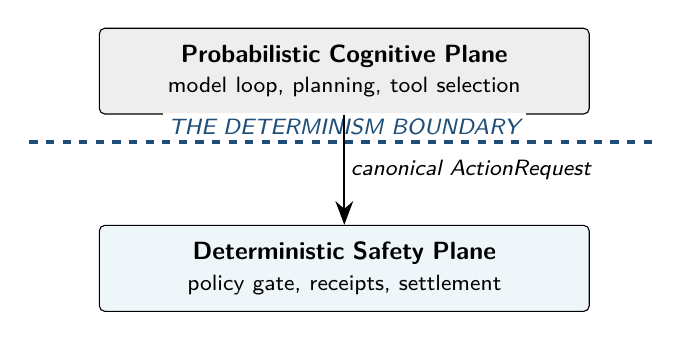
\begin{tikzpicture}[scale=1,transform shape,node distance=5mm and 10mm]
  % determinism boundary
\node[ioiplain,text width=58mm] (p) {\textbf{Probabilistic Cognitive Plane}\\\footnotesize model loop, planning, tool selection};
\node[ioibox,below=14mm of p,text width=58mm] (d) {\textbf{Deterministic Safety Plane}\\\footnotesize policy gate, receipts, settlement};
\draw[ioikw,very thick,dashed] ($(p.south)+(-4,-0.35)$) -- ($(p.south)+(4,-0.35)$) node[ioilabel,above,pos=0.5]{THE DETERMINISM BOUNDARY};
\draw[ioiflow] (p) -- node[ioilabel,right]{canonical ActionRequest} (d);
\end{tikzpicture}
\end{center}


The Determinism Boundary decouples \emph{Cognition} from \emph{Sanction}
and extends Own into Act. Models run on any hardware, embracing
hardware-induced drift. Strict mathematical determinism is enforced only
at the daemon effect boundary using integer-bound computation.

\textbf{Upstream (fuzzy):} Models may be stochastic, creative, and
adaptive.

\textbf{The Boundary:} Before any output can affect shared state
(payments, votes, property, credentials, durable records, irreversible
actions, or settlement), it must pass through a strict, normative
invariant set. This is the consequential boundary of Web4 Act.

\textbf{Downstream (rigid):} The resulting artifact (Receipt →
Commitment → Certificate/Resolution) is immutable, machine-verifiable,
and enforceable.

The Determinism Boundary Invariant Set (DBIS)

To ensure skeptics, auditors, and protocol engineers can mathematically
verify the execution boundary, the Hypervisor Daemon enforces the following
normative invariants:

\hfill\break

\begin{longtable}[]{@{}>{\raggedright\arraybackslash}p{\linewidth}@{}}
\toprule\noalign{}
 \\
\midrule\noalign{}
\endhead
\bottomrule\noalign{}
\endlastfoot
\textbf{DBIS-1: Canonicalize-before-hash/sign (MUST, Fail-Closed):}All
\emph{ActionRequest} objects and any commitment material MUST be
canonicalized via RFC 8785 (JSON Canonicalization Scheme) prior to
hashing (e.g., \emph{try\_hash()}) or signing. This prevents
cross-runtime mismatch and ensures hashes are stable. Failure to
canonicalize MUST result in the request being dropped. \\
\end{longtable}

\begin{longtable}[]{@{}
  >{\raggedright\arraybackslash}p{(\columnwidth - 0\tabcolsep) * \real{1.0000}}@{}}
\toprule\noalign{}
 \\
\midrule\noalign{}
\endhead
\bottomrule\noalign{}
\endlastfoot
DBIS-2: Tiered Safety Decision Determinism:

\begin{itemize}
\tightlist
\item
  \textbf{DBIS-2A Deterministic Safety (MUST):} Any decision that
  changes the \emph{Allow / Block / Require Approval} semantics for
  high-risk actions MUST be computed via a deterministic mechanism
  (e.g., a pinned deterministic inspection profile running in a strict
  WASM sandbox).
\item
  \textbf{DBIS-2B Advisory Safety (MAY):} Non-deterministic models
  (e.g., standard LLMs) MAY be used for heuristic hints, intent parsing,
  or assistive transforms \textbf{only if} the final enforceable
  decision remains fully DBIS-2A compliant.
\end{itemize} \\
\end{longtable}

\begin{longtable}[]{@{}
  >{\raggedright\arraybackslash}p{(\columnwidth - 0\tabcolsep) * \real{1.0000}}@{}}
\toprule\noalign{}
 \\
\midrule\noalign{}
\endhead
\bottomrule\noalign{}
\endlastfoot
DBIS-3: Explicit and Scoped Pinned Externalities (MUST):

Externalities relevant to execution MUST be deterministically bound. For
example, \emph{window\_id} and visual perceptual hashes are explicitly
pinned for UI and browsing actions. However, \textbf{wall-clock
timestamps} (e.g., \emph{SystemTime::now()}) are explicitly classified
as \textbf{non-binding telemetry} unless sourced directly from a
verified chain/block timestamp. \\
\end{longtable}

\begin{longtable}[]{@{}
  >{\raggedright\arraybackslash}p{(\columnwidth - 0\tabcolsep) * \real{1.0000}}@{}}
\toprule\noalign{}
 \\
\midrule\noalign{}
\endhead
\bottomrule\noalign{}
\endlastfoot
DBIS-4: The Deterministic Retry Contract (SHOULD):

Agents inherently fail and retry. Retries are permitted, but they MUST
be deterministic, bounded, and fully recorded. A failed execution MUST
generate a failure receipt, increment a deterministic attempt counter
against a strict budget, and be included in the verification evidence.
Unbounded, unlogged heuristic loops are strictly prohibited. \\
\end{longtable}

\begin{longtable}[]{@{}
  >{\raggedright\arraybackslash}p{(\columnwidth - 0\tabcolsep) * \real{1.0000}}@{}}
\toprule\noalign{}
 \\
\midrule\noalign{}
\endhead
\bottomrule\noalign{}
\endlastfoot
DBIS-5: Binding Set for Enforceability Artifacts (MUST)

For any consequential action that crosses the boundary, the runtime MUST
emit a transaction-shaped action/evidence record that securely binds:

\begin{enumerate}
\def\labelenumi{\arabic{enumi}.}
\tightlist
\item
  \emph{request\_hash} (The canonical intent)
\item
  \emph{policy\_hash} (The ruleset governing the action)
\item
  Context bindings where relevant (e.g., \emph{window\_id})
\item
  Approval references (if the action required a user step-up token)
\end{enumerate} \\
\end{longtable}

Enforceable vs. Observational Artifacts

To prevent verification bloat and preempt disputes over
non-deterministic telemetry (such as local machine latency), the
determinism boundary strictly categorizes all outputs into two artifact
classes:

\begin{itemize}
\tightlist
\item
  \textbf{Enforceability Artifacts (Settlement-Grade):} These are the
  inputs to disputes and economic liability. This includes
  \emph{ActionProposal} records, \emph{GateResult} receipt refs, settlement
  commits, and Merkle inclusion proofs. They are not Web2-style logs;
  they are transaction records for acts that may become economically or
  legally consequential. These rely exclusively on deterministic inputs,
  bounded states, and cryptographic signatures.
\item
  \textbf{Observational Artifacts (Telemetry):} These are local UI and
  ops events (e.g., \emph{WorkloadReceiptEvent} streams, wall-clock
  timestamps, local activity feeds). While useful for user experience
  and debugging, they contain non-deterministic metadata and
  \textbf{MUST NOT} be used to evaluate policy compliance or settle
  on-chain disputes.
\end{itemize}

\begin{longtable}[]{@{}
  >{\raggedright\arraybackslash}p{(\columnwidth - 0\tabcolsep) * \real{1.0000}}@{}}
\toprule\noalign{}
 \\
\midrule\noalign{}
\endhead
\bottomrule\noalign{}
\endlastfoot
Design Principle (Normative):

IOI constrains the \emph{effects }of intelligence, not the
\emph{process} of intelligence. That is how Web4 turns Own into Act
without trying to make cognition itself deterministic. \\
\end{longtable}

\hypertarget{the-intent-contract-schema-ics}{%
\subsubsection{2.4.1 Typed Intent, Constraints, and Acceptance
Contract}\label{the-intent-contract-schema-ics}}

To enable replay, verification, delivery review, and optional dispute
resolution, a GoalRun or task binds normalized intent to typed constraints,
acceptance criteria, verifier paths, budgets, policy/authority requirements,
and output contracts. Concrete carriers include GoalRun, TaskBriefPayload,
ActionProposal, workflow step contracts, ServiceOrder terms, and domain
schemas; there is no separate universal intent-contract object in current
canon.

The typed contract makes an act transaction-shaped by converting the
relevant parts of natural-language intent into fields, constraints,
acceptance, and evidence criteria that can be signed, replayed, verified,
challenged, delivered, or settled when applicable.

\hypertarget{the-adversarial-hierarchy-adaptive-work-graphs-deterministic-gate}{%
\subsubsection{2.4.2 The Adversarial Hierarchy (Adaptive Work Graphs /
Deterministic
Gate)}\label{the-adversarial-hierarchy-adaptive-work-graphs-deterministic-gate}}

To support massive, high-velocity agent work graphs without exposing the
Hypervisor Node to chaotic or malicious state changes, IOI bifurcates
execution into two distinct security zones. This architecture treats the
Hypervisor Node's protected context (files, wallet, calendar, memory,
and authority state) as \textbf{protected workspace/domain state}, and
all agent activities as \textbf{Proposed State Deltas}.


\begin{center}
\needspace{6\baselineskip}
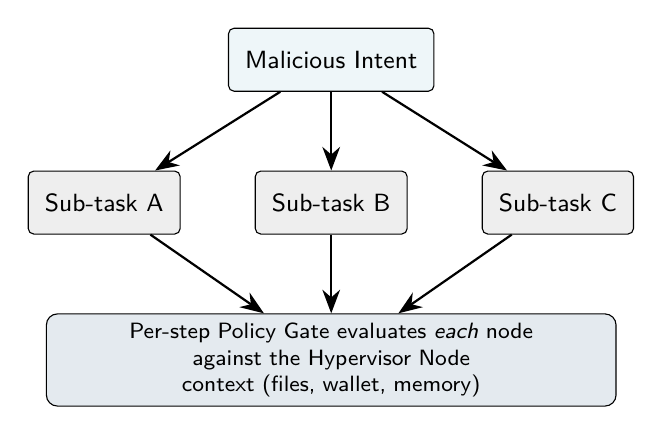
\begin{tikzpicture}[scale=1,transform shape,node distance=5mm and 10mm]
 % adversarial work graph
\node[ioibox] (r){Malicious Intent};
\node[ioiplain,below left=10mm and 6mm of r] (a){Sub-task A};
\node[ioiplain,below=10mm of r] (b){Sub-task B};
\node[ioiplain,below right=10mm and 6mm of r] (c){Sub-task C};
\node[draw,fill=ioikw!12,rounded corners,below=10mm of b,text width=70mm,align=center,font=\sffamily\footnotesize] (g){Per-step Policy Gate evaluates \emph{each} node\\ against the Hypervisor Node context (files, wallet, memory)};
\draw[ioiflow](r)--(a);\draw[ioiflow](r)--(b);\draw[ioiflow](r)--(c);
\draw[ioiflow](a)--(g);\draw[ioiflow](b)--(g);\draw[ioiflow](c)--(g);
\end{tikzpicture}
\end{center}


The Hypervisor Daemon enforces an \textbf{Adversarial Hierarchy}:

Zone A: The Optimistic Internal Zone (The Delegated Work Graph)

Execution occurs within a \textbf{Delegation Thread}. Workers operate
with high velocity using \textbf{Advisory Peer Review}. When a Worker
proposes a change (a "State Delta"), another Worker in the graph MAY act
as a reviewer to flag obvious errors. Trust is \textbf{Optimistic}:
state transitions in this zone are provisional (labeled as speculative
state). They allow for messy, non-linear collaboration (e.g., hundreds
of asynchronous drafts or plans) but \textbf{MUST NOT} affect the User
Node's protected workspace/domain state.

Zone B: The Deterministic Egress Gate (Daemon/Owner Boundary)

The boundary between the Graph\textquotesingle s provisional state and
the User\textquotesingle s protected state is the daemon effect boundary
and owner/authority checkpoint. This is an authoritative, local-first
checkpoint. No effect lands in the protected workspace context without
passing this gate.

The Gate executes a \textbf{Deterministic Gate VM}- a canonical,
sandboxed verification runtime that validates two vectors:

\begin{enumerate}
\def\labelenumi{\arabic{enumi}.}
\tightlist
\item
  \textbf{State Validity:} It executes a \textbf{Validation Recipe} to
  verify the output (e.g., "Do the unit tests pass?", "Are the facts
  verified against authoritative evidence refs?", "Is the transaction
  syntax valid?").
\item
  \textbf{Policy Compliance:} An \textbf{Intent Contract Evaluator}
  verifies the \textbf{Provenance Ledger}, ensuring the State Delta came
  from a hired worker, the chain of custody is intact, and the effect
  does not violate authorized \emph{prim:*} and \emph{scope:*}
  restrictions.
\end{enumerate}

Only if all checks pass does the gate emit the applicable \textbf{GateResult},
\textbf{ExecutionResult}, and receipt refs and admit the resulting state
transition under the owner contract.

\hypertarget{fractal-edge-in-topology-and-the-l0l1-boundary}{%
\subsection{2.5 Fractal Edge-In Topology and the L0/L1
Boundary}\label{fractal-edge-in-topology-and-the-l0l1-boundary}}

IOI\textquotesingle s fractal topology routes state transitions and
settlements across strict boundaries:

Governed Autonomous-System Chain

\emph{- Accepts local module invocations, proposals, receipts,}

\emph{and state transitions}

\emph{\textbar{}}

\emph{v (Local Settlement)}

Hypervisor Node (Local Settlement Domain)

\emph{- Coordinates multiple autonomous-system chains}

\emph{- Settles local interop, authority outcomes, local receipt-roots}

\emph{\textbar{}}

\emph{v (Global Anchoring \& Escalation)}

IOI L1 (Global Settlement Layer)

\emph{- Anchors selected roots (node, system-chain, policy,}

\emph{module, upgrade roots)}

\emph{- Settles public rights, disputes, reputation, registry,
economics}

The layers are not identical. They reuse the same kernel doctrine at
different authority and commitment boundaries.

The \textbf{IOI kernel / L0 substrate} provides reusable machinery for:
domain creation; policy namespaces; Agentgres domain state; runtime-node
profiles; worker and service manifests; receipt and artifact semantics;
routing and settlement mirrors; upgrade and governance hooks; and L1
commitment interfaces.

\textbf{IOI L1} provides: public registry roots; identity and rights
anchors; escrow and fee routing; dispute bonds; settlement finality;
governance and upgrade approvals; and sparse public commitments.

The topology is \textbf{edge-in}. Runtime edges execute; domain kernels
remember; IOI L1 settles.

The purpose of this topology is composability. A result may involve one
user's local Hypervisor, a managed worker from \emph{aiagent.xyz}, data
recipes from a domain ontology, a hosted model, a verifier worker, a
\emph{sas.xyz} service workspace, and an IOI L1 escrow. The architecture
must let those layers compose without becoming one centralized runtime.

\hypertarget{the-three-execution-axes}{%
\subsubsection{2.5.1 The Three Execution
Axes}\label{the-three-execution-axes}}

Rather than hardcoding static "lanes," the IOI runtime evaluates
execution along three dynamic axes, which the user or developer
configures as execution "presets."

Axis 1: Where it runs (The Physical Target)

\begin{itemize}
\tightlist
\item
  \textbf{Local Hypervisor:} Execution occurs on the
  user\textquotesingle s personal device. Ideal for tasks requiring
  local GPU, direct desktop/browser control, or ultimate sovereignty
  where no hosted dependency is desired.
\item
  \textbf{Customer Boundary (VPC / On-Prem):} Execution occurs within an
  enterprise\textquotesingle s secure firewall. A Boundary Coordinator
  orchestrates tasks, ensuring that proprietary data never leaves the
  internal network.
\item
  \textbf{Provider-Hosted:} Execution occurs on a remote cloud or DePIN
  provider. Ideal for batch jobs, heavy inference requiring massive
  hardware, or proprietary models that cannot be distributed locally.
\item
  \textbf{Decentralized Private Execution:} Decentralized compute nodes
  with minimized task capsules whose substrate-specific exposure bounds
  are bound into private-execution receipts; suited to third-party
  execution of sensitive workloads where centralized infrastructure is
  undesirable.
\item
  \textbf{Hardware-Attested Confidential:} Attested confidential compute
  nodes (e.g., AWS Nitro, Google Confidential Space) providing
  hardware-bounded execution and remote attestation under a
  vendor-specific threat model. Hardware-attested TEEs (such as SGX or
  confidential GPUs) are an optional performance profile, not the
  baseline definition of cTEE: the baseline cTEE model relies on
  software-driven cryptographic containment --- candidate lattices,
  cryptographic operators, and plaintext-free mounts --- treating
  hardware attestation as one admissible private-execution substrate among
  several.
\end{itemize}

Axis 2: How inference is sourced and commercially admitted

\begin{itemize}
\tightlist
\item
  \textbf{Open / Self-Hosted Model:} Licensed weights run locally, in the
  customer's infrastructure, or on an admitted managed runtime with
  explicit custody and attestation posture.
\item
  \textbf{Bring Your Own Key or Account (BYOK/BYOA):} The customer binds
  an external API credential or expressly permitted interactive account
  through wallet.network. The customer owns supplier cost; IOI may
  separately price conductor, runtime, governance, support, or audit
  value.
\item
  \textbf{Direct or Dedicated Provider Route:} IOI or the customer uses
  a provider API, managed endpoint, reserved capacity, or negotiated
  inference agreement under a versioned route-rights contract.
\item
  \textbf{Aggregator Route:} A replaceable adapter such as OpenRouter
  supplies breadth, overflow, discovery, or policy-qualified fallback;
  the underlying provider, terms, privacy posture, and price remain
  visible and eligible under the route-rights contract.
\item
  \textbf{Proprietary or Specialized Model:} Closed or custom weights run
  behind an admitted provider, dedicated endpoint, customer boundary, or
  confidential-compute profile under explicit inference and downstream
  rights.
\end{itemize}

Named-human workspace seats are excluded from pooled managed-worker
supply unless a signed provider agreement authorizes the exact use.

Axis 3: Privacy and Evidence Posture

Privacy posture and evidence posture are related but distinct. The runtime
records technical states such as \emph{private\_native},
\emph{redacted\_api}, \emph{provider\_trust}, and \emph{unsafe}; those
states are admission evidence, not separate product modes. Hardware TEEs,
cTEE/private workspaces, local/customer boundaries, FHE, MPC, ZK proofs,
verifiable computation, and deterministic replay may satisfy different
parts of a required receipt profile. \textbf{Verified} means that the declared
verifier has accepted the covered evidence and boundary claim; it does not
name a single substrate, imply outcome acceptance or settlement, or turn an
unsafe custody route into a private one.

\hypertarget{the-derived-presets-lanes}{%
\subsubsection{2.5.2 Managed Execution Modes}\label{the-derived-presets-lanes}}

The user-facing managed execution selector has exactly two modes. Speed,
model choice, provider choice, and evidence strength remain separate
controls:

\begin{itemize}
\tightlist
\item
  \textbf{Standard:} IOI-managed execution is private-native at the
  operating-substrate layer by default: cTEE / Plaintext-Free Runtime
  Mounting, scoped authority, connector vaulting, and receipts are baseline
  discipline. A disclosed provider-trust model route may still receive
  sensitive plaintext when policy permits; that boundary must be visible in
  the execution privacy posture and receipts.
\item
  \textbf{Private:} Adds a no-provider-trust model route for protected
  data through open-weight or user-controlled models in a local, BYO
  private-node, customer-boundary/customer-cloud, cTEE, hardware-TEE, or
  other custody-proven route. The stronger promise must be supported by
  custody proof, model/API boundary evidence, and receipts.
\end{itemize}

Private mode may be a paid managed posture when IOI provisions stricter
runtime custody, protected connector processing, encrypted storage,
attestation/custody proof, audit/replay, or persistent background work.
Connecting an app, granting ordinary authority, or using local/BYOM/BYOA
without IOI-managed private compute is not by itself a connector tax.

\hypertarget{agentgres-the-per-domain-state-substrate}{%
\subsubsection{2.5.3 Agentgres: The Per-Domain State
Substrate}\label{agentgres-the-per-domain-state-substrate}}

Agentgres is the per-domain state substrate. It stores operational
truth, not IOI L1 economic settlement. Every consequential Web4
application domain (e.g., \emph{aiagent.xyz}, \emph{sas.xyz}, enterprise
deployments) runs its own kernel/runtime deployment with its own
Agentgres domain.

Agentgres is not a thin index over Filecoin/CAS blobs. It owns the
canonical operation log, object heads, constraints, indexes,
projections, subscriptions, delivery state, and quality/contribution
ledgers. The IOI L1 blockchain is used strictly for sparse root
commitments, contract state, and dispute resolution. Truth is anchored
in Agentgres canonical operations and deterministic object state, not in
mutable table rows.

\hypertarget{the-eject-bridge-pointer-based-state-injection}{%
\subsubsection{2.5.4 The "Eject" Bridge: Pointer-Based State
Injection}\label{the-eject-bridge-pointer-based-state-injection}}

Because all engines and execution targets share the exact same Artifact
Schema and Fractal Query Fabric (FQF) standards, a user can seamlessly
migrate an agent from Local (Private) to Network (Public). This is not a
bulk data upload, but a State Injection via the \emph{ai://} global
namespace. To prevent blockchain bloat, the protocol enforces a strict
separation between Logic (Storage) and Authority (Chain).

The Migration Protocol executes in three atomic steps:

1. Content Addressing (The Store):

The Hypervisor freezes the local agent. It uploads the static payload
bytes (WASM binary, React UI bundle, connector schemas) to the selected
storage backend (a decentralized network such as IPFS/Filecoin, or an
enterprise/local CAS), which holds them as opaque blobs. The
corresponding \emph{ArtifactRef}s are declared, versioned, and evaluated
exclusively inside the Agentgres Artifact Plane.

\begin{itemize}
\tightlist
\item
  \emph{Result:} A set of Content Identifiers (CIDs).
\end{itemize}

2. Root Anchoring (The Transaction):

Most portability stays local: the canonical record is the Agentgres
\emph{ArtifactRef}/\emph{PayloadRef}. When---and only when---a public
registry listing, marketplace publication, or cross-domain settlement is
triggered, the user submits a \emph{DeployAgent} transaction to the IOI
L1. That L1 payload is minimal (approx. 200 bytes); it contains only the
pointers:

\begin{itemize}
\tightlist
\item
  \textbf{Identity:}
  \emph{ai://\textless authority\textgreater/\textless agent\_id\textgreater/\textless version\textgreater{}}
  (The human-readable DNS name).
\item
  \textbf{Logic Root:} \emph{ManifestCID} (Pointer to the code).
\item
  \textbf{State Root:} \emph{agentgres\_projection\_watermark} (The
  Agentgres projection anchor) or \emph{StateRoot}.
\end{itemize}

3. Hydration (The Execution):

A provider environment picks up the job. It uses the
\emph{ManifestCID} to pull the logic, and the \emph{StateRoot} to
rebuild the required projections or retrieve the context slice required
for execution.\\

\begin{longtable}[]{@{}>{\raggedright\arraybackslash}p{\linewidth}@{}}
\toprule\noalign{}
 \\
\midrule\noalign{}
\endhead
\bottomrule\noalign{}
\endlastfoot
\textbf{Zero-Bloat Invariant:}\emph{\textbf{ }}A future IOI Mainnet
stores selected commitments, not payload bytes. It may
anchor publisher identity, registry commitments, valid state roots, and
settlement/dispute facts when triggered. The gigabytes of UI bundles,
vector-memory archives, datasets, packages, and model payloads are
retrieved from storage backends only by the runtime or provider lane
provisioning the workload, under Agentgres ArtifactRef/PayloadRef meaning,
wallet.network authority, and any declared \textbf{ModelWeightCustodyProfile}. \\
\end{longtable}

Zero-bloat is not zero-retention. For every challenge-eligible
commitment, the corresponding Agentgres ArtifactRefs and PayloadRefs
MUST declare a \emph{challenge\_epoch\_ref}, a \emph{retention\_until}
height or time, and one or more retrievability lanes (local archive,
provider archive, Filecoin/IPFS/S3-style object store, or
Witness-Coded Recovery Capsule). The declared retrievability window MUST
strictly dominate the challenge period plus publication and retrieval
slack:

\[
T_{\mathrm{retain}} \geq
T_{\mathrm{challenge}} + \Delta_{\mathrm{publish}} +
\Delta_{\mathrm{retrieve}} + \Delta_{\mathrm{verify}}.
\]

If a challenged payload cannot be served, reconstructed, and hash-verified
inside its declared challenge epoch, that absence is itself objective
evidence. The dispute path fails closed: irreversible release is halted
and the missing-evidence dispute resolves in favor of the challenger
unless the respondent produces the required bytes or a valid recovery
bundle before the epoch closes.

\hypertarget{node-profiles-and-hypervisoros}{%
\subsubsection{2.5.5 Node Profiles and
HypervisorOS}\label{node-profiles-and-hypervisoros}}

Execution venues across the network are classified into standardized
\textbf{Runtime Node Profiles}. To ensure bare-metal operational
integrity and reproducible environments, high-performance nodes can
deploy \textbf{HypervisorOS} --- a minimal, measured operating-system
image where the \textbf{Hypervisor Daemon} operates as the daemon-root
node process.

HypervisorOS is the \textbf{Type 1} substrate posture of the same
Hypervisor control plane. \textbf{Type 2} is Hypervisor Desktop /
Workstation hosted on a normal operating system and governing local VMs,
sandboxes, models, tools, agents, connectors, and environments.
\textbf{Type 3} is the autonomy posture across sessions, WorkRuns,
workers, harnesses, model routes, tools, authority, receipts, replay,
outcomes, and promotion. These are not three products. Type 1 and Type 2
provide the inspectable substrate; Type 3 virtualizes governed autonomy
above it. HypervisorOS improves control, integrity, containment,
measurement, and reproducibility, but it never replaces cTEE
no-plaintext-custody or an applicable confidential-compute proof.

\textbf{Implementation status.} HypervisorOS is a planned node profile; no
current HypervisorOS image or measured-boot product build is claimed.

The target boot flow generates a signed
\textbf{HypervisorOSBootReceipt} based on a
\textbf{HypervisorOSBootProfile} and declared hardware measurements. This
receipt is bound
to the node's \textbf{node capability manifest}, detailing its physical
resources (such as VRAM, CPU cores, and network capability) and recording
the measured image under the profile's attestation assumptions.


\begin{center}
\needspace{6\baselineskip}
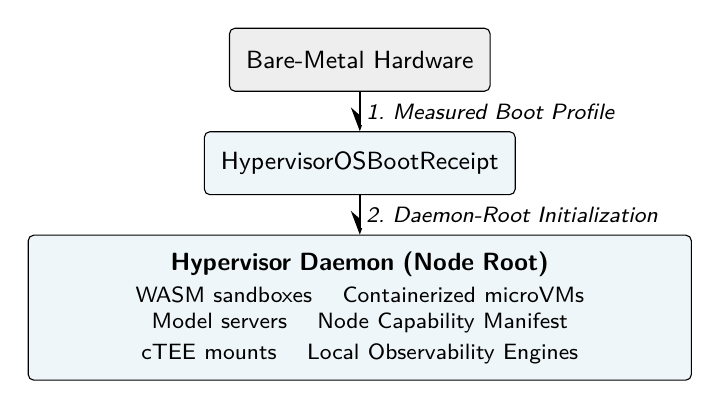
\begin{tikzpicture}[scale=1,transform shape,node distance=5mm and 9mm]
\node[ioiplain] (hw) {Bare-Metal Hardware};
\node[ioibox, below=of hw] (br) {HypervisorOSBootReceipt};
\node[ioibox, below=of br, text width=80mm] (dae) {\textbf{Hypervisor Daemon (Node Root)}\\[2pt]
\footnotesize WASM sandboxes \quad Containerized microVMs\\
\footnotesize Model servers \quad Node Capability Manifest\\
\footnotesize cTEE mounts \quad Local Observability Engines};
\draw[ioiflow] (hw) -- node[ioilabel,right]{1.\ Measured Boot Profile} (br);
\draw[ioiflow] (br) -- node[ioilabel,right]{2.\ Daemon-Root Initialization} (dae);
\end{tikzpicture}
\end{center}

While HypervisorOS provides excellent node measurement, operational
control, and execution reproducibility, \textbf{it is not a privacy
cure-all.} If a node is deployed on rented hardware where a malicious
provider retains physical or out-of-band management access, the provider
can still read plaintext state from CPU registers or GPU memory if it is
mounted without encryption.

Therefore, a signed boot receipt or measured boot sequence is operational
integrity evidence under its threat model, not a substitute for
software-level cTEE candidate-lattice decoding or hardware-level
confidential GPU protections.

\textbf{Runtime node profiles.}

\begin{longtable}[]{@{}
  >{\raggedright\arraybackslash}p{(\linewidth - 8\tabcolsep) * \real{0.2000}}
  >{\raggedright\arraybackslash}p{(\linewidth - 8\tabcolsep) * \real{0.2000}}
  >{\raggedright\arraybackslash}p{(\linewidth - 8\tabcolsep) * \real{0.2000}}
  >{\raggedright\arraybackslash}p{(\linewidth - 8\tabcolsep) * \real{0.2000}}
  >{\raggedright\arraybackslash}p{(\linewidth - 8\tabcolsep) * \real{0.2000}}@{}}
\toprule\noalign{}
& & & & \\
\midrule\noalign{}
\endhead
\bottomrule\noalign{}
\endlastfoot
Node Profile & Host / Hardware Ownership & Target Execution Environment
& Isolation / Privacy Posture & Primary Use Case \\
\textbf{Local} & User-owned (personal computer). & Standard user-space
hypervisor layer. & High (no external network data leakage). & Daily
personal assistance, document summary, local code synthesis. \\
\textbf{Workstation} & User/team-owned (high-perf local rig). & Direct
OS process within a local VM. & High (sovereign local hardware control).
& High-throughput local model inference and development. \\
\textbf{Hosted} & Third-party provider (SaaS / cloud VM). & Rented
virtual machine (non-attested). & Low (host-root can inspect VM memory).
& Generic low-risk API agents and standard web scrapers. \\
\textbf{VPC} & Customer VPC (enterprise cloud). & Controlled enterprise
subnet and VM instances. & Medium (bound to enterprise security policy).
& Internal enterprise workflows and sensitive database queries. \\
\textbf{DePIN} & Untrusted rented provider. & Docker container or
ephemeral VM. & Low (host can read plaintext); requires cTEE. &
Cost-optimized, scale-out compute pipelines. \\
\textbf{TEE / Confidential GPU} & Attested cloud hardware (AMD SEV,
NVIDIA CC). & Attested secure VM enclave / confidential memory. & High
(hardware-enforced memory isolation). & Proprietary weight mounting and
highly sensitive financial computation. \\
\textbf{Enterprise} & Dedicated on-prem server. & On-premises hardware
behind a strict corporate firewall. & High (completely internal state
retention). & Sovereign corporate operations and internal compliance
systems. \\
\textbf{HypervisorOS} & Dedicated server / bare-metal. & Minimal,
measured-boot bare-metal image. & High (system integrity); Low (physical
hardware spying still possible). & Core provider infrastructure and
dedicated routing nodes. \\
\end{longtable}

\hypertarget{policy-enforcement-authority-gates-client-side}{%
\subsection{2.6 Policy Enforcement \& Authority Gates
(Client-Side)}\label{policy-enforcement-authority-gates-client-side}}

Standard operating systems protect the machine from malware. Hypervisor
protects the machine, account, workspace, and organization from
unbounded agency.

In a fully managed user-space or HypervisorOS profile, the daemon isolates the
untrusted guest workload from declared host capabilities. The \textbf{daemon
effect boundary} is the deterministic gate for the network, filesystem, GUI,
tool, connector, or provider control points actually mediated by that profile.
Opaque external harnesses and ordinary provider adapters are not magically
fully trapped; their conformance claim is limited to the controls and evidence
their adapter exposes. Consequential crossings that the daemon admits create
transaction-shaped receipts.

By leading with OS-level isolation rather than brittle
"prompt-engineering," IOI shifts the security paradigm from
"prompt-safe" to \textbf{action-safe}.


\begin{center}
\needspace{6\baselineskip}
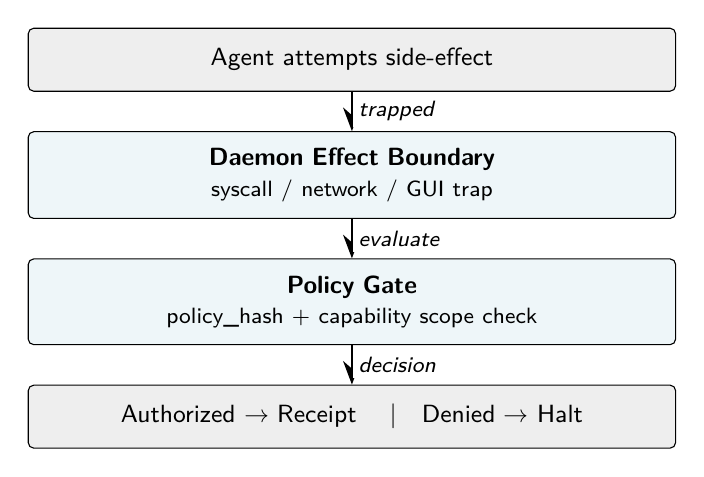
\begin{tikzpicture}[scale=1,transform shape,node distance=5mm and 10mm]
\node[ioiplain,text width=78mm] (req) {Agent attempts side-effect};
\node[ioibox,text width=78mm,below=of req] (fw) {\textbf{Daemon Effect Boundary}\\\footnotesize syscall / network / GUI trap};
\draw[ioiflow] (req) -- node[ioilabel,right]{trapped} (fw);
\node[ioibox,text width=78mm,below=of fw] (gate) {\textbf{Policy Gate}\\\footnotesize policy\_hash + capability scope check};
\draw[ioiflow] (fw) -- node[ioilabel,right]{evaluate} (gate);
\node[ioiplain,text width=78mm,below=of gate] (out) {Authorized $\rightarrow$ Receipt \quad|\quad Denied $\rightarrow$ Halt};
\draw[ioiflow] (gate) -- node[ioilabel,right]{decision} (out);
\end{tikzpicture}
\end{center}


The daemon effect boundary enforces a strict, four-step decision
pipeline at the validator ante level:

\begin{enumerate}
\def\labelenumi{\arabic{enumi}.}
\tightlist
\item
  \textbf{Intercept and Normalize:} When the agent attempts an
  externally-effectful operation, the hypervisor intercepts the request
  and normalizes it into a canonical \emph{ActionRequest}. This object
  contains a typed target (e.g., \emph{gui::click}), deterministic
  parameters, and the execution context.
\item
  \textbf{Translate Policy Context:} The engine loads the active,
  state-backed PolicyEnvelope and versioned rule set. Rule-set schemas are
  compatibility representations; the canonical boundary is the policy
  envelope bound to applicable authority, Agentgres state, and receipt
  obligations. The bundle includes applicable namespaced ontology-version and
  action-contract policies,
  per-target guardrails, and environment capability scopes (e.g.,
  restricted filesystem paths).
\item
  \textbf{Enforce (Context-Aware):} The request is deterministically
  evaluated against the ruleset at the exact moment of execution:
\end{enumerate}

\begin{itemize}
\item
  \begin{itemize}
  \tightlist
  \item
    If a matching cryptographic \emph{ApprovalToken} is presented for
    the exact request hash, the action is explicitly allowed.
  \item
    Otherwise, rule matching applies (\emph{Allow} / \emph{Block} /
    \emph{RequireApproval}).
  \item
    \textbf{PII Egress Routing:} If the action involves data egress, the
    daemon routes the payload through a local PII review contract. Here,
    the deterministic inspection/evaluator path
    identifies and masks sensitive data before it leaves the local
    boundary.
  \item
    All rejections are fail-closed.
  \end{itemize}
\end{itemize}

\begin{enumerate}
\def\labelenumi{\arabic{enumi}.}
\tightlist
\item
  \textbf{Emit Audit Trail:} The daemon emits transaction records and
  auditable outcomes as signed receipts and events (e.g.,
  \emph{EffectBoundaryInterception}, \emph{PiiDecisionReceiptEvent}),
  ensuring every execution decision is preserved for replayability and
  deterministic arbitration.
\end{enumerate}

Context-Aware Guardrails

Because the daemon effect boundary sits at the Hypervisor level, its
context awareness is real, not heuristic. Conditions are evaluated
against live session, OS, browser, workspace, and provider state through
mediated adapters. For example:

\begin{itemize}
\tightlist
\item
  \emph{allow\_apps} constraints validate the active window for
  \emph{gui::*} actions. This prevents \textbf{"Context Hijacking,"}
  where a malicious agent waits for the user to open a sensitive
  application (like a password manager) before triggering a seemingly
  benign allowed click.
\item
  Click coordinates are mathematically bounded to the active window
  geometry.
\item
  Network actions require strict URL-domain allowlists at the proxy
  level.
\item
  System command execution is constrained by safe command allowlists and
  command-class bans.
\end{itemize}

The Interception Boundary (\emph{RequireApproval})

The daemon effect boundary functions as the governance boundary between
the agent\textquotesingle s logic and the host\textquotesingle s
authority.
If a high-risk step triggers a \emph{RequireApproval} policy, the
daemon returns a \emph{PendingApproval} state and pauses the
agent\textquotesingle s execution. This triggers the UI to request
explicit human consent. Upon receiving a \emph{resume} command with a
valid cryptographic signature from the user, the daemon
deterministically verifies the token and allows the OS interaction to
proceed.

\hypertarget{actionrequest-the-canonical-action-primitive}{%
\subsubsection{2.6.1 ActionRequest: The Canonical Action
Primitive}\label{actionrequest-the-canonical-action-primitive}}

To be enforceable, policies must evaluate deterministic inputs. The
firewall therefore requires every outbound operation to be translated
into a normalized \emph{\textbf{ActionRequest}}. The
\emph{\textbf{ActionRequest}} is the pre-effect transaction candidate: a
canonical representation of the act before authority is granted or
execution occurs. This aligns with the Model Context Protocol while
adding the strict typing required for security.

The kernel normalizes inputs into the following schema before hashing:

\begin{itemize}
\item
  \textbf{Typed Target:} The namespaced identifier, covering both
  standard and native capabilities:

  \begin{itemize}
  \tightlist
  \item
    \emph{Standard MCP: fs::write}, \emph{net::fetch},
    \emph{wallet::send}, \emph{sys::exec}.
  \item
    \emph{Native Core (GUI):} \emph{gui::click}, \emph{gui::type}
    (OS-level Kinetic actions).
  \item
    \textbf{Headless Browser:} \emph{browser::navigate},
    \emph{browser::click\_selector}, \emph{browser::eval},
    \emph{browser::screenshot} (Hermetic DOM actions).
  \end{itemize}
\item
  \textbf{Arguments:} A canonical, schema-validated JSON payload (RFC
  8785) containing the tool parameters.
\item
  \textbf{Payload Storage:} Large input/output payloads (e.g., retrieval
  documents, datasets, packages, or model payloads) \textbf{MUST} be
  referenced through Agentgres-governed ArtifactRefs/PayloadRefs and,
  where useful, content-addressed commitments. A CID or hash proves bytes;
  it does not by itself authorize access, define artifact meaning, or make
  proprietary model weights safe to mount on an untrusted provider.
  Small payloads \textbf{MAY} be inlined when policy permits.
\item
  Context Bindings:

  \begin{itemize}
  \tightlist
  \item
    \emph{policy\_hash}: The hash of the active ruleset.
  \item
    \emph{session\_id}: The session identifier (if applicable).
  \item
    \emph{origin}: The ID of the agent requesting the action.
  \item
    \emph{window\_id} (Optional): For GUI actions, binding the click to
    a specific OS window handle to prevent clickjacking.
  \end{itemize}
\end{itemize}

\begin{longtable}[]{@{}>{\raggedright\arraybackslash}p{\linewidth}@{}}
\toprule\noalign{}
 \\
\midrule\noalign{}
\endhead
\bottomrule\noalign{}
\endlastfoot
\textbf{Normative Invariant:}\emph{\textbf{ }}This structure prevents
bypass via alternate toolpaths (e.g., trying to access the network via
\emph{browser::fetch} instead of \emph{net::fetch}). The Hypervisor Daemon
maps all drivers and MCP servers into the same target namespace,
creating a unified \textbf{daemon action surface} for agency where every action,
regardless of source, produces an identical, hashable receipt. \\
\end{longtable}

\hypertarget{actionrules-the-policy-language}{%
\subsubsection{2.6.2 Policy Envelopes and Versioned Rule
Sets}\label{actionrules-the-policy-language}}

Daemon effect policies are expressed as versioned policy bundles bound
to wallet.network authority, Agentgres state, capability scopes,
approval thresholds, budget limits, declassification rules, and receipt
obligations. A \emph{PolicyEnvelope} binds the selected versioned policy
schema and canonical rule content. Exact rule schemas belong to the policy
and wallet/daemon owners rather than this synthesis. Policies are default-deny
and may support graph-aware permissioning. The selected schema determines
matching, precedence, decision values, canonicalization, and evaluation
semantics; implementations may not infer those rules from unordered source
data. Security-critical deterministic inspection must not depend on
uncontrolled floating-point, locale, clock, random, or thread-scheduling
behavior. See Appendix A.1 for a non-exhaustive policy example rather than a
second policy-language specification.

\hypertarget{canonical-policy-ordering-hashing-normative}{%
\subsubsection{2.6.3 Versioned Policy Canonicalization and
Hashing}\label{canonical-policy-ordering-hashing-normative}}

A PolicyEnvelope binds a versioned policy schema, canonicalization function,
evaluation semantics, and policy hash. The owner contract must specify whether
rule order is meaningful, how maps, arrays, strings, numbers, identifiers, and
duplicates normalize, which canonical encoding is used, and whether evaluation
consumes the same representation that was hashed.

The invariant is representation fidelity: two implementations claiming the
same policy profile must produce the same canonical bytes and decision for the
same valid input, while malformed or unsupported versions fail closed. Raw
HashMap iteration, locale-dependent comparison, and source insertion order
must not silently change a policy hash or decision unless the owner schema
explicitly makes order semantic.

RFC 8785 JCS is the default JSON canonicalization reference where the selected
owner profile uses JSON. Exact sorting keys, precedence rules, Unicode handling,
and hash algorithms remain in that profile; the example in Appendix A.1 is
illustrative and does not establish a second normative policy language.
\hypertarget{deterministic-inspection-assist-profile-policy-enforcement-over-a-local-evidence-graph}{%
\subsubsection{2.6.4 Deterministic Inspection Assist Profile: Policy Enforcement
over a Local Evidence
Graph}\label{deterministic-inspection-assist-profile-policy-enforcement-over-a-local-evidence-graph}}

A decentralized agent system cannot treat arbitrary neural inference as
a consensus primitive. Open-ended model execution varies across
hardware, runtimes, compiler settings, and vendor-specific kernels. Even
when two environments produce semantically similar outputs, they are not
a safe basis for policy gates, receipts, or replay-critical validation.
IOI addresses this by separating cognitive inference from enforcement:
models may propose, but the enforcement path must reduce those proposals
to deterministic, replayable structures before they can cross a trust
boundary.

Consensus on Enforcement, Not General Cognition

The goal of the deterministic inspection assist profile is not to
reproduce a full model\textquotesingle s internal reasoning across
nodes. The goal is narrower and more useful: consensus on
policy-relevant classification and action gating. For
PII-sensitive egress, IOI first builds a local evidence graph using
deterministic detectors and validators for concrete classes such as API
keys, emails, phone numbers, SSNs, and card PANs. The assist profile
then operates on that evidence graph, not on raw probabilistic hidden
states. If two
nodes begin from the same evidence graph, policy, target, and risk
surface, they derive the same assist identity, routing outcome, and
decision hash.

A Candidate Assist Profile: Narrow and Deterministic

A candidate profile such as \emph{inspection\_v0} could be a narrow
deterministic assist contract, not a generalized quantized LLM. Its role is to refine
ambiguous spans in a strictly bounded way before routing and transform
decisions are made. Its allowed behaviors are intentionally limited: it
may drop spans that are deterministically identified as ambiguity false
positives, downgrade confidence buckets, and clear ambiguity in specific
policy-defined cases. It may not create new spans, mutate the source
hash, increase severity, or upgrade a classification to a more severe
class. This keeps the safety layer legible, auditable, and
consensus-friendly.

Deterministic Runtime Properties

The assist contract forbids wall-clock reads, RNG, external I/O,
locale-sensitive behavior, and floating-point or thread-scheduling
dependence. The surrounding PII pipeline is likewise structured around
deterministic evidence extraction, rules-only routing, and deterministic
transform. In practice, this means the safety decision is driven by
stable local detectors, explicit policy controls, and an assist receipt
that is bound into decision-hash material. A locally produced PII
decision can therefore be validated and replayed without depending on
arbitrary model execution.

\begin{longtable}[]{@{}>{\raggedright\arraybackslash}p{\linewidth}@{}}
\toprule\noalign{}
 \\
\midrule\noalign{}
\endhead
\bottomrule\noalign{}
\endlastfoot
\textbf{Status Note: }This synthesis does not claim a deployed
\emph{inspection\_v0} profile. Any implementation must be established by its
canonical owner and conformance tests and must carry explicit assist identity,
version, configuration, module, evidence, and receipt bindings. It must not be
marketed as a generalized integer-only model or protocol-wide WASM safety guest. \\
\end{longtable}

\begin{longtable}[]{@{}
  >{\raggedright\arraybackslash}p{(\columnwidth - 0\tabcolsep) * \real{1.0000}}@{}}
\toprule\noalign{}
 \\
\midrule\noalign{}
\endhead
\bottomrule\noalign{}
\endlastfoot
\textbf{Normative Invariant}\emph{\textbf{:}}

The validity of the daemon effect boundary must not depend on
reproducing open-ended cognitive inference on verifier hardware.
Safety-critical policy decisions must be reducible to deterministic evidence,
explicit policy state, the applicable authority refs, and a versioned,
verifiable assist contract. \\
\end{longtable}

\hypertarget{the-capability-surface-primitive-constraints-vs.-authority-scopes}{%
\subsubsection{2.6.5 The Capability Surface: Primitive Constraints vs.
Authority
Scopes}\label{the-capability-surface-primitive-constraints-vs.-authority-scopes}}

The Bifurcated Capability Surface

To prevent security bypasses and ambiguous authority boundaries, IOI abandons
flattened capability bags. The capability surface is strictly bifurcated
into two tiers:

\begin{itemize}
\tightlist
\item
  \textbf{Primitive Execution Capabilities
  (}\emph{\textbf{prim:*}}\textbf{):} These describe runtime
  feasibility, physical isolation, and risk boundaries enforced by the
  Hypervisor Daemon. Examples: \emph{prim:fs.read},
  \emph{prim:fs.write}, \emph{prim:sys.exec}, \emph{prim:ui.interact},
  \emph{prim:net.request}, \emph{prim:model.invoke}.
\item
  \textbf{Authority Scopes (}\emph{\textbf{scope:*}}\textbf{):} These
  describe authority-provider admission policies, budgets, and identity
  constraints. wallet.network governs portable delegated, secret-bearing,
  spend-bearing, declassification, cross-domain, and high-risk external
  scopes; local/domain owners may govern ordinary local scopes. Examples:
  \emph{scope:gmail.read}, \emph{scope:gmail.send},
  \emph{scope:commerce.order\_submit}, \emph{scope:repo.write}.
\end{itemize}

Every tool and connection MUST define a \emph{RuntimeToolContract} that
declares both its required \emph{prim:*} capabilities and its
\emph{scope:*} authority boundaries. The Hypervisor Daemon enforces
primitive feasibility; the applicable authority provider enforces authority
admission. Together, they prevent the "confused deputy" failures that
arise when execution capability and resource authority are conflated
into a single permission bag.

\hypertarget{capability-scopes-permissions-not-root}{%
\subsubsection{2.6.6 Capability scopes: permissions, not
root}\label{capability-scopes-permissions-not-root}}

Agents are granted \textbf{scoped capabilities} rather than ambient
authority, ensuring they operate within a "Safety Envelope":

\emph{prim:net.request} bounded by \emph{scope:domain\_allowlist} ---
outbound allowlists (domains/IP ranges), protocol restrictions, and
per-origin limits.

\emph{prim:fs.read} / \emph{prim:fs.write} --- read/write scopes
restricted to sandboxed roots; explicit deny lists for secrets
(\emph{\textasciitilde/.ssh}, \emph{/etc}, keychains).

\emph{prim:ui.interact} bounded by \emph{scope:ui.application} --- UI
control limited to specific window/application identifiers and interaction
types.

\emph{scope:wallet.transfer\_under\_limit} --- hard ceilings for work
credits, settlement assets, and any wallet/transaction operations
(per-session and per-day).

\emph{prim:sys.exec} bounded by an executable policy --- restrictions on
creating child processes or accessing system binaries (e.g., "Allow
\emph{ffmpeg}, Block \emph{bash}").

Capabilities define the maximum possible envelope; the daemon policy
bundle defines the per-action policy inside that envelope. Concrete rule
representations remain versioned owner contracts.

\hypertarget{interception-and-approvals}{%
\subsubsection{2.6.7 Interception and
approvals}\label{interception-and-approvals}}

1. \textbf{Request:} The active runtime substrate emits an
ActionRequest (e.g., \emph{gui::click\{x,y,window\_id\}}). The
substrate may be a process sandbox, container, VM, microVM, WASM worker,
browser sandbox, GPU job, TEE enclave, or other daemon-approved
execution lane.

2. \textbf{Evaluation:} The Hypervisor Daemon evaluates primitive
feasibility and policy, then requests the applicable authority provider.
wallet.network is mandatory where a portable delegated grant, secret lease,
spend, declassification, cross-domain reuse, or high-risk external effect is
required.

3. \textbf{Settlement Resolution:}

* \textbf{ALLOW: }forward to the relevant driver.

* \textbf{BLOCK:} drop the request and return \emph{AccessDenied}.

* \textbf{REQUIRE\_APPROVAL:} pause execution and prompt the user via
the IOI UI.

Approval tokens (formalizing ``user consent''):

User approvals are issued as \textbf{signed approval tokens} with
explicit scope (target + constraints), TTL, and optional usage count
(one-time vs session). Tokens are recorded in the audit chain and can be
replay-checked to prevent silent reuse. This acts as \textbf{2FA for
Agency}, ensuring critical actions (like spending) require explicit
human sign-off. Approval therefore carries Own into Act. The user is not
merely clicking OK; they are signing bounded execution authority for a
specific transaction-shaped action.

\hfill\break
When an action triggers \emph{REQUIRE\_APPROVAL}, the
applicable authority provider authorizes a scoped approval artifact. For a
wallet.network step-up, issuance follows evaluation of the
\emph{AccessPointBinding} and resolution of the \emph{StepUpChallenge}. To
prevent replay and bypass attacks, the artifact MUST bind:

\begin{itemize}
\tightlist
\item
  \emph{request\_hash} (the canonical intent)
\item
  \emph{policy\_hash} (the active policy state)
\item
  \emph{visual\_hash} (SHOULD be bound for GUI/screen-based actions)
\item
  \emph{audience} (Validator/Executor identity)
\item
  \emph{expiry} (time bound; Chain Time / Block Height)
\item
  \emph{revocation\_epoch} (minimum valid epoch for bulk revocation)
\item
  \emph{counter} (Monotonic nonce)
\end{itemize}

Tokens may be \textbf{One-Shot} (burned upon execution) or
\textbf{Multi-Use} (Lease). Multi-use tokens MUST strictly decrement a
\emph{max\_usages} counter recorded in the state receipt log.

Gate Results and Decision Receipts

The runtime MUST produce a \emph{GateResult} and receipt ref for every
consequential governed action. It records the ActionProposal, policy hash,
applicable authority refs, result, reason, blocker or safe alternatives, and
decision receipt. The binding makes the declared decision replayable; it does
not by itself prove faithful policy enforcement outside the admitted boundary.

\hypertarget{audit-and-portability}{%
\subsubsection{2.6.8 Audit and
portability}\label{audit-and-portability}}

Every daemon effect decision is appended to the local receipt chain, creating
\textbf{the Economic Chain of Custody by which executable ownership
remains replayable and settleable}:

\begin{itemize}
\tightlist
\item
  \emph{action\_hash} (canonicalized request)
\item
  policy\_hash
\item
  \emph{resolution} (+ approval token reference if applicable)
\item
  \emph{timestamp/sequence} (daemon or wallet.network authority-profile linked)
\end{itemize}

Policies themselves are content-addressed (hashed), enabling:

\begin{itemize}
\tightlist
\item
  \textbf{Sharing:} developers publish hardened policies (e.g., ``Safe
  Banking'', ``Read-Only Email'').
\item
  \textbf{Auditing:} third parties verify an agent operated under a
  declared policy set.
\item
  \textbf{Enforcement:} when outcomes escalate to network settlement,
  the daemon or wallet.network authority path attests
  to the \emph{policy\_hash}. Artifacts whose bindings do not match the
  declared policy are invalid for higher tiers.
\end{itemize}

This turns the user device from a passive terminal into a
\textbf{managed runtime}: autonomy is real, but it is bounded by
explicit, verifiable constraints that limit \textbf{Liability}.

\hypertarget{normative-schema-firewall-artifacts}{%
\subsubsection{2.6.9 Effect Boundary Object
Family}\label{normative-schema-firewall-artifacts}}

The Hypervisor Daemon effect boundary uses current HarnessProfile objects to
ensure interoperability: \textbf{ActionProposal} (the normalized proposed
act and its primitive/scope needs), \textbf{GateResult} (the policy and
authority result with a receipt ref), and \textbf{NormalizedObservation}
(typed reality returned to the loop). Wallet approvals or grants remain
separate authority artifacts referenced by the gate result.
All hashes are computed over RFC 8785 canonicalized bytes;
\emph{policy\_hash} MUST be stable for a given ordered ruleset. Full
Illustrative field summaries are in Appendix A.2; canonical owner documents
govern exact schemas and canonicalization requirements.

\hypertarget{attribution-graphs-contribution-receipts}{%
\subsubsection{\texorpdfstring{2.6.10 \textbf{Attribution} Graphs \&
Contribution
Receipts}{2.6.10 Attribution Graphs \& Contribution Receipts}}\label{attribution-graphs-contribution-receipts}}

To scale agency beyond simple tasks, IOI supports Marketplace Neutrality
and Contribution Accounting. These primitives ensure that delegated work
graphs remain economically legible and that upstream contributors retain
credit even when their work is composed into downstream outcomes.

Anti-Cannibalization Rule

The \textbf{Hypervisor Daemon} is the execution substrate, and it
mediates HarnessProfiles under loop-native conformance; the
\textbf{Default Harness Profile} is the reference scaffold/fallback and
possesses no substrate mechanics separate from the daemon. As that
substrate, the daemon MUST remain neutral: it is forbidden by
conformance, policy, and marketplace-neutrality doctrine from silently
cloning, absorbing, or reproducing third-party worker logic into native
primitives. Marketplace neutrality is enforced at the protocol level:
the runtime cannot use its privileged position to displace the very
contributors whose work it routes.

Contribution Receipts

When an agent hires another worker or uses a specialized tool, Agentgres
records a \emph{ContributionReceipt}. This receipt tracks the
\emph{quality\_delta} the contribution introduced and binds the
contributor's identity into the downstream outcome's provenance chain.
When the downstream task settles successfully, \emph{wallet.network}
uses the contribution graph to route compensation or credit attribution
to upstream providers in proportion to their measured contribution.

The Contribution Graph (Agentgres)

Agentgres maintains the canonical Contribution Graph for each domain: a
directed acyclic record of who hired whom, under what authority budget,
with what measured quality contribution. This replaces the prior
``Delegation Graph Ledger'' abstraction with a marketplace-neutral
object whose semantics are economic accounting first, runtime sub-hiring
second. The graph is queryable as a first-class projection and is
admissible as evidence in dispute resolution.

\hypertarget{proposal-mediated-upgrades-upgrade-governance}{%
\subsubsection{2.6.11 Proposal-Mediated Upgrades \& Upgrade
Governance}\label{proposal-mediated-upgrades-upgrade-governance}}

To enable safe autonomous improvement, improvement is re-framed as a
governed, proposal-mediated upgrade process. Agents do not self-modify
directly. Instead, autonomous systems propose upgrades to governed
modules, workflows, skills, memory projections, routes, and policies,
and only policy-bound, receipted governance makes those upgrades
canonical.

When an autonomous system identifies a performance limitation, it
executes the following upgrade pipeline:

1. Observe limitation \& draft an Upgrade Proposal.

2. Bind the target module, workflow, policy, tool, model route, or
schema.

3. Simulate, evaluate, benchmark, or dry-run the proposed changes.

4. Review the upgrade under current policy and authority.

5. Approve, reject, escalate, or roll back.

6. Commit the accepted operation through the daemon into Agentgres.

7. Emit Upgrade Receipts and optional IOI L1 anchored roots.

The receipt set is typed. A \textbf{ContextMutationReceipt} binds a
versioned context update, contradiction, supersession, or deprecation to
evidence, policy, authority, and worker/project refs. A
\textbf{PromotionDecisionReceipt} binds a context, adapter, route-policy,
evaluation, package, skill, or workflow promotion decision to
baseline/candidate versions, regression checks, gates, rollback refs,
and policy. Training, benchmark, evaluation, and routing effects use the
same receipt family as Worker Training:
\textbf{TrainingReceipt}, \textbf{BenchmarkReceipt},
\textbf{EvaluationReceipt}, and \textbf{RoutingDecisionReceipt}.

This process strictly enforces the \textbf{Monotonic Policy Invariant}
(\emph{Policy\_New} must be a strict subset or equivalent of
\emph{Policy\_Old}) at the boundary, ensuring logic can be optimized but
privileges cannot be expanded without explicit step-up signature
authorization.

\begin{longtable}[]{@{}
  >{\raggedright\arraybackslash}p{(\columnwidth - 0\tabcolsep) * \real{1.0000}}@{}}
\toprule\noalign{}
 \\
\midrule\noalign{}
\endhead
\bottomrule\noalign{}
\endlastfoot
The Subset Inclusion Invariant:

An upgrade is valid \textbf{IF AND ONLY IF} \emph{Policy\_New} is a
strict subset or equivalent of \emph{Policy\_Old
$\subseteq$}.

\begin{itemize}
\tightlist
\item
  \textbf{Allowed:} "I want to \emph{remove} my access to the filesystem
  because I don\textquotesingle t need it." (Tightening constraints).
\item
  \textbf{Allowed:} "I want to change my system prompt to be more
  polite." (Logic change, Constraint unchanged).
\item
  \textbf{BLOCKED:} "I want to \emph{add} access to api.stripe.com."
  (Loosening constraints).
\item
  \textbf{BLOCKED:} "I want to increase my daily spend limit."
  (Loosening constraints).
\end{itemize} \\
\end{longtable}

This prevents an accepted upgrade from silently widening its own declared
authority. It does not prove that changed logic is harmless. Any proposed
constraint relaxation requires a new, explicit authority and policy decision
under the applicable owner contract.

Continuity Proofs

A future \textbf{High-Assurance Continuity Profile} (Section 9.4.4) may
require a versioned continuity record carrying an accumulator and proof for a
precisely specified transition predicate. Under such a profile, an upgrade
lacking the required proof is rejected and the existing manifest remains
canonical. No particular record name, proof backend, or recursive circuit is
canonized by the current architecture owners.

\hypertarget{state-memory-and-semantic-data}{%
\section{3. State, Memory, and Semantic
Data}\label{state-memory-and-semantic-data}}

Traditional web applications rely on a centralized relational database
as the source of truth, with blob storage for files and caches for
speed. Decentralized agentic applications require a different
foundation: canonical replayable operations, portable serving across
untrusted nodes, and cryptographic receipts. A centralized database
cannot serve as the ultimate source of truth for decentralized, portable
agency.

To replace this legacy stack, IOI uses a kernel-native state and memory
architecture with two complementary planes. \textbf{Agentgres} is
admitted operational truth: the canonical operation log and its
materialized projections, serving the role traditionally held by a
centralized database without inheriting mutable-row truth semantics.
\textbf{Agent Wiki / \emph{ioi-memory}} is the semantic context-memory
plane: the agent's local execution history, document corpus, learned
tool affordances, workspace facts, and vector embeddings, serving the
  role traditionally held by a user's personal context. Authoritative
  execution history, however, is not held in this fuzzy substrate: it
  consists of admitted operations and receipts carrying their declared
  assurance stage inside Agentgres, which Agent Wiki / ioi-memory indexes for
  semantic retrieval. Receipt presence alone does not imply verification,
  acceptance, adjudication, or settlement.

IOI separates state, memory, and semantic data:

\begin{enumerate}
\def\labelenumi{\arabic{enumi}.}
\tightlist
\item
  \textbf{Agentgres} stores canonical operational truth: accepted
  operations, object heads, state roots, projections, subscriptions,
  receipts, ledgers, and archive refs.
\item
  \emph{ioi-memory} stores private semantic memory, retrieval surfaces,
  references to execution traces, and task-scoped context.
\item
  \textbf{Domain Ontologies and Data Recipes} define domain meaning and
  transform raw sources into ontology-bound runtime, training,
  evaluation, and projection data.
\end{enumerate}

\begin{enumerate}
\def\labelenumi{\arabic{enumi}.}
\tightlist
\item
  \textbf{Agentgres:} The \emph{Application's Truth}. Agentgres rejects
  the premise that mutable database rows are the source of truth.
  Canonical truth is the deterministic operation log; app-facing reads
  are materialized as strictly verifiable \emph{Agentgres Projections}.
\item
  \textbf{Agent Wiki / \emph{ioi-memory}:} The \emph{Worker's Memory}
  and semantic context plane. It governs what the worker knows,
  providing tiered memory (working, core, archival), vector search,
  learned tool affordances, route preferences, wiki facts, and privacy
  slicing. Archival and core memory mutations are not direct file
  operations; they must be written to the Agentgres Artifact Plane via
  \emph{ContextMutation} commits before they count as durable or
  portable state.
\end{enumerate}

\hypertarget{agentgres-operation-backed-domain-truth}{%
\subsection{3.1 Agentgres: Operation-Backed Domain
Truth}\label{agentgres-operation-backed-domain-truth}}

Agentgres is the operational truth substrate for governed
autonomous-system chains and Hypervisor Node local settlement domains.
It records proposals, module invocations, local settlement records,
receipt roots, upgrade decisions, state roots, and replayable
projections.

For collective pursuit, Agentgres records the admitted per-domain
\textbf{OutcomeRoom} and \textbf{CollaborativeWorkGraph} state: discovery and
participation decisions, participant leases and portable exit bundles,
resource and capability offers, frontier items, claim leases, attempts,
findings, verifier challenges, generic WorkResults, OutcomeDeltas,
contribution lineage, and replay refs. It records what a domain admitted; it
does not make a room, message board, or federation into one globally mutable
truth database.

Each serious Web4 application domain (e.g., \emph{aiagent.xyz},
\emph{sas.xyz}, enterprise deployments) runs its own kernel/runtime
deployment with its own independent Agentgres domain.

Agentgres stores:

\begin{enumerate}
\def\labelenumi{\arabic{enumi}.}
\tightlist
\item
  governed autonomous-system chain records;
\item
  Hypervisor-node local settlement records;
\item
  service module manifests and registry roots;
\item
  module invocation records;
\item
  proposal queues and upgrade decisions;
\item
  admitted operations and domain sequence numbers;
\item
  object heads and state roots;
\item
  schema versions;
\item
  constraints and invariants;
\item
  policy hashes;
\item
  authority grant refs;
\item
  artifact refs;
\item
  projection definitions and checkpoints;
\item
  subscription watermarks;
\item
  receipt metadata;
\item
  OutcomeRoom discovery, participation, lease, exit, frontier, claim,
  attempt, finding, challenge, WorkResult, OutcomeDelta, and replay objects;
\item
  ontology versions, overlays, assertions, crosswalks, semantic mapping
  decisions, and ontology action contracts;
\item
  quality/contribution ledgers;
\item
  settlement mirrors;
\item
  archive refs and restore receipts.
\end{enumerate}

Agentgres state is \textbf{domain-local operational truth}. A domain may
publish state roots, registry roots, settlement mirrors, receipt roots,
or dispute commitments to IOI L1, but ordinary projection state, traces,
subscriptions, runtime state, and worker-training state stay in the
domain kernel unless a public commitment is required.

An OutcomeRoom therefore names its shared-state admission owner. In
\texttt{hosted\_admission}, the host domain sequences and admits the room
projection. In \texttt{federated\_admission}, a versioned policy declares the
member domains, ordering or merge rules, conflicts, quorum or adjudicator,
failover, and recovery. Each participant still admits its own private work and
outbound claims locally. AIIP carries signed refs and permitted deltas between
those boundaries; packet arrival, participant consensus, or leaderboard state
is evidence input rather than automatic Agentgres admission.

Each serious domain should have its own Agentgres kernel:

\begin{enumerate}
\def\labelenumi{\arabic{enumi}.}
\tightlist
\item
  agentgres://domain/local-hypervisor-user
\item
  agentgres://domain/ioi.ai
\item
  agentgres://domain/aiagent.xyz
\item
  agentgres://domain/sas.xyz
\item
  agentgres://domain/enterprise-customer
\item
  agentgres://domain/sovereign-worker-network
\end{enumerate}

These domains may reference one another explicitly, but they should not
share one giant mutable Agentgres state. \textbf{Cross-domain
references} bind object refs, state roots, manifest hashes, policy
hashes, receipt roots, room-admission watermarks, semantic mapping decisions,
restricted views, and settlement mirrors. A hosted room database is never a
portability dependency: a departing participant may retain a signed,
policy-filtered ParticipantStateBundle whose historical proof remains usable
without continued access to the room host.

Agentgres operates across a rigorous, decoupled data stack:

\begin{enumerate}
\def\labelenumi{\arabic{enumi}.}
\tightlist
\item
  \textbf{The Canonical Operation Log (The Deepest Truth):} The state
  machine does not mutate rows in place. Every state change is a signed,
  canonical operation appended to the log. Truth is historical and
  replayable.
\item
  \textbf{The Object Model:} A semantic object framework built over the
  canonical state log. It holds domain entities like \emph{Service},
  \emph{Version}, \emph{Run}, \emph{Receipt}, \emph{CapabilityLease},
  \emph{OutcomeRoom}, \emph{WorkFrontierItem}, \emph{Attempt},
  \emph{Finding}, \emph{WorkResult}, \emph{OutcomeDelta}, and the federated
  ontology object families (object-first truth, not row-first truth).
\item
  \textbf{The Projection Engine:} The computational engine that
  maintains materialized read models, derived indexes, real-time
  changefeeds, and projection checkpoints.
\end{enumerate}

\textbf{The Replay Invariant:} Because all truth originates from the
canonical operation log, any node can independently reconstruct the
current state of the application by replaying the signed operations from
genesis to the current \emph{agentgres\_projection\_watermark}.

\hypertarget{the-agentgres-artifact-plane-and-storage-boundaries}{%
\subsection{3.2 The Agentgres Artifact Plane and Storage
Boundaries}\label{the-agentgres-artifact-plane-and-storage-boundaries}}

To prevent state corruption and to avoid the critical security flaw of
trusting storage layers with protocol authority, the Hypervisor enforces
a strict boundary between the \textbf{Agentgres Artifact Plane} and
passive \textbf{Storage Backends}.

Storage backends (such as Filecoin, IPFS, S3, or local disk partitions)
are strictly passive byte repositories. They do not possess authority,
they do not understand schemas, and they cannot validate the
cryptographic lineage of the data they hold. Raw bytes retrieved from a
storage backend do not constitute canonical evidence, a valid delivery,
or portable state unless they are bound to an \emph{ArtifactRef} or
\emph{PayloadRef} registered within the \textbf{Agentgres Artifact
Plane}.

The \textbf{Agentgres Artifact Plane} is the canonical meaning,
admission, and lifecycle layer for operational artifact semantics,
state-root validity, and structural lifecycle management. It is not an
authority provider. When a worker generates an output (e.g., a PDF, a
dataset, or a state archive), the Hypervisor Daemon commits the
metadata, policy linkages, and cryptographic receipts to Agentgres,
mapping these to the raw bytes via content-addressed identifiers.

Backend availability is also represented as admitted operational state.
If a payload ref is missing, stale, unavailable, fails hash validation,
or cannot be retrieved from its declared backend, the daemon records an
\textbf{ArtifactAvailabilityIncident} in Agentgres. Repair, replica
selection, backend migration, archive regeneration, or replacement
binding must emit an \textbf{ArtifactRepairReceipt}. These records do
not make Filecoin, IPFS, S3, local disk, or any object store the truth
layer; they make storage failure and recovery accountable under the
Agentgres artifact lifecycle.

For artifacts that can become dispute evidence, availability incidents
are not merely telemetry. During a live challenge epoch, failure to serve
the bytes named by an admitted ArtifactRef or PayloadRef before the
declared retrieval deadline creates a valid \emph{MissingEvidence}
challenge. Agentgres remains the semantic truth layer, but the protocol
requires enough data availability to reconstruct the challenged trace.
Storage backends may hold the bytes; Agentgres records the commitments,
retention bounds, repair receipts, and challenge consequences.

\textbf{Storage, meaning, and authority boundary.}

\begin{longtable}[]{@{}
  >{\raggedright\arraybackslash}p{(\linewidth - 4\tabcolsep) * \real{0.3333}}
  >{\raggedright\arraybackslash}p{(\linewidth - 4\tabcolsep) * \real{0.3333}}
  >{\raggedright\arraybackslash}p{(\linewidth - 4\tabcolsep) * \real{0.3333}}@{}}
\toprule\noalign{}
& & \\
\midrule\noalign{}
\endhead
\bottomrule\noalign{}
\endlastfoot
Dimension / Asset & Agentgres Artifact Plane (Meaning / Lifecycle) & Storage
Backends (Passive Byte Storage) \\
\textbf{Data Owned} & \emph{ArtifactRef}, \emph{PayloadRef},
\emph{EvidenceBundle}, \emph{DeliveryBundle}, and
\emph{AgentStateArchive}. & Raw blocks, blobs, and encrypted byte
arrays. \\
\textbf{Responsibilities} & Records policy and authority linkages;
validates structural lineage, state roots, receipt-to-action bindings,
artifact lifecycle, and restore validity. Applicable authority providers
authorize access and mutation. & Storing, retrieving, and serving requested
bytes by hash, key, or path. \\
\textbf{Trust Profile} & \textbf{Admitted Operational Truth.} Writes
cross daemon/domain admission under applicable local governance and
wallet.network authority. & \textbf{No Semantic or Execution Authority.}
Treated as an untrusted or volatile transport and storage channel. \\
\textbf{Valid Systems} & Local Agentgres instances, Domain Kernels, and
Mirror Nodes. & Local disk, AWS S3, Google Cloud Storage, Filecoin,
CAS/IPFS, and DePIN blob stores. \\
\end{longtable}

To prevent blockchain bloat and ensure fast execution, the architecture
enforces a strict separation between operational metadata and heavy
payloads.

Agentgres is not a thin index over Filecoin/CAS blobs.

\begin{enumerate}
\def\labelenumi{\arabic{enumi}.}
\tightlist
\item
  \textbf{Agentgres (Hot / Operational):} Owns the canonical operation
  log, object heads, constraints, indexes, projections, subscriptions,
  receipt metadata, delivery state, and quality/contribution ledgers.
\item
  \textbf{Storage Backends (Cold / Payload):} Store payload bytes behind
  Agentgres-governed refs: worker packages, large evidence objects, trace
  bundles, generated artifacts (PDFs/videos), and archival checkpoints.
  Filecoin, CAS/IPFS, S3, object stores, CDNs, and local disk are backend
  examples, not authority layers.
\end{enumerate}

\textbf{The Mechanism:} storage backends store payload bytes; Agentgres
stores the \emph{ArtifactRef}. The \emph{ArtifactRef} binds the
payload's Content Identifier (CID/Hash) to its provenance (which run
produced it, which receipt validates it, and what policy governs its
access).

\textbf{Managed worker instance lifecycle.} Managed worker instances may
keep small canonical refs \textbf{hot} and move heavy or idle state
\textbf{cold}. Hot state includes instance id, worker manifest ref,
lifecycle status, latest state root, runtime assignment, authority
policy, subscription/entitlement, archive CID/hash, policy hash, and
restore permissions. Cold state may include traces, context windows,
intermediate artifacts, inactive patch branches, cached projections,
checkpoints, and evidence bundles sealed as encrypted content-addressed
archives.

Agentgres has two planes.

\textbf{Hot canonical runtime state:} operation log; object heads;
task/run/patch state; projection checkpoints; active subscriptions;
leases; receipts; archive refs and lifecycle metadata.

\textbf{Cold durable artifact plane:} encrypted snapshots; trace
bundles; evidence bundles; replay exports; dormant agent/worker state;
large payloads; backups; sealed archives, including
\textbf{SealedStateArchive} payloads for inactive, idle, portable,
migrated, or restorable runtime/domain state.

Filecoin/CAS/S3/local disk may hold encrypted archive bytes by hash/CID.
\textbf{These bytes are not canonical live state.} Agentgres is the
authority that records the archive ref, state root, schema version,
policy hash, object heads, authority context, restore policy, and
receipts.

\textbf{Operation-backed restore and import.} State restoration is never
a silent, out-of-process local file mutation. The Hypervisor Daemon
executes state imports as canonical, operation-backed Agentgres
transactions.


\begin{center}
\needspace{6\baselineskip}
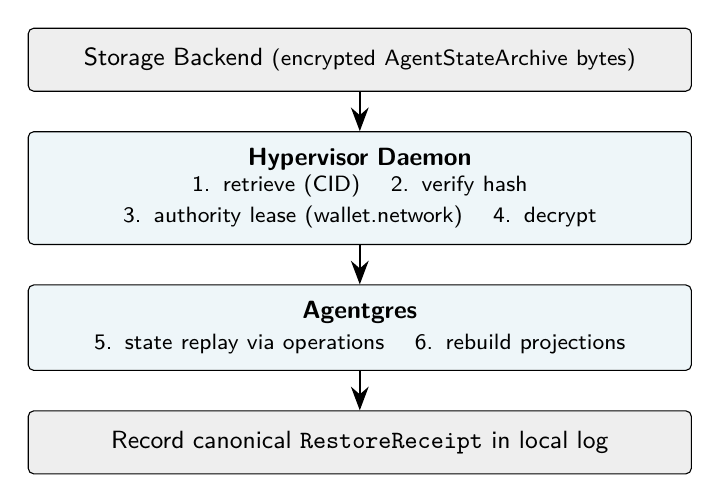
\begin{tikzpicture}[scale=1,transform shape,node distance=5mm and 10mm]
\node[ioiplain,text width=80mm] (sb){Storage Backend \footnotesize(encrypted AgentStateArchive bytes)};
\node[ioibox,below=of sb,text width=80mm] (hd){\textbf{Hypervisor Daemon}\\\footnotesize 1. retrieve (CID) \quad 2. verify hash\\ 3. authority lease (wallet.network) \quad 4. decrypt};
\node[ioibox,below=of hd,text width=80mm] (ag){\textbf{Agentgres}\\\footnotesize 5. state replay via operations \quad 6. rebuild projections};
\node[ioiplain,below=of ag,text width=80mm] (rr){Record canonical \texttt{RestoreReceipt} in local log};
\draw[ioiflow](sb)--(hd);\draw[ioiflow](hd)--(ag);\draw[ioiflow](ag)--(rr);
\end{tikzpicture}
\end{center}

in local log)

1. \textbf{Archive Retrieval:} the Hypervisor Daemon fetches the
encrypted \emph{AgentStateArchive} bytes from the designated Storage
Backend.

2. \textbf{Cryptographic Verification:} the retrieved bytes are hashed
and matched against the expected content-addressed identifier (CID) to
guarantee payload integrity.

3. \textbf{Authority Validation:} the daemon queries
\emph{wallet.network} to verify the requester's identity and obtain a
valid cryptographic key or short-lived decryption lease.

4. \textbf{Decryption:} the bytes are decrypted within the secure
hypervisor runtime.

5. \textbf{Agentgres Operation Import:} the state transitions are
ingested and parsed as a sequence of signed operations in the Agentgres
log, ensuring historical consistency and preventing arbitrary state
injection.

6. \textbf{Projection Reconstruction:} the projection engine rebuilds
the materialized database views, bringing the active workspace up to the
current state-root watermark.

7. \textbf{Receipt Recording:} the daemon generates and commits a
canonical \emph{RestoreReceipt} to the Agentgres log, permanently
recording who restored the archive, under which policy, and with what
valid receipt references.

\textbf{Secret handling.} Secrets should be represented by
wallet.network references or sealed key leases, not embedded as raw
secret material in state archives. Restore reacquires scoped authority
instead of replaying stale secret material.

\hypertarget{projections-subscriptions-the-agentgres-read-interface}{%
\subsection{3.3 Projections \& Subscriptions: The Agentgres Read
Interface}\label{projections-subscriptions-the-agentgres-read-interface}}

In traditional databases, indexes and views are hidden implementation
details. In IOI, \textbf{Projections are first-class, versioned protocol
artifacts.} Agentgres serves these projections directly to applications.

Agentgres supports multiple projection families natively:

\begin{enumerate}
\def\labelenumi{\arabic{enumi}.}
\tightlist
\item
  \textbf{Relational Projections:} For dashboards, billing summaries,
  and tabular admin views.
\item
  \textbf{Graph Projections:} For service dependency graphs, capability
  workflows, and lineage tracking.
\item
  \textbf{Timeline / Event Projections:} For run timelines, audit
  trails, and operation feeds.
\item
  \textbf{Capability Projections:} For resolving ``what this session can
  access'' or ``what this lease permits.''
\end{enumerate}

\textbf{Projection Watermarks:} Clients bind directly to these named,
versioned projections. Because projections are asynchronous, every read
from Agentgres includes an \emph{agentgres\_projection\_watermark}
(e.g., \emph{domain\_seq:99182}). This guarantees that the client knows
exactly which sequence of operations is reflected in the view.

\textbf{Postgres bridge.} Projections are first-class serving surfaces.
Agentgres may expose SQL or Postgres-compatible reads over named
projections for BI tools, admin tooling, dashboards, ORMs, and
psql-compatible clients. Projection reads must expose freshness, domain
sequence, policy, and source watermarks when relevant.

Projection compatibility does not imply mutable-row canonicality. Writes
become canonical only when compiled into Agentgres operations and
accepted under schema, authority, policy, constraints, invariants, and
receipt obligations.

The canonical bridge/readiness object names are explicit.
\textbf{AgentgresPostgresBridge} is a Postgres-compatible read/query
surface over named projections, not a mutable-row truth store.
\textbf{AgentgresConsistencyLevel} declares whether a read is
\emph{cached\_projection}, \emph{projection\_consistent},
\emph{snapshot\_consistent}, \emph{state\_root\_consistent},
\emph{linearized\_domain}, or \emph{serializable\_domain}.
\textbf{DomainSequence} is the ordered accepted-operation sequence for
an Agentgres domain; recovery restores to sequence N, verifies roots
through N, and rebuilds projections from verified checkpoints.
\textbf{AgentgresInvariant} covers validity rules such as authority,
receipt, settlement, policy, temporal, projection, state-root,
artifact-integrity, and policy-monotonicity requirements.
\textbf{AgentgresConstraint} covers object rules such as required
fields, schema types, unique keys, foreign refs, checks, exclusion
rules, cardinality, and temporal ranges.

\hypertarget{distributed-runtime-serving-managed-instances-and-subscriptions}{%
\subsection{3.4 Distributed Runtime Serving, Managed Instances, and
Subscriptions}\label{distributed-runtime-serving-managed-instances-and-subscriptions}}

Agentgres enables true multi-environment serving. If a user is
interacting with an app through provider environment A, and that
environment goes offline, the client can seamlessly fail over to
provider environment B without losing application state.

This is achieved via \textbf{Stateless Portable Session Tokens} and
\textbf{Resumable Subscriptions}. Instead of sticky web sessions, the
client holds a token scoping its read/write capabilities. When
connecting to a new node, the node statelessly verifies the token and
resumes the client's Agentgres projection changefeed via a deterministic
\emph{change\_seq} delta catch-up or a verified
\emph{ProjectionCheckpoint} rebase.

Managed Worker Instances and Runtime Subscriptions

A \emph{ManagedWorkerInstance} is a user-, organization-, or
project-bound initialization of a worker package. Product UX may call it
an agent instance, but canonical state binds it to:

\begin{enumerate}
\def\labelenumi{\arabic{enumi}.}
\tightlist
\item
  worker manifest ref;
\item
  install/license right;
\item
  owner or tenant;
\item
  runtime assignment or routing policy;
\item
\begin{lstlisting}[language={},basicstyle=\ttfamily\scriptsize]
  persistence profile: per-invocation | warm |
  persistent | zero-to-idle;
\end{lstlisting}
\item
  authority policy;
\item
  memory/archive policy;
\item
  interaction surfaces;
\item
  subscription or entitlement;
\item
  latest state root and archive refs;
\item
  receipt obligations.
\end{enumerate}

A \emph{RuntimeSubscription} is the entitlement or billing object that
keeps an instance available. It may pay for per-invocation use, warm
runtime allocation, persistent runtime allocation, restore operations,
storage, archive retention, verifier costs, or premium routing. It does
not grant the worker ambient authority; authority still flows through
\emph{wallet.network} or an equivalent authority layer.

\hypertarget{the-query-model-consistency-levels}{%
\subsection{3.5 The Query Model \& Consistency
Levels}\label{the-query-model-consistency-levels}}

A query in Agentgres is a runtime capability. Agentgres exposes a
structured REST and relational API for local machine-economy objects
(\emph{POST /v1/query}), registering paths for:

\begin{enumerate}
\def\labelenumi{\arabic{enumi}.}
\tightlist
\item
  /v1/hypervisor-nodes
\item
  /v1/autonomous-system-chains
\item
  /v1/service-modules
\item
  /v1/module-invocations
\item
  /v1/upgrade-proposals
\item
  /v1/upgrade-proposals/\{proposal\_id\}/decisions
\item
  /v1/local-settlements
\end{enumerate}

Clients must declare their required \textbf{Consistency Level}:

\begin{enumerate}
\def\labelenumi{\arabic{enumi}.}
\tightlist
\item
  \emph{cached\_projection}: May be stale; suitable for UI, search, and
  non-critical browsing.
\item
  \emph{projection\_consistent}: Read is served from a named projection
  at a declared watermark.
\item
  \emph{snapshot\_consistent}: Multiple reads observe the same
  projection or state snapshot.
\item
  \emph{state\_root\_consistent}: Read is bound to a specific domain
  state root.
\item
  \emph{linearized\_domain}: Read observes all accepted operations up to
  the latest committed domain sequence.
\item
  \emph{serializable\_domain}: Operation set is evaluated as if applied
  in a single valid serial order.
\end{enumerate}

\hypertarget{agent-wiki-ioi-memory-context-memory-plane}{%
\subsection{\texorpdfstring{3.6 Agent Wiki / \emph{ioi-memory}
Context-Memory Plane}{3.6 Agent Wiki / ioi-memory Context-Memory Plane}}\label{agent-wiki-ioi-memory-context-memory-plane}}

Memory inside a worker is not a singular flat file or an unchecked
database table. The Hypervisor decomposes memory into a multi-tiered
structure that separates volatile, in-flight semantic cognition from
committed, policy-relevant state.

\textbf{Agent Wiki} (also referred to as \emph{ioi-memory}) is the
semantic context and private memory plane of the worker. It governs what
an agent can know, retrieve, remember, and adaptively apply. While the
Agent Wiki manages semantic retrieval surfaces, embeddings, and context
indexes, it is not a direct arbiter of legal or protocol truth.

\textbf{Persistent workspace intelligence.} Skills, wiki facts, learned
tool affordances, route preferences, failure lessons, and durable
behavior-affecting context are workspace/project/domain state, not
property of the currently selected model or harness. They should survive
model and HarnessProfile swaps when workspace identity, compatibility,
provenance, policy, privacy posture, and wallet.network authority allow.
If such intelligence affects routing, policy, training, shared
knowledge, replay, restore, or future behavior, the mutation must be
admitted through Agentgres rather than remaining as invisible prompt
residue.

\textbf{Agentgres} serves as the admitted truth substrate. It is not the
worker's complete cognition substrate --- it does not house raw vector
embeddings or ephemeral scratch hypotheses --- but it acts as the
authoritative ledger for memory mutations.

Ephemeral thoughts, hypotheses, task-local summaries, and raw retrieval
candidates remain within the volatile semantic plane. Whenever a memory
change becomes durable, policy-relevant, portable, shared, or legally
binding, however, it must cross the \textbf{Agentgres Admission
Boundary}. The boundary is crossed by executing a formal
\emph{ContextMutation} or memory-commit transaction, binding the updated
semantic state to active policy hashes, receipt references, and
provenance metadata inside Agentgres.

\textbf{The four-layer memory architecture.}


THE FOUR-LAYER MEMORY ARCHITECTURE



\begin{center}
\needspace{6\baselineskip}
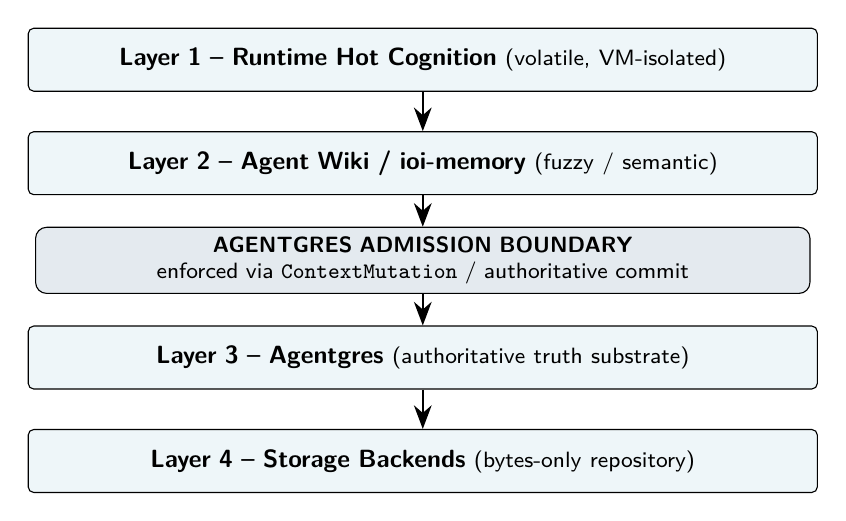
\begin{tikzpicture}[scale=1,transform shape,node distance=5mm and 9mm]
\node[ioibox,text width=96mm] (l1){\textbf{Layer 1 -- Runtime Hot Cognition} \footnotesize(volatile, VM-isolated)};
\node[ioibox,below=of l1,text width=96mm] (l2){\textbf{Layer 2 -- Agent Wiki / ioi-memory} \footnotesize(fuzzy / semantic)};
\node[draw,fill=ioikw!12,rounded corners,below=4mm of l2,text width=96mm,align=center,font=\sffamily\footnotesize](b){\textbf{AGENTGRES ADMISSION BOUNDARY}\\ enforced via \texttt{ContextMutation} / authoritative commit};
\node[ioibox,below=4mm of b,text width=96mm] (l3){\textbf{Layer 3 -- Agentgres} \footnotesize(authoritative truth substrate)};
\node[ioibox,below=of l3,text width=96mm] (l4){\textbf{Layer 4 -- Storage Backends} \footnotesize(bytes-only repository)};
\draw[ioiflow](l1)--(l2);\draw[ioiflow](l2)--(b);\draw[ioiflow](b)--(l3);\draw[ioiflow](l3)--(l4);
\end{tikzpicture}
\end{center}

While Agentgres manages admitted operational truth, \emph{ioi-memory}
manages the agent's private semantic memory, thread checkpoints, and
local context caches as adjacent runtime-memory material. Those
checkpoints and caches accelerate recall, enrichment, rollback, or
inspection; they do not replace Agentgres operation logs, ArtifactRefs,
projection checkpoints, restore validity, or replay authority. The
memory plane is organized as a modular, tiered architecture:

\begin{enumerate}
\def\labelenumi{\arabic{enumi}.}
\tightlist
\item
  \textbf{Thread Execution (LangGraph-shaped):} Maintains resumable
  transcripts and bounded working state.
\item
  \textbf{Tiered Ontology (Letta-shaped):} Separates memory into
  distinct \emph{working}, \emph{core}, and \emph{archival} layers.
\item
  \textbf{Background Enrichment (Zep-shaped):} Utilizes an asynchronous
  pipeline for summaries, entity extraction, and compaction, avoiding
  synchronous runtime bottlenecks.
\item
  \textbf{Local Evidence / Artifact Cache:} May cache or index
  blob-oriented evidence and artifact payloads for retrieval. Artifact
  identity, lifecycle, checkpoint refs, replay meaning, and restore
  validity remain Agentgres Artifact Plane concerns; storage backends
  hold bytes.
\end{enumerate}

\hypertarget{locality-by-default}{%
\subsubsection{3.6.1 Locality-by-Default}\label{locality-by-default}}

By default, the substrate index remains local:

\begin{enumerate}
\def\labelenumi{\arabic{enumi}.}
\tightlist
\item
  \textbf{Local execution:} Retrieval occurs against the local substrate
  and context is consumed locally.
\item
  \textbf{Remote execution:} When offloading to a provider, the runtime
  does not export the full corpus or index. It exports only a
  \textbf{task-scoped context slice} under the privacy-preserving
  injection protocol.
\end{enumerate}

Instead of moving user data to centralized compute, IOI moves the
compute to the data.

\textbf{Invariant:} the user's Agent Wiki / \emph{ioi-memory} corpus,
retrieval indexes, and durable workspace intelligence never become a
provider dependency. Provider runs receive only policy-bound context
slices, redacted projections, encrypted refs, or cTEE/private-workspace
handles.

\hypertarget{the-memory-api}{%
\subsubsection{3.6.2 The Memory API}\label{the-memory-api}}

Agent Wiki / \emph{ioi-memory} exposes a uniform, policy-governed
retrieval interface to agents and workflows. It utilizes
\textbf{Intent-Constrained Addressing (ICA)} to abstract over raw file
formats and storage locations, treating user context as a queryable
knowledge graph rather than a directory tree. Durable or
behavior-affecting updates still cross the Agentgres Admission Boundary
through \emph{ContextMutation} or equivalent Agentgres operations before
they become canonical, portable, or replay-relevant.

// Querying Agent Wiki / ioi-memory via ICA

agent.memory.query("Q3 financial reports", limit = 5)

The runtime resolves this into a policy-governed retrieval operation
against the local Agent Wiki / \emph{ioi-memory} plane and Agentgres
domain refs, returning the minimal set of relevant chunks (plus
metadata/provenance) required for the current step of the agent DAG.

\hypertarget{privacy-preserving-context-injection}{%
\subsubsection{3.6.3 Privacy-Preserving Context
Injection}\label{privacy-preserving-context-injection}}

When a local agent offloads to a provider, remote execution needs
context to be useful, but users require privacy by default. IOI solves
this with \textbf{privacy-preserving context injection}: a protocol that
minimizes the exported surface area, binds it to explicit policy, and
encrypts it under session-scoped keys.

The export follows the selected owner contract: a scoped MemoryProjection or
ContextLease for goal work, a ContextHandoff/TaskBriefPayload for delegation,
or a PrivateWorkspaceCapsule and custody profile for protected remote work.
No generic packet type is allowed to absorb memory truth, authority, or raw
workspace custody.

\hypertarget{portable-memory-vault-and-projection-contract}{%
\subsubsection{3.6.4 Portable Memory Vault and Projection
Contract}\label{portable-memory-vault-and-projection-contract}}

A \textbf{MemorySpace} is durable workspace/project/domain memory truth.
Harnesses and models consume scoped \textbf{MemoryProjections}; they do not
own the raw store, and harness-local memory remains cache. A run proposes a
durable addition, supersession, or archive operation through a
\textbf{ContextMutationEnvelope}. Review applies the same validation,
sensitivity, connector, provenance, policy, and Agentgres admission gates as
ordinary memory mutation and emits a context-mutation receipt.

OutcomeRoom state is not memory merely because a participant observed it.
Messages, attempts, findings, ontology mappings, evaluator suggestions,
leaderboard state, and ParticipantStateBundles remain provenance-bearing,
tainted collaboration inputs until the owning domain admits a specific
ContextMutation. Admission must preserve source and room refs, license and
export posture, evidence and assurance stage, contradiction or supersession,
retention, and any downstream recall obligation. Popularity, participant
consensus, a signature, or a receipt alone cannot promote room material into
durable memory, routing policy, an ontology, or production capability.

The portable \emph{ioi.hypervisor.memory-vault.v1} bundle is a
human-readable transport for MemorySpace records, memory entries, skills, and
automation affinities. It preserves stable refs, tags, source refs,
confidence, sensitivity, compatibility, expiry, archive/revoke state,
connector refs, timestamps, and structured sidecars. Export scrubs and
reports credential material; import rejects credential-bearing bundles,
validates records through the ordinary gates, remains idempotent, and reports
same-ID content conflicts rather than overwriting or duplicating silently.

The vault is a portable serialization of MemorySpace truth, not an independent
truth source or harness prompt file. Agentgres records admitted meaning and
mutations; encrypted storage or archive backends hold bytes; authority and
policy determine who may view, import, export, mutate, declassify, or restore.
The room-specific ParticipantStateBundle is a different portable object: it
preserves the participant's permitted work, contribution, evidence, receipt,
acceptance, settlement, and dispute lineage while excluding private room
database state, raw secrets, protected plaintext, unauthorized connector
payloads, unrelated memory, and non-opted-in training traces. Neither bundle
grants continuing room access or execution authority.

\hypertarget{domain-ontologies-and-data-recipes}{%
\subsection{3.7 Domain Ontologies and Data
Recipes}\label{domain-ontologies-and-data-recipes}}

Federated Domain Ontologies and Data Recipes are IOI's semantic world plane.
They make independently governed domains legible to workers without requiring
one global ontology or one global database. An ontology states what one
governed domain means under a namespaced, versioned contract; a Data Recipe
states how raw sources become ontology-bound runtime, training, evaluation,
and projection data.

A \emph{DomainOntology} defines entities, relationships, events, actions,
states, roles, invariants, namespace ownership, compatibility, and deprecation
policy. Its immutable \emph{OntologyVersion} and locally governed
\emph{OntologyOverlay} profiles preserve base-version lineage. A
\emph{CanonicalObjectModel} grounds that meaning in identifiers, schemas,
lifecycle states, constraints, privacy classes, authority needs, and
projection hints.

\textbf{Local canonicality is the default.} An organization or autonomous
system may canonically define its own objects, actions, assertions, and policy.
Cross-domain work declares namespaced versions, compatibility ranges,
crosswalks, mapping decisions, and policy-bound projections. No network-wide
ontology, crosswalk, or room schema silently overrides a domain's local
definition, and AIIP semantic negotiation does not become a universal schema
authority.

Operational admission and semantic truth remain distinct. A
\emph{ProvenanceAssertion}, represented by the shared
\emph{OntologyAssertion} envelope, records subject, predicate, value, valid and
transaction time, source and observation context, confidence or uncertainty,
supporting and contradicting evidence, applicability, causal or
counterfactual context where relevant, supersession, dispute, and admission
state. Agentgres can prove that a domain admitted that assertion under a
policy and evidence set; admission does not make the proposition universally
true.

Cross-domain meaning is explicit and challengeable. An
\emph{OntologyCrosswalk} is the \emph{OntologyMapping} profile that declares
source and target versions, mapped objects, relationships, events, and actions,
compatibility, loss, ambiguity, policy-bound views, validation, and migration.
A \emph{SemanticMappingDecision} applies a crosswalk or adapter to a concrete
handoff, query, object, or action and binds the target, decision maker,
verifier challenges, version, and decision receipt. Silent field equivalence
is forbidden.

Ontology actions become executable only through an
\emph{OntologyActionContract}. The contract binds the semantic action and
target object to typed inputs and outputs; preconditions, postconditions,
invariants, and expected state transition; runtime, tool, automation, and
\emph{prim:*} capability requirements; local policy and \emph{scope:*}
authority requirements; risk, approval, revocation, preview, and dry-run
posture; idempotency and retry behavior; one external-effect recovery class
(\texttt{replayable}, \texttt{checkpointable}, \texttt{compensatable},
\texttt{reconciliation\_required}, or \texttt{non\_retryable}); ambiguous-effect
reconciliation and compensation; verifier, evidence, and receipt obligations;
and a Physical Action Safety profile where an actuator can be affected. An
action name or connector method alone is never an execution contract.

Ontology semantics do not grant power. Local or domain governance and the
applicable authority provider authorize; the Hypervisor Daemon admits and
enforces execution; Agentgres admits resulting durable operational state. A
prior transformation or mapping receipt is evidence of that boundary event,
not perpetual permission to read, train, export, or act.

Data Recipes define how source systems become admitted semantic state. A
\emph{DataRecipe} maps documents, connector payloads, traces, work analytics,
feedback, examples, corrections, and source systems into ontology-bound
objects and assertions, policy-bound data views, evaluation datasets,
distilled ontology datasets, and Agentgres projections. Raw connector payloads
remain source material until a \emph{ConnectorMapping}, transformation,
validation, policy, and receipt path admits their meaning.

The canonical path is:

raw sources

-\textgreater{} ConnectorMapping

-\textgreater{} DataRecipe

-\textgreater{} TransformationRun

-\textgreater{} canonical ontology-bound objects

-\textgreater{} PolicyBoundDataView

-\textgreater{} DistilledOntologyDataset / EvaluationDataset /
WorkerTraining / OntologyProjection

-\textgreater{} WorkerManifest, MoW routing, service outcomes

Workers train on ontology-bound data, not raw blobs. For efficient
specialist workers, the best substrate is often \textbf{distilled
ontology-bound data}: compact examples, counterexamples, verifier
assertions, tool traces, canonical object transitions, rubric judgments,
and failure regressions derived from ontology-bound source material.

An ontology-bound OutcomeRoom may share a namespaced collaboration schema for
objectives, frontier items, claim leases, hypotheses, attempts, findings,
artifacts, evaluations, verifier challenges, resource leases, contribution
claims, and decisions. The declared hosted or federated policy admits the
shared-room projection; it does not merge participating Agentgres domains into
one mutable graph. Other domains receive only authorized projections, proofs,
summaries, derived objects, or query results.

Adoption is progressive. A domain may begin with the minimal consequential
objects and action contracts required for useful work, then learn and govern
new schemas, mappings, assertions, views, and evaluations from admitted work.
IOI does not require exhaustive enterprise modeling before a worker may act.

\hypertarget{canonical-object-models-and-connector-mappings}{%
\subsection{3.8 Canonical Object Models and Connector
Mappings}\label{canonical-object-models-and-connector-mappings}}

Connector payloads are not canonical domain truth by themselves. A
\emph{ConnectorMapping} maps provider fields, files, events, and actions
into canonical object models and authority scopes. For example, CRM
records, emails, spreadsheets, PDFs, repo events, tickets, and prior
work traces become domain objects only after a DataRecipe extracts,
redacts, normalizes, dedupes, validates, and links them under policy.

\hypertarget{distilled-ontology-datasets-and-evaluation-datasets}{%
\subsection{3.9 Distilled Ontology Datasets and Evaluation
Datasets}\label{distilled-ontology-datasets-and-evaluation-datasets}}

\emph{DistilledOntologyDataset} is a compact, high-signal dataset
derived from ontology-bound source truth. Distillation may use teacher
workers, verifier workers, deterministic gates, human reviewers, and
data recipes. It may reduce source volume, but it must not erase
provenance. A distilled dataset binds source commitments, recipe
versions, policy-bound data view refs, transformation receipts,
teacher/verifier refs when used, and rubric or benchmark bindings.

\emph{EvaluationDataset} is the benchmark-facing counterpart: golden
cases, holdouts, adversarial cases, failure regressions, expected
outputs, rubric refs, benchmark refs, and provenance commitments.
Evaluation datasets are not ad hoc folders of examples; they are
receipted inputs with domain meaning.

\hypertarget{network-routing-and-work-graphs}{%
\section{4. Network, Routing, and Work
Graphs}\label{network-routing-and-work-graphs}}

IOI replaces the flat gossip mesh of traditional blockchains with an
\textbf{Elastic Topology}: locality-first execution with network
escalation only when capacity, capabilities, or enforceability require
it.

\hypertarget{private-workspace-backed-by-ctee}{%
\subsection{4.1 Private Workspace Backed by
cTEE}\label{private-workspace-backed-by-ctee}}

\textbf{Implementation status: speculative.} This section defines the target
custody contract; no current cTEE implementation or no-plaintext-custody
product claim is implied.

Remote execution and workload offloading to untrusted or rented compute
nodes --- such as decentralized DePIN nodes or hosted third-party
virtual machines --- are governed strictly by the \textbf{Private
Workspace backed by cTEE} posture. A hostile-root node must never become
the plaintext custody domain for protected workspace state. Under this
posture, simple encryption-at-rest is insufficient, because the node's
memory could still expose raw workspace variables during live execution.
Instead, a conforming future runtime establishes a \textbf{Cryptographic Trusted
Execution Envelope (cTEE)} that enforces the declared
\textbf{no-plaintext-custody} profile for protected workspace assets. A
protected remote run remains a temporary
escalation from a Hypervisor Node runtime (Local) into a Provider runtime
(Session): the Hypervisor Node exports a minimal execution capsule, receives a
result plus verifiable accounting artifacts, and reintegrates the output
into the local agent graph --- but that capsule carries no plaintext
custody of protected state.

When the selected privacy posture is software-only, cTEE means
\textbf{zero-disclosure cryptographic partitioning}, not software-only
memory isolation. Protected state remains encrypted, secret-shared,
committed, guardian/client-held, or assembled locally through
candidate-lattice private decoding. The hostile-root provider may receive
public trunks, redacted projections, encrypted refs, candidate lattices,
and capability handles, but it MUST NOT receive the deciphering key or
materialize protected plaintext inside provider-visible CPU, GPU, disk,
log, cache, or process memory. Local lattice assembly, guardian
selection, cryptographic operators, or approved confidential-compute
lanes are the privacy mechanism; encrypting a normal plaintext runtime
is not.


\begin{center}
\needspace{6\baselineskip}
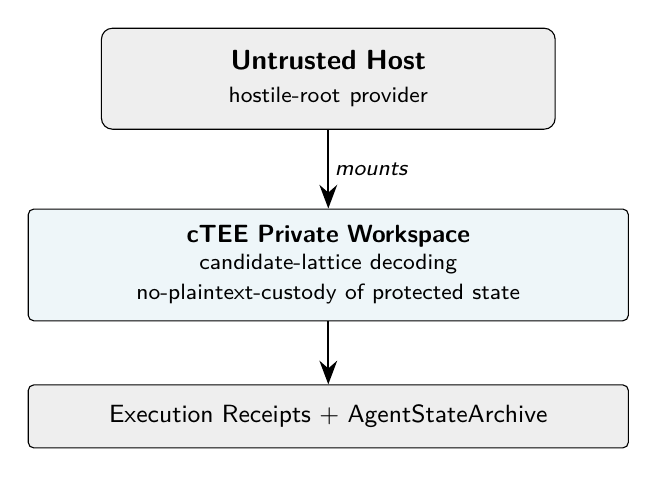
\begin{tikzpicture}[scale=1,transform shape,node distance=5mm and 10mm]
 % cTEE private workspace
\node[draw,rounded corners,fill=ioibg,inner sep=8pt,text width=52mm,align=center,font=\sffamily] (host){\textbf{Untrusted Host}\\\footnotesize hostile-root provider};
\node[ioibox,below=10mm of host,text width=72mm] (tee){\textbf{cTEE Private Workspace}\\\footnotesize candidate-lattice decoding\\ no-plaintext-custody of protected state};
\node[ioiplain,below=8mm of tee,text width=72mm] (rcpt){Execution Receipts + AgentStateArchive};
\draw[ioiflow](host)--node[ioilabel,right]{mounts}(tee);
\draw[ioiflow](tee)--(rcpt);
\end{tikzpicture}
\end{center}

The Offload mechanism targets a \textbf{Private-Execution Non-Exposure}
property. The exact guarantee depends on the selected substrate and must
be represented explicitly in the receipt bundle:

\begin{enumerate}
\def\labelenumi{\arabic{enumi}.}
\tightlist
\item
  \textbf{Provider exposure bound:} what the infrastructure operator can
  and cannot observe under the declared substrate threat model.
\item
  \textbf{User exposure bound:} what the user can and cannot extract
  from developer-owned logic, weights, or protected data.
\item
  \textbf{Developer exposure bound:} what the developer can and cannot
  observe about the user's private inputs or context slices.
\item
  \textbf{Verifier requirements:} which attestations, proofs,
  transcripts, commitments, or replay evidence are required before the
  output can be accepted.
\end{enumerate}

The protocol mandates a \textbf{Session Erasure Obligation}. A provider
must emit evidence that the session was closed, state was not retained
beyond the authorized window, and any cached context was deleted or
rendered cryptographically inaccessible according to the substrate's
erasure model. For TEE-backed sessions, this may include teardown
attestations and enclave lifecycle receipts. For cryptographic operator
paths, this may include proof transcripts, key-erasure commitments, MPC
transcript closure, or output-only commitments.

Session Offloading is strictly restricted to cognitive and data
operations. Offloading migrates only the declared runtime-session state
needed for the step. The wallet.network authority keys, policy engine,
kinetic operations (mouse, keyboard, hardware control), and local memory
substrate remain on the Hypervisor Node or authenticated client
authority domain.

To enable computation without exposing private state, the workflow is
split into public/compartmentalized execution payloads and secure local
state.

\textbf{Allowed Node Exposure (What the Node May Receive):}

-- Public trunk code and dependency blueprints.

-- Redacted projections and schema definitions.

-- Encrypted references and content-addressed commitments.

-- Candidate lattices (for structured output decoding).

-- Public model weights and benchmark kernels.

-- Sealed private-head handles and capability-exit requests.

\textbf{Protected State (What the Node Must Never Receive in
Plaintext):}

-- Protected user files, raw PII, and private research notes.

-- Proprietary quant strategy source, private thresholds, and private
coefficients.

-- Ambient API credentials and private memory indexes.

-- Live portfolio states and unredacted transaction ledger logs.


\begin{center}
\needspace{6\baselineskip}
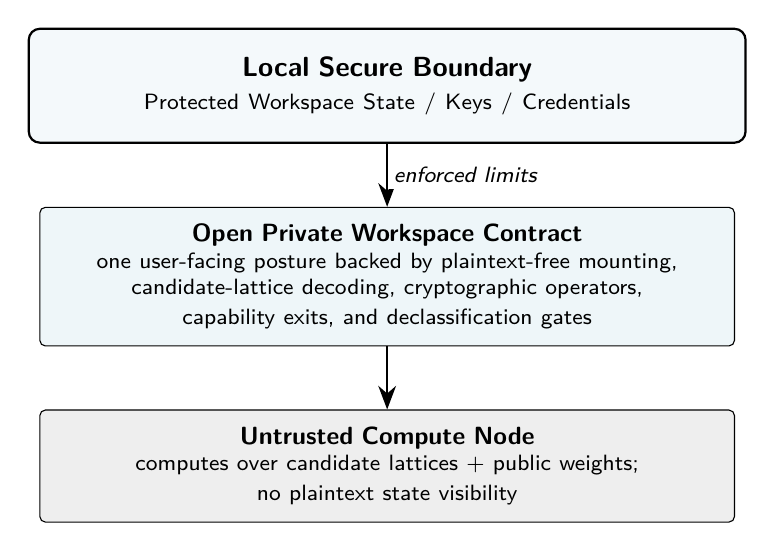
\begin{tikzpicture}[scale=1,transform shape,node distance=5mm and 10mm]
\node[draw,thick,rounded corners,fill=ioihead!25,inner sep=10pt,text width=84mm,align=center,font=\sffamily] (lb){\textbf{Local Secure Boundary}\\\footnotesize Protected Workspace State / Keys / Credentials};
\node[ioibox,below=8mm of lb,text width=84mm] (cm){\textbf{Open Private Workspace Contract}\\\footnotesize one user-facing posture backed by plaintext-free mounting,\\ candidate-lattice decoding, cryptographic operators,\\ capability exits, and declassification gates};
\node[ioiplain,below=8mm of cm,text width=84mm] (un){\textbf{Untrusted Compute Node}\\\footnotesize computes over candidate lattices + public weights;\\ no plaintext state visibility};
\draw[ioiflow](lb)--node[ioilabel,right]{enforced limits}(cm);
\draw[ioiflow](cm)--(un);
\end{tikzpicture}
\end{center}


\textbf{cTEE Mechanism Stack.} This is speculative target architecture; no
current cTEE implementation or no-plaintext-custody product claim is implied.
The target user-facing posture is singular:
\textbf{Open Private Workspace}. The user does not choose between
cryptographic modes during ordinary work. The \textbf{Hypervisor Daemon}
would realize that posture through a mechanism stack selected by policy,
cost, risk, and workload fit:

1. \textbf{Plaintext-Free Runtime Mounting:} Workspaces are mounted as
virtual crypt-volumes. The host file system cannot access file
structures, directory names, or raw bytes. This protects workspace
custody---not proprietary model weights. Defending weights requires a
separate \textbf{ModelWeightCustodyProfile}: local/customer custody,
provider API custody, accepted TEE/customer-cloud custody,
cryptographic-operator partitioning, or an explicitly receipted
provider-trust route. Any no-plaintext model-mount path must be verified
under that weight-custody profile; it is not implied by workspace cTEE.

2. \textbf{Candidate-Lattice Private Decoding:} The target default
high-throughput profile. The remote node generates structured candidate
token trees (lattices) using public base weights; the final private
selection and token assembly are resolved locally or within a secure
boundary. The \textbf{CandidateCoverageProfile} declares candidate count,
coverage assumptions, public-token overhead, and the expected
selection-leakage surface for the protected task.

3. \textbf{Counterfactual Lattice Execution:} Used where zero online
selection leakage is mandated. The node computes multiple counterfactual
execution paths simultaneously, obfuscating the actual logical branch
taken under the declared leakage profile; it is not a claim that all
semantic inference, timing, or side-channel leakage disappears.

4. \textbf{Cryptographic Operator Plane:} FHE, MPC, garbled-circuit,
ORAM, local/client guardian, browser/phone guardian, wallet.network, or
enterprise-key-service mediated operators for private heads, private
model scoring, policy checks, and private retrieval. This plane may use
one authenticated access point or a threshold path when the workload
requires stronger non-collusion assumptions.

5. \textbf{Capability Exits \& Declassification Gates:} Managed channels
that intercept action attempts at their declared control points.
Actions must be packaged as capability-exit requests and passed through
a local declassification gate before execution.

The daemon binds each protected offload to an
\textbf{ExecutionPrivacyPosture}, a \textbf{CustodyProof}, and, when the
agent is allowed to run beyond the immediate user session, an
\textbf{AutonomyLease}. The \textbf{PrivateAgencyTransform} rewrites
candidate-selection-reducible work into public/generic generation plus
private selection, scoring, policy, or declassification, preserving the
no-plaintext-custody invariant while keeping the rented node useful for
high-throughput public kernels.

\textbf{Privacy Posture Comparison.}

\begin{longtable}[]{@{}
  >{\raggedright\arraybackslash}p{(\linewidth - 8\tabcolsep) * \real{0.2000}}
  >{\raggedright\arraybackslash}p{(\linewidth - 8\tabcolsep) * \real{0.2000}}
  >{\raggedright\arraybackslash}p{(\linewidth - 8\tabcolsep) * \real{0.2000}}
  >{\raggedright\arraybackslash}p{(\linewidth - 8\tabcolsep) * \real{0.2000}}
  >{\raggedright\arraybackslash}p{(\linewidth - 8\tabcolsep) * \real{0.2000}}@{}}
\toprule\noalign{}
& & & & \\
\midrule\noalign{}
\endhead
\bottomrule\noalign{}
\endlastfoot
Posture / Path & Trust Assumptions & Custody Model & Performance
Characteristics & Primary Exposure Bounds \\
\textbf{Plaintext Workspace} & Absolute trust in host root and
infrastructure provider. & Host retains full plaintext custody of memory
and storage. & Full bare-metal hardware speed. & Total exposure.
Host-root has full visibility into all keys, files, and variables. \\
\textbf{cTEE Private Workspace} & Zero trust in host for protected
workspace plaintext under the declared leakage profile. & Host receives
no protected plaintext by design; it computes over public trunks,
redacted projections, encrypted refs, candidate lattices, and capability
handles. & Near-native for public/generic trunks; extra cost depends on candidate overgeneration,
private-head routing, and crypto-operator use. & Constrained by explicit
leakage profiles, declassification gates, custody proofs, and deterrence
metrics. \\
\textbf{Cryptographic Operator Path} & Mathematical hardness guarantees
(FHE/MPC). & Zero plaintext custody. Mathematical guarantees independent
of hardware. & High compute overhead; restricted to low-dimensional
linear algebra (private heads, scores). & Bound by mathematical security
parameter bounds (e.g., LWE hardness). \\
\textbf{Confidential GPU / Hardware TEE Path} & Hardware vendor trust
(Intel, AMD, NVIDIA). & Hardware-enforced memory isolation from host OS.
& High performance, near native CPU/GPU execution. & Vulnerable to
side-channel analysis and hardware-level root-key exploits. \\
\textbf{Provider API Path} & Trust in third-party API provider (OpenAI,
Anthropic). & Plaintext custody is transferred entirely to the API
provider. & Zero local compute footprint; fast network transit. &
Provider-readable plaintext visibility into sensitive context supplied
to the API host. \\
\end{longtable}

\hypertarget{trigger-conditions}{%
\subsubsection{4.1.1 Trigger conditions}\label{trigger-conditions}}

Hypervisor Core, the Workflow Compositor, or the selected HarnessProfile
MAY propose an offload when any of the following
holds:

\begin{enumerate}
\def\labelenumi{\arabic{enumi}.}
\tightlist
\item
  \textbf{Capacity limit:} Local hardware cannot satisfy the declared
  execution requirements (e.g., model snapshot exceeds VRAM, missing
  accelerator class).
\item
  \textbf{Capability gap:} The task requires a tool or dataset not
  available locally (e.g., enterprise data feed, specialized service,
  regulated connector).
\end{enumerate}

\hypertarget{the-hybrid-data-plane-dual-path-io}{%
\subsubsection{4.1.2 The Hybrid Data Plane (Dual-Path
I/O)}\label{the-hybrid-data-plane-dual-path-io}}

The Hypervisor Daemon selects the transport based on the topology of the
agent work graph and the approved provider/session policy:

\textbf{Remote path:} The selected provider, harness, connector, or private-
workspace contract declares its authenticated transport and the exact refs or
context projection it may carry. Transport encryption protects transit; it
does not by itself make the destination private. Plaintext exposure remains a
property of the declared cTEE/private-workspace, TEE/confidential-compute,
customer-controlled, redacted-only, or provider-trust posture.

\textbf{Local path:} Co-located runtimes may use shared memory, local sockets,
or other zero-copy/IPC optimizations when supported. These are implementation
choices beneath the same typed contracts and do not change authority,
privacy, receipt, or admission semantics.

\hypertarget{session-bootstrap-routing-and-route-selection}{%
\subsubsection{4.1.3 Session bootstrap: Routing and Route
Selection}\label{session-bootstrap-routing-and-route-selection}}

Hypervisor presents four user choices rather than exposing provider-market
mechanics as the product model:

\begin{itemize}
\tightlist
\item
  \textbf{Run local} on the user's machine or HypervisorOS node.
\item
  \textbf{Use my infrastructure} through a connected provider account,
  customer cluster, bare-metal/SSH target, or enterprise environment.
\item
  \textbf{Pick a cloud} by selecting a specific provider or venue.
\item
  \textbf{Let Hypervisor choose} under explicit cost, custody, region,
  reliability, failover, and receipt constraints.
\end{itemize}

Under those choices are three placement sources: \textbf{connected}
infrastructure billed to the user, \textbf{managed} capacity where IOI or
a partner is provider-of-record, and \textbf{optimized} placement where
Hypervisor compares, procures, fails over, reconciles, or aggregates routes.
\emph{decentralized.cloud} may supply resource-intelligence candidates to the
optimized path, but it is neither mandatory nor the provider-account, VM
lifecycle, credential, spend-authority, storage-custody, restore-truth, or
execution owner.

A \textbf{CloudResourceIntent} or equivalent placement request produces
evidence-bound \textbf{CloudResourceCandidates}, provider quotes, custody
plans, failover plans, and spend estimates. Hypervisor selects a candidate
into its own \textbf{PlacementDecision}. Provider credentials remain in a
\textbf{ProviderCredentialBinding} under wallet.network or approved
customer authority; agents receive scoped leases rather than raw keys.
Provider lifecycle work executes through the appropriate adapter and emits
\textbf{ProviderOperationReceipts}, \textbf{SpendReceipts}, snapshot/archive
refs, and restore evidence admitted by Agentgres.

Direct and BYO adapters do not universally require the remote target to run
a Hypervisor Daemon or hardware attestation. The adapter must preserve its
real provider semantics and satisfy the declared readiness, authority,
privacy, evidence, and receipt contract. A remote daemon handshake applies
when the selected runtime profile actually includes a daemon-compatible node;
ordinary SSH, cloud, storage, DePIN, or customer-provider adapters use their
own conformance path.

The Handshake \& Topology Negotiation

Once a route is selected, Hypervisor performs the readiness or handshake
protocol appropriate to that adapter and runtime profile:

\textbf{Security Verification:} The Hypervisor Node verifies that the
destination satisfies the declared posture before transmitting data or
refs. Public work may run on ordinary provider lanes. Private workspace
state requires cTEE/private-workspace constraints, hardware confidential
compute, customer-controlled infrastructure, cryptographic private
operators, or explicit provider-trust approval depending on policy.

\textbf{Topology Negotiation:} The runtime negotiates data and context
boundaries. Simple steps use a task-scoped context slice. Goal-shaped or
delegated work uses ContextCells, ContextLeases, and typed ContextHandoffs
with explicit result, blocker, evidence, and continuation payloads. It does
not rely on shared-memory CRDTs or copied agent chat as the durable merge
contract.

The user retains control over the placement choice and can inspect the
candidate evidence, selected PlacementDecision, fee basis, privacy posture,
and receipts. Adapter-specific bootstrapping varies; the authority, evidence,
and truth boundaries do not.

\hypertarget{typed-provider-handoff-and-private-workspace-capsules}{%
\subsubsection{4.1.4 Typed Provider Handoff and Private-Workspace
Capsules}\label{typed-provider-handoff-and-private-workspace-capsules}}

IOI does not define one universal \emph{OffloadPacket}. A placement decision
selects an adapter and the narrow owner contract appropriate to the work:

\begin{itemize}
\tightlist
\item
  Goal-shaped delegated work crosses a \textbf{ContextHandoff} carrying a
  \textbf{TaskBriefPayload}, then a \textbf{HarnessInvocation}; the generic
  result returns as a \textbf{WorkResult} and may propose an
  \textbf{OutcomeDelta}, with verifier and continuation refs.
  \textbf{ImplementationResultPayload} is only the software-work profile for
  files, patches, diffs, tests, and implementation summaries.
\item
  Tool, connector, and MCP work binds to a \textbf{RuntimeToolContract} or
  declared surface MCP contract and its primitive, authority, risk, privacy,
  budget, and receipt requirements.
\item
  Protected remote work uses a \textbf{PrivateWorkspaceCapsule} bound to an
  \textbf{ExecutionPrivacyPosture}, \textbf{CustodyProof}, leakage profile,
  model-weight custody posture, and, when offline autonomy is authorized, an
  expiring \textbf{AutonomyLease}.
\item
  Provider lifecycle work binds the \textbf{ProviderAccount},
  \textbf{ProviderCredentialBinding}, \textbf{RuntimeNode},
  \textbf{PlacementDecision}, and relevant snapshot, restore, spend, and
  provider-operation refs.
\end{itemize}

Every handoff is minimized to the context, artifacts, capabilities, and
authority required by its declared contract. wallet.network root material,
ambient provider credentials, and unbounded workspace state never become
generic handoff payloads. Transport encryption protects transit; it does not
upgrade the destination's custody or privacy posture.

\hypertarget{provider-execution-admission-and-reintegration}{%
\subsubsection{4.1.5 Provider Execution, Admission, and
Reintegration}\label{provider-execution-admission-and-reintegration}}

Before dispatch, Hypervisor evaluates adapter readiness, budget, privacy,
custody, policy, and current authority. Provider mutations are performed by the
daemon through the selected adapter under scoped credential and capability
leases; agents do not receive raw provider secrets.

Provider-native ids, statuses, snapshots, bills, and success claims return as
evidence. They become operational or restore truth only after the daemon and
Agentgres validate and admit the applicable hashes, state roots, receipts, and
owner contracts. \textbf{ProviderOperationReceipt} and \textbf{SpendReceipt}
records cover successful and refused crossings; private work additionally
carries the evidence required by its \textbf{CustodyProof} and selected
\textbf{VerifierPath}.

A returned artifact, plan, model output, or staged effect is therefore
pre-canonical. The receiving gate validates its signature and bindings,
normalizes the observation, runs required deterministic checks, and either
admits, rejects, or escalates it. Any effect materialized after a delay,
replay, or branch merge is re-authorized against the current revocation epoch,
grant expiry, and policy hash and mints new receipts. Failed verification
cannot be repaired by silently reusing the old grant; it begins a new proposal
or remains blocked.

\textbf{Implementation status.} Direct provider and BYO-provider lanes are
mixed and adapter-specific. Private Workspace backed by cTEE, including its
no-provider-trust mechanisms, remains speculative architecture; product
surfaces must not present that posture as implemented without the required
custody proof.
\hypertarget{session-accounting-and-value-flow}{%
\subsection{4.2 Session Accounting and Value
Flow}\label{session-accounting-and-value-flow}}

A Hypervisor Session or WorkRun may consume local resources, customer-billed
provider capacity, managed capacity, marketplace labor, connectors, storage,
verification, or public settlement. The accounting contract follows the owner
of each cost rather than imposing a universal state channel or packet format.

\textbf{Work Credits} are the product-wide usage and budget abstraction for
managed autonomous work. They may meter or budget model calls, runtime time,
provider operations, private managed execution, storage, Foundry jobs,
marketplace invocations, and other managed costs. They are not necessarily a
protocol token, payout asset, provider payment rail, or IOI L1 settlement
asset.

For provider operations, budget discovery precedes mutation. wallet.network or
the applicable local/domain authority approves the spend and credential use;
the daemon executes the provider call; \textbf{SpendReceipt} and
\textbf{ProviderOperationReceipt} records disclose the applicable cost,
credential source, grant, and outcome; Agentgres admits the operational
record. Customer-borne provider billing, IOI-managed billing, enterprise
invoicing, subscriptions, prepaid balances, and marketplace escrow may coexist
without changing that authority and truth ordering.

Payment, payout, and public settlement are separate rails. Local work-credit
debits and routine provider accounting remain local/domain records. A future
IOI L1 receives only selected public or economic commitments when escrow,
rights, licensing, reputation, dispute, cross-domain finality, or another
declared trigger requires it. No model call, tool call, Agentgres write,
authority check, local receipt, or self-hosted action incurs a protocol toll
merely because the substrate observed or proved it.

\textbf{Implementation status.} Fee-basis declarations and provider-resource
metering exist in parts of the current runtime. Work Credits, marketplace
fees, and token or BME settlement are planned or deferred, and IOI L1 has no
current deployment. Exact billing, escrow, and settlement schemas remain with
their product, wallet.network, marketplace, provider, and L1 owners.
\hypertarget{aiip-the-inter-autonomous-system-protocol}{%
\subsection{4.3 AIIP: The Inter-Autonomous-System
Protocol}\label{aiip-the-inter-autonomous-system-protocol}}

\textbf{AIIP is the Inter-Autonomous-System Protocol}: IOI's RPC-shaped,
semantic, receipt-native interoperability protocol for bounded autonomous
work and collaborative pursuit.

AIIP is not a lookup directory, a name-resolution service, a shared prompt
bus, or a global room database. It moves delegated work,
collaborative-pursuit updates, negotiated ontology and action profiles,
authority leases, receipt commitments, delivery and acceptance state,
settlement intents, reputation queries, dispute notices, and handoff finality
across bounded execution domains: local microharnesses, installed workers,
marketplace workers, outcome services, robot fleets, enterprise runtimes, and
peer autonomous systems. Each domain retains its runtime, private context, and
operational truth.

Short form:

\begin{center}
\emph{AIIP moves autonomous work across systems. IOI settles what
happened.}
\end{center}

The \emph{ai://} identifier grammar may be used for manifests, worker
packages, services, or system endpoints, but name resolution is only one
input to AIIP. The protocol itself is the signed, sequenced,
receipt-aware packet layer that lets bounded execution domains talk.

The layer boundary is:

\begin{itemize}
\tightlist
\item
  \textbf{Execution:} local runtimes, microharnesses, workers, APIs, robots,
  VMs, tools, and enterprise systems.
\item
  \textbf{Interop:} AIIP packets, profiles, channels, semantic mappings,
  restricted views, authority refs, receipt obligations, and settlement
  intents.
\item
  \textbf{Settlement:} selected IOI L1 roots, rights, escrows, disputes,
  reputation, and handoff finality when public or economic trust requires it.
\end{itemize}

The chain does not execute ordinary cognition or collaboration. A signed
packet makes a claim attributable and ordered; it does not make the claim
correct or accepted.

\textbf{AIIP does not grant execution authority.} AIIP packets convey
intentions, task contexts, receipt obligations, and structural payloads.
While an AIIP packet may reference requested primitive capabilities,
authority scopes, policy hashes, and settlement terms, the receiving
bounded execution domain must validate those claims against its own
policy, authority, and daemon gates. Authoritative execution permissions and
decryption leases are never granted by the interop packet itself. Local or
domain policy and the applicable authority provider authorize; the receiving
daemon admits and enforces work, mediates or executes effects, emits receipts,
and orchestrates replay; the receiving Agentgres domain admits durable
operational state.

The same semantic protocol is used in different modes. Hypervisor may
use AIIP semantics internally for local microharness routing over
in-process calls, Unix sockets, local HTTP, gRPC, JSON-RPC, NATS, or a
daemon bus. External handoffs use signed envelopes, authority leases,
receipt obligations, payment or escrow terms, reputation updates,
dispute windows, and mainnet commitments when consequential. Same
semantic protocol, different transport and settlement mode.

The canonical AIIP object model distinguishes the transport binding from
the work boundary. An \textbf{AIIPProfile} declares supported protocol
features, transports, receipt obligations, settlement modes, authority planes,
and payload classes. An \textbf{AIIPChannel} binds bounded execution domains
with ordering, replay protection, schema version, privacy posture, lease refs,
and dispute windows. A \textbf{BoundedExecutionDomain} declares its manifest,
capabilities, policy root, authority requirements, receipt schemas, state
boundary, runtime profile, settlement behavior, and supported AIIP profiles.

The field-level \textbf{AIIPEnvelope} in the common-envelope owner is the
normative superset. No application or protocol profile may publish a reduced
competing envelope. It preserves packet and payload identity while binding:

\begin{itemize}
\tightlist
\item
  message type, sender, recipient, channel, schema version,
  sequence-or-nonce, timestamp, and signature;
\item
  idempotency, causation, and correlation refs;
\item
  local, installed-worker, marketplace-worker, outcome-service,
  autonomous-system, collaborative-pursuit, and enterprise profiles;
\item
  policy and authority refs, MultiPartyCollaboration and OutcomeRoom refs,
  ontology, semantic-mapping, and action-schema profiles, restricted views,
  and verifier challenges;
\item
  payload hash and ref, receipt obligations, verifier and acceptor refs,
  settlement terms, and assurance stage; and
\item
  external-effect recovery class.
\end{itemize}

Payload bodies may remain private, encrypted, redacted, or available only to
authorized dispute participants. Public settlement anchors commitments and
roots rather than raw operational context.

AIIP preserves the assurance ladder rather than collapsing it into a
\texttt{verified} flag:

\begin{center}
receipt / attestation $\rightarrow$ evidence bundle $\rightarrow$
verification $\rightarrow$ acceptance $\rightarrow$ adjudication
$\rightarrow$ settlement
\end{center}

A receipt is an authenticated statement about its declared boundary fact. An
evidence bundle supports a claim. Verification means a named verifier applied
a named rule and version. Acceptance belongs to the user, customer, domain, or
counterparty. Adjudication resolves a challenge under policy. Settlement moves
rights or value under an accepted or adjudicated claim. Later stages do not
arise merely because an earlier receipt exists.

Every AIIP task or action profile that can create an external effect declares
one recovery class: \texttt{replayable}, \texttt{checkpointable},
\texttt{compensatable}, \texttt{reconciliation\_required}, or
\texttt{non\_retryable}. Restoring a channel, worker, VM, or environment does
not prove that the business or physical outcome was restored. A timeout after
dispatch follows the declared reconciliation policy; an unknown effect is not
blindly replayed, and compensation is a separately authorized action with its
own receipts.


\begin{center}
\needspace{6\baselineskip}
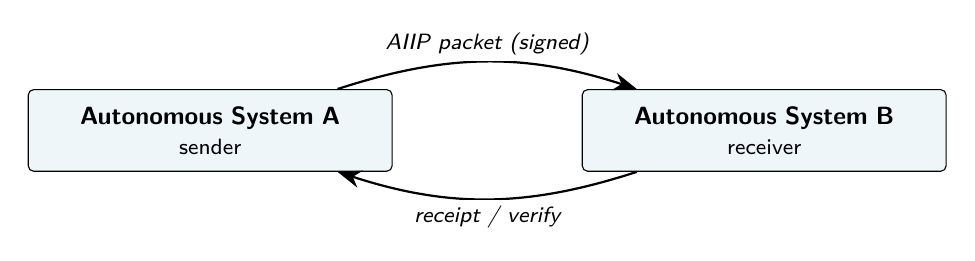
\begin{tikzpicture}[scale=1,transform shape,node distance=5mm and 10mm]
 % AIIP inter-autonomous-system
\node[ioibox,text width=42mm] (a){\textbf{Autonomous System A}\\\footnotesize sender};
\node[ioibox,right=24mm of a,text width=42mm] (b){\textbf{Autonomous System B}\\\footnotesize receiver};
\draw[ioiflow](a) to[bend left=18] node[ioilabel,above]{AIIP packet (signed)} (b);
\draw[ioiflow](b) to[bend left=18] node[ioilabel,below]{receipt / verify} (a);
\end{tikzpicture}
\end{center}


\textbf{AIIP packet classes.} The common envelope carries typed packet bodies
rather than undifferentiated bytes:

\begin{longtable}[]{@{}
  >{\raggedright\arraybackslash}p{(\linewidth - 4\tabcolsep) * \real{0.3333}}
  >{\raggedright\arraybackslash}p{(\linewidth - 4\tabcolsep) * \real{0.3333}}
  >{\raggedright\arraybackslash}p{(\linewidth - 4\tabcolsep) * \real{0.3333}}@{}}
\toprule\noalign{}
& & \\
\midrule\noalign{}
\endhead
\bottomrule\noalign{}
\endlastfoot
Packet & Meaning & Required posture \\
\emph{CapabilityDiscovery} & Discover a system, Worker, module, resource,
or capability. & Signed profile and eligibility refs. \\
\emph{TaskOffer / TaskAcceptance / Handoff} & Offer, accept, counteroffer,
or transfer bounded work. & Constraints, quote or SLA, authority, receipts,
and settlement posture. \\
\emph{SemanticProfileNegotiation} & Negotiate ontology and action-schema
versions, crosswalks or adapters, mapping loss or ambiguity, policy-bound
views, and verifier obligations. & Explicit, challengeable mapping decision. \\
\emph{OutcomeRoomDiscovery} & Query or publish a signed public or
permissioned objective, category, semantic and capability requirements,
eligibility, privacy, budget, verifier, settlement, and admission endpoint. &
No raw private room context. \\
\emph{RoomParticipation} & Request, admit, update, suspend, retire, or revoke
a participant lease and export permitted participant state. & Declared hosted
or federated admission owner. \\
\emph{FrontierUpdate / WorkClaim} & Propose or admit frontier state, or
claim, renew, release, expire, reassign, or quarantine bounded work. & Context,
authority, resource, data, tool, and budget lease refs. \\
\emph{AttemptFinding} & Publish positive, negative, inconclusive, invalid,
exploit-found, or superseded attempt and finding refs. & Method, lineage,
evidence, cost, reproduction, license, and disclosure posture. \\
\emph{VerifierChallenge / RoomAdmission} & Challenge a metric, rule,
verifier, evidence, mapping, eligibility, independence, or result; then
propose, admit, reject, supersede, or reconcile a WorkResult or OutcomeDelta. &
Versioned rules, affected work, and named admission path. \\
\emph{AuthorityQuery / AuthorityGrant} & Query or carry a bounded authority
lease reference. & Scope, subject, time, budget, policy, and receiver-side
validation. \\
\emph{ReceiptCommitment} & Commit to declared work-boundary facts. & Receipt
root or inclusion proof for later evidence and challenge. \\
\emph{DeliveryUpdate / AcceptanceDecision} & Record milestone, partial,
final, revision, cancellation, acceptance, rejection, or dispute-open state. &
Artifacts, evidence, criteria, and receipt roots. \\
\emph{SettlementIntent / Dispute / DisputeResolution / ReputationQuery} &
Request economic or reputation handling, challenge a claim, resolve a dispute,
or query contextual reputation. & Declared policy, evidence, window, and
remedy. \\
\end{longtable}

The Collaborative Pursuit profile applies these packet classes to an
OutcomeRoom above bounded GoalRuns. \texttt{hosted\_admission} names one
governed sequencing and admission domain and is the first conformance target.
\texttt{federated\_admission} names a versioned ordering, merge, quorum or
adjudication, conflict, failover, and recovery policy and is opt-in. Discovery
grants no membership, authority, budget, or data access. Admission creates a
RoomParticipantLease only after the named path accepts the typed request and
evidence. Exit releases or reassigns claims and can carry a signed,
policy-filtered ParticipantStateBundle. Hosted and federated rooms use the
same discovery, request, lease, exit, and export contracts; they differ in the
declared admission owner and watermark.

Participant packets are hostile input. Provenance, taint, license and export,
affiliation, independence, and trust labels survive transport. Room admission
must enforce rate, resource, spend, context, authority, privacy, quarantine,
anti-Sybil, anti-collusion, backpressure, and fair-allocation policy. Messages,
artifacts, mappings, evaluator suggestions, and consensus do not automatically
enter durable memory, ontology, routing policy, authority, production state,
or settlement.

\hypertarget{the-aiip-uri-scheme}{%
\subsubsection{4.3.1 The AIIP URI Scheme}\label{the-aiip-uri-scheme}}

ai://\textless authority\textgreater/\textless agent\_id\textgreater/\textless version\textgreater{[}?query{]}

\begin{itemize}
\tightlist
\item
  \textbf{Authority:} \emph{did:ioi:...} (public key, DAO address, or
  governance identity).
\item
  \textbf{Agent ID:} human-readable label (e.g.,
  \emph{personal-finance}).
\item
  \textbf{Version: }immutable release identifier (e.g.,
  \emph{sha256:...} or semantic version mapped to a content hash).
\end{itemize}

\hypertarget{resolution-result}{%
\subsubsection{4.3.2 Resolution Result}\label{resolution-result}}

Resolving an AIIP URI returns a structured Resolution Result:

\begin{itemize}
\tightlist
\item
  A content-addressed \textbf{Agent Manifest} (signed by authority).
\item
  An optional \textbf{Local Installation Handle} (if the package is
  already present in the local package inventory and indexed by Agent
  Wiki / \emph{ioi-memory}).
\item
  Zero or more candidate \textbf{Endpoints }(p2p, https, or
  driver-specific transports), ordered by trust policy and locality.
\item
  A declared \textbf{Primitive Capabilities and Authority Scopes
  requirement} for user review.
\item
  Optional \textbf{MoW routing metadata}, when present:
  \emph{sparse\_worker\_category}, \emph{benchmark\_profile\_refs},
  current leaderboard position or reputation root reference,
  \emph{routing\_eligibility\_status}, contribution terms, and
  \emph{training\_lineage\_ref}.
\end{itemize}

\hypertarget{resolution-logic-split-horizon-discovery}{%
\subsubsection{4.3.3 Resolution Logic: Split-Horizon
Discovery}\label{resolution-logic-split-horizon-discovery}}

When the runtime encounters an AIIP URI, it follows a deterministic
waterfall to prevent the ``DNS Leak'' problem where looking up an agent
reveals user intent:\\

Step 1: Local Install Cache (``Hosts File'')

\begin{itemize}
\item
  The runtime checks local package inventory, Agent Wiki /
  \emph{ioi-memory} indexes, and Agentgres admission refs.
\item
  If installed, it returns the local package handle (content hash /
  bundle ID) and skips network lookup.
\item
  \textbf{Latency:} \textasciitilde0ms. \textbf{Privacy:} Maximal.
\end{itemize}

Step 2: Pinned Registries (``Known
Good'')\protect\hypertarget{anchor}{}{}

\begin{itemize}
\item
  The Runtime checks a locally pinned list of trusted registries or
  providers (e.g., enterprise catalogs, user favorites) via encrypted
  transport.
\item
  If found, it returns the manifest and endpoints from the pinned
  source.
\item
  \textbf{Latency:} Low. \textbf{Trust:} Explicit.
\end{itemize}

Step 3: Network Discovery (``Dark Pool'')

\begin{itemize}
\item
  If not found locally, the Runtime may use privacy-preserving discovery
  methods such as \textbf{Oblivious Resolution} (e.g., PIR) to query
  registry or catalog endpoints without broadcasting the user's full
  intent.
\item
  Providers can operate in \textbf{Dark Pool Mode}, where capacity is
  not broadcast globally.
\end{itemize}

The Tower of Babel Solution: Federated Semantic Negotiation

To ensure that a ``Downloaded Accountant'' can speak to a ``Downloaded
Bank'', each domain declares namespaced ontology and action-schema profiles;
IOI does not assume one global schema registry. AIIP negotiates compatible
versions, explicit OntologyCrosswalk or adapter refs, lossy or unmapped fields,
restricted views, and verifier obligations. A challengeable
SemanticMappingDecision binds the mapping actually applied. The Hypervisor
Daemon validates the resolved typed action contract at admission, while local
or domain governance and the applicable authority provider authorize any
monetary or other consequential power.

\begin{itemize}
\tightlist
\item
  \textbf{Schema Enforcement:} A Worker Manifest MUST declare its I/O
  schemas (e.g., \emph{\emph{input: std:finance:invoice\_v1}},
  \emph{\emph{output: std:finance:tax\_report\_v2}}).
\item
  \textbf{Handshake:} Before work or value moves, the receiving domain
  verifies exact compatibility or admits an explicit mapping decision with
  its loss, ambiguity, policy-bound view, and verifier posture. This prevents
  ``semantic mismatch'' errors without silently making either domain's schema
  universal.
\end{itemize}

\hypertarget{the-worker-manifest}{%
\subsubsection{4.3.4 The Worker Manifest}\label{the-worker-manifest}}

The Worker Manifest is the declarative contract for execution. It
specifies what the agent is, what it requires, and where it can run.
These specifications make no vertical-specific architectural
assumptions: domain schemas are client-defined ontology packages
registered on aiagent.xyz, not hardcoded into the core engine.

A Worker Manifest MAY additionally declare MoW routing metadata:
\emph{sparse\_worker\_category}, \emph{benchmark\_profile\_refs},
\emph{evaluation\_rubric\_ref}, \emph{routing\_eligibility\_status},
\emph{contribution\_policy}, \emph{training\_lineage\_ref}, and
\emph{supported\_execution\_axes}.

Optional MoW routing fields:

\{

~~``sparse\_worker\_category'': ``std:code:rust\_security\_audit.v1'',

\begin{lstlisting}[language=rustioi]
  "benchmark_profile_refs": [
    "benchmark://ioi/categories/rust_security_audit/v1"
\end{lstlisting}
~~{]},

~~``evaluation\_rubric\_ref'':
``rubric://ioi/rust\_security\_audit/v1'',

~~``routing\_eligibility\_status'': ``eligible'',

~~``training\_lineage'': \{

\begin{lstlisting}[language=rustioi]
    "training_run_ref": "run://...",
    "dataset_commitment": "hash://...",
    "evaluation_receipt_root": "hash://..."
~~\},
\end{lstlisting}

~~``contribution\_policy\_ref'': ``policy://contribution/...'',

~~``license\_ref'': ``license://...''

\}


\begin{center}
\needspace{6\baselineskip}
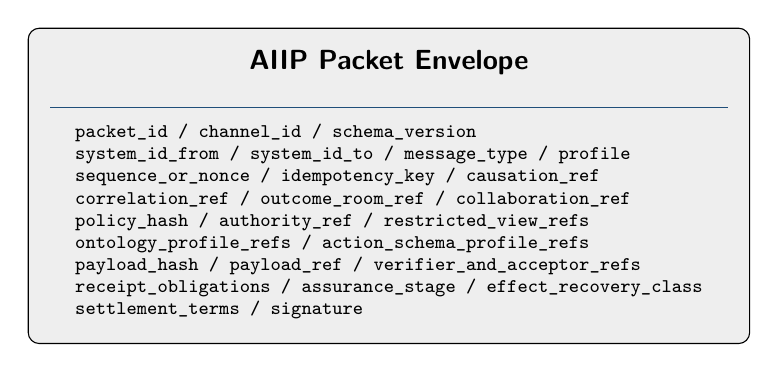
\begin{tikzpicture}[scale=1,transform shape,node distance=5mm and 10mm]
\node[draw,rounded corners,fill=ioibg,inner sep=8pt]{%
\begin{minipage}{86mm}
\centering{\sffamily\bfseries AIIP Packet Envelope}\par\vskip2pt
{\color{ioikw}\rule{\linewidth}{0.4pt}}\par\vskip4pt
{\ttfamily\scriptsize\begin{tabular}{@{}l@{}}
packet\_id / channel\_id / schema\_version\\
system\_id\_from / system\_id\_to / message\_type / profile\\
sequence\_or\_nonce / idempotency\_key / causation\_ref\\
correlation\_ref / outcome\_room\_ref / collaboration\_ref\\
policy\_hash / authority\_ref / restricted\_view\_refs\\
ontology\_profile\_refs / action\_schema\_profile\_refs\\
payload\_hash / payload\_ref / verifier\_and\_acceptor\_refs\\
receipt\_obligations / assurance\_stage / effect\_recovery\_class\\
settlement\_terms / signature
\end{tabular}}
\end{minipage}};
\end{tikzpicture}
\end{center}


\begin{longtable}[]{@{}
  >{\raggedright\arraybackslash}p{(\columnwidth - 0\tabcolsep) * \real{1.0000}}@{}}
\toprule\noalign{}
 \\
\midrule\noalign{}
\endhead
\bottomrule\noalign{}
\endlastfoot
\textbf{Normative Security Rule:}\emph{\textbf{ }}

The runtime \textbf{MUST NOT} auto-execute code obtained via resolution.
Resolution names intelligence; it does not grant authority. A resolved
worker becomes a Web4 actor only after local/domain policy and the applicable
authority provider grant bounded, policy-bound execution authority.
wallet.network is mandatory for portable delegated authority and designated
high-risk external effects. The installation path \textbf{MUST} present an
and permission prompt (displaying requested \emph{prim:*} and
\emph{scope:*} capabilities, policy defaults, and authority identity),
and execution \textbf{MUST} require explicit user approval (or an
enterprise policy decision). \\
\end{longtable}

\hypertarget{the-intent-contract-schema-ics-1}{%
\subsubsection{4.3.5 Typed AIIP Work and Outcome
Contract}\label{the-intent-contract-schema-ics-1}}

An AIIP handoff carries or references the typed intent, TaskBriefPayload,
constraints, acceptance criteria, verifier path, authority leases, receipt
obligations, and settlement posture required by the receiving bounded
execution domain. This lets the receiver validate a proposed outcome against
structured terms rather than relying solely on natural language.

The contract also declares the input and output ontology and action-schema
profiles; compatible versions; crosswalk or adapter refs; mapping loss,
ambiguity, and restricted-view posture; idempotency; recovery class;
contribution and artifact-rights terms; and the receiving domain's acceptance
and admission path. Semantic negotiation never grants execution authority and
never silently flattens local ontology definitions.

The generic result carrier is \textbf{WorkResult}. It binds the applicable
GoalRun, room, claim, attempt, invocation, method and lineage, result profile,
positive or negative outcome class, uncertainty, evidence, artifacts, cost,
authority and policy, verifier, rights, reproduction, acceptance, challenge,
and supersession state. A \textbf{WorkResult} may propose one or more
\textbf{OutcomeDeltas}; the receiving host or federation policy separately
admits, rejects, supersedes, rolls back, or course-corrects the affected
frontier, finding, ontology, state, capability, policy, route prior, or service
outcome. \textbf{ImplementationResultPayload} is only the software profile
inside WorkResult and must not force research, ontology, incident, service,
physical-mission, review, or evaluation outcomes through file/diff/test fields.

The domain contract may include:

\begin{itemize}
\tightlist
\item
  \textbf{Discrete Fields:} \emph{max\_price, deadline\_epoch,
  min\_confidence\_score}.
\item
  \textbf{Enums:} \emph{allowed\_providers, outcome\_type}.
\item
  \textbf{Semantic bindings:} ontology versions, action contracts, crosswalks,
  restricted views, and mapping-verifier requirements.
\item
  \textbf{Acceptance and adjudication:} a versioned structured rubric,
  covered evidence, named verifier or acceptor, abstention behavior, affected
  attempts, challenge path, and appeal path.
\item
  \textbf{Optimization and stopping:} declared tie-breakers, budget and
  deadline stops, marginal-value policy, and prohibited fallbacks.
\item
  \textbf{Effect recovery:} exactly one of \texttt{replayable},
  \texttt{checkpointable}, \texttt{compensatable},
  \texttt{reconciliation\_required}, or \texttt{non\_retryable}, plus the
  reconciliation or compensation contract where applicable.
\end{itemize}

\begin{longtable}[]{@{}>{\raggedright\arraybackslash}p{\linewidth}@{}}
\toprule\noalign{}
 \\
\midrule\noalign{}
\endhead
\bottomrule\noalign{}
\endlastfoot
\textbf{Rubric binding:} A contract claiming automated acceptance or remedy
must bind a versioned evaluation rubric, covered evidence, verifier, abstention
behavior, and appeal path. A claim that cannot be resolved by its declared
objective or semantic verifier escalates to the contract's human,
institutional, or legal path. This synthesis does not define fixed fast/slow
tiers or mandatory bond amounts. A receipt that a verifier ran does not by
itself imply acceptance, adjudication, settlement, or correctness beyond the
verifier's declared rule and evidence coverage. \\
\end{longtable}

\hypertarget{infrastructure-integrations-and-driver-modules}{%
\subsection{4.4 Infrastructure Integrations and Driver
Modules}\label{infrastructure-integrations-and-driver-modules}}

IOI does not compete with commodity hardware networks; it
\textbf{integrates} them. Hypervisor exposes direct provider
integrations for local machines, customer clouds, hyperscalers,
confidential-compute lanes, DePIN compute, decentralized storage, GPU
markets, enterprise clusters, and user-specified provider routes while
maintaining a unified authority, receipt, and verification layer.
Provider catalogs and route marketplaces are optional surfaces in this path,
not mandatory gateways.

The canonical provider-routing objects are:

\begin{itemize}
\tightlist
\item
  \textbf{ProviderAccount:} the vendor-neutral record for a connected
  local, customer-cloud, hyperscaler, Kubernetes, DePIN, GPU, storage,
  confidential-compute, enterprise, bare-metal/SSH, or user-specified
  provider. Vendor names belong in replaceable adapters, not the core
  object model.
\item
  \textbf{ProviderCredentialBinding:} the wallet.network- or
  customer-authority-governed binding for provider credentials. Agents and
  workers receive scoped leases or brokered effects rather than raw keys.
\item
  \textbf{RuntimeNode:} the admitted node record for a local, cloud, GPU,
  DePIN, customer, HypervisorOS, TEE, cluster, or bare-metal runtime. It
  binds the actual adapter/provider identity, posture, receipts, and
  Agentgres refs without flattening provider-native semantics.
\item
  \textbf{Provider adapter:} the daemon/provider boundary that turns an
  SSH, cloud, cluster, DePIN, storage, or other provider API into
  receipted lifecycle actions. It may create, start, stop, inspect,
  archive, restore, expose ports, issue short-lived access leases, or
  collect logs only after the applicable authority and policy gates.
\item
  \textbf{ClassicalInfraPrimitive:} a traditional infrastructure object
  such as a VM, container, microVM, WASM workload, image, volume,
  network, egress policy, snapshot, backup, restore point, node pool,
  GPU pool, quota, lease, health check, log stream, cost record,
  provider connector, or migration plan. It may be managed by
  Hypervisor, but it does not become runtime truth by itself.
\item
  \textbf{HypervisorWorkloadPrimitive:} the Hypervisor projection over
  infrastructure lifecycle state for VMs, containers, microVMs, WASM
  workloads, images, volumes, networks, snapshots, backups, restore
  points, GPU pools, node pools, migration plans, or provider
  connectors. Consequential lifecycle changes link to authority refs,
  Agentgres operation refs, and receipts.
\item
  \textbf{CloudResourceCandidate:} an expiring, evidence-bound resource
  candidate from connected inventory, managed capacity,
  \emph{decentralized.cloud}, a direct adapter, DePIN market, storage
  network, cloud GPU provider, hyperscaler, cluster, or user route. A
  candidate is not authority, execution truth, storage truth, privacy
  proof, or restore truth.
\item
  \textbf{PlacementDecision:} the Hypervisor-owned selection record that
  binds workload requirements, selected candidate, placement source,
  resource class, privacy and storage posture, budget, jurisdiction,
  provider-trust model, attestation requirements, secret-release policy,
  authority refs, risk labels, fee basis, and expected receipts.
\item
  \textbf{WorkspacePersistenceProfile:} the workspace policy for
  ephemeral, session, zero-to-idle, persistent, or archive-only
  operation. It declares idle behavior, compute shutdown, provider lease
  closure, archive/checkpoint requirements, allowed storage backends,
  retrieval checks, restore policy, and receipts.
\item
  \textbf{EnvironmentWarmupProfile:} the prebuild, dependency-cache,
  model-cache, index-warmup, image-pull, or warm-pool profile used to
  reduce startup latency. It is a performance projection, not canonical
  workspace truth.
\item
  \textbf{ImageRef, VolumeRef, SnapshotRef, RestoreRef, MigrationPlan,
  and GpuPool:}
  Hypervisor-visible resource identities used to operate images,
  volumes, snapshots, migrations, and accelerator pools across providers.
  Their availability, cost, or provider health is evidence; Agentgres
  refs and receipts define meaning when they affect canonical work.
\item
  \textbf{ProviderOperationReceipt and SpendReceipt:} records of what
  lifecycle operation happened or failed, who owns provider cost, and how
  spend was estimated, reserved, reconciled, or closed. A
  \textbf{RoutingDecisionReceipt} is reserved for optimized placement or
  paid procurement/routing value, not ordinary provider-account use.
\item
  \textbf{HypervisorStoragePosture:} the Hypervisor projection over
  storage-backend availability, retention, replication, privacy class,
  and Agentgres artifact refs. It does not make storage backends the
  authority over payload meaning or restore validity.
\item
  \textbf{ProviderTrustBoundary:} the boundary crossed when sensitive
  plaintext, model weights, credentials, or protected workspace state
  would be exposed to a provider, model API, cloud VM, or DePIN node.
  Crossing it requires an explicit execution privacy posture, policy
  decision, and receipt; contractual no-training terms alone do not make
  the route private.
\item
  \textbf{NodeEnforcementProfile:} the HypervisorOS or provider-node
  profile for daemon gates, sandboxing, executable policy, egress
  policy, datawall/leakage detection, log/export redaction, cTEE checks,
  and optional hardware-attestation hooks.
\end{itemize}

Connectors should declare not only transport and tool interfaces, but
also \emph{ConnectorMappings} into canonical domain objects, authority
scopes, redaction policies, evidence requirements, and policy-bound data
views.

\begin{itemize}
\tightlist
\item
  \textbf{Hyperscale Integrations (AWS / GCP / Azure):} Hypervisor may
  deploy directly into customer-owned or provider-hosted confidential
  compute lanes and ordinary cloud VMs. The user connects a
  ProviderAccount and ProviderCredentialBinding, using Hypervisor for
  policy, authority handoff, lifecycle, receipts, restore, and
  verification overlay without exposing raw cloud credentials to workers.
\item
  \textbf{DePIN and GPU Integrations (Akash / Render / Gensyn / GPU
  markets): }The user selects provider endpoints for cost-optimized or
  permissionless workloads. Hypervisor handles provider posture, session
  bootstrap, payment authorization, receipts, and cTEE/private workspace
  constraints when protected state is involved.
\item
  \textbf{Storage Integrations (Filecoin / CAS / S3 / object stores):}
  Storage backends hold encrypted payload bytes, archives, screenshots,
  datasets, packages, and delivery bundles. Agentgres ArtifactRefs and
  PayloadRefs define meaning, lifecycle, authority, restore validity,
  and receipt linkage.
\item
  \textbf{Private Integrations (Local):} Enterprise users route
  workloads to their own internal hardware.
\end{itemize}

\textbf{Provider truth boundary.} Provider APIs, cloud consoles, DePIN
leases, logs, ports, service status, task status, and lifecycle signals
are evidence about an environment, not canonical restore truth by
themselves. Hypervisor manages sessions, environments, and providers;
the Hypervisor Daemon executes lifecycle operations; applicable
local/domain governance and wallet.network authorize as required, with
wallet.network mandatory for portable delegated authority, secret release,
decryption, spend, declassification, or high-risk approval; and
Agentgres records admitted state roots, receipts, archive refs, restore
refs, and repair evidence. Encrypted provider blobs are restore
material, not restore authority.

\textbf{Architectural Result: }IOI functions as the \textbf{Intelligence
Orchestration Layer} that sits above physical infrastructure networks.
It can upgrade commodity hardware into governed, receipt-producing
agentic nodes when the selected execution posture supports the workload.
The \textbf{integration model} does not make every provider reliable or
private by assertion; it routes workloads onto user-selected
infrastructure under declared policy, evidence, privacy posture,
authority, and receipt obligations.

\hypertarget{artifact-resolution-on-demand-provisioning}{%
\subsection{4.5 Artifact Resolution \& On-Demand
Provisioning}\label{artifact-resolution-on-demand-provisioning}}

AI agents frequently fail not because of flawed logic, but because of
environmental drift- conflicting Python packages, incompatible CUDA
versions, or missing system dependencies. To solve this, IOI adopts a
strict "Wrapped Asset" model. Agents are not loose scripts; they are
self-contained executable assets defined entirely by a cryptographic
Worker Manifest.

This declarative asset model is the foundation of \textbf{Zero-Idle
Infrastructure}. Developers do not need to host expensive, always-on API
servers. Agents, service packages, manifests, sealed archives, and payload
refs can exist as dormant, content-addressed artifacts on storage backends
such as Filecoin, CAS/IPFS, object stores, or CDNs. Proprietary model
weights follow a separate \textbf{ModelWeightCustodyProfile}; encrypted
storage does not make them safe to mount as provider-readable plaintext.
If a
user\textquotesingle s Hypervisor Node lacks the precise computational
resources (e.g., VRAM) to run the manifest, or if the manifest requires
a customer-controlled, hardware-confidential, remote-API, or explicitly
provider-trust lane for proprietary model IP, Hypervisor Core proposes a
route to a local, cloud, customer, or DePIN provider. The
daemon, wallet.network authority path, and provider integration then
handle on-demand provisioning, spinning up an exact, dependency-matched
environment when policy allows.

\emph{ai://} resolution may return worker manifests, service manifests,
runtime profiles, install rights, license refs, archive refs, data
recipe refs, benchmark refs, contribution policy refs, and domain refs.
Resolution does not imply that all referenced state lives in one product
database. The resolver returns explicit \textbf{cross-domain
references}.

\emph{aiagent.xyz} worker initialization flow:

user selects worker

-\textgreater{} resolve WorkerManifest and version

-\textgreater{} check install/license right

-\textgreater{} inspect runtime requirements

-\textgreater{} select persistence profile

-\textgreater{} quote compute/storage/subscription terms

-\textgreater{} request wallet.network authority grants

-\textgreater{} create ManagedWorkerInstance in aiagent.xyz Agentgres
domain

-\textgreater{} assign daemon-compatible runtime node or zero-to-idle
policy

-\textgreater{} initialize hot state and optional sealed archive refs

-\textgreater{} expose web/API/Hypervisor/workflow invocation surfaces

-\textgreater{} emit install, runtime, authority, and initialization
receipts

\hypertarget{the-provisioning-lifecycle}{%
\subsubsection{\texorpdfstring{4.5.1 The Provisioning Lifecycle
}{4.5.1 The Provisioning Lifecycle }}\label{the-provisioning-lifecycle}}

Every routed provider execution is governed by a declared
\textbf{Private-Execution Evidence Profile} (Section 4.1). The profile
specifies the substrate, threat model, admissible leakage bounds,
required attestations or proofs, and the receipt obligations that must
be satisfied before reintegration or settlement. Provider execution must
declare its containment lane: container, namespace, VM, microVM, WASM
workload, TEE/confidential compute, customer-controlled environment,
cTEE/private-workspace split path, or provider-trust route. A provider-root
plaintext lane is never silently private. When a provider environment
accepts a routed workload, it executes the following on-demand sequence:

\begin{enumerate}
\def\labelenumi{\arabic{enumi}.}
\tightlist
\item
  \textbf{Strict Dependency Resolution:} The provider runtime or
  Hypervisor Daemon parses the
  Worker Manifest\textquotesingle s dependency tree to identify exact
  version requirements (e.g., \emph{requires: python-3.11},
  \emph{requires: vLLM-0.4.2}, \emph{model: llama-3-70b-quantized}).
\item
  Authenticated Fetch:
\end{enumerate}

\begin{itemize}
\item
  \begin{itemize}
  \tightlist
  \item
    \textbf{Public Artifacts:} Base models, system libraries, and
    standard tools are fetched from the IOI Public Cache (a pinned IPFS
    cluster or high-speed CDN) using verifiable content addressing
    (CIDs). These are pure payload bytes, not Agentgres state.
  \item
    \textbf{Proprietary IP (The Developer\textquotesingle s Asset):} If
    the manifest requires custom, closed-source model weights, the route
    must satisfy the declared \textbf{ModelWeightCustodyProfile}: local or
    customer-controlled custody, accepted TEE/confidential-compute mount,
    remote-API execution, or explicit provider-trust disclosure. A rented
    root-owned node must not receive those weights as plaintext under the
    cTEE workspace claim.
  \item
    \textbf{User Context (Private Data):} Task-scoped context is fetched
    as encrypted refs, redacted projections, cTEE private-workspace
    handles, cryptographic operator inputs, or explicitly declassified
    plaintext according to the approved execution posture.
  \end{itemize}
\end{itemize}

\begin{enumerate}
\def\labelenumi{\arabic{enumi}.}
\tightlist
\item
  \textbf{Sandbox Initialization (Substrate-Specific):} The runtime
  provisions the declared execution substrate. For TEE-backed workloads,
  a measured microVM, confidential VM, or enclave may decrypt protected
  assets in memory under a vendor-rooted attestation model. For
  FHE-backed workloads,
  selected computations may run over encrypted inputs without
  decryption. For MPC workloads, secret shares may be distributed across
  participating executors. For ZK-proven or proof-VM workloads, the
  provider returns a proof that a committed program or model step was
  executed according to the declared circuit, VM, or verifier. In every
  case, exposure bounds are determined by the declared substrate threat
  model and bound into the receipt rather than asserted absolutely.
\item
  \textbf{Integrity Lock:} The provider daemon, verifier, or configured
  authority profile computes the Merkle root of the
  loaded execution state. The \emph{model\_or\_program\_hash} and
  \emph{execution\_plan\_hash} are bound to the applicable
  \emph{CustodyProof}, proof refs, and receipt bundle. Depending on the action class, this
  may prove only that a particular runtime image was attested, or it may
  prove a stronger bounded computation claim through ZK, MPC,
  deterministic replay, or hybrid evidence.
\item
  \textbf{Session Erasure:} Upon generating the output commitments and
  required custody/proof receipts, the provider must emit evidence that
  the session was closed and any cached context was deleted or rendered
  cryptographically inaccessible according to the substrate's erasure
  model (e.g., teardown attestations, key-erasure commitments, MPC
  transcript closure, or output-only commitments).
\end{enumerate}

\hypertarget{orchestration-on-demand-hydration-vs.-hot-pools}{%
\subsubsection{4.5.2 Orchestration: On-Demand Hydration vs. Hot
Pools}\label{orchestration-on-demand-hydration-vs.-hot-pools}}

Because IOI relies on declarative manifests, the protocol does not force
developers or providers into a single infrastructure paradigm. Instead,
IOI operates as a highly scalable orchestration engine that routes
intent based on the workload\textquotesingle s required latency.

When configuring a service in \emph{sas.xyz}, the builder specifies its
readiness posture. \textbf{Cold} services are hydrated on demand; the
network treats the user\textquotesingle s transaction as a trigger to
execute the hydration lifecycle. Because users are conditioned to accept
slight initialization times for high-value asynchronous deliverables,
this friction is negligible, and it optimizes for zero-idle developer
economics. Conversely, \textbf{Hot} services are routed directly to
pre-warmed runtime capacity maintained by the provider. This bypasses
the hydration phase entirely, optimizing for instant interaction and
Web2-style API latency.

\hypertarget{the-workload-adapter-network-virtualization}{%
\subsection{4.6 The Workload Adapter \& Network
Virtualization}\label{the-workload-adapter-network-virtualization}}

Just as an operating system requires drivers to interact with physical
hardware, the Hypervisor Daemon requires mediated adapters to interact
with digital infrastructure (SaaS APIs, blockchains, LLMs). IOI fulfills
this via \textbf{Network Virtualization} and the \textbf{Workload Adapter}.

Legacy platforms rely on centralized "Universal Connectors" or handing
raw API keys to anonymous bots, creating massive security liabilities.
IOI introduces a decentralized standard for connecting Sovereign Agents
to external services by treating the Model Context Protocol (MCP) and
HTTP traffic as raw transport layers that require a \textbf{Security
Envelope}.

This architecture functions as an automated \textbf{KYA Check (Know Your
Agent)}: instead of handing raw secrets to an agent, the daemon installs
a managed capability boundary. It enforces brokered secret execution:
the AI model generates the parameters of a request (e.g., "Refund
\$50"), but wallet.network or applicable local/domain governance
authorizes the scoped power, and the Hypervisor Daemon admits, executes,
or brokers the capability under policy. The model
does not receive durable credential material; any exceptional
short-lived credential lease must be explicitly policy-bound,
operation-scoped, and receipted.

\hypertarget{the-mechanism-the-capability-execution-engine}{%
\subsubsection{4.6.1 The Mechanism: The Capability Execution
Engine}\label{the-mechanism-the-capability-execution-engine}}

The Hypervisor Daemon acts as a capability broker for its own workloads.
Legacy platforms attempt to secure agents by injecting
API keys into environment variables or local proxies. IOI fundamentally
rejects this model.

The protocol enforces a non-negotiable security invariant: \textbf{The
agent requests }\emph{\textbf{effects}}\textbf{, not
}\emph{\textbf{keys}}\textbf{. }

To achieve this without breaking standard tools (e.g., standard MCP
servers or CLI scripts), the Hypervisor Daemon may use a policy-bound
capability proxy backed by \textbf{wallet.network}. Execution is routed
through one of two distinct operational modes:

\begin{itemize}
\tightlist
\item
  \textbf{Capability Execution (Remote Request → Local Execution).} The
  agent requests an action; wallet.network Authority Core performs the action
  locally using its protected secrets; wallet.network returns the result. The
  secret \emph{never} enters the agent\textquotesingle s runtime space.
\item
  \textbf{Attested Remote Execution.} For high-scalability workloads
  running on external hardware, wallet.network approves an action
  and may issue an operation-scoped credential lease only to an accepted
  TEE, confidential-compute target, customer-controlled boundary, or
  other policy-approved execution target via an authenticated key
  agreement.
\end{itemize}

When a wrapped tool is executed, the Hypervisor Daemon and
wallet.network capability path perform the following atomic sequence:

1. Virtualization \& Intent Translation:

The Hypervisor Daemon may spin up an ephemeral HTTP proxy on
\emph{localhost}. The
agent is spawned with modified environment variables (e.g.,
\emph{OPENAI\_BASE\_URL} pointing to the proxy) and dummy credentials.
When the agent attempts a network request, the proxy intercepts it and
translates it into a declared \emph{RuntimeToolContract} invocation and
\emph{ActionProposal} bound to the agent's active \emph{CapabilityLease}.

2. Policy Evaluation:

The request follows the applicable authority path. For portable delegated,
secret-bearing, spend-bearing, or external effects, wallet.network evaluates
the ActionProposal against the active \textbf{Policy Envelope}.
It verifies that the requested capability (e.g., \emph{stripe:refund})
and its parameters (e.g., \emph{\$50}) are mathematically within the
bounds of the agent's current \emph{CapabilityLease} and referenced
\emph{AuthorityGrant}.

3. The Out-of-Band (OOB) Step-Up Gate:

If the request violates the autonomous policy limits (e.g., interacting
with a new smart contract, or exceeding a daily spend cap),
wallet.network strictly enforces an \textbf{Out-of-Band Step-Up}.

\begin{itemize}
\tightlist
\item
  Execution is paused.
\item
  An on-screen prompt on the active host is considered insufficient (to
  mitigate local malware). wallet.network pushes a cryptographic
  signing request to a secondary device (e.g., the
  user\textquotesingle s Mobile Phone via Bluetooth FIDO2/Passkey).
\item
  If approved, wallet.network mints a one-time ApprovalToken to
  override the policy block.
\end{itemize}

4. Execution (The Air-Gap):

Assuming policy passes or an \emph{ApprovalToken} is provided,
wallet.network executes the capability. In the default
\textbf{Capability Execution}, wallet.network internally signs
the transaction or makes the OAuth API call using the root credential
stored in its encrypted \emph{XChaCha20-Poly1305} database.

5. Receipt Emission (\emph{ActionResult}):

The proxy returns the sanitized HTTP response (the result of the action)
back to the agent tool. Simultaneously, wallet.network generates
a typed \emph{ToolExecutionReceipt} and normalized result. These bind the
original proposal, applied policy and authority decision, execution outcome,
and evidence refs into the admitted audit trail.

\textbf{Result:} The agent possesses \textbf{Functional Authority} (it
can complete the job) but zero \textbf{Credential Authority} (it cannot
steal the keys, exfiltrate the session, or bypass the constraints). If
the agent is fully compromised or "jailbroken," the maximum potential
authorized surface is bounded to the capabilities explicitly granted in the
\emph{CapabilityLease}; the real residual risk remains that of the target
system, credential, policy, adapter, and verifier coverage.

\hypertarget{provider-swapping-the-local-routing-table}{%
\subsubsection{4.6.2 Provider Swapping (The Local Routing
Table)}\label{provider-swapping-the-local-routing-table}}

Because the runtime routing layer controls model, tool, and endpoint
bindings, it can dynamically reroute model or harness backends without
modifying the agent code.

\begin{itemize}
\tightlist
\item
  \textbf{Model Swapping:} An agent hardcoded for OpenAI can be routed
  to an Anthropic endpoint by the Shim.
\item
  \textbf{Local Fallback: }Cloud-native tools can be forced to use local
  LLMs (e.g., Ollama) by redirecting their API calls to a local or
  customer-controlled inference server, preserving a local/private
  execution posture when policy requires it.
\end{itemize}

\hypertarget{kinetic-drivers-browser-subsystem}{%
\subsubsection{4.6.3 Kinetic Drivers \& Browser
Subsystem}\label{kinetic-drivers-browser-subsystem}}

While many tools run as standard binaries or isolated processes via the
Model Context Protocol (MCP) Manager, the Hypervisor Daemon exposes specialized
\textbf{Native Drivers} comprising two distinct subsystems to handle OS
and Web interactions safely.

Kinetic Drivers (OS-Level)

For desktop applications (e.g., Excel, Photoshop), raw screen pixels are
insufficient for reliable agency. The IOI Core implements
\textbf{Application Lenses (LiDAR)}- drivers that project the raw OS
Accessibility Tree into a simplified, token-efficient XML
representation.

\begin{itemize}
\tightlist
\item
  \textbf{Div-Soup Filtering:} Lenses (e.g.,
  \emph{universal\_heuristic\_v4}, \emph{react\_semantic}) actively
  prune non-interactive elements, empty containers, and invisible nodes
  to reduce context window usage.
\item
  \textbf{Semantic Tagging \& SoM: }Visual elements are tagged with two
  distinct identifiers:
\end{itemize}

\begin{enumerate}
\def\labelenumi{\arabic{enumi}.}
\item
  \begin{enumerate}
  \def\labelenumii{\arabic{enumii}.}
  \tightlist
  \item
    \textbf{Stable Semantic IDs:} Derived deterministically from
    content, role, and deep ancestry hashing, allowing the agent to
    reference elements across shifting layouts.
  \item
    \textbf{Ephemeral SoM IDs:} Numeric "Set-of-Marks" IDs injected
    per-frame during the Visual Grounding phase, allowing
    Vision-Language Models (VLMs) to intuitively target spatial
    coordinates.
  \end{enumerate}
\end{enumerate}

The kernel utilizes native OS handles (via \emph{enigo}) to inject input
(\emph{gui::click}, \emph{gui::type}) based on these semantic targets.
These actions interact with the \textbf{Atomic Vision-Action Lock},
which evaluates the perceptual state of the UI at the exact moment of
execution to prevent "Visual Drift" (TOCTOU attacks).

The Managed Browser Subsystem (Web-Level)

Agents \textbf{DO NOT} directly control the user's personal,
daily-driver browser (e.g., Chrome/Safari). Doing so would expose the
user\textquotesingle s logged-in sessions (Gmail, Banking) to implicit
exfiltration and unintended cross-contamination.

Instead, the daemon spawns a \textbf{Hermetic Chromium Instance} managed
by the CDP (Chrome DevTools Protocol) Driver.

\begin{itemize}
\tightlist
\item
  \textbf{Hermeticity:} The browser initializes with a clean profile-
  zero cookies, zero history, and disabled extensions. It can operate in
  strict headless mode or headed mode (for active user monitoring).
\item
  \textbf{Structural Interaction:} Instead of relying purely on computer
  vision, the browser driver targets DOM and Backend Node IDs (e.g.,
  \emph{browser::click\_selector}). This makes the agent highly
  resilient to visual drift, rendering lag, or popup overlays that would
  otherwise confuse a pure-vision model.
\item
  \textbf{Intent-Level Network Pinning:} Rather than attempting brittle
  packet-level interception of the browser\textquotesingle s internal
  network stack, the Hypervisor Daemon evaluates the agent\textquotesingle s
  intent. All tool invocations (e.g., \emph{browser::navigate},
  \emph{ucp::checkout}) are checked by the Policy Engine. The
  destination URLs and arguments are validated against the
  \emph{prim:net.request} primitive and applicable
  \emph{scope:domain\_allowlist} constraints \emph{before} the driver
  executes the command.
\item
  \textbf{Secret Isolation (Roadmap):} The framework\textquotesingle s
  \emph{SecretInjection} primitives (backed by wallet.network vault
  custody) lay
  the groundwork for injecting bounded session tokens directly into the
  hermetic browser instance, allowing agents to adopt specific user
  privileges without ever exposing raw credentials to the LLM.
\end{itemize}

\hypertarget{the-enterprise-gateway-node-byo-auth}{%
\subsubsection{4.6.4 Customer Boundary Runtime
(BYO-Auth)}\label{the-enterprise-gateway-node-byo-auth}}

For high-security "AI as a Service" workflows, enterprises deploy
\textbf{Customer Boundary Runtimes}.

\begin{itemize}
\tightlist
\item
  \textbf{Role:} These are customer-controlled Hypervisor environments
  that run managed workloads inside the enterprise boundary.
\item
  \textbf{Mechanism:} An enterprise spins up a governed runtime inside
  its VPC. Corporate credentials remain under wallet.network,
  enterprise key-service, or customer IAM control; agents receive scoped
  capability exits and short-lived leases rather than raw API keys.
\item
  \textbf{Security:} The data never leaves the corporate VPC. The agents
  "visit" the customer-boundary runtime via a governed session, drive
  internal APIs through mediated capability exits, and return only the
  structured result and receipts permitted by policy.
\end{itemize}

\hypertarget{the-ucp-commerce-wrapper}{%
\subsubsection{4.6.5 The UCP Commerce
Wrapper}\label{the-ucp-commerce-wrapper}}

As the industry standardizes agent-to-merchant communication via the
\textbf{Universal Commerce Protocol (UCP)}, IOI provides the UCP
Wrapper. This transforms raw commerce intent into safe, verifiable
transactions.

\begin{itemize}
\tightlist
\item
  \textbf{Hardware-Isolated Payment:} The Wrapper negotiates the
  shopping cart, but wallet.network or a configured authority profile injects the payment token (e.g.,
  Stripe/Google Pay) only at the moment of egress via
  \emph{SecureEgress}.
\item
  \textbf{Semantic Budgeting:} The daemon effect boundary inspects UCP
  payloads. A policy like \emph{allow spend \textless{} \$50 on
  "groceries"} is enforced deterministically against the UCP schema.
\item
  \textbf{Liability Binding:} Every purchase generates a receipt binding
  the Merchant ID, Total Spend, and Worker Logic Hash, creating an
  auditable trail for chargebacks or insurance claims.
\end{itemize}

\hypertarget{payment-brokers-and-work-credit-liquidity}{%
\subsection{4.7 Payment Brokers and Work-Credit
Liquidity}\label{payment-brokers-and-work-credit-liquidity}}

IOI supports optional \textbf{payment brokers}, RFQ/payment adapters,
escrow providers, product billing/entitlement ledgers, and work-credit issuers that provide
just-in-time liquidity or billing abstraction. They can bridge
fiat-denominated product demand and token, stablecoin, invoice, credit, or
domain-local settlement so mainstream users do not need to manage every
payment rail directly.

While providers supply \textbf{compute, storage, GPU, bandwidth, or
execution environments}, payment brokers may supply \textbf{Just-In-Time
(JIT) liquidity}, prepaid work credits, or payment settlement services.
They are not route authorities, runtime authorities, or wallet
authorities.

\hypertarget{payment-broker-responsibilities}{%
\subsubsection{4.7.1 Payment Broker
Responsibilities}\label{payment-broker-responsibilities}}

\begin{itemize}
\item
  \textbf{Prefunded Session Activation:} Some providers or marketplaces
  may require prepaid capacity, collateral, or a payment ticket before a
  session starts. A payment broker can maintain prefunded balances or
  liquidity escrows and issue \textbf{Payment Tickets} to providers under
  wallet.network-approved budgets. This is optional; direct customer
  cloud accounts, local nodes, enterprise invoices, DePIN leases, prepaid
  credits, or local/domain settlement may avoid public-chain activation
  entirely.
\item
  \textbf{Settlement \& Currency Abstraction:} Payment brokers may pay
  metered work-credit, stablecoin, card, invoice, or marketplace
  obligations on behalf of a user or organization. wallet.network still
  authorizes the spend, budget, grant, revocation epoch, and receipt
  linkage.
\item
  \textbf{Economic Privacy:} A broker or pooled work-credit ledger may
  reduce direct payer-to-workload linkage for some venues. This is an
  economic privacy feature, not a private-compute proof. It does not
  replace cTEE, TEE/confidential compute, redaction, or wallet.network
  declassification policy.
\end{itemize}

\hypertarget{security-invariant-payment-vs-execution-authority}{%
\subsubsection{4.7.2 Security Invariant: Payment vs. Execution
Authority}\label{security-invariant-payment-vs-execution-authority}}

The payment-broker architecture enforces a strict separation of powers to
prevent billing rails from becoming runtime or wallet authorities. A
broker may hold limited \textbf{Payment Authority} under a grant, but it
has \textbf{Zero Executive Authority} over the user's work.

\begin{itemize}
\tightlist
\item
  \textbf{Encryption Barrier:} The broker \textbf{CANNOT} decrypt the
  User\textquotesingle s Context Slice or see the agent's private
  inputs.
\item
  \textbf{Integrity Barrier:} The broker \textbf{CANNOT} alter the
  Agent\textquotesingle s ActionRequest or Policy Envelope. Any tamper
  attempt invalidates the signature chain, causing the Provider to
  reject the job.
\item
  \textbf{Payment Barrier:} The broker cannot unilaterally redefine
  delivery, verification, acceptance, dispute, refund, or payout. A hold,
  denial, adjustment, or release follows the implemented governing
  contract and its admitted evidence, authority, revocation, and dispute
  state; the presence of a receipt alone does not compel payout.
\end{itemize}

\hypertarget{payment-broker-business-models}{%
\subsubsection{4.7.3 Payment Broker Business
Models}\label{payment-broker-business-models}}

Payment brokers may be first-party product billing systems, enterprise
billing integrations, marketplace escrow services, or permissionless
work-credit brokers. Their legitimate revenue follows value they actually
provide:

\begin{itemize}
\tightlist
\item
  \textbf{Revenue:} A broker may earn a disclosed payment, working-capital,
  reconciliation, procurement, foreign-exchange, provider-of-record, or
  settlement-service fee when it performs that work. IOI's durable margin
  comes from the conductor, verified route savings, governed runtime,
  memory continuity, private deployment, reserved capacity,
  evidence/assurance, distribution, and successful outcome coordination,
  not opaque inference resale or pooled named-user subscriptions.
\end{itemize}

\hypertarget{outcome-rooms-multi-worker-dags-and-mixture-of-workers}{%
\subsection{4.8 Outcome Rooms, Multi-Worker DAGs, and Mixture of
Workers}\label{outcome-rooms-multi-worker-dags-and-mixture-of-workers}}

\textbf{Typed Role Topologies and Bounded Delegation}

An \textbf{OutcomeRoom} with a \textbf{CollaborativeWorkGraph} is the
durable shared-pursuit container above one or more bounded GoalRuns. It
owns the shared objective, participants, resource and capability offers,
frontier, claim leases, attempts, findings, verifier challenges,
contribution lineage, admission, discussion projections, and replay. It
does not execute work, own participant-domain truth, become a global
ontology or database, or grant authority. Most ordinary work should not
materialize a room; it collapses to one direct GoalRun, Worker, route,
Automation, service, or Session.

A \textbf{GoalRun} does not begin with a mandatory swarm or a fixed Planner /
Executor / Verifier trio. The Goal Kernel runs the
\textbf{GoalGroundingLoop}, inspects current state, and selects a
provider-neutral \textbf{RoleTopology}: direct, goal conductor, delegated
build, governed release, multi-context review, or specialist mesh. It opens
independent Context Cells only when separation creates value.

\begin{itemize}
\tightlist
\item
  \textbf{Bounded delegation:} Each role receives a scoped
  \textbf{ContextLease}. Cross-context work flows through
  \textbf{ContextHandoff} and \textbf{TaskBriefPayload}, becomes a
  \textbf{HarnessInvocation}, emits normalized
  \textbf{HarnessAdapterEvent} records, and returns a generic
  \textbf{WorkResult} with an \textbf{OutcomeDelta} when change is proposed.
  \textbf{ImplementationResultPayload} is only the software profile.
  Harness-native prompts remain adapter-private rather than becoming the
  durable coordination contract.
\item
  \textbf{Verification and escalation:} The conductor reconciles results
  into the GoalRun and satisfies the selected \textbf{VerifierPath}.
  Deterministic conductor verification is the default for ordinary work;
  independent reviewers, verifier workers, human review, or regulated review
  are policy-triggered escalation paths. Routing and fallback cannot widen
  authority, privacy, budget, connector, or tool scope.
\item
  \textbf{Parallel candidates:} Multi-path execution is selected only when
  its expected value justifies the latency, cost, privacy exposure, and
  verification burden. Candidate work remains pre-canonical. Agentgres models
  this family as \textbf{AgentExecutionTrace},
  \textbf{AgentExecutionBranch}, \textbf{StagedEffect},
  \textbf{BranchCheckpoint}, and \textbf{BranchMergePlan}. Canonical heads
  advance only through expected-head merge/admission; staged effects are
  revalidated against the current revocation epoch, grant expiry, and policy
  hash. Replay uses fresh authority and produces new receipts.
\item
  \textbf{Merge discipline:} A BranchMergePlan classifies touched heads as
  \emph{exclusive\_owner}, \emph{declared\_commutative}, or
  \emph{adjudicated}. State merge is never text merge, and an unclassified
  conflict defaults to adjudication.
\end{itemize}

Mixture of Workers is the labor-routing doctrine for bounded, accountable
worker contributions within these topologies. Its economic graph often uses
planner, executor, verifier, and merge roles, but that is not the mandatory
Goal Kernel topology and does not create a hidden swarm-control runtime.

\textbf{Implementation status.} GoalRun multi-harness orchestration is built
and multi-path attempt comparison is partial. Thread forks, replay,
counterfactual replay, and workspace snapshot/restore custody exist; the
durable Agentgres branch and staged-effect objects above remain planned over
that substrate. MoW routing doctrine is canonical, while MoW routing receipts
remain planned.

Each routed Worker remains separately accountable. It has its own
manifest, policy envelope, contribution terms, receipt obligations, and
dispute surface. The final output is therefore not a black-box ``agent
response,'' but an inspectable supply chain of Worker contributions.
Separate accountability does not itself establish independent governance.
When Workers controlled by independent principals are admitted, routed,
verified, attributed, and compensated across organizational boundaries,
the Mixture of Workers becomes a multi-party worker economy.

Four plurality claims remain distinct in schemas, receipts, UI, and
economics:

\begin{itemize}
\tightlist
\item
  \textbf{Multi-model} means several cognition routes or model families;
  it does not imply an accountable Worker or independent party.
\item
  \textbf{Multi-worker} means several versioned Worker compositions; it
  does not imply independent authority, truth, verification, or settlement.
\item
  \textbf{Multi-node} means several runtime, compute, provider, or failure
  domains; it does not imply independent governance.
\item
  \textbf{Multi-party} means separately governed principals controlling
  authority, operational truth, challenge, risk, or settlement. Even that
  does not prove result quality without evidence, verification,
  acceptance, and dispute semantics.
\end{itemize}

\textbf{Worker Training} is the supply-creation loop for this routing
market. MoW does not assume that the best worker already exists.
Workflows, examples, corrections, domain ontologies, data recipes,
quality gates, verifier feedback, and benchmark failures can become
training material for improved workers. Those workers can then be
published, benchmarked, installed, composed, routed, and paid by
receipts.

MoW routing may be invoked by Hypervisor, \emph{aiagent.xyz},
\emph{sas.xyz}, \emph{ioi.ai}, CLI, SDK, enterprise backends, or workers
themselves. Routing is a domain/kernel capability, not a single product
surface. Each domain may operate its own router subject to routing
receipts, declared policy, marketplace neutrality, and contribution
accounting.

IOI may operate a disclosed first-party seed fleet of planner/researcher,
builder, verifier, critic, synthesizer, and benchmark Workers to solve
cold start, provide baseline quality and conformance fixtures, supply
last-resort capacity, and seed Goal Space liquidity. Each is an ordinary
named and versioned Worker under the same authority, isolation, benchmark,
receipt, contribution, and routing contracts as external supply. The
fleet discloses IOI ownership, subsidy, model/harness/runtime/provider
dependencies, and real cost; receives no hidden ranking preference; and
remains replaceable or outperformable without changing the pursuit
contract.

The seed fleet remains \textbf{one party} while IOI controls its
authority, operational truth, verification, risk, and settlement, even
if it spans many models, accounts, nodes, providers, or clouds. It must
not be represented as independent verification or proof of an open
network. IOI must not simultaneously act as hidden coordinator,
preferred paid Worker, sole verifier, ranking authority, and final
settlement judge for the same outcome.

A worker can be routed as a primitive inside a larger labor graph or
invoked directly as a managed assistant. These are not competing models.
A contract review worker, research worker, code review worker, sales ops
worker, or intake worker may be useful as a standalone web/API
experience and also as a node in Hypervisor workflows, sas.xyz outcomes,
enterprise automations, or MoW task graphs.

Agents are rarely standalone scripts. They are workflows: chains of
reasoning, tool use, and verification. IOI represents workflows as
\textbf{Directed Acyclic Graphs (DAGs)} so steps can execute locally,
burst selectively, and escalate to settlement only where needed.


\begin{center}
\needspace{6\baselineskip}
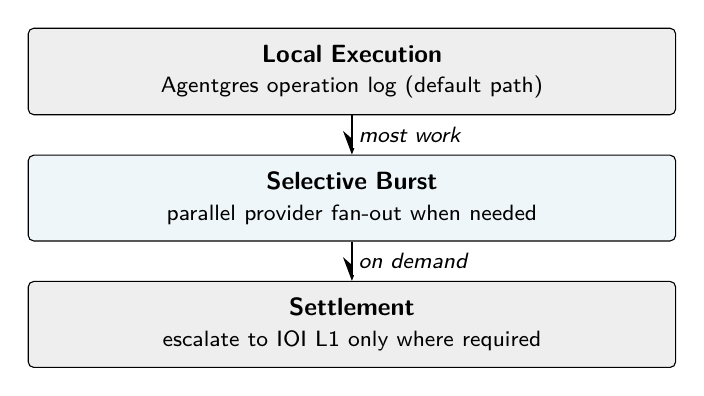
\begin{tikzpicture}[scale=1,transform shape,node distance=5mm and 10mm]
\node[ioiplain,text width=78mm] (loc) {\textbf{Local Execution}\\\footnotesize Agentgres operation log (default path)};
\node[ioibox,text width=78mm,below=of loc] (burst) {\textbf{Selective Burst}\\\footnotesize parallel provider fan-out when needed};
\draw[ioiflow] (loc) -- node[ioilabel,right]{most work} (burst);
\node[ioiplain,text width=78mm,below=of burst] (set) {\textbf{Settlement}\\\footnotesize escalate to IOI L1 only where required};
\draw[ioiflow] (burst) -- node[ioilabel,right]{on demand} (set);
\end{tikzpicture}
\end{center}


\hypertarget{execution-graph-runtime-view}{%
\subsubsection{4.8.1 Execution Graph (Runtime
View)}\label{execution-graph-runtime-view}}

At runtime, the DAG is compiled into canonical \textbf{ActionRequests}
and step-wise artifacts.

\textbf{Step-wise artifacts (normative): }Each node execution produces
an artifact bound to:

\begin{itemize}
\tightlist
\item
  \emph{canonical\_payload\_hash} of inputs/outputs,
\item
  \emph{policy\_hash},
\item
  \emph{model\_snapshot\_id} (when applicable),
\item
  and parent step references.
\end{itemize}

Graph and step addressing (normative):


\begin{center}
\needspace{6\baselineskip}
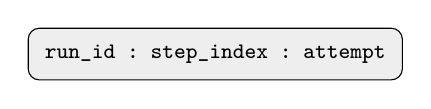
\begin{tikzpicture}[scale=1,transform shape,node distance=5mm and 10mm]

\node[draw,rounded corners,fill=ioibg,inner sep=6pt,font=\ttfamily\footnotesize]{run\_id : step\_index : attempt};
\end{tikzpicture}
\end{center}



\begin{center}
\needspace{6\baselineskip}
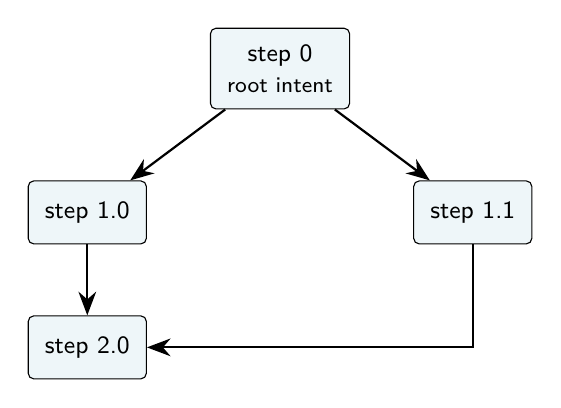
\begin{tikzpicture}[scale=1,transform shape,node distance=5mm and 10mm]

\node[ioibox] (s0){step 0\\\footnotesize root intent};
\node[ioibox,below left=9mm and 8mm of s0] (s1){step 1.0};
\node[ioibox,below right=9mm and 8mm of s0] (s2){step 1.1};
\node[ioibox,below=9mm of s1] (s3){step 2.0};
\draw[ioiflow](s0)--(s1);\draw[ioiflow](s0)--(s2);\draw[ioiflow](s1)--(s3);\draw[ioiflow](s2)|-(s3);
\end{tikzpicture}
\end{center}


\begin{longtable}[]{@{}
  >{\raggedright\arraybackslash}p{(\columnwidth - 0\tabcolsep) * \real{1.0000}}@{}}
\toprule\noalign{}
 \\
\midrule\noalign{}
\endhead
\bottomrule\noalign{}
\endlastfoot
Traceability:

Because each step commits to prior artifact IDs and utilizes hash-linked
receipt chains, final outputs carry a cryptographic chain-of-custody. A
calendar update can be traced back to the specific summary receipt(s),
policy, and required logs that authorized it. \\
\end{longtable}

\hypertarget{modular-dispute-resolution-privacy-preserving}{%
\subsubsection{4.8.2 Modular Dispute Resolution
(Privacy-Preserving)}\label{modular-dispute-resolution-privacy-preserving}}

Because verification is step-scoped, arbitration is precise:

\begin{itemize}
\tightlist
\item
  Disputes target \textbf{noncompliance} at a specific step, not ``the
  whole agent.''
\item
  Challenge packages can reference \emph{graph\_id} and \emph{step\_id}
  and reveal only minimal evidence for that step.
\item
  Arbitration evaluates only the contested step under its declared
  ruleset.
\end{itemize}

\textbf{Result: }Accountability without full disclosure.

\hypertarget{sparse-worker-categories-benchmarks-and-contribution-routing}{%
\subsection{4.9 Sparse Worker Categories, Benchmarks, and Contribution
Routing}\label{sparse-worker-categories-benchmarks-and-contribution-routing}}

The MoW worker economy requires a routing market that does not collapse
into one global leaderboard. IOI therefore supports \textbf{Sparse
Worker Categories}: narrow labor categories with explicit evaluation
profiles.

A Sparse Worker Category may declare required \emph{DomainOntology}
refs, \emph{CanonicalObjectModel} refs, \emph{WorkflowSchema} refs,
benchmark profile refs, \emph{EvaluationDataset} refs, privacy classes,
allowed training-data policies, and receipt obligations. Category claims
are comparable only when workers are evaluated against declared
ontology-bound inputs and rubrics.

\emph{aiagent.xyz} is the canonical product domain for Sparse Worker
Categories, Benchmark Profiles, worker manifests, trained worker
packages, installs, managed instances, ranking, and routing eligibility.
It may publish roots or commitments to IOI L1, but category operations,
benchmarks, installs, and marketplace projections are domain-level
Agentgres truth.

Examples:

\begin{enumerate}
\def\labelenumi{\arabic{enumi}.}
\tightlist
\item
  Rust security audit worker
\item
  legal intake worker
\item
  grant research worker
\item
  sales follow-up worker
\item
  React refactor worker
\item
  insurance claim review worker
\item
  construction quote worker
\item
  local SEO worker
\item
  government RFP worker
\end{enumerate}

Each Sparse Worker Category MAY define:

\begin{enumerate}
\def\labelenumi{\arabic{enumi}.}
\tightlist
\item
  task class
\item
  allowed input/output schemas
\item
  benchmark suite
\item
  evaluation rubric
\item
  runtime requirements
\item
  policy requirements
\item
  trust posture requirements
\item
  receipt obligations
\item
  submission fee or stake
\item
  routing eligibility criteria
\end{enumerate}

Submitting a worker to a category pays for benchmark execution and
leaderboard admission. A submitted worker does not automatically receive
routing. Routing eligibility is earned through benchmark performance,
receipt completeness, policy compatibility, price, and reputation.

Product usage and external compensation use separate ledgers:

Goal Space subscription $\rightarrow$ bounded Work Credits
$\rightarrow$ managed conductor/runtime/model/Worker/verifier usage
$\rightarrow$ itemized usage receipts

Network/Open funding $\rightarrow$ NetworkGoalBudget, bounty,
procurement cap, or ServiceOrder $\rightarrow$ independently admitted
contribution $\rightarrow$ verification and acceptance $\rightarrow$
separate fiat, stablecoin, IOI, or other approved settlement rail

Work Credits are non-transferable product budget units, not cash, Worker
payout, provider tokens, pooled seats, or the IOI protocol token.
ContributionReceipts and applicable verifier, acceptance, adjudication,
and settlement evidence determine external eligibility without turning
the subscription allowance into a vague pooled payout fund.

Reference payout structure:

worker\_payout = invocation\_fee + metered\_compute + success\_bonus +
quality\_delta\_bonus + royalty\_share - dispute\_or\_failure\_penalties

This structure supports direct invocation, outcome escrow, local
royalties, free/open Workers, and benchmark-funded category admission
while keeping product budget, contribution attribution, and payout
semantically separate.

\hypertarget{settlement-and-consensus}{%
\section{5. Settlement and Consensus}\label{settlement-and-consensus}}

\textbf{Implementation status: speculative target architecture.} IOI L1 is
not deployed in the current architecture baseline. This section describes
the bounded public-settlement role and candidate protocol profiles; it does
not claim a live chain, consensus deployment, validator set, escrow system,
or production token economy.

Settlement is \textbf{not runtime execution}, and local autonomous work
does not spam the public chain. Hypervisor nodes admit autonomous work and
local interop through the Daemon, Agentgres, and local receipt chains. IOI L1
is reserved for public or independent-trust boundaries involving registry,
rights, reputation, bonds, disputes, governance, economic settlement, or
selected roots. No chain or consensus step is required per OutcomeRoom,
GoalRun, frontier item, claim, attempt, finding, model invocation, receipt,
or Agentgres operation.

Non-Ownership Invariants:

-- IOI L1 does not own or store Hypervisor-node local settlement state.

-- IOI L1 does not own or record every governed autonomous-system-chain
transition.

-- IOI gas is not consumed for local settlement records or internal
module invocations.

-- A receipt or committed root retains its declared assurance stage; public
anchoring does not upgrade \emph{attested} or \emph{evidenced} work into
\emph{verified}, \emph{accepted}, \emph{adjudicated}, or \emph{settled}
work. The ordered assurance ladder is \emph{attested}, \emph{evidenced},
\emph{verified}, \emph{accepted}, \emph{adjudicated}, and \emph{settled}.

IOI L1 is designed as a bounded settlement, registry, dispute,
governance, and identity-anchor layer. It does not execute cognition; an
implemented settlement profile would receive selected consequences of
cognition executed elsewhere. Before a commitment can reach that boundary,
the underlying act must have crossed the Determinism Boundary and become a
transaction-shaped artifact: canonical, authorized, policy-bound,
receipt-backed, and challengeable.

Independent L1s and sovereign domains govern their own application state
independently. They may adopt IOI kernel / L0 releases by hash, policy,
and local governance decision, but IOI Mainnet does not manage their
ordinary state transitions. Such domains do not stream local execution
traces to the public L1; they maintain their own operational truth
locally within Agentgres or an equivalent domain substrate and would post
only sparse roots under explicit trigger events. A future IOI L1 may host
selected public registry, service-order commitment, dispute, bond,
reputation, rights, or governance contracts; Hypervisor execution and
provider placement do not depend on such a deployment.

This enables specialized autonomous-system economies (e.g., a medical
diagnosis consortium or an HFT domain) to coordinate as sovereign domains or run in
confidential/private execution environments while optionally anchoring
to Mainnet's bounded public primitives: settlement, arbitration,
registry, reputation, rights, and sparse verification commitments.

\hypertarget{the-role-of-ioi-l1-settlement-registry-and-disputes}{%
\subsection{5.1 The Role of IOI L1: Settlement, Registry, and
Disputes}\label{the-role-of-ioi-l1-settlement-registry-and-disputes}}

\textbf{The sparse L1 settlement boundary.} Under the edge-in topology,
\textbf{IOI L1} (and compatible execution chains) does not serve as an
active application runtime or general-purpose virtual machine. It is
optimized strictly as a secure, sparse ledger for public, economic, and
cross-domain commitments.

By default, all autonomous work, state transitions, model iterations,
and intermediate outputs are admitted locally inside \textbf{Agentgres} via
signed receipts, operation logs, and content-addressed artifact
references. This local execution layer is private by default and
decoupled from the public chain; disclosure depends on the selected
provider, cTEE posture, wallet.network authority, and declassification
policy. \textbf{The IOI L1 chain never reads, accesses, or processes raw
workspace contents, private memory, or unredacted workflows.}

Interaction with the public L1 ledger is entirely optional and strictly
\textbf{trigger-based}. A local domain kernel, Hypervisor Node, or
trusted local/client authority domain only escalates state commitments
upward to IOI L1 when a specific transactional boundary (such as
financial escrow, public licensing, service registry registration, or
SLA dispute arbitration) is crossed.

The trigger table below is a menu of optional public-settlement profiles,
not an automatic escalation policy. A marketplace listing, collaboration,
reputation observation, cross-domain exchange, or user archive remains
domain-local unless its governing parties intentionally select an
implemented public contract and the disclosure, authority, assurance, and
funding conditions for that contract are satisfied.

\textbf{L1 settlement triggers.}

\begin{longtable}[]{@{}
  >{\raggedright\arraybackslash}p{(\linewidth - 8\tabcolsep) * \real{0.2000}}
  >{\raggedright\arraybackslash}p{(\linewidth - 8\tabcolsep) * \real{0.2000}}
  >{\raggedright\arraybackslash}p{(\linewidth - 8\tabcolsep) * \real{0.2000}}
  >{\raggedright\arraybackslash}p{(\linewidth - 8\tabcolsep) * \real{0.2000}}
  >{\raggedright\arraybackslash}p{(\linewidth - 8\tabcolsep) * \real{0.2000}}@{}}
\toprule\noalign{}
& & & & \\
\midrule\noalign{}
\endhead
\bottomrule\noalign{}
\endlastfoot
Trigger Event & Description & L1 Action & Local / Domain Source & L1
Privacy Status \\
\textbf{Marketplace Listing} & Publishing a new worker capability for
discovery. & Registers the signed \emph{WorkerManifest} or package commitment
and license parameters on the public registry. & \emph{WorkerManifest} / aiagent.xyz
registry & \textbf{Public Metadata} (manifest hashes and capability
declarations only). \\
\textbf{ServiceOrder Commitment} & Establishing a formal delivery
agreement. & Records a public/economic commitment or locks escrow for a
\emph{ServiceOrder} bound to outcome terms, success schema, and
delivery/dispute rules. & \emph{ServicePackage} / sas.xyz proposal /
sas.xyz Agentgres state & \textbf{Public Metadata} (order commitment,
escrow, and settlement parameters only). \\
\textbf{Escrow / Payment} & Securing payment for an autonomous outcome.
& Locks or releases approved settlement assets under the selected escrow or
payment contract. & wallet.network payment authorization / settlement intent &
\textbf{Public Transaction} (addresses and token values only). \\
\textbf{SLA Dispute} & Contesting a failed outcome or delivery. &
Submits the contract-defined dispute and evidence commitments and locks any
required arbitration bond. & \emph{DeliveryBundle} / dispute package &
\textbf{Public Case Hash} (zero-knowledge / selective disclosure of the
failing step only). \\
\textbf{Rights / Licensing} & Minting and routing royalties for
intellectual property. & Records ownership transfers and routes runtime
execution royalty payments. & \emph{ServicePackageLicense} /
\emph{ContributionReceipt} & \textbf{Public Metadata} (license refs,
royalty splits, and package-right commitments only). \\
\textbf{Public Provider Commitment} & Anchoring a selected provider,
bond, reputation, or conformance claim. & Records the opted-in public
commitment; it does not publish provider credentials or become the
placement source. & \emph{HypervisorOSBootReceipt} / node manifest / assurance claim &
\textbf{Public Record} (declared metadata, commitments, and public keys only). \\
\textbf{Reputation Commit} & Anchoring a selected performance projection. &
Anchors a sparse Merkle root of task-performance evidence while preserving
each claim's assurance stage and challenge posture. &
Agentgres Quality Ledger / aiagent.xyz & \textbf{Public Root} (hash-only
representation). \\
\textbf{Cross-Domain Commitment} & Publishing a selected commitment from an
independent domain. & Registers the exact state or evidence commitment
accepted by the selected inter-domain contract. & \emph{AIIPEnvelope} /
state-root ref & \textbf{Public
Root} (hash-only representation). \\
\textbf{App-Chain Interop} & Exchanging value across distinct
application subnets. & Executes or records only the contract-approved value
transfer; it does not create a universal IOI bridge or import application
state. & \emph{LocalSettlementReceipt} &
\textbf{Public Transaction} (asset transfers and lock proofs only). \\
\textbf{User Public Commit} & Manual request for public timestamp, inclusion,
or ordering evidence. & Commits a snapshot of the current local state-root to
the public ledger. & \emph{AgentStateArchive} watermark & \textbf{Public
Root} (encrypted archive hash only). \\
\end{longtable}

An L1 commitment proves only the exact signature, inclusion, ordering,
contract transition, or proof-system statement covered by its profile. It
does not make an external-world assertion correct, establish contribution
causality, manufacture reviewer independence, or convert a provider-operated
fleet into multiple independent parties. Reputation, contribution, and
marketplace projections must preserve the assurance stage and the identities,
affiliations, verifier versions, disputes, and reversals that qualify the
underlying evidence.

IOI L1 is a proposed high-security ledger optimized for enforceability,
not raw interaction throughput or infrastructure discovery. It may anchor
selected public provider-registry, bond, reputation, rights, governance,
settlement, or dispute commitments. Hypervisor placement remains off-chain
and source-plural: candidates may come from direct adapters, connected or
customer inventories, managed capacity, DePIN or storage markets, and
optional \emph{decentralized.cloud}; Hypervisor admits the
PlacementDecision.

IOI L1 responsibilities are intentionally bounded:

\begin{enumerate}
\def\labelenumi{\arabic{enumi}.}
\tightlist
\item
  Public Coordination and Settlement Boundary
\end{enumerate}

\begin{itemize}
\item
  \begin{itemize}
  \tightlist
  \item
    \textbf{Balance Finality:} Maintains balances only for the settlement
    assets admitted by an implemented contract profile. Work Credits remain
    a product usage and budget abstraction unless an explicit settlement
    profile maps them to a settlement rail.
  \item
    \textbf{Escrow and commitment management:} Applies only the selected L1
    contract profile for public escrow, rights, bonds, disputes, payouts, or
    other economic finality. Routine provider billing and local Work Credit
    accounting do not become L1 channel state.
  \item
    \textbf{Fee Settlement:} Settles explicitly disclosed fees only where
    the selected contract requires public coordination or where paid
    optimized routing/procurement produced challengeable evidence. There is
    no generic cloud-session cut, local-work tax, receipt fee, authority fee,
    or Agentgres-write toll.
  \item
    \textbf{Bond Custody:} Custodies and enforces SLA collateral posted
    by Providers to collateralize declared uptime and honest-execution
    obligations under the relevant dispute rules.
  \end{itemize}
\end{itemize}

\begin{enumerate}
\def\labelenumi{\arabic{enumi}.}
\tightlist
\item
  Opt-In Dispute and Remedy Contracts
\end{enumerate}

\begin{itemize}
\item
  \begin{itemize}
  \tightlist
  \item
    \textbf{Dispute Intake:} Accepts only the dispute and evidence package
    declared by the selected contract profile and initiates that profile's
    verifier, appeal, and adjudication path.
  \item
    \textbf{Resolution Enforcement:} Executes a remedy only after the
    contract's authorized decision path reaches finality. There is no
    universal Arbitration Lane or automatic model judiciary.
  \end{itemize}
\end{itemize}

\begin{enumerate}
\def\labelenumi{\arabic{enumi}.}
\tightlist
\item
  Verification, Registry, and Rights Anchor
\end{enumerate}

\begin{itemize}
\item
  \begin{itemize}
  \tightlist
  \item
    \textbf{Optional Provider Registry Commitments:} May anchor opted-in
    public provider, conformance, bond, reputation, or dispute commitments.
    Direct adapters and candidate engines remain the placement sources; the
    public registry is never a mandatory provider gateway or credential
    store.
  \item
    \textbf{Identity Anchor:} May anchor public namespace, publisher,
    provider, domain, runtime, or manifest identity commitments.
    wallet.network and applicable domain owners retain identity operations,
    keys, authority grants, approvals, recovery, and revocation.
  \item
    \textbf{External Evidence Anchor:} May commit selected verifier-profile,
    evidence, or state roots required by a public contract. This is not a
    bridge and does not make IOI L1 the operational source of external state.
  \end{itemize}
\end{itemize}

\hypertarget{operational-invariant-optimistic-by-default}{%
\subsubsection{5.1.1 Operational Invariant: Optimistic by
Default}\label{operational-invariant-optimistic-by-default}}

The target IOI L1 posture is optimistic and sparse: local/domain runtimes
produce transaction-shaped acts, while a future public chain receives only
selected commitments under the active contract profile. Provider transport,
private workspace transfer, execution, and operational truth stay off-chain.
Public work is concentrated at declared boundaries:

\begin{itemize}
\tightlist
\item
  \textbf{Registry events:} Opted-in provider, capability, rights,
  reputation, conformance, or SLA-bond commitments.
\item
  \textbf{Settlement events:} ServiceOrder escrow, rights, payouts, bonds,
  and explicitly triggered public or cross-domain economic finality.
\item
  \textbf{Dispute events:} Contract-defined challenges, evidence verification,
  authorized decisions, appeals, and remedies.
\end{itemize}

The design objective is to keep effective interaction capacity at the edge
while making future IOI L1 load proportional to selected public/economic
events rather than cognitive steps; no quantitative throughput claim is made.

\hypertarget{modular-consensus-the-driver-philosophy}{%
\subsection{5.2 Settlement-Profile
Modularity}\label{modular-consensus-the-driver-philosophy}}

The IOI Runtime is \textbf{consensus-agnostic}. Runtime and domain
contracts should preserve common receipt and commitment semantics across
local authority, replicated domain, and future public-settlement profiles.
The current canonical architecture does not select or deploy a concrete IOI
L1 consensus engine, nor does it canonize a named consensus-driver ABI.

The Hypervisor Daemon enforces the daemon effect boundary, normalizes inputs,
and generates cryptographic receipts, but it does not dictate the
security model of a settlement domain. Illustrative profiles include:

\begin{itemize}
\tightlist
\item
  \textbf{Local authority mode:} A local Hypervisor Node or governed
  domain admits its own operations without public-network consensus.
\item
  \textbf{Replicated or federated domain mode:} A sovereign domain may
  select a BFT, Raft, multisignature, database-replication, or other
  agreement profile suited to its trust and availability model.
\item
  \textbf{Public settlement mode:} A future IOI L1 profile must declare
  exact consensus, finality, data-availability, challenge, verifier,
  governance, and adversary assumptions before it can carry public or
  irreversible economic commitments.
\end{itemize}

\hypertarget{driver-invariance-the-usb-c-rule}{%
\subsubsection{5.2.1 Settlement-Profile
Invariance}\label{driver-invariance-the-usb-c-rule}}

Changing the agreement or settlement profile must not silently change the
artifact meaning.

\begin{itemize}
\tightlist
\item
  \textbf{Schema Invariance:} A Receipt has the same canonical fields
  and hashing rules regardless of the settlement profile.
\item
  \textbf{Binding Invariance:} Canonicalization (RFC 8785),
  \emph{model\_snapshot\_id}, and \emph{policy\_hash} bindings remain
  identical.
\end{itemize}

What changes is the attestation class and available enforcement regime---not
the semantics of the artifacts. This supports Worker portability across the
fractal network: an artifact built and tested in a private enterprise domain
can be submitted to a compatible public settlement or adjudication profile
without redefining its canonical fields. Acceptance still depends on that
profile's authority, evidence, verifier, assurance, disclosure, and funding
requirements.

\hypertarget{aft-challenge-dominant-settlement-finality}{%
\subsection{5.3 Research Candidate: Challenge-Dominant Settlement
Finality}\label{aft-challenge-dominant-settlement-finality}}

This subsection records an \textbf{AFT research candidate} for a future
public settlement profile. It is not current architecture canon, not a
deployed IOI Mainnet engine, and not a quantitative security claim. Promotion
would require a canonical L1 owner update, formal specification, executable
conformance, independent review, and explicit synchrony, adversary,
data-availability, committee-selection, governance, and challenge-window
assumptions.

The candidate separates
throughput-critical publication from authority-critical verification.
Its goal is to make irreversible economic effects challenge-dominant and
fail-closed: if required observer, witness, or retrievability evidence
is missing or inconsistent, the slot aborts rather than settling unsafe
state. No claim is made here that this design exceeds classical BFT bounds
or is safe under a particular Byzantine threshold.

\textbf{Synchrony and challenge-epoch baseline.} The candidate assumes a
weak-synchrony model: after Global Stabilization Time (GST), public messages are delivered
within a bounded \(\Delta_{\mathrm{publish}}\), retrieval requests
complete or fail within \(\Delta_{\mathrm{retrieve}}\), and verification
finishes within \(\Delta_{\mathrm{verify}}\). A production deployment
sets an epoch duration \(T_{\mathrm{epoch}}\) and challenge duration
\(T_{\mathrm{challenge}}\) such that challenge publication, evidence
retrieval, recovery-capsule reconstruction, and verifier execution can
complete before the epoch closes. Any settlement commitment whose proof
depends on off-chain bytes MUST bind a retrievability window satisfying:

\[
T_{\mathrm{retrievable}} \geq
T_{\mathrm{challenge}} + \Delta_{\mathrm{publish}} +
\Delta_{\mathrm{retrieve}} + \Delta_{\mathrm{verify}}.
\]

If the respondent, provider, storage lane, or witness set fails to serve
the evidence required by the committed ArtifactRefs/PayloadRefs within
that epoch, the challenge is valid by absence. The challenged settlement
fails closed in favor of the challenger; no escrow release, slashing
defense, reputation update, or irreversible right transfer may depend on
bytes that were unavailable during the declared challenge epoch.

\hypertarget{the-two-tier-finality-model}{%
\subsubsection{5.3.1 The Two-Tier Finality
Model}\label{the-two-tier-finality-model}}

The research sketch uses a two-tier finality model that keeps block
transport on a fast finality lane, then upgrades selected slots to a stronger
irreversible-effect settlement state:

\begin{itemize}
\tightlist
\item
  \emph{BaseFinal}\textbf{ (Fast Finality Lane):} A validator majority Quorum
  Certificate (QC) plus a witness committee certificate. Used for rapid
  chain progression.
\item
  \emph{SealedFinal}\textbf{ (The Irreversible Path):} Upgrades
  \emph{BaseFinal} using a deterministic sealing plane. Irreversible
  effects (e.g., releasing a service outcome escrow) require a
  proof-carrying \emph{SealObject} that binds the observer/witness
  sealing surface.
\end{itemize}

Ambiguity or adversarial behavior during the sealing phase collapses
deterministically to \emph{Abort}, preventing the network from
heuristically retrying or partially settling unsafe state.

\hypertarget{canonical-challenge-v1-deterministic-observer-sealing}{%
\subsubsection{5.3.2 Canonical Challenge V1: Deterministic Observer
Sealing}\label{canonical-challenge-v1-deterministic-observer-sealing}}

To upgrade a block to \emph{SealedFinal} without requiring
\textgreater2/3 honest voting, the sketch considers \textbf{Deterministic
Observer Sealing}.

Observers are assigned deterministically via an epoch seed. Each
observer evaluates the block and publishes exactly one of two objects:

\begin{itemize}
\tightlist
\item
  A guardian-backed \emph{AsymptoteObserverTranscript} (\emph{Ok}).
\item
  An objective \emph{AsymptoteObserverChallenge} (e.g.,
  \emph{MissingTranscript}, \emph{TranscriptMismatch}).
\end{itemize}

The observer acceptance rule is strictly \textbf{challenge-dominant}:

\begin{itemize}
\tightlist
\item
  \emph{SealedFinal} is accepted if and only if the
  \emph{TranscriptSurface} covers every assignment and the
  \emph{ChallengeSurface} is empty under the declared challenge rules,
  emitting an
  \emph{AsymptoteObserverCanonicalClose}.
\item
  If \emph{any} valid challenge exists, the slot deterministically emits
  an \emph{AsymptoteObserverCanonicalAbort}.
\end{itemize}

Because canonical close and canonical abort are mutually exclusive, a
challenge-dominated slot cannot authorize irreversible release. Under
the declared data-availability, challenge-window, and publication
assumptions, any eligible observer able to publish an objective challenge
can prevent unsafe settlement and route the slot into the configured
remedy or slashing path.

\hypertarget{endogenous-retrievability-witness-coded-recovery-capsules}{%
\subsubsection{5.3.3 Endogenous Retrievability: Witness-Coded Recovery
Capsules}\label{endogenous-retrievability-witness-coded-recovery-capsules}}

To make the ordered set uniquely recoverable under declared
data-availability assumptions, the sketch considers an
\textbf{Endogenous Retrievability Plane} via nested witness committees.
Any quantitative withholding threshold is a parameter of the production
driver, committee-selection model, coding scheme, and challenge window,
not a universal guarantee of the abstract architecture.

\begin{itemize}
\tightlist
\item
  \textbf{Witness-Coded Recovery:} The protocol uses abstract coded
  recovery families (e.g., \emph{SystematicXorKOfKPlus1V1} or
  \emph{SystematicGf256KOfNV1}) to generate \emph{RecoveryCapsules}.
\item
  \textbf{Reconstruction:} Threshold-many public
  \emph{RecoveryShareMaterial} reveals can reconstruct the payload,
  outputting a compact \emph{RecoveredPublicationBundle}.
\item
  \textbf{Fail-Closed Impossibility:} If assigned witnesses fail to
  reveal their shares, the network accumulates
  \emph{MissingRecoveryShare} objects. Once the missing count exceeds
  the threshold required for recovery, the protocol materializes a
  deterministic \textbf{recovery-impossible canonical abort}.
\end{itemize}

This ensures that the protocol does not stall indefinitely waiting for
withheld data; it either recovers the payload or objectively aborts,
maintaining the challenge-dominant safety property declared in the
production specification.

The Witness-Coded Recovery Capsule is therefore part of the data
availability contract, not a replacement for it. A recovery capsule is
valid only when its reveal schedule, coding threshold, and retrieval
deadline fit inside the active challenge epoch. If recovery shares or
raw payload bytes are not served in time, the resulting
\emph{MissingRecoveryShare} or \emph{MissingEvidence} object is enough
to defeat the challenged settlement path.

\hypertarget{challenge-dominant-settlement-for-the-agentic-economy}{%
\subsubsection{5.3.4 Challenge-Dominant Settlement for the Agentic
Economy}\label{challenge-dominant-settlement-for-the-agentic-economy}}

Because the IOI kernel / L0 substrate is consensus-agnostic, agents
execute their logic off-chain, inside Hypervisor domains, or inside
independent sovereign domains. IOI L1 is the public settlement venue for
economic commitments, rights, disputes, reputation, and sparse roots
where authority-critical effects become public and economically
irreversible.

AFT's design intent is that authority-critical settlement is
challenge-dominant: under the declared synchrony, data-availability, and
observer-coverage assumptions, missing or inconsistent evidence aborts a
slot before unsafe state can settle. The exact adversary tolerance is a
function of those assumptions and the active challenge windows;
quantitative Byzantine thresholds are stated only in the production
Mainnet specification, not in this whitepaper.

The architectural goal is to remove reliance on dense validator quorums
for safety: settlement should fail closed when required evidence is
unavailable, rather than rely on majority honesty alone.

\hypertarget{the-settlement-core}{%
\subsection{5.4 Future Settlement Contract
Profiles}\label{the-settlement-core}}

Future IOI L1 settlement contracts are the public ingress/egress profiles for
selected registry, rights, reputation, bond, dispute, governance, and
economic commitments. They are not the execution runtime or a universal
adjudicator; each profile declares its inputs, evidence, verifier, authority,
finality, appeal, and remedy rules.

\hypertarget{settlement-pipeline}{%
\subsubsection{5.4.1 Settlement Pipeline}\label{settlement-pipeline}}

Any settlement artifact (Commitment, Bond Claim, Dispute) must pass the
pipeline:

\begin{enumerate}
\def\labelenumi{\arabic{enumi}.}
\tightlist
\item
  \textbf{Ingestion:} The selected settlement profile receives a declared
  \emph{SettlementEnvelope}, settlement intent, bond claim, rights commitment,
  or dispute package.
\item
  \textbf{Artifact Verification:} Validates the applicable canonical
  commitments, authority refs, signatures, receipt/evidence roots, contract
  profile, and funding or bond conditions without ingesting ordinary runtime
  history.
\item
  \textbf{Evidence Review (Optional):} If the settlement involves a
  disagreement regarding external outcomes, the selected verifier checks the
  attached EvidenceBundle under the contract's declared coverage and
  assumptions.
\item
  \textbf{Resolution \& Release:} Based on the authorized decision and
  covered evidence, the contract initiates the financial logic. The actual
  transfer of assets (releasing escrows, slashing bonds, or transferring
  package/license royalties) is explicitly held until the selected
  settlement profile reaches its required finality condition.
\end{enumerate}

\hypertarget{driver-based-interoperability}{%
\subsubsection{5.4.2 Driver-Based
Interoperability}\label{driver-based-interoperability}}

IOI enables agents to interact with any external system, blockchains,
cloud APIs, or legacy databases, through I/O Drivers.

\begin{itemize}
\tightlist
\item
  \textbf{No "Native" Chains:} The protocol treats Ethereum, Solana, and
  AWS equally: they are external systems accessed via tools.
\item
  \textbf{wallet.network capability strategy:} Interoperability is achieved
  through scoped authority and capability execution, not state bridging.
  wallet.network is mandatory when portable delegated authority, secrets,
  spend, declassification, or high-risk external effects are involved;
  local/domain governance may own ordinary local decisions. Agents request
  exact intents; the applicable authority path and daemon gate admit or deny
  them; and the tool/driver broadcasts only approved transactions.
\item
  \textbf{Atomic Swaps:} Cross-chain value transfer is handled via
  standard Hashed Timelock Contracts (HTLCs) or liquidity solver
  networks orchestrated by the agent, rather than a native IOI bridge
  protocol.
\end{itemize}

\hypertarget{domain-networks-sovereign-domains-and-l0-instantiated-execution-domains}{%
\subsection{5.5 Domain Networks, Sovereign Domains, and L0-Instantiated
Execution
Domains}\label{domain-networks-sovereign-domains-and-l0-instantiated-execution-domains}}

The \textbf{IOI kernel / L0 substrate} may instantiate domain networks,
sovereign execution domains, non-intelligent chains/state machines, and
intelligent blockchains. These domains can use their own consensus,
state, policy, receipts, and projection machinery. IOI L1 does not
become their application runtime; it can anchor their release roots,
registry commitments, settlement claims, governance approvals, and
dispute outcomes.

Sovereign domains, independent L1s, and intelligent blockchains are
formally instantiated through daemon/domain contracts that
\textbf{Hypervisor CLI/headless} and IOI protocol subcommands can
scaffold, submit, inspect, and verify. This is the developer-grade,
kernel-adjacent operator path for defining domain topology, policy
roots, manifests, receipts, and delegation models. The client does not
own the L0 substrate and does not bypass daemon or domain-kernel APIs;
it is not a standard Web2 SaaS dashboard, but it is still a
protocol-facing operator path for domain construction.

Because the network operates as an operating substrate rather than a
monolithic chain, a sovereign domain is an independent deployment that
uses IOI kernel/L0 primitives, domain contracts, or SDK releases where
they fit its trust model.

\hypertarget{the-independent-domain-thesis}{%
\subsubsection{5.5.1 The Independent Domain
Thesis}\label{the-independent-domain-thesis}}

Unlike traditional Web3 L2 rollups designed to offload execution from a
congested L1, IOI domains and independent L1s do not rely on IOI L1 for
execution, validation, or anchoring by default. They are
independent trust domains that may adopt the same kernel/L0 substrate,
schemas, receipts, and AIIP conventions.

\begin{enumerate}
\def\labelenumi{\arabic{enumi}.}
\tightlist
\item
  \textbf{Execution Separated from Coordination:} Cognitive work
  executes on user or provider hardware, while the sovereign domain tracks
  the canonical coordination state, object transitions, leases,
  receipts, and projection checkpoints required by that trust domain.
\item
  \textbf{Federated Consensus:} Domain deployments (e.g., a hospital
  consortium, a trading firm) compile the L0 Kernel and run validators
  on their own infrastructure using a declared replicated or federated
  agreement profile. They reach local agreement over domain state
  without publishing sensitive data or paying gas to public IOI L1.
\item
  \textbf{API-Native Interoperability Without Mandatory Enshrined
  Bridging:} Sovereign domains and independent L1s do not inherently need complex,
  protocol-enshrined bridges to communicate with the outside world. They
  expose standard gRPC or HTTP REST endpoints. Because they run the IOI
  SDK, a declared adapter may package selected API responses as canonical JSON
  with the applicable AIIP envelope, signature, and receipt refs. An external
  client can verify those exact signatures and commitments against the
  domain's declared public keys and profile off-chain; ordinary API responses
  do not become receipted or trusted automatically.
\end{enumerate}

\hypertarget{deployment-topologies}{%
\subsubsection{5.5.2 Deployment
Topologies}\label{deployment-topologies}}

Rather than a strict hierarchy, the IOI ecosystem supports parallel
deployment topologies tailored to different trust and coordination
requirements:

\begin{itemize}
\tightlist
\item
  \textbf{Future IOI Mainnet (Public Utility):} Uses a consensus and
  finality profile selected only after canonical specification and review.
  It may host selected public \emph{ai://} registry, service-order,
  rights, reputation, bond, governance, settlement, and dispute
  commitments without becoming the provider-discovery or execution layer.
\item
  \textbf{Sovereign Domains / Independent L1s (App-Specific):} Select a
  declared agreement profile suited to their trust model. Handles
  domain-specific coordination, internal app serving, and enterprise
  workspaces. They manage their own internal state and do not anchor to
  IOI Mainnet unless explicitly exporting trust or participating in
  cross-domain public settlement.
\end{itemize}

\hypertarget{cryptography-and-evidence}{%
\section{6. Cryptography and Evidence}\label{cryptography-and-evidence}}

This section specifies the cryptographic primitives the IOI architecture
requires. The protocol is designed for institutional risk models:
cryptography that remains durable under future cryptanalytic shifts, and
evidence interfaces that verify external state without trusting opaque
APIs or centralized bridges.

The protocol enforces two primary invariants:

\begin{enumerate}
\def\labelenumi{\arabic{enumi}.}
\item
  \textbf{Longevity: }artifacts and identities remain secure against
  future cryptanalytic shifts, including large-scale quantum
  adversaries.
\item
  \textbf{External Evidence Verification:} the kernel can verify claims
  about external state (e.g., Ethereum transactions, Solana proofs)
  under explicit driver-specific verification rules, without maintaining
  active light clients or trusting centralized bridges.
\end{enumerate}

\hypertarget{strict-hybrid-cryptography-classical-post-quantum}{%
\subsection{6.1 Strict Hybrid Cryptography (Classical +
Post-Quantum)}\label{strict-hybrid-cryptography-classical-post-quantum}}

Post-quantum algorithms are newer and may carry undiscovered design or
implementation risk. IOI therefore targets \textbf{hybrid classical and
post-quantum profiles} for long-lived identity, authority, policy,
transport, archive, and public-commitment use where the risk model requires
them. Exact suites are versioned wallet/transport/verifier profiles, not
timeless launch invariants in this whitepaper. The current architecture
canon does not select a genesis suite or claim a deployed post-quantum
network.

\begin{itemize}
\tightlist
\item
  \textbf{Root and recovery profile:} A versioned wallet profile may bind
  classical and post-quantum root material, factors, guardians, threshold
  shares, recovery posture, and legacy-asset compatibility. The derivation
  and mnemonic scheme must be specified and reviewed by the wallet owner
  before use.
\item
  \textbf{Transport profile:} A versioned application-layer hybrid KEM
  profile may combine approved classical and post-quantum mechanisms to
  reduce harvest-now/decrypt-later risk. Algorithm choice, parameter set,
  transcript binding, downgrade resistance, and rotation policy belong to
  the selected profile.
\item
  \textbf{Identity and policy profile:} Long-lived authority artifacts may
  require conjunctive classical and post-quantum signatures under a
  versioned profile. Verifiers must bind the exact algorithms, parameters,
  domain separation, expiry, and revocation posture rather than accepting a
  generic ``PQ secure'' label.
\item
  \textbf{Data-at-rest profile:} Wallet, memory-vault, archive, and
  context-projection and private-workspace-capsule encryption uses an approved
  authenticated-encryption profile
  with explicit key lifecycle, rotation, erasure, recovery, and algorithm
  agility.
\end{itemize}

\begin{longtable}[]{@{}>{\raggedright\arraybackslash}p{\linewidth}@{}}
\toprule\noalign{}
 \\
\midrule\noalign{}
\endhead
\bottomrule\noalign{}
\endlastfoot
\textbf{Target invariant:}\emph{\textbf{ }}Long-lived security claims
must name a versioned cryptographic profile, its assumptions, key lifecycle,
verifier support, and rotation path. No algorithm label by itself guarantees
decades of security. \\
\end{longtable}

\hypertarget{the-eei-external-evidence-interface}{%
\subsection{6.2 The EEI: External Evidence
Interface}\label{the-eei-external-evidence-interface}}

IOI is not a bridge. The L0/domain substrate and Hypervisor Daemon do not
need to maintain active light clients or sync external blockchain
headers. Instead, external-state claims use a passive evidence model:
participants submit structured evidence bundles and a declared verifier
evaluates the exact claim under a named rule, version, and assumption set.

To support a claim that an external event occurred (e.g., "This transaction
was confirmed on Ethereum" or "This bank API returned 200 OK"), participants
use the \textbf{External Evidence Interface (EEI)}.

EEI is what lets an IOI act remain transaction-shaped even when the
external consequence occurs outside IOI. The IOI receipt attests the declared
request, policy, authority decision or grant ref, actor, and runtime boundary
facts covered by its profile. The EEI bundle supplies provenance-bearing
support for the external-consequence claim. Verification, acceptance,
adjudication, and settlement remain separate assurance stages.

\hypertarget{evidence-bundles}{%
\subsubsection{6.2.1 Evidence Bundles}\label{evidence-bundles}}

The EEI defines a standard schema for wrapping external data so it can be
evaluated by the verifier or adjudication path named in the governing contract.
An Evidence Bundle consists of:

\begin{enumerate}
\def\labelenumi{\arabic{enumi}.}
\tightlist
\item
  \textbf{The Claim:} A canonical JSON object describing the event
  (e.g., \emph{\{ "chain": "eth", "tx\_hash": "0x...", "event":
  "Transfer", "amount": 100 \}}).
\item
  \textbf{The Proof: }Cryptographic material supporting the claim. This
  is driver-specific:
\item
  \textbf{For Blockchains:} An RPC receipt proof, a merkle inclusion
  proof, or a block header signed by a known oracle/notary.
\item
  \textbf{For Web APIs:} A TLSNotary proof or a signed attestation from
  a Multi-Party Computation (MPC) witness.
\item
  \textbf{The Binding:} A hash link to the specific \textbf{Agent Action
  Receipt }that triggered the external event.
\end{enumerate}

\textbf{Normative Invariant (Zero-Bloat Verification):} The firewall
evaluates chain-visible manifests and receipts that bind
\emph{request\_hash} to \emph{evidence\_hash}. Raw local bytes remain in
local memory/artifact storage behind Agentgres-governed refs; only the
canonical hash crosses to consensus.

\hypertarget{verification-via-drivers}{%
\subsubsection{6.2.2 Verification via
Drivers}\label{verification-via-drivers}}

The Kernel does not verify the Evidence Bundle natively. Instead,
verification is delegated to the \textbf{Driver }that generated the
action.

\begin{itemize}
\tightlist
\item
  \emph{Example:} If an agent uses the \emph{driver::eth\_wallet} to
  send funds, that driver includes the logic to parse and validate an
  Ethereum Receipt.
\item
  \textbf{Verification and adjudication role:} A declared verifier may load
  the relevant versioned Driver Plugin to validate the Evidence Bundle. A
  passing result means only that the named claim satisfied that verifier's
  rule and evidence coverage. The applicable counterparty may then accept it,
  a declared adjudicator may resolve a challenge, and a settlement profile may
  consume the accepted or adjudicated result.
\end{itemize}

\begin{longtable}[]{@{}
  >{\raggedright\arraybackslash}p{(\columnwidth - 0\tabcolsep) * \real{1.0000}}@{}}
\toprule\noalign{}
 \\
\midrule\noalign{}
\endhead
\bottomrule\noalign{}
\endlastfoot
Chain of Custody:

The authority and daemon boundary binds the declared intent, policy, grant,
and execution facts. The versioned driver or verifier interprets the declared
external-evidence format. Neither role expands its claim beyond the evidence
and threat model it actually covers. \\
\end{longtable}

\hypertarget{canonicalization-the-common-tongue}{%
\subsection{6.3 Canonicalization: The Common
Tongue}\label{canonicalization-the-common-tongue}}

To enable seamless movement of artifacts between Local, and Global
environments, IOI enforces strict data canonicalization.\\

\begin{longtable}[]{@{}
  >{\raggedright\arraybackslash}p{(\columnwidth - 0\tabcolsep) * \real{1.0000}}@{}}
\toprule\noalign{}
 \\
\midrule\noalign{}
\endhead
\bottomrule\noalign{}
\endlastfoot
Normative Standard (External):

\textbf{RFC 8785 (JSON Canonicalization Scheme, JCS)}, which builds on
I-JSON constraints and deterministic property sorting to produce a
hashable representation. ({[}RFC Editor{]}{[}2{]}) \\
\end{longtable}

\hypertarget{determinism-invariant}{%
\subsubsection{6.3.1 Determinism
Invariant}\label{determinism-invariant}}

Before hashing or signing, runtimes \textbf{MUST} canonicalize payloads:

\begin{itemize}
\tightlist
\item
  No whitespace variance
\item
  Deterministic key ordering (UTF-16 code unit order,
  locale-independent)
\item
  Reject \emph{NaN}/\emph{Infinity}
\item
  Economically meaningful quantities \textbf{MUST NOT} use JSON numbers;
  represent as fixed-point \textbf{strings} at the schema layer
\end{itemize}

\hypertarget{canonical_payload_hash}{%
\subsubsection{\texorpdfstring{6.3.2
\emph{canonical\_payload\_hash}}{6.3.2 canonical\_payload\_hash}}\label{canonical_payload_hash}}

Every IOI artifact is identified by a hash computed over canonical
bytes:


\begin{center}
\needspace{6\baselineskip}
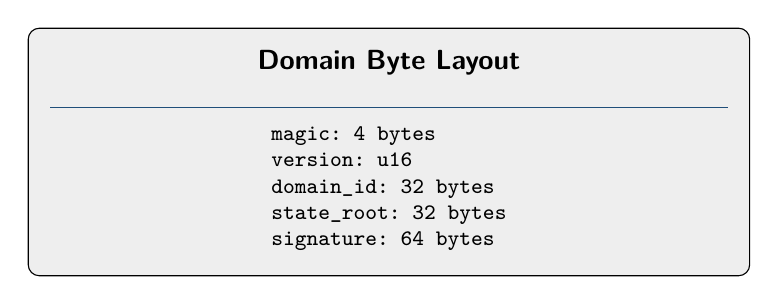
\begin{tikzpicture}[scale=1,transform shape,node distance=5mm and 10mm]
\node[draw,rounded corners,fill=ioibg,inner sep=8pt]{%
\begin{minipage}{86mm}
\centering{\sffamily\bfseries Domain Byte Layout}\par\vskip2pt
{\color{ioikw}\rule{\linewidth}{0.4pt}}\par\vskip4pt
{\ttfamily\footnotesize\begin{tabular}{@{}l@{}}
magic: 4 bytes\\
version: u16\\
domain\_id: 32 bytes\\
state\_root: 32 bytes\\
signature: 64 bytes
\end{tabular}}
\end{minipage}};
\end{tikzpicture}
\end{center}


\hypertarget{domain-separation}{%
\subsection{6.4 Domain Separation}\label{domain-separation}}

To prevent replay across contexts, IOI enforces strict domain
separation:


\begin{center}
\needspace{6\baselineskip}
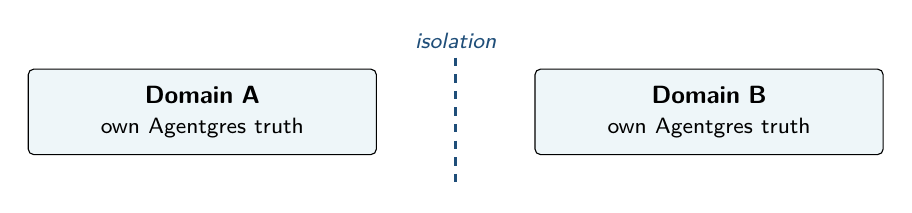
\begin{tikzpicture}[scale=1,transform shape,node distance=5mm and 10mm]
 % domain separation
\node[ioibox,text width=40mm] (a){\textbf{Domain A}\\\footnotesize own Agentgres truth};
\node[ioibox,right=20mm of a,text width=40mm] (b){\textbf{Domain B}\\\footnotesize own Agentgres truth};
\draw[ioikw,very thick,dashed] ($(a.east)!0.5!(b.west)+(0,0.9)$) -- ($(a.east)!0.5!(b.west)+(0,-0.9)$) node[ioilabel,pos=0]{isolation};
\end{tikzpicture}
\end{center}


Each cryptographic owner declares versioned domain-separation labels for its
artifact and signature families. Illustrative categories include:

\begin{itemize}
\tightlist
\item
  public block or commitment headers;
\item
  runtime and settlement receipts;
\item
  dispute and remedy decisions; and
\item
  manifests, packages, and releases.
\end{itemize}

Exact byte labels are not fixed by this synthesis; a verifier must reject an
unknown or mismatched profile rather than guess a domain.

\hypertarget{cryptographic-agility-verifier-registry}{%
\subsection{6.5 Cryptographic Agility (Verifier
Registry)}\label{cryptographic-agility-verifier-registry}}

Instead of treating algorithms as timeless constants, implementations use a
versioned \textbf{Verifier Registry} abstraction:

Algorithm\_ID → Verifier\_WASM\_Blob

\textbf{Upgrade path: }domains may add signature schemes or proof verifiers
through their declared governance and module-update path. A future IOI L1 may
anchor an on-chain registry, but no deployed registry or genesis suite is
claimed here.

\hypertarget{proof-carrying-private-execution-envelopes}{%
\subsection{6.6 Proof-Carrying Private Execution
Envelopes}\label{proof-carrying-private-execution-envelopes}}

\textbf{Private execution is substrate-neutral.} IOI does not require
Trusted Execution Environments as a root of authority. TEEs may be used
as one admissible execution substrate for confidentiality and
operational practicality, but they do not define validity. A private
execution claim advances only when its evidence satisfies the declared
receipt and verifier profile for its action class. Acceptance, adjudication,
and settlement are later contract states rather than implications of receipt
sufficiency. Where feasible,
IOI prefers proof-carrying computation --- including zero-knowledge
proofs, verifiable computation, FHE-backed private evaluation, MPC, or
hybrid constructions --- because these reduce reliance on hardware
attestation roots and align private execution with the protocol's
deterministic settlement model.

IOI treats private execution as a substrate-neutral evidence problem. A
private execution envelope may protect confidentiality, correctness, or
both:

\begin{enumerate}
\def\labelenumi{\arabic{enumi}.}
\tightlist
\item
  \textbf{Confidentiality:} The worker computes over sensitive inputs
  while minimizing disclosure. FHE and MPC can replace TEEs for bounded
  private evaluation where latency and cost permit.
\item
  \textbf{Correctness / Verifiability:} The worker proves that a
  committed computation was executed correctly. ZK-ML and verifiable
  computation can satisfy bounded inference, classifier, policy, or
  scoring claims without relying on a hardware vendor as the sole
  attestation root.
\item
  \textbf{Operational practicality:} TEEs remain admissible for running
  ordinary software with lower integration friction. In IOI they are
  treated as evidence adapters, not as protocol trust roots.
\end{enumerate}

Declared verifiers evaluate evidence sufficiency rather than treating
substrate identity as validity. The verifier registry therefore supports TEE quote verifiers,
ZK proof verifiers, MPC transcript validators, FHE parameter validators,
deterministic replay verifiers, and future proof systems. The canonical
verification question is not ``Did this run in a TEE?'' but ``Which exact
claim does this evidence establish under the required profile and threat
model?'' A settlement contract separately asks whether the claim reached its
required acceptance or adjudication state.

\textbf{Normative invariant:} A private execution substrate MUST NOT be
treated as a source of authority. Authority comes from the applicable
local/domain governance and wallet.network grant or approval path; hashes,
policy bindings, scopes, and receipts record and constrain that decision but
do not create it. The substrate contributes evidence only.

\hypertarget{the-privateexecutionenvelopereceipt}{%
\subsubsection{6.6.1 Private Execution Evidence and
CustodyProof}\label{the-privateexecutionenvelopereceipt}}

A \emph{CustodyProof}, TEE quote, ZK proof, MPC transcript, FHE
commitment, deterministic replay result, provider receipt, or hybrid bundle
is evidence, not an authority grant. Verifiers accept, reject, or mark a claim
inconclusive by checking the evidence profile required for the action and
privacy posture. No substrate label alone defines validity.

For Private Workspace backed by cTEE, the verifier-facing object is:

CustodyProof \{

\emph{proof\_id, workspace\_id,}

\emph{policy\_hash,}

\emph{sensitivity\_manifest\_hash, custody\_type\_derivation\_hash,}

\emph{mount\_graph\_hash, remote\_admissibility\_derivation\_hash,}

\emph{candidate\_lattice\_commitments,}

\emph{counterfactual\_lattice\_receipts, private\_operator\_receipts,}

\emph{declassification\_receipts, capability\_exit\_receipts,}

\emph{leakage\_receipts, state\_root\_before, state\_root\_after,}

\emph{verifier\_result: no\_plaintext\_custody | rejected | inconclusive}

\}

\hypertarget{identity-and-authority}{%
\section{7. Identity and Authority}\label{identity-and-authority}}

In the Internet of Intelligence, identity must bridge two worlds...
assets, reputation, and liability. \textbf{We are moving from Know Your
Customer (KYC) to Know Your Agent (KYA).}

KYA is the identity layer that lets Own become Act without becoming
ambient authority. It turns property rights into scoped, revocable,
receipt-backed execution authority.

\begin{itemize}
\tightlist
\item
  \textbf{KYC (Biological):} Validates \emph{who} you are (Passport,
  ID).
\item
  \textbf{KYA (Cryptographic):} Validates \emph{what} you are (Code
  hash), \emph{how} you behave (Policy envelope), and \emph{what} you
  are worth (Bonded Liability).
\end{itemize}

The IOI identity stack makes consequential work attributable inside its
applicable authority and truth domain; local-only work does not require a
public ledger identity.

IOI uses a \textbf{progressive identity model}. Users (and agents) are
not forced to manage seed phrases to begin; they start with device-local
authority and upgrade to network sovereignty only when they need to hold
funds or sign binding contracts.

\hypertarget{wallet.network-authority-and-access-point-profiles-legible-agency}{%
\subsection{7.1 wallet.network Authority and Access-Point Profiles (Legible
Agency)}\label{wallet.network-authority-and-access-point-profiles-legible-agency}}

\textbf{wallet.network} is the portable delegated-authority layer for
identity operations, secrets, capability leases, approvals, payments,
decryption, revocation, and audit lineage. Hypervisor and domain owners may
retain ordinary local governance, project policy, eligibility, and admission
decisions; wallet.network becomes mandatory when power must be portable,
revocable, secret-bearing, spend-bearing, declassification-bearing,
cross-domain, or executable by an autonomous worker. A
\textbf{guardian/access-point profile} may exist inside this
authority path as a device, browser, phone, enclave, threshold, or
daemon-adjacent policy/attestation role, but it is not a peer authority
system. The profile helps produce accountability attestations:
it can bind approval state, key-share use, policy hash, device posture,
or non-equivocation evidence into an append-only receipt chain.

This is what makes software legible to the economy: an agent can be
given a budget because its actions are auditable, bounded by policy,
and, when operating under enforceable modes, subject to slashing or
dispute enforcement.

\textbf{Implementation status.} Capability-lease authority, sealed
credentials, and approval gates are live in the daemon. Guardian surfaces,
key shards, and an MPC vault are planned; the profiles below are target
architecture where those facilities are not yet implemented.

\hypertarget{the-superset-identity-stack-master-vs.-ops}{%
\subsection{7.2 The Superset Identity Stack (Root Custody vs.
Execution)}\label{the-superset-identity-stack-master-vs.-ops}}

IOI explicitly separates the authority to act (Operational) from the
authority to own (Economic) while requiring the former to inherit
deterministic constraints from the latter. However, to prevent legacy
cryptographic vulnerabilities from compromising Web4 agency, IOI
defines a target \textbf{Cryptographic Superset Identity Model}. This model
avoids mandatory reliance on legacy EOAs by permitting a versioned
hybrid/PQ-aware
root for Web4 authority, while legacy-chain assets remain governed by
their native cryptographic assumptions and are risk-labeled accordingly.

The architecture defines a three-tier identity stack that progresses from
frictionless onboarding to institutional-grade security. Root generation,
recovery, classical/PQ composition, and legacy-asset compatibility are
versioned wallet profiles rather than one mandatory mnemonic construction.

Tier 1: Root Custody Profile

\begin{itemize}
\tightlist
\item
  \textbf{Role:} High-assurance custody of funds, a versioned identity
  anchor, and root policy authority for the user's wallet domain.
\item
  \textbf{Implementation profile:} A versioned wallet root and recovery
  profile may bind classical, post-quantum, threshold, guardian, and
  legacy-asset key material. It must declare derivation, export, recovery,
  rotation, revocation, and compatibility semantics explicitly.
\item
  \textbf{Function:} The Root Custody Profile serves as the highest-value
  "Source of Funds" and "Root of Policy." It is \textbf{never} directly
  connected to a high-frequency agentic workflow or dApp. It is secured
  by the user\textquotesingle s highest configured authentication
  threshold (e.g., 3FA/MPC). While users may optionally link a legacy
  Web3 hardware wallet (the "Link and Upgrade" bridge) as a liquidity
  source, the Root Custody Profile is the highest-assurance custody and
  recovery authority in the stack.
\end{itemize}

Tier 2: wallet.network Authority Core

\begin{itemize}
\tightlist
\item
  \textbf{Role:} Hot management of secrets, policies, session
  automation, and out-of-band approvals.
\item
  Implementation: \emph{wallet.network}, acting as the local authority,
  policy, secret-brokerage, approval, and revocation service.
\item
  \textbf{Cryptography:} Versioned classical/PQ signature, channel,
  vault-encryption, and recovery profiles selected by wallet.network policy
  and verified under their declared algorithms and parameters.
\item
  \textbf{Function:} The wallet.network Authority Core holds
  "Operational Authority." It
  evaluates agent requests against the user\textquotesingle s
  pre-approved Policy Envelope. Based on the user\textquotesingle s
  configured \textbf{Frictionless-to-Fortress} policy, it either
  auto-signs intents, executes capabilities internally via the
  brokered secret execution path, or triggers Step-Up MFA (e.g., FaceID
  or YubiKey) to mint time-bounded CapabilityLease objects,
  short-lived signer grants, and ApprovalTokens.
\end{itemize}

Tier 3: The Worker \& Agent Execution Account (Execution Layer)

\begin{itemize}
\tightlist
\item
  \textbf{Role:} Autonomous execution of tasks and on-chain
  interactions.
\item
  \textbf{Implementation:} CapabilityLease-bound short-lived signer
  grants used by the Agent Runtime, executing through an
  \textbf{Agent Execution Account}.
\item
  \textbf{The Smart Account Upgrade:} To ensure security survives a
  compromised runtime, the Agent Execution Account may be deployed as an
  ERC-4337 Smart Account.
\item
  \textbf{Function:} wallet.network Authority Core authorizes Tier 3
  CapabilityLease-bound signer grants as temporary module signers for
  the Smart Account.
  Workers operate autonomously within their granted scope. Crucially,
  \textbf{On-Chain Modules} (e.g., Spend Limits, Contract Allowlists)
  act as an on-chain enforcement backstop. Even if a local
  guardian/access-point profile is compromised or an agent goes rogue,
  smart-account policy can prevent the agent from draining funds beyond the module\textquotesingle s
  strict limits defined by the Root Custody Profile and active Policy
  Envelope.
\end{itemize}

Authority-Core Delegated Agent Autonomy:

In this architecture, agents do not generate raw signed transactions.
Instead, an agent generates a canonical \textbf{TxIntent}. The Tier 2
wallet.network Authority Core evaluates this intent against the Policy Envelope and the
user\textquotesingle s current security tolerance settings.

\begin{itemize}
\tightlist
\item
  \textbf{Low-Risk Intents} (e.g., read-only calls, allowlisted swaps)
  are processed with \textbf{Level 1 (Frictionless)} auth.
\item
  \textbf{High-Risk Intents} (e.g., modifying network allowlists,
  transfers exceeding caps) trigger an \textbf{Out-of-Band Step-Up},
  requiring the user to sign an \textbf{ApprovalToken} via a TEE-backed
  factor (FaceID) or a physical hardware key (YubiKey).
\end{itemize}

This model constrains the risk of the active execution environment away
from the user\textquotesingle s primary capital, enabling scalable
autonomy with bounded exposure, revocation, and receipt-backed
accountability rather than relying on the runtime to hold root custody.

The Link and Upgrade Bridge

The target Link and Upgrade profile does not require a legacy browser wallet
to become the Web4 authority root. A versioned wallet root/recovery profile may
combine classical, post-quantum, threshold, guardian, and legacy-asset factors
after its derivation and recovery design is specified and reviewed. A legacy
EOA may be linked through a signed proof such as SIWE for onboarding or
liquidity without upgrading the legacy chain's cryptographic assumptions. No
native PQ seed implementation is claimed by this whitepaper.

\hypertarget{wallet.network-the-authority-wallet-and-capability-layer}{%
\subsection{7.3 wallet.network: The Authority Wallet and Capability
Layer}\label{wallet.network-the-authority-wallet-and-capability-layer}}

To ensure that autonomous systems can act without usurping ownership,
Hypervisor routes portable delegated authority, secrets, spend,
declassification, and high-risk external effects through
\textbf{wallet.network} or an approved compatible authority client. Ordinary
local product governance may remain with its domain owner.

\textbf{wallet.network} is the canonical authority wallet and
capability layer of the machine economy. It controls custody policy,
key-use authority, policy grants, step-up challenges, secret leases,
payment scopes, decryption/viewing leases, and revocation epochs.

To prevent credential theft, raw secrets and private keys are never
stored on rented remote nodes, nor are they ever accessible to
autonomous workers. When a worker requires an external interaction
(e.g., executing a bank payment or modifying a cloud repository), it
cannot request raw credentials. Instead, the action must execute as a
\textbf{capability exit}: the Hypervisor Daemon intercepts the action
proposal and requests a short-lived, scoped cryptographic grant from
\emph{wallet.network}.

The protocol requires wallet.network or an approved compatible authority
client where work needs portable delegated authority, secrets, spend,
declassification, provider-trust acceptance, cross-domain reuse, or high-risk
external effects. Ordinary local governance may remain in Hypervisor or its
domain owner. wallet.network is the canonical portable identity-operation,
secret, authority-scope, approval, payment, and revocation layer for autonomous
software.

Architecturally, it functions as a \textbf{Cryptographic Superset}. A
versioned wallet profile may bind legacy-asset keys, native Web4 authority,
classical/PQ mechanisms, guardians, and threshold material without treating
one root algorithm as timeless protocol canon. It scales assurance through
configurable factor, guardian, quorum, and signature thresholds, allowing the
user or organization to define the balance between friction and high-assurance
control.

Core Capabilities:

\begin{itemize}
\tightlist
\item
  \textbf{Brokered Secret Execution:} Securely governs Web2 secrets (AWS,
  Stripe, OpenAI, broker APIs, cloud credentials, and similar external
  capabilities). It enforces a strict security invariant:
  \textbf{The agent requests effects, not keys.} The wallet.network
  authority path or configured secret provider never delivers durable raw
  credentials to the agent; it executes or authorizes the capability exit
  under a scoped lease and returns only policy-approved results.
\item
  \textbf{Frictionless-to-Fortress Auth:} Targets progressive security from
  low-risk identity-provider/passkey onboarding through device-backed and
  institutional threshold profiles; guardian and MPC-vault facilities remain
  planned.
\item
  \textbf{Zero-Trust Extensibility:} Provides a programmatic SDK and a
  sandboxed WASM marketplace for third-party developers to integrate
  custom API connectors securely.
\item
  \textbf{Unified Authority Audit:} Receipted visibility over mediated grant,
  denial, approval, credential-use, revocation, and applicable spend events.
  It does not create total observability over opaque models, providers, or
  unmediated external systems.
\end{itemize}

\textbf{Wallet action grammar.} wallet.network is not merely a
cryptographic keychain. It is the authority wallet for autonomous
finance and delegated capability use. Every meaningful action follows a
common grammar:

\begin{center}
\texttt{Intent -> Simulation -> Risk labels -> Policy check -> Approval or denial -> Execution -> Receipt}
\end{center}

This grammar applies to sends, receives, exchanges, trades, approvals,
delegations, revocations, protection actions, secret brokerage,
declassification, provider payments, and agent actions. Low-risk actions
may run inside a preapproved session envelope; high-risk actions require
one-shot or step-up approval bound to the exact request hash, policy
hash, grant or lease, revocation epoch, risk labels, and receipt
obligations.

The authority pipeline is reusable infrastructure; the full Wallet
console is only one presentation of it. Consumer apps may use compact
Lite Approval Cards, ordinary Wallet actions may use Standard Wallet
Review, and treasury, trading, Hypervisor, or developer workflows may
use an Advanced Authority Console with raw receipts, route candidates,
policy JSON, traces, and adapter evidence. The underlying contract is
the same: intent, simulation, risk and eligibility labels, policy
explanation, approval mode, execution handoff, typed receipt, and
revocation path.

\textbf{Wallet authority objects.} The reusable pipeline is
\textbf{WalletAuthorityCore}: the policy and review engine behind the
Wallet app, embedded dapp approvals, agents, Hypervisor prompts,
CLI/headless prompts, and advanced consoles. A
\textbf{WalletPresentationProfile} changes only presentation, never
policy or receipt semantics. Canonical presentation profiles include
\emph{lite\_approval\_card}, \emph{standard\_wallet\_review},
\emph{advanced\_authority\_console}, \emph{cli\_prompt}, and
\emph{mobile\_approval\_sheet}. An \textbf{ApprovalMode} is the
policy-derived posture for execution: \emph{one\_shot\_review},
\emph{session\_envelope}, \emph{batch\_review},
\emph{silent\_within\_policy}, \emph{after\_the\_fact\_receipt},
\emph{step\_up\_review}, or \emph{denied}. A
\textbf{RiskCoverageState} is attached to risk and eligibility labels:
\emph{Assessed}, \emph{Unknown}, \emph{Unassessed}, \emph{Stale},
\emph{Partially Covered}, or \emph{Conflicting Sources}. Apps may
request a presentation profile or approval mode, but wallet.network
derives the allowed mode from policy, risk, eligibility, account
posture, and active session state.

\textbf{Exchange and trade authority.} Exchange and trade are
first-class wallet actions, but route and venue sources are not trust
roots. \emph{decentralized.exchange} is a preferred first-party
route-intelligence engine for asset conversion; direct pools, routers,
solvers, aggregators, and user-specified routes may also propose
candidate \textbf{RouteCandidate} objects.
\emph{decentralized.trade} is a preferred first-party
venue/market/exposure-intelligence engine for spot orders, perps,
positions, prediction markets, and event contracts. These engines
produce candidates, metadata, risk evidence, simulations, and intent
templates. wallet.network evaluates policy, discloses risk, obtains
approval, signs or denies, emits typed receipts, and can revoke or
protect assets. Pools, venues, and chains perform execution; Agentgres
records receipt and evidence state.

Product packaging follows the same boundary. Wallet is the cockpit.
\emph{decentralized.exchange} and \emph{decentralized.trade} are
non-custodial API/RPC/SDK route-intelligence services consumed by
Wallet, Hypervisor, agents, and third-party clients. They may expose
docs, explorers, adapter registries, paper venues, or lightweight
standalone views, but the canonical Wallet user does not need to leave
wallet.network to review, approve, deny, execute, monitor, or receipt an
exchange or trade action.

Every route, venue, market, position, or prediction candidate must carry
\textbf{CandidateEvidence}: candidate id, source, adapter id, observed
timestamp, expiry, coverage state, evidence refs, risk labels,
eligibility labels, and explicit claims. A candidate without evidence is
not approval-eligible. Unknown, unassessed, stale, expired, or
conflicting-source candidate evidence cannot execute silently; it must
refresh, step up, enter paper mode, or be denied by wallet.network
policy.

The semantic wallet objects are \textbf{ExchangeIntent},
\textbf{TradeIntent}, and \textbf{PredictionIntent}. An ExchangeIntent
binds route, calldata commitments, slippage, simulation, policy, grants
or leases, revocation epoch, economics, risk labels, and exact
\textbf{TxIntent} records before a swap can be approved or signed. A
TradeIntent binds venue, market, side, collateral, leverage, margin
mode, order type, liquidation and funding assumptions, max-loss policy,
simulation, grants or leases, revocation epoch, risk labels, and exact
venue/order/TxIntent records. A PredictionIntent binds venue, market
question, outcome, side, price limit, shares, max loss, max payout,
resolution source, market rules, liquidity snapshot, grants or leases,
revocation epoch, and risk labels. Long-lived trading state is recorded
through typed receipts such as \textbf{PositionReceipt} and
\textbf{PredictionReceipt}; position risk and event-resolution risk must
not be hidden behind generic swap history.

\textbf{Asset exposure and protection.} Wallet must make risk
actionable, not merely descriptive. An \textbf{AssetExposureRecord}
summarizes each asset or account's cryptographic regime, public-key
exposure, bridge dependencies, admin-key dependencies, oracle
dependencies, approval exposure, agent-access exposure, policy
protection level, risk labels, and recommended
\textbf{ProtectionAction} refs. Protection actions include revoking or
reducing approvals, moving assets to fresher or stronger-policy
accounts, isolating agent execution funds from long-term custody,
requiring step-up for bridge or public-key exposure, pausing agent grant
access, or requiring org quorum for higher-risk routes. Each protection
action follows the same authority grammar and emits a
\textbf{ProtectionReceipt}.

\textbf{Approval inbox and typed receipts.} wallet.network exposes a
unified approval inbox made of \textbf{ApprovalInboxItem} records for
step-up requests, policy-widening requests, exchange exceptions, trade
exceptions, margin/leverage/perps requests, bridge-use requests,
unknown-contract requests, unlimited-approval requests, agent
delegations, secret-release requests, declassification requests,
high-value transfers, and org quorum requests. Every item must show
initiator, requested action, authority risk class, affected assets or
secrets, budget, destination, policy diff, simulation result, expiry,
and deny/edit/approve paths. The output is not one flat log: wallet
actions produce typed receipts such as \textbf{ExchangeReceipt},
\textbf{TradeIntentReceipt}, \textbf{PositionReceipt},
\textbf{PredictionIntentReceipt}, \textbf{PredictionReceipt},
\textbf{RiskEventReceipt}, and \textbf{ProtectionReceipt}, all under a
common wallet receipt envelope.

\textbf{Economic disclosure.} Exchange receipts must bind expected
output, minimum output, slippage tolerance, pool/protocol/wallet fees,
gas estimate, price impact, route source, quote source, execution venue,
bridge dependency, solver/RFQ dependency, and MEV/protection mode where
applicable. Advanced trade receipts must bind collateral, notional
exposure, leverage, margin mode, funding/borrow assumptions,
liquidation estimate, venue fees, oracle or mark-price source, max-loss
policy, stop-loss/take-profit posture, and eligibility restrictions.

The IOI monorepo owns the wallet protocol packages that make this
contract portable. \textbf{@ioi/wallet-protocol} exports wallet protocol
objects, method metadata, JSON Schema, OpenAPI, receipt fixtures, and
canonical examples tied to Rust wallet types and wallet service tests.
\textbf{@ioi/wallet-sdk} is a typed client/helper package over
\textbf{@ioi/wallet-protocol} for authority reviews, capability leases, receipts,
exchange, trade, and protocol method calls. Product repositories such as
wallet.network consume these packages; they do not author canonical
scopes, grants, leases, approval modes, receipts, CandidateEvidence,
ExchangeIntent, TradeIntent, PredictionIntent, CapabilityLease, or
authority semantics.

\textbf{Agent capabilities and leased credentials.} Agents do not hold
balances or secrets directly. They receive scoped capabilities such as
\emph{scope:gmail.send}, \emph{scope:broker.place\_order}, or
\emph{scope:cloud.deploy} under time-bounded \textbf{CapabilityLease}
objects,
caps, and step-up rules. Viewing/decryption rights are distinct from
use rights. Every grant, lease, use, denial, expiry, and revocation generates a
wallet.network receipt and, where operationally meaningful, an
Agentgres-linked receipt.

\textbf{Access points, guardians, and declassification.} Access points
(such as web portals, Discord bots, mobile apps, and SMS gateways) are
strictly delivery and monitoring interfaces; \textbf{they are not
authority roots}.

An SMS notification cannot authorize a transaction or decrypt a
workspace. If a high-risk action triggers a \textbf{StepUpChallenge},
the notification channel may only deliver an escalation link. The actual
authorization must occur by looping back to a verified, high-assurance
client --- such as an authenticated \textbf{phone/local guardian profile}, a
\textbf{Local Hypervisor App}, or an \textbf{Enterprise Key Service}.

For highly sensitive outputs leaving the private workspace, the client
acts as the default private view and declassification point. Any export
of protected state across the boundary must generate a
\textbf{DeclassificationReceipt}, validating that the data has passed
unredaction filters and was signed off by an authorized
\emph{wallet.network} key.

\textbf{Access assurance hierarchy.}

\begin{longtable}[]{@{}
  >{\raggedright\arraybackslash}p{(\linewidth - 8\tabcolsep) * \real{0.2000}}
  >{\raggedright\arraybackslash}p{(\linewidth - 8\tabcolsep) * \real{0.2000}}
  >{\raggedright\arraybackslash}p{(\linewidth - 8\tabcolsep) * \real{0.2000}}
  >{\raggedright\arraybackslash}p{(\linewidth - 8\tabcolsep) * \real{0.2000}}
  >{\raggedright\arraybackslash}p{(\linewidth - 8\tabcolsep) * \real{0.2000}}@{}}
\toprule\noalign{}
& & & & \\
\midrule\noalign{}
\endhead
\bottomrule\noalign{}
\endlastfoot
Access Point & Assurance Level & Custody \& Signer Status & Decryption
Capacity & Primary Threat Vulnerability \\
\textbf{SMS / Chat Bot} & \textbf{Low Assurance} & None. Cannot sign,
authorize, or hold keys. & None. Cannot decrypt any data. &
SIM-swapping, API gateway capture, and man-in-the-middle
interception. \\
\textbf{Browser Web Interface} & \textbf{Medium Assurance} &
Session-gated. Can hold transient keys in memory. & Restricted to local,
sandboxed session storage. & Cross-Site Scripting (XSS), malicious
extensions, browser-jacking. \\
\textbf{Local App / CLI/headless / optional TUI} & \textbf{High
Assurance} & Device-bound. Direct access to local OS sandboxing. & Can
decrypt local workspace databases. & Local system malware and physical
host capture. \\
\textbf{Phone / local guardian profile} & \textbf{High Assurance} & Hardware-enforced
(biometric secure enclaves). & Can decrypt restricted local archives. &
Physical device theft (gated by biometric checks). \\
\textbf{Enterprise Key Service} & \textbf{High Assurance} &
Institutional (MPC, multisig, HSM-gated). & Highly restricted,
role-based decryption. & Compromise of enterprise administrative
credentials. \\
\textbf{wallet.network} & \textbf{Root Authority} & Root custody policy,
key-use authority, policies, and grants. & Generates and manages
decryption/viewing leases. & Root credential, recovery, or policy
compromise. \\
\end{longtable}

\hypertarget{the-credential-enclave-capability-execution-secret-isolation}{%
\subsubsection{7.3.1 Brokered Secret Execution (Capability Execution \&
Secret
Isolation)}\label{the-credential-enclave-capability-execution-secret-isolation}}

Standard agents often require API keys in environment variables,
creating massive attack surfaces. The IOI architecture fundamentally
rejects this model. To achieve secure automation, \emph{wallet.network}
manages credentials exclusively through \textbf{Capability Execution}:

\begin{enumerate}
\def\labelenumi{\arabic{enumi}.}
\tightlist
\item
  \textbf{Storage (Data at Rest):} Keys are sealed under the selected
  versioned vault-encryption and key-derivation profile (which may use an
  approved construction such as XChaCha20-Poly1305 with an appropriate KDF).
  The profile keeps durable raw key material inaccessible to agent sandboxes.
\item
  \textbf{Request (The Intercept):} When an agent attempts a tool call
  (e.g., \emph{tools/call:stripe}), the Hypervisor Daemon sends an
  \emph{AuthorityScopeRequestEnvelope} directed at
  \emph{wallet.network}.
\item
  \textbf{Capability Execution:} The wallet.network Authority Core evaluates the request against
  the active Policy Envelope. If authorized (and MFA is satisfied), the
  Authority Core executes the capability internally- making the external API call
  or signing the transaction itself.
\item
  \textbf{Return (Sanitized Delivery):} \emph{wallet.network} returns
  only the sanitized result (e.g., the API response) to the agent
  daemon. \textbf{The secret never leaves
  }\emph{\textbf{wallet.network}}\textbf{'s authority custody path and
  never enters the agent's runtime space.}
\end{enumerate}

\hypertarget{the-multi-factor-identity-model-frictionless-to-fortress}{%
\subsubsection{7.3.2 The Multi-Factor Identity Model
(Frictionless-to-Fortress)}\label{the-multi-factor-identity-model-frictionless-to-fortress}}

The target wallet profile may use threshold cryptography, guardians,
hardware-backed factors, or an MPC vault to support progressive security.
Those key-shard and MPC-vault facilities are planned, not current baseline
claims:

\begin{itemize}
\tightlist
\item
  \textbf{Level 1 (Frictionless 1FA):} An identity-provider or passkey
  onboarding factor under a declared low-risk policy; it does not by itself
  mint broad autonomous authority.
\item
  \textbf{Level 2 (Trusted Device 2FA):} Mobile biometric enclaves and
  WebAuthn authenticators can provide a hardware-backed
  local-user-presence signal under the device vendor's security model.
  IOI treats this as a step-up authentication factor, not as a proof of
  legal identity or an infallible proof of physical presence. Mobile 2FA
  and SMS channels are classified as notification or step-up transport
  conduits; they cannot bypass the core cryptographic signature
  requirements of \emph{wallet.network}.
\item
  \textbf{Level 3 (High-Assurance 3FA+):} A planned configurable threshold
  or MPC profile using hardware keys, enrolled guardians, HSMs, or enterprise
  authority with explicit approval thresholds for high-stakes capital
  movement or policy widening.
\item
  \textbf{Sovereign Backup:} Users may use an approved portable recovery
  profile to exit one wallet.network interface while retaining authority
  over compatible assets, grants, and worker identities. The export must
  declare exactly which key families, factors, guardians, and domains are
  recoverable.
\end{itemize}

\hypertarget{session-keys-the-burner-wallet-pattern}{%
\subsubsection{7.3.3 Capability Leases and Short-Lived Signers
}\label{session-keys-the-burner-wallet-pattern}}

To operationalize the hierarchy, IOI implements capability delegation
via \textbf{CapabilityLease}-bound short-lived signer grants issued to
Tier 3 Workers. These are constrained by an explicit Policy Envelope
(specific capabilities + spend limits + target whitelists).

\begin{itemize}
\tightlist
\item
  \textbf{Expiry:} Leases and signer grants are strictly time- or
  block-bounded.
\item
  \textbf{Revocation:} Session authority can be revoked by
  wallet.network Authority Core at any time by advancing the
  \emph{revocation\_epoch},
  instantly invalidating the agent\textquotesingle s ability to act or
  spend.
\end{itemize}

\hypertarget{delegated-coordinator-profile-delegated-authority}{%
\subsubsection{7.3.4 Delegated Coordinator Profile (Delegated
Authority)}\label{delegated-coordinator-profile-delegated-authority}}

For complex multi-worker systems, the user may delegate coordination to a constrained
coordinator profile. Unlike a standard Worker, a coordinator may request
subordinate CapabilityLease grants for its subordinates, but only
through monotonic narrowing, wallet.network authority, and daemon
receipts.

\begin{itemize}
\tightlist
\item
  \textbf{Delegation Certificate:} To hire a worker, wallet.network
  Authority Core signs a certificate binding the new Worker\textquotesingle s
  ephemeral key or signer grant to a \textbf{monotonic narrowing} of the
  parent grant's budget and policy.
\item
  \textbf{Cascading Revocation:} wallet.network retains the root
  revocation path for active grants. Revoking the parent grant advances the relevant
  \emph{revocation\_epoch} and triggers cascading termination of all
  downstream leases, signer grants, and associated payment channels.
\end{itemize}

\hypertarget{zero-trust-extensibility-framework}{%
\subsubsection{7.3.5 Zero-Trust Extensibility
Framework}\label{zero-trust-extensibility-framework}}

wallet.network supports programmatic extensibility (see Section
7.3 for product surface details):

\begin{itemize}
\tightlist
\item
  \textbf{Permissionless Domain Integration:} Any third-party platform
  can integrate the open \textbf{@ioi/wallet-sdk} to request
  wallet.network authority reviews, CapabilityLeases, and receipts. The
  wallet.network authority path cryptographically verifies the origin
  and requires policy-compatible consent before issuing bounded session
  authority.
\item
  \textbf{Sandboxed Connector Marketplace:} Developers can build and
  publish new API connectors (e.g., custom CRM or niche banking APIs).
  These run inside a \textbf{hermetic WASM sandbox (WASI)} injected only
  with the specific secret required, physically preventing third-party
  logic from exfiltrating other wallet.network credential material.
\end{itemize}

\hypertarget{portable-app-sessions-agentgres-authority}{%
\subsection{7.4 Portable App Sessions and Authority
State}\label{portable-app-sessions-agentgres-authority}}

Centralized session state (cookies, JWTs against a single database)
breaks in a multi-plane architecture where users fail over between
provider environments.

IOI replaces centralized session state with \textbf{Stateless Portable
Capability Tokens}.

Rather than a node looking up a session in a local database, the client
holds a scoped \emph{HypervisorSessionAccessLease} and derived
\emph{SessionAccessToken} that dictate what canonical state it
can read, what projections it can subscribe to, and what mutations it
can request.

\textbf{Authority-bound restore.} Portable sessions restore through
authority-bound import. A sealed archive may contain task state, run
checkpoints, traces, artifact refs, patch branches, projection
checkpoints, and replay metadata. It should not silently mutate live
truth. The applicable authority provider validates restore power; daemon and
Agentgres admission validate the grant/lease refs, hash, policy, schema,
state root, object heads, and restore evidence before rehydration.

\hypertarget{the-stateless-authentication-flow}{%
\subsubsection{7.4.1 The Stateless Authentication
Flow}\label{the-stateless-authentication-flow}}

Portable session tokens carry an explicit cryptographic envelope
containing:

\begin{itemize}
\tightlist
\item
  \emph{session\_id} or \emph{lease\_id}
\item
  \emph{subject\_id} (The User/Principal) and \emph{issuer\_id} (the
  wallet.network Authority Core)
\item
  \emph{policy\_hash} (The overarching ruleset)
\item
  \emph{primitive\_capabilities}, \emph{authority\_scopes}, and
  \emph{projection\_scope} (what execution classes, delegated power, and
  Agentgres views are available)
\item
  \emph{expires\_at} and \emph{revocation\_epoch}
\end{itemize}

Because these tokens are self-contained and signed by the
user\textquotesingle s \emph{wallet.network} Authority Core, validation
does not require the original application database. It still must check
current expiry, revocation, audience, policy, and authority state. If the
active environment serving an \textbf{Agentgres} projection goes down,
the client seamlessly reconnects to a new healthy environment, presents
the same portable token, and
resumes its subscription stream. The new node validates the signature,
expiry, and capability scope against the canonical state without needing
a shared backend database.

\hypertarget{the-auth-split-portable-vs.-pinned-authority}{%
\subsubsection{7.4.2 The Auth Split: Portable vs. Pinned
Authority}\label{the-auth-split-portable-vs.-pinned-authority}}

To balance seamless application failover with strict security for
high-stakes actions, the KYA framework enforces a strict bifurcation in
how tokens are audience-bound:

\begin{enumerate}
\def\labelenumi{\arabic{enumi}.}
\tightlist
\item
  Portable Session/Lease Tokens (For App State):
\end{enumerate}

\begin{itemize}
\item
  \begin{itemize}
  \tightlist
  \item
    \emph{Usage:} Reading \textbf{Agentgres} projections, maintaining
    resumable subscriptions, and requesting routine workflow mutations.
  \item
    \emph{Audience Binding:} Bound to the \textbf{logical application
    instance} or runtime identity, \emph{not} a specific physical node.
    This ensures cross-node failover for normal app continuity.
  \end{itemize}
\end{itemize}

\begin{enumerate}
\def\labelenumi{\arabic{enumi}.}
\tightlist
\item
  One-Shot Approval Tokens (For High-Risk Execution):
\end{enumerate}

\begin{itemize}
\item
  \begin{itemize}
  \tightlist
  \item
    \emph{Usage:} Sensitive capability execution (e.g., spending funds,
    signing mainnet transactions, modifying core firewall policies).
  \item
    \emph{Audience Binding:} Tightly pinned to a specific physical
    executor or authority-profile ID via \emph{nonce}, \emph{counter},
    \emph{revocation\_epoch}, and strict \emph{audience} fields. These
    cannot be ported to another node; they are exact, single-use
    cryptographic authorizations.
  \end{itemize}
\end{itemize}

This model separates high-risk authority from the active execution
environment. It allows user interfaces to remain fast, distributed, and
highly available via \textbf{Agentgres}, while requiring irreversible
sovereign actions to remain explicitly gated, audience-bound, and
receipt-backed.

\hypertarget{authority-scope-request-flow}{%
\subsection{7.5 Authority Scope Request
Flow}\label{authority-scope-request-flow}}

\textbf{The core architectural doctrine of IOI is that local/domain policy
and the applicable authority provider authorize power, the Hypervisor Daemon
admits and executes work, and Agentgres records admitted operational truth.}
wallet.network owns the portable delegated and designated high-risk authority
profile. In that profile, Own becomes Act only through scoped grants bound to
\emph{request\_hash}, \emph{policy\_hash}, budgets, expiry, and
\emph{revocation\_epoch}. The strict wallet.network request flow is:

\begin{enumerate}
\def\labelenumi{\arabic{enumi}.}
\tightlist
\item
  \textbf{Request:} The agent/runtime encounters an effectful tool node
  and issues an \emph{AuthorityScopeRequestEnvelope} to
  \emph{wallet.network}. The request declares the required Primitive
  Capabilities (\emph{prim:*}) and the requested Authority Scopes
  (\emph{scope:*}).
\item
  \textbf{Evaluation:} \emph{wallet.network} evaluates the request
  against the active policy. If the action exceeds autonomous thresholds
  (e.g., \emph{risk\_class: funds\_transfer}), it triggers a
  wallet.network step-up challenge.
\item
  \textbf{Issuance:} If approved, \emph{wallet.network} issues an
  \emph{AuthorityGrantEnvelope} containing the exact
  \emph{request\_hash}, allowed \emph{scope:*} strings, resource
  constraints (budgets/deadlines), and the current
  \emph{revocation\_epoch}.
\item
  \textbf{Execution \& Receipt:} The Hypervisor Daemon executes the tool
  bounded by that grant, returning a \emph{ToolExecutionReceipt} that is
  appended to the Agentgres domain log.
\end{enumerate}

\hypertarget{economics-and-arbitration}{%
\section{8. Economics and Arbitration}\label{economics-and-arbitration}}

IOI prices verifiable work rather than raw inference, and resolves
disputes through staged arbitration rather than open-ended adjudication.
This section consolidates the four protocol-level economic mechanisms:
the market for verifiable work (8.1), the artifact hierarchy that
standardizes accountability across that market (8.2), the agentic core
that performs deterministic arbitration when work is contested (8.3),
and the pricing model that translates outcomes into metered work
credits, contribution receipts, royalties, and settlement (8.4).

\hypertarget{the-broad-labor-substrate-aiagent.xyz}{%
\subsection{8.1 The Broad Labor Substrate
(aiagent.xyz)}\label{the-broad-labor-substrate-aiagent.xyz}}

To support millions of highly specialized vertical execution profiles
--- ranging from cloud-native software developers to physical warehouse
robots --- the network abandons bespoke per-industry architecture.
Instead, \textbf{aiagent.xyz} provides a generic, highly abstract,
scalable substrate for broad autonomous labor.

Rather than hardcoding vertical schemas (such as ``finance,''
``gaming,'' or ``robotics'') into the protocol kernel, the system uses a
unified, generic ontology. Any task, whether digital or embodied, is
defined strictly by its capability requirements, integration drivers,
authority scopes, and evidence formats.

The generic layer is the \textbf{DigitalWorkerOntology}: a small set of
substrate concepts for workers, tasks, capabilities, authority,
integrations, evidence, receipts, safety envelopes, and settlement
hooks. Vertical specificity is added by versioned
\textbf{VerticalOntologyPack} definitions. A pack may define domain
object types, action types, integration surfaces, connector mappings,
risk mappings, receipt schemas, benchmarks, forbidden actions, and
settlement hooks without changing the underlying Hypervisor or
wallet.network authority model. This is how a Discord moderation worker,
a Texas Hold'em table assistant, a quant research worker, a
prediction-market analyst, and a robotic carwash-prep worker can all
share the same substrate while remaining domain-correct.

An \textbf{IntegrationSurface} is the policy and evidence profile for
the external environment a worker observes or acts within: chat and
community systems, games and platform accounts, browsers and SaaS
applications, developer tooling, commerce surfaces, finance and trading
venues, local computer-use targets, enterprise VPC systems, webhooks and
APIs, voice/SMS access points, robotics and physical environments,
vehicle-adjacent work, field service, education, creative media, and
support operations. It is not an authority grant. Authority still comes
from wallet.network \emph{scope:*} grants, capability leases, and
step-up policy.

\textbf{aiagent.xyz is not an execution runtime.} It is the discovery,
packaging, routing, licensing, and accounting layer for the machine
economy. The actual execution of a worker's cognitive loop occurs
strictly inside a \textbf{Hypervisor Daemon} running through a local,
hosted, enterprise, DePIN, confidential-compute, or HypervisorOS
assignment selected by policy.

While \textbf{aiagent.xyz} packages and licenses \emph{capability} (the
worker's logic, manifest, and tools), \textbf{sas.xyz} packages and
escrows \emph{outcomes} (the completed, verified service delivery).

\textbf{Generic autonomous labor ontology.}

\begin{longtable}[]{@{}
  >{\raggedright\arraybackslash}p{(\linewidth - 6\tabcolsep) * \real{0.2500}}
  >{\raggedright\arraybackslash}p{(\linewidth - 6\tabcolsep) * \real{0.2500}}
  >{\raggedright\arraybackslash}p{(\linewidth - 6\tabcolsep) * \real{0.2500}}
  >{\raggedright\arraybackslash}p{(\linewidth - 6\tabcolsep) * \real{0.2500}}@{}}
\toprule\noalign{}
& & & \\
\midrule\noalign{}
\endhead
\bottomrule\noalign{}
\endlastfoot
Dimension & Digital Worker (e.g., Software Auditor) & Embodied Worker
(e.g., Warehouse Robot) & Abstract Substrate Definition \\
\textbf{Domain / Context} & \emph{std:code:rust\_audit.v1} &
\emph{std:logistics:pallet\_move.v1} & Unique namespace registering the
task context. \\
\textbf{Capabilities} & \emph{prim:fs.read}, \emph{prim:net.request} &
\emph{prim:physical.actuate}, \emph{prim:sensor.stream} & Primitive
execution limits (\emph{prim:*}) requested by the worker manifest. \\
\textbf{Integrations} & GitHub API, LSP compilers, AST parsers. & ROS2
(Robot Operating System), LiDAR drivers, CAN bus. & Driver mappings used
by the Hypervisor Daemon. \\
\textbf{Authority} & \emph{scope:repo.write}, \emph{scope:slack.notify}
& \emph{scope:zone.access}, \emph{scope:inventory.mutate} & Scoped
authority permissions (\emph{scope:*}) authorized by local/domain policy and
the applicable authority provider; wallet.network is required when the scope
is portable, delegated, or designated high-risk. \\
\textbf{Evidence} & AST parse trees, static compilation logs. & Spatial
LiDAR point-clouds, motor telemetry logs, safety-zone observations. &
Passive output validation artifacts. \\
\textbf{Receipts} & \emph{GateResult} receipt refs, linter outcomes. &
SensorEvidenceReceipts, ActuatorCommandReceipts, collision-free paths. &
Signed records binding declared boundary facts, evidence refs, and assurance
stage; a receipt is not automatically verified or accepted. \\
\textbf{Safety} & String sanitization, code injection blocks. &
Workspace boundary limits, physical collision overrides. &
\emph{PhysicalActionPolicy} and \emph{SafetyEnvelope} admitted by the daemon
and independently enforced by the certified local control-and-safety plane. \\
\end{longtable}

\textbf{ManagedWorkerInstance lifecycle.} A
\emph{ManagedWorkerInstance} represents a customized initialization of a
worker package. Its \textbf{ManagedWorkerInstanceLifecycle} is managed
through \emph{aiagent.xyz} metadata but executed inside a host
Hypervisor Node:

1. INSTALL/HIRE - Resolves worker manifest \& records licensing rights.

\textbar{}

v

2. CONFIGURE - Initializes hot state \& binds local environment
parameters.

\textbar{}

v

3. GRANT AUTH - Emits scoped credentials and keys via wallet.network.

\textbar{}

v

4. INVOKE - Spawns the cognitive loop inside the Hypervisor Daemon.

\textbar{}

v

5. OBSERVE - Streams execution traces, telemetry, and metrics to
Hypervisor clients and application surfaces.

\textbar{}

v

6. RENEW / LAPSE - Extends runtime leases or gracefully suspends on
expiration.

\textbar{}

v

7. ARCHIVE - Seals the workspace into an encrypted state archive.

\textbar{}

v

8. RESTORE - Operation-backed rehydration of state into Agentgres.

\textbar{}

v

9. REVOKE - Immediately destroys temporary session keys and leases.

\emph{ManagedWorkerInstanceLifecycle} includes install, initialize,
grant authority, assign runtime, active, idle, zero-to-idle, suspend,
payment past due, archive, restore, migrate, export, delete, and forget
states. A payment lapse may remove compute entitlement or hosted
availability, but it must not silently delete user-owned context,
encrypted archives, receipts, or restore metadata. Archive bytes may
live in Filecoin, CAS/IPFS, S3/object stores, customer cloud, local disk,
or provider blob stores, but restore truth remains an Agentgres-backed
operation with state roots, archive refs, wallet authority, and receipts.

\textbf{ManagedAgentConsole.} A \emph{ManagedAgentConsole} is a web
projection over a \emph{ManagedWorkerInstance} for sessions, chat,
approvals, receipts, usage, memory, runtime controls, archive controls,
and restore controls. It is not an execution runtime, wallet authority
surface, or Agentgres truth owner.

\textbf{Access surfaces.} Workers in this lifecycle can be invoked,
monitored, and managed across diverse interfaces --- web dashboards,
chat consoles, programmatic APIs, gRPC endpoints, the \textbf{Hypervisor
App}, \textbf{Hypervisor Web}, \textbf{Workbench}, workflow compositor
nodes, managed consoles, and terminal-based \textbf{CLI/headless}
surfaces. Low-assurance channels such as SMS, chat messages, and voice
notifications may summon a review or escalation path, but they do not
carry durable authority, decryption keys, private workspace payloads, or
unbounded execution grants.

This is how IOI turns heterogeneous workers, services, tools, models,
harness adapters, integration surfaces, and vertical ontology packs into
a MoW worker economy without making any vertical the protocol kernel.

In Web3, users pay for blockspace. This is the economic form of
executable ownership: users do not merely own assets or permissions;
they delegate bounded authority and pay only for acts whose receipts can
be verified, challenged, and settled. In the Internet of Intelligence
(IOI), users pay for \textbf{verifiable work} inside a receipt-native
worker economy.

The market for verifiable work has three related supply-side markets:

\begin{enumerate}
\def\labelenumi{\arabic{enumi}.}
\tightlist
\item
  \textbf{Workers} that perform work.
\item
  \textbf{Training services} that create or improve workers.
\item
  \textbf{Benchmarks} that determine routing eligibility inside sparse
  worker categories.
\end{enumerate}

This is what prevents the IOI economy from collapsing into a single
model marketplace. The economically relevant unit is not the largest
model; it is the worker that can produce the best verified outcome under
the relevant constraints.

The question this section answers is: how is the financial risk of agent
failure managed? IOI structures agentic labor into two economic modes,
each with a distinct risk allocation and evidence requirement.

1. The Outcome-Based Escrow (ServiceOrders)

Best for: Task-based outsourcing, discrete deliverables, and untrusted
agents.

In this mode, the user does not buy the agent itself; they buy the
\textbf{outcome}. The economic relationship mirrors ordering a bounded
service deliverable, with Agentgres receipts and optional IOI L1
commitments supplying evidence and shared finality while the declared payment
broker, ServiceOrder, or escrow contract owns funds and remedies.

\begin{itemize}
\item
  \textbf{The Mechanism (ServiceOrder Escrows):} The user defines the
  specific success criteria of the job using a deterministic
  \textbf{Intent Schema} (e.g., "Output must be valid JSON matching this
  structure," or "Code must pass this specific test suite"). The user
  then funds a ServiceOrder escrow on-chain when public/economic
  settlement is required, or through a local/domain payment broker,
  work-credit ledger, or provider account when local settlement is
  sufficient.
\item
  \textbf{Execution:} The hired Agent (Worker) performs the
  computational labor off-chain within a session or provider
  environment.
\item
  \textbf{Resolution:} Upon completion, the Agent submits its final
  deliverable and cryptographic receipts (the transaction records of the
  acts that produced the deliverable) to the network\textquotesingle s
  \textbf{Deterministic Arbitration} engine.
\item
  \textbf{Evaluation and Settlement:} The declared verifier evaluates the
  covered deterministic predicates and emits evidence without collapsing
  verification, acceptance, adjudication, and settlement.

  \begin{itemize}
  \tightlist
  \item
    \emph{Predicate satisfied:} A schema match proves only conformity to that
    schema. If the ServiceOrder explicitly makes the covered verifier result a
    sufficient acceptance condition, all authority, dispute-window, and
    settlement conditions are also satisfied, the receipt may advance through
    \texttt{verified} and \texttt{accepted} to the separately recorded
    settlement transition and release funds.
  \item
    \emph{Predicate failed or inconclusive:} The attempt and its evidence are
    retained as negative or inconclusive work. Retry, remediation, partial
    payment, rejection, refund, challenge, or adjudication follows the declared
    ServiceOrder terms; no receipt or schema mismatch dictates a universal
    full-refund rule.
  \end{itemize}
\end{itemize}

\textbf{The Economic Result:} the user does not pay for failed
deliverables under the declared ServiceOrder escrow terms. If the AI
hallucinates or fails the objective acceptance criteria, the provider
wastes compute, and the escrow can refund or remediate according to the
contract. Insurance may still matter for subjective, physical,
regulatory, or consequential-loss cases, but routine verifiable outcomes
can be priced around receipt-backed success.

2. The Service-as-a-Software Model (Embedded Assets)

Best for: Long-running background processes, proprietary enterprise
workflows, and highly-trusted models.

This mode represents the pure realization of
\textbf{Service-as-a-Software (SaS)}. Instead of paying a recurring
subscription to access a vendor\textquotesingle s dashboard, the user
purchases the agent as a \textbf{portable software asset} and operates
it continuously as an embedded worker.

\begin{itemize}
\item
  \textbf{The Mechanism (Asset Acquisition):} The user acquires the
  Worker Manifest and deploys it either on their local hardware (Native
  Hypervisor Node) or on a privately rented cloud instance (Session). The
  agent becomes a permanent, self-updating employee.
\item
  \textbf{Security (Daemon Effect Boundary):} Because the agent is acting
  continuously on the user\textquotesingle s behalf, security is not
  guaranteed by post-execution arbitration, but by pre-execution
  \textbf{deterministic limits}. The user wraps the agent in the
  \textbf{daemon effect boundary}, defining a strict, immutable Policy
  Envelope.

  \begin{itemize}
  \tightlist
  \item
    \emph{Example:} The user limits the agent to a maximum spend of \$50
    per day, restricts its network access to a strict whitelist
    (\emph{api.exchange.com} and \emph{stripe.com}), and requires
    biometric human approval for any transaction over \$10.
  \end{itemize}
\item
  \textbf{Liability ("As-Is" Execution Risk):} The agent operates
  autonomously within this strict sandbox. If the agent hallucinates or
  makes a poor decision \emph{within its legal bounds} (e.g., it decides
  to execute an unprofitable trade but stays under the \$50 spend
  limit), \textbf{the user absorbs the cost}.
\end{itemize}

\textbf{The Economic Result:} The user accepts the cognitive risk of the
agent\textquotesingle s logic in exchange for strong local/private data
control and no additional public-settlement fees unless a trigger is
crossed. Catastrophic financial exposure is reduced through hard spend
caps, wallet.network revocation, daemon policy gates, receipts, and
smart-account or venue limits rather than through trust in the
agent\textquotesingle s judgment.

\hypertarget{cryptographic-evidence}{%
\subsection{8.1.1 Cryptographic Evidence}\label{cryptographic-evidence}}

Cryptographic evidence makes bounded statements attributable, integrity-
protected, ordered, and independently checkable under declared assumptions. A
receipt or proof establishes only the bytes, bindings, signer, boundary fact,
or proof-system statement it covers. Execution correctness, source
authenticity, authorization, compliance, acceptance, and economic value require
the corresponding authority artifacts, evidence sources, verifiers, contracts,
and later assurance stages; they do not arise from a hash-linked artifact
alone.

\textbf{Execution Receipts}

The foundational evidence layer. Every effectful step produces a chain
of receipts binding intent to execution:

\begin{itemize}
\tightlist
\item
  intent\_hash = H(canonical\_intent) - tool name, parameter schema,
  target selectors, risk surface, deadlines.
\item
  Per-step hashes chained as a Merkle-linked log: step\_i\_hash =
  H(step\_i \textbar\textbar{} step\_\{i-1\}\_hash).
\item
\begin{lstlisting}[language={},basicstyle=\ttfamily\scriptsize]
  policy_binding_hash = H(policy_version ||
  rule_ids || scopes || exceptions) -
\end{lstlisting}
  optionally co-signed by the policy authority.
\item
  \textbf{Private-execution evidence receipt, if applicable:} a
  substrate-specific evidence object binding the run to the declared
  model/program hash, policy hash, input commitments, output
  commitments, and verifier requirements. This may include TEE
  attestation quotes, ZK proofs, MPC transcripts, FHE parameter
  commitments, deterministic replay signatures, or hybrid proof
  references.
\end{itemize}

\textbf{Determinism \& Replay Evidence}

Enables independent verification that a given execution trace is
consistent with its declared inputs:

\begin{itemize}
\tightlist
\item
  Canonical input transcript: all tool I/O normalized (deterministic
  inspection profile / canonical JSON / protobuf canonicalization),
  hashed.
\item
  Deterministic seed receipt: seed\_commit = H(seed \textbar\textbar{}
  run\_id) with optional commit--reveal for delayed disclosure.
\item
  Replay proof: re-execution by an independent verifier confirms the
  transcript hash matches, signed by the verifier.
\end{itemize}

\textbf{Data Provenance \& Integrity}

Binds the declared lineage and integrity evidence for artifacts consumed or
produced during execution:

\begin{itemize}
\tightlist
\item
  Content-addressed artifacts: blobs stored by hash (IPFS / Arweave /
  local CAS); receipts reference content\_hash.
\item
  Merkle inclusion proofs: prove an artifact was part of a larger bundle
  or log.
\item
  Source authenticity: upstream signatures (signed packages, TLS
  certificate pin evidence, signed documents) proving "came from X."
\end{itemize}

\textbf{Human Authorization \& Keying Evidence}

Records the declared approval and delegation chain from user or organization
to worker. Signature validity does not by itself prove informed understanding,
legal consent, or that the signer held authority outside the referenced policy:

\begin{itemize}
\tightlist
\item
  User consent receipt: signed approval over the intent hash + scope +
  expiry (session key, passkey, wallet signature).
\item
  Delegation / session key chain: parent key → delegated key
  (capabilities, TTL) → action signature.
\item
  Quorum approval (optional): M-of-N signers for high-risk actions.
\end{itemize}

\textbf{Privacy \& PII Minimization Evidence}

Supports evaluation of declared data-handling obligations without revealing
the protected data itself. The evidence proves only its specified statement
under its capture and verifier assumptions:

\begin{itemize}
\tightlist
\item
  Selective disclosure receipts: hashes and redacted strings with a
  redaction\_manifest\_hash describing what was removed.
\item
  Proof-of-scrub: cryptographic commitment to raw input in a sealed
  vault; only the scrubbed transcript + hash pointers are published
  (auditors can verify under legal process).
\item
  Egress allowlist receipts: signed statement that outbound
  domains/targets were permitted by policy at the relevant version.
\end{itemize}

\textbf{External Anchoring}

Anchors the receipt chain to external time and storage to prevent
retroactive falsification:

\begin{itemize}
\tightlist
\item
  Append-only log anchoring: periodic commitment of the Merkle root of
  receipts to a chain or transparency log.
\item
  Timestamping: RFC 3161 timestamp token or chain timestamp; binds
  receipt existence to a verifiable time window.
\end{itemize}

\hypertarget{dialectic-evidence}{%
\subsection{8.1.2 Dialectic Evidence}\label{dialectic-evidence}}

Dialectic evidence addresses policies that are not purely mechanical,
e.g., "don\textquotesingle t be deceptive," "don\textquotesingle t
collect sensitive info," "don\textquotesingle t violate ToS", where
compliance is contextual rather than binary. The protocol defines a
structured adversarial process to resolve these claims.

\textbf{Claim--Challenge--Response}

The atomic dispute unit. A structured three-phase exchange that bounds
the scope of inquiry:

\begin{itemize}
\tightlist
\item
  \emph{Claim:} "Action A complied with policy P under context C," with
  references to cryptographic receipts (hashes only if
  privacy-sensitive).
\item
  \emph{Challenge:} Adversary submits a specific alleged violation and
  bounded evidence requests.
\item
  \emph{Response:} Agent reveals minimal additional evidence (selective
  disclosure) or produces a counter-argument.
\end{itemize}

\textbf{Dialectic Transcripts with Commitment}

Ensures the full record exists before selective disclosure begins:

\begin{itemize}
\tightlist
\item
  Commit to the full private transcript hash up front.
\item
  Run the debate on redacted excerpts.
\item
  If escalated, reveal additional evidence under controlled rules; every
  reveal is itself receipted.
\end{itemize}

\textbf{Adversarial Spot-Check Audits}

Randomized sampling that makes log forgery probabilistically detectable:

\begin{itemize}
\tightlist
\item
  Randomly sample steps or episodes from the execution trace.
\item
  Require the agent to produce witness bundles (inputs, intermediate
  state summaries, tool outputs) for the sampled steps only.
\item
  Penalize inability to produce consistent witnesses (detects missing or
  forged logs).
\end{itemize}

\textbf{Multi-Judge / Jury Verification}

Panel-based adjudication for claims requiring contextual judgment:

\begin{itemize}
\tightlist
\item
  A panel (human, model, or hybrid) votes on compliance.
\item
  Judges sign an attestation over: (policy\_hash, claim\_hash,
  evidence\_bundle\_hash).
\item
  Optionally weight judges by stake or reputation.
\end{itemize}

\textbf{Counterfactual Tests}

Forces the agent to justify its choices against plausible alternatives:

\begin{itemize}
\tightlist
\item
  Verifier proposes an alternative compliant action A\textquotesingle{}
  and asks: "Why wasn\textquotesingle t A\textquotesingle{} chosen?"
\item
  Agent must provide bounded rationale linked to planning receipts
  (e.g., constraint satisfaction, tool availability, risk scoring).
\end{itemize}

\textbf{Remedy \& Liability Outcomes}

Defines the enforcement actions triggered by an upheld violation:

\begin{itemize}
\tightlist
\item
  If violation upheld: generate a Fault Receipt (verdict +
  violated\_rule\_ids + impacted\_artifacts).
\item
  Trigger automated remediation: revoke session keys, rotate secrets,
  quarantine artifacts, compensate affected party, each action
  receipted.
\end{itemize}

Evidence-Bounded Liability and Assurance

Liability, coverage, eligibility, and commercial assurance must be based on
the declared contract, risk class, authority, custody posture, evidence
completeness, replayability, verifier results, jurisdiction policy, and
applicable \textbf{EcosystemAssuranceProfile}---not on whether the cognition
backend is open, closed, hosted, or local.

\begin{itemize}
\tightlist
\item
  \textbf{Provider-trust or opaque routes:} May be admissible when the
  policy, disclosure, data class, contract, and assurance profile permit
  them. Their evidence limitations, custody transfer, retention posture,
  inability to reproduce private cognition, and any required compensating
  controls must be explicit.
\item
  \textbf{Reproducible or custody-proven routes:} Local, open-weight,
  user-controlled, measured proprietary, hardware-confidential,
  cTEE/private-workspace, or deterministic module paths may produce
  stronger evidence for particular claims. They do not receive automatic
  safety, correctness, certification, insurance, or liability status from
  source class alone.
\end{itemize}

An assurance or claims workflow uses a \textbf{LiabilityClaimRoute} to bind
the incident, evidence bundle, parties, policy and contract refs, optional
external claim refs, and dispute or settlement refs. It routes evidence; it
does not adjudicate coverage or turn a receipt into proof of a real-world
outcome.

The Progressive Assurance Default

All products and economic projections preserve one assurance ladder:

\begin{center}
receipt / attestation $\rightarrow$ evidence bundle $\rightarrow$
verification $\rightarrow$ acceptance $\rightarrow$ adjudication
$\rightarrow$ settlement
\end{center}

The stages are not generic trust ``levels'' and are not automatically upgraded
by changing provider, hardware, bond, or deployment venue. A receipt is an
authenticated statement about one declared boundary fact. Evidence supports a
claim. Verification applies a named rule and version. Acceptance belongs to a
user, customer, domain, or counterparty. Adjudication resolves a challenge
under a declared policy. Settlement moves rights or value under an accepted or
adjudicated claim. Risk policy decides which stages and evidence profiles are
required, so assurance cost scales with consequence rather than every
intermediate cognitive step.

\hypertarget{worker-training-as-verifiable-work}{%
\subsection{8.1.3 Worker Training as Verifiable
Work}\label{worker-training-as-verifiable-work}}

Worker training is itself a Service-as-a-Software outcome.

The customer does not merely buy a fine-tuned model. The customer buys a
trained, benchmarked, policy-bound worker capable of performing a scoped
task under receipt obligations.

A worker training engagement produces:

\begin{enumerate}
\def\labelenumi{\arabic{enumi}.}
\tightlist
\item
  workflow traces
\item
  examples and counterexamples
\item
  \emph{DomainOntology} refs
\item
  \emph{CanonicalObjectModel} refs
\item
  \emph{DataRecipe} and \emph{ConnectorMapping} refs
\item
  \emph{PolicyBoundDataView} refs
\item
  \emph{DistilledOntologyDataset} refs
\item
  \emph{EvaluationDataset} refs
\item
  \emph{TrainingBatchPlan} refs
\item
  \emph{RawBatchArchive} refs for sealed or reproducible batch inputs
\item
  \emph{QualityGateReport} refs for verifier, filter, and benchmark
  thresholds
\item
  \emph{ModelCapacityProfile} refs describing model/runtime limits,
  context capacity, routing posture, and benchmark fit
\item
  \emph{TrainingCostLedger} refs for spend, provider, route, and
  settlement accounting
\item
  TransformationReceipts and \emph{TrainingReceipt} records
\item
  policy envelope
\item
  WorkerManifest
\item
  benchmark report and \emph{BenchmarkReceipt}
\item
  \emph{EvaluationReceipt} records
\item
  \emph{RoutingDecisionReceipt} records when worker or model routing
  materially affects the result
\item
  deployment package
\item
  optional \emph{aiagent.xyz} listing
\item
  optional \emph{sas.xyz} outcome wrapper
\end{enumerate}

Training may include model fine-tuning, but fine-tuning is not required.
A worker can be trained by improving its prompts, skills, retrieval
corpus, verifier gates, tool policies, workflow graph, domain ontology,
data recipes, memory/retrieval plane, route policy, or fallback
strategy.

A canonical training envelope MAY describe a \textbf{Synthetic
Bootstrapping Pipeline}.

One important Worker-creation pattern in the IOI ecosystem is the
generation of synthetic datasets to specialize local models. In this
pattern, a high-reasoning Planner defines the task domain, schema,
rubrics, and edge cases; Generator workers produce candidate examples or
traces; Verifier workers and deterministic gates filter the corpus; and
the resulting dataset is used to fine-tune, distill, configure, or
benchmark a specialized Worker.

The canonical flow for this pattern is:

Define Intent Schema → Planner Scopes Dataset → Generators Produce
Synthetic Corpus → Quality Gates Filter Corpus → Fine-Tune → Bind Policy
Envelope → Emit EvaluationReceipt → Deploy as Worker

IOI does not require synthetic data, fine-tuning, or any specific model
architecture. It requires that claims about training, evaluation,
specialization, and deployment be represented through auditable
envelopes and receipts. By tracking these inputs, IOI treats the
creation, specialization, and evaluation of Workers as a fully
auditable, receipt-backed workflow.

The first commercial wedge for MoW is therefore not ``buy an agent
marketplace.'' It is:

Train a specialist AI worker for a defined outcome.

This creates the supply side of the Internet of Intelligence before the
marketplace is fully liquid.

\hypertarget{service-outcomes-the-contracting-surface-sas.xyz}{%
\subsection{8.1.4 Service Outcomes \& the Contracting Surface
(sas.xyz)}\label{service-outcomes-the-contracting-surface-sas.xyz}}

\emph{sas.xyz} is the \textbf{service-outcome domain}. It is not merely
a smart-contract frontend. It registers and monitors
\emph{ServiceOrders}, \emph{OutcomeWorkspaces}, \emph{TaskGraphs},
\emph{Runs}, \emph{WorkerInvocations}, \emph{DeliveryBundles},
\emph{EvidenceBundles}, Approval records, \emph{DisputeRecords},
\emph{QualityRecords}, and \emph{SettlementMirrors}. Operational truth
and execution state, however, are owned by the Hypervisor Daemon and
Agentgres, not by the marketplace surface itself. Consequential
commitments settle or mirror to IOI L1 where escrow, fees, disputes, or
public trust require it.

To enable a robust, transaction-safe machine economy, the protocol
establishes \textbf{sas.xyz} as the sibling marketplace and contracting
surface for \textbf{ServicePackages} and verified outcomes.

While \textbf{aiagent.xyz} packages and licenses \emph{capability}
(individual workers, manifests, and tools), \textbf{sas.xyz} packages
and escrows \emph{outcomes} (the contractual delivery of a completed
task). \textbf{sas.xyz} is not downstream of aiagent.xyz; it is a peer
surface. A ServicePackage does not depend on aiagent.xyz workers: it is
a portable, fully configured outcome system that can be composed of
local workers, deterministic tools, direct model APIs, nested service
packages, or no marketplace-registered workers at all.

When a customer purchases an outcome, the \textbf{ServicePackage} is
instantiated as an active \textbf{ServiceEngine} within a secure
\textbf{OutcomeWorkspace}.


\begin{center}
\needspace{6\baselineskip}
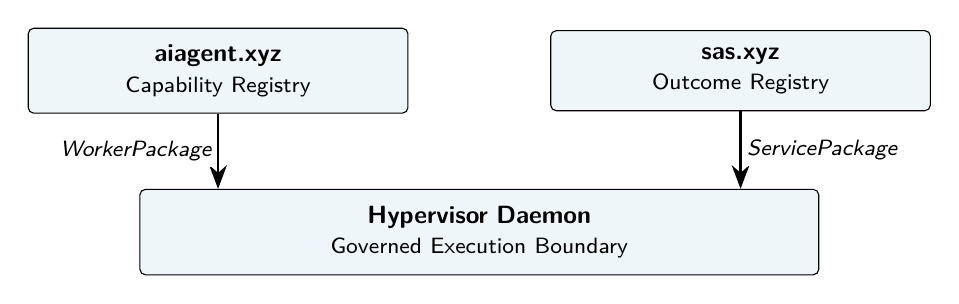
\begin{tikzpicture}[scale=1,transform shape,node distance=5mm and 9mm]
\node[ioibox,text width=44mm](a){\textbf{aiagent.xyz}\\\footnotesize Capability Registry};
\node[ioibox,right=18mm of a,text width=44mm](s){\textbf{sas.xyz}\\\footnotesize Outcome Registry};
\node[ioibox,below=15mm of $(a)!0.5!(s)$,text width=82mm](d){\textbf{Hypervisor Daemon}\\\footnotesize Governed Execution Boundary};
\draw[ioiflow](a.south)--node[ioilabel,left]{WorkerPackage}(a.south|-d.north);
\draw[ioiflow](s.south)--node[ioilabel,right]{ServicePackage}(s.south|-d.north);
\end{tikzpicture}
\end{center}

\textbf{Outcome execution, delivery, and settlement.} The ServiceEngine
governs execution of the active package, running it under a strict set
of harness profiles, model/tool bindings, authority scopes, Agentgres
projection configurations, and verification rules. The contracting cycle
operates through a secure, receipt-backed state machine:

1. \textbf{Escrow Initialization:} the buyer locks funds inside a
ServiceOrder escrow, on IOI L1 when public/economic settlement is
required or through a local/domain payment broker, work-credit ledger, or
provider account when local/domain settlement is sufficient.

2. \textbf{Execution:} the ServiceEngine executes the task, recording
all traces, observations, and tool invocations inside Agentgres.

3. \textbf{Delivery Assembly:} upon completion, the ServiceEngine
packages results, artifacts, and verification metadata into a signed
\emph{DeliveryBundle}.

4. \textbf{Delivery Acceptance:} the buyer evaluates the
\emph{DeliveryBundle} against the active Success Schema; if valid, the
escrowed funds are released.

5. \textbf{Dispute and Remediation:} if the deliverable fails
verification or violates active policy, the buyer submits a
contract-defined dispute and evidence package, triggering the selected
verifier, adjudication, and appeal path. Local/domain service contracts may resolve through
Agentgres-backed dispute state, provider accounts, or work-credit
ledgers; IOI L1 or a compatible settlement chain is used when the
ServiceOrder selected public/economic settlement, bond slashing, rights,
reputation portability, or cross-domain enforceability. Automated,
receipt-driven remediations (key revocation, developer bond slashing, or
immediate refunding) follow the verdict.

For composed services, acceptance and dispute review operate over a
\textbf{ServiceCompositionReceiptBundle} rather than raw delivery blobs,
token logs, or provider logs alone. The bundle binds composition graph
refs, routing receipts, contribution receipts, verifier refs, policy
receipts, private-data posture, dispute evidence refs, Agentgres
operation refs, and state roots. This makes nested workers, providers,
verifiers, private workspace posture, and delivery claims attributable
without making \emph{sas.xyz} the runtime, wallet, storage authority, or
contribution oracle.

\textbf{Service terminology.}

\begin{longtable}[]{@{}
  >{\raggedright\arraybackslash}p{(\linewidth - 4\tabcolsep) * \real{0.3333}}
  >{\raggedright\arraybackslash}p{(\linewidth - 4\tabcolsep) * \real{0.3333}}
  >{\raggedright\arraybackslash}p{(\linewidth - 4\tabcolsep) * \real{0.3333}}@{}}
\toprule\noalign{}
& & \\
\midrule\noalign{}
\endhead
\bottomrule\noalign{}
\endlastfoot
Term & Current Canon Definition & Relationship to Substrate \\
\textbf{ServiceModule} & Reusable execution component, deterministic
module, workflow component, or service definition invoked through a
\emph{ModuleInvocation} or \emph{StepModuleInvocation}. & Lower-level
execution unit under daemon gates; may be used inside a ServicePackage
but is not the packaged outcome itself. \\
\emph{ServicePackage} & A portable, fully configured outcome system
containing task definitions, success rubrics, and tool bindings. &
Declared on sas.xyz. Exists independently of specific runtimes or
marketplaces. \\
\emph{ServiceEngine} & The active, instantiated execution environment of
a \emph{ServicePackage} run by a Hypervisor Daemon. & Enforces harness,
model, Agentgres, and verification policies. \\
\emph{OutcomeWorkspace} & The isolated local context (sandbox) where a
\emph{ServiceEngine} executes its tasks. & Monitored by the Hypervisor
Daemon; writes state logs to Agentgres. \\
\emph{DeliveryBundle} & A cryptographically signed package containing
the final deliverables, artifact references, and execution receipts. &
Submitted to the buyer/settlement contract for acceptance
verification. \\
\emph{WorkerPackage} & A declarative, capability-oriented manifest
containing model requirements and logic (\emph{prim:*} and
\emph{scope:*}). & Registered on aiagent.xyz; represents labor capacity
rather than a contracted outcome. \\
\end{longtable}

A typical \emph{sas.xyz} outcome flow:

buyer funds or escrow locks

-\textgreater{} sas.xyz Agentgres creates ServiceOrder

-\textgreater{} OutcomeWorkspace initializes

-\textgreater{} router selects workers and compute provider

-\textgreater{} runtime assignment provisions daemon-compatible
execution

-\textgreater{} workers execute toward delivery goal

-\textgreater{} receipts, artifacts, checkpoints, and evidence are
emitted

-\textgreater{} the sas.xyz Agentgres domain admits outcome operations,
receipts, delivery state, and archive refs

-\textgreater{} idle state may seal into archive

-\textgreater{} buyer approves or disputes

-\textgreater{} the applicable settlement rail resolves triggered commitments

\hypertarget{evidence-and-artifact-roles}{%
\subsection{8.2 Evidence and Artifact
Roles}\label{evidence-and-artifact-roles}}

This section synthesizes recurring evidence roles; it is not a master schema
owner or a universal liability ladder. Canonical object/envelope,
event/receipt, Agentgres artifact-ref, marketplace, assurance, wallet, and L1
documents own exact types and wire formats.

The canonical events-and-receipts owner governs the shared
\textbf{ReceiptEnvelope} base, the exhaustive receipt-type registry,
cross-component receipt profiles, lifecycle, and assurance semantics. Domain
receipts extend that base; they do not redefine receipt identity, policy or
authority binding, Agentgres admission, assurance stages, or what proof means.
The shared base names the receipt profile and attested boundary facts and
provides separate evidence-bundle, verification, acceptance, adjudication, and
settlement refs so later states cannot be inferred from receipt existence.

\begin{itemize}
\tightlist
\item
  \textbf{Events observe.} Runtime events support streaming, debugging,
  progress, and analytics. They do not authorize effects or prove that a
  consequential crossing occurred.
\item
  \textbf{Receipts prove declared boundary facts.} A receipt binds the
  request, policy, authority decision, actor, result, evidence refs, and
  verifier coverage declared by its type. Its proof is no broader than those
  fields, evidence sources, and threat-model assumptions.
\item
  \textbf{Artifacts and payload refs preserve bytes and meaning.}
  Agentgres admits ArtifactRef/PayloadRef meaning and lifecycle; storage
  backends hold the bytes. EvidenceBundle and DeliveryBundle objects compose
  the refs needed for verification, delivery, audit, or dispute.
\item
  \textbf{Commitments and settlement envelopes are sparse projections.}
  Domains may commit selected roots for public registry, rights, reputation,
  escrow, dispute, or settlement triggers. Ordinary run history remains in its
  local/domain truth substrate.
\item
  \textbf{Analytics improves.} Cost, latency, quality, failure, benchmark,
  routing, and adoption signals improve products and the Verified Work Graph;
  analytics never substitutes for authority, receipts, or admitted truth.
\end{itemize}

TrainingReceipt, BenchmarkReceipt, EvaluationReceipt,
RoutingDecisionReceipt, ContributionReceipt, provider, custody, physical-action,
and settlement receipt families specialize those owner contracts for their
domains. A named receipt does not automatically establish completion,
liability, payment, safety, or legal fault; the applicable contract declares
the required evidence and verifier path.

Exact wire formats remain with the canonical owners. Appendix B is a
non-exhaustive synthesis for orientation and does not create a second schema
authority.
\hypertarget{the-required-receipt-sets-rrs}{%
\subsection{8.2.1 Required Receipt
Profiles}\label{the-required-receipt-sets-rrs}}

Each action, workflow, delivery, private-execution, marketplace, or
settlement contract declares the receipt and evidence profile required for
its risk class and claim. The canonical event/receipt owners govern exact
types; this whitepaper does not create separate global intent/action receipt
namespaces.

\begin{enumerate}
\def\labelenumi{\arabic{enumi}.}
\tightlist
\item
  \textbf{Coordination and completion evidence:} GoalRun, verifier-path,
  OutcomeRoom, participation and lease, frontier and claim, attempt and
  finding, WorkResult and OutcomeDelta, delivery, contribution, artifact, and
  terminal-state refs required to support a claimed workflow or outcome.
\item
  \textbf{Action-level evidence:} ActionProposal, GateResult, authority,
  policy, execution-result, normalized-observation, receipt, and artifact
  refs required for the admitted effect.
\item
  \textbf{Domain-specific evidence:} Additional custody, payment,
  external-system, physical-action, training, benchmark, routing, service,
  or settlement evidence required by the governing profile.
\end{enumerate}

Illustrative domain-specific receipt obligations

For an action to pass the Deterministic Gate and be eligible for
completion, delivery, or an implemented settlement profile, the runtime must
record the common boundary objects plus the evidence required by its target
domain:

\begin{longtable}[]{@{}
  >{\raggedright\arraybackslash}p{(\linewidth - 4\tabcolsep) * \real{0.3333}}
  >{\raggedright\arraybackslash}p{(\linewidth - 4\tabcolsep) * \real{0.3333}}
  >{\raggedright\arraybackslash}p{(\linewidth - 4\tabcolsep) * \real{0.3333}}@{}}
\toprule\noalign{}
& & \\
\midrule\noalign{}
\endhead
\bottomrule\noalign{}
\endlastfoot
Action Domain & Domain-Specific Required Evidence &
Verification Enforced \\
UI / Browser & action, target/window, visual or DOM observation, policy,
authority, and result refs & Binds the declared observable interface state
to the action; it does not prove unseen UI state. \\
Filesystem & path scope, diff or content commitment, policy, authority,
and result refs & Makes accessed paths and changes inspectable; sandbox
conformance supports the containment claim. \\
Network (Web) & destination, request/response commitment, policy,
authority, and result refs & Binds the declared target and response to the
action under the network policy. \\
Wallet / Smart Contract & exact intent, simulation, authority/approval,
transaction, external-evidence, and result refs & Binds the approved intent
and observed transaction result under the wallet contract. \\
Private-Execution Compute & custody posture, input/output commitments,
model/program ref, verifier requirements, proof/attestation refs, leakage
and declassification receipts & Binds the action to the declared
private-execution evidence profile and requires the receipt
bundle to satisfy the verifier requirements for the action class.
Substrate evidence may be TEE, FHE, MPC, ZK, deterministic replay, or
hybrid. \\
\end{longtable}

\begin{longtable}[]{@{}
  >{\raggedright\arraybackslash}p{(\columnwidth - 0\tabcolsep) * \real{1.0000}}@{}}
\toprule\noalign{}
 \\
\midrule\noalign{}
\endhead
\bottomrule\noalign{}
\endlastfoot
\textbf{Normative Invariant (The Completion Gate):}\emph{\textbf{ }}

If a run lacks evidence required by its declared profile, the runtime MUST
NOT report verified completion. It emits an explicit partial, unverified,
blocked, or failed terminal state and the applicable contract decides any
delivery, payout, dispute, or settlement consequence. \\
\end{longtable}

Additional evidence families for worker training and MoW routing

Worker Training:

\begin{enumerate}
\def\labelenumi{\arabic{enumi}.}
\tightlist
\item
  training specification and authority refs
\item
  dataset, policy-bound view, provenance, and consent refs
\item
  evaluation rubric and verifier refs
\item
  training output, cost, lineage, and receipt refs
\end{enumerate}

Benchmark Execution:

\begin{enumerate}
\def\labelenumi{\arabic{enumi}.}
\tightlist
\item
  benchmark profile and version
\item
  worker manifest and runtime refs
\item
  evaluation environment and dataset refs
\item
  score, verifier, and evidence refs
\end{enumerate}

MoW Routing:

\begin{enumerate}
\def\labelenumi{\arabic{enumi}.}
\tightlist
\item
  routing policy and version
\item
  candidate set and evidence coverage
\item
  selection reason, fee basis, and decision receipt
\item
  contribution policy and attribution refs
\end{enumerate}

Missing any required worker-training, benchmark, or routing receipt
renders the associated training result, leaderboard claim, or routing
decision economically non-enforceable.

\hypertarget{dispute-and-recourse-contracts}{%
\subsection{8.3 Dispute and Recourse
Contracts}\label{dispute-and-recourse-contracts}}

IOI does not define one universal Arbitration Core, fixed judiciary, or
deployed adjudication lane. Each ServiceOrder, marketplace transaction,
provider contract, assurance profile, or future L1 settlement profile declares
the claims that may be disputed, applicable evidence, verifier versions,
remedies, appeal path, jurisdiction, and party authorized to decide.

The default evidence order is narrow:

\begin{enumerate}
\def\labelenumi{\arabic{enumi}.}
\tightlist
\item
  validate signatures, authority and policy bindings, receipt coverage,
  ordering, inclusion, and the exact claims supported by the evidence profile;
\item
  run objective contract checks such as schema validation, tests, hashes,
  budgets, delivery conditions, or external-proof verifiers;
\item
  use constrained semantic review only where the contract declares a rubric,
  evidence boundary, abstention rule, versioned evaluator, and appeal path;
\item
  escalate ambiguity, legal interpretation, physical-world facts, insurance
  coverage, or uncovered claims to the declared human, institutional, or legal
  process.
\end{enumerate}

A receipt proves its committed fields and covered verifier result, not model
wisdom, complete context, legal fault, physical truth, or insurance coverage.
Ecosystem Assurance makes evidence and conformance posture legible but does not
adjudicate claims. A future IOI L1 may execute or anchor opted-in dispute,
escrow, bond, rights, and remedy contracts without becoming the universal
judge for local or sovereign domains.

\hypertarget{evidence-adjudication-and-typed-refusal-profiles}{%
\subsection{8.3.1 Evidence, Adjudication, and Typed-Refusal
Profiles}\label{evidence-adjudication-and-typed-refusal-profiles}}

A dispute profile may choose deterministic checks, independent verifiers,
committee or institutional review, human review, or a combination suited to
its threat model. This whitepaper does not prescribe a three-lane funnel,
model ensemble, confidence threshold, quorum algorithm, arbitration registry,
or universal dispute YAML. Exact schemas and remedies belong to the applicable
marketplace, settlement, assurance, wallet, event/receipt, and legal contract
owners.

A model, tool, provider, venue, connector, policy gate, or authority provider
may refuse a request. Refusal is a typed execution result, not automatic
developer fault, user fraud, or permission to route around policy. Any repair
opens a new proposal or route decision and re-evaluates authority, privacy,
data custody, provider trust, budget, and receipt obligations. If no admissible
route remains, the runtime records a blocker or failure and the governing
contract determines refund, incurred-cost, bond, reputation, escalation, or
terminal treatment.

\textbf{Implementation status.} Automated IOI L1 dispute adjudication,
slashing, and universal arbitration registries are speculative; no deployed
IOI L1 or fixed arbitration judiciary is claimed.
\hypertarget{hybrid-execution-model}{%
\subsection{8.3.2 Hybrid Execution Model}\label{hybrid-execution-model}}

IOI composes \textbf{probabilistic reasoning} with \textbf{deterministic
settlement}.

\begin{enumerate}
\def\labelenumi{\arabic{enumi}.}
\tightlist
\item
  \textbf{Agentic Phase: }An AI model processes fuzzy inputs (e.g.,
  "Analyze market sentiment from news feeds").
\item
  \textbf{Boundary Crossing:} Probabilistic intent collapses into a
  canonical \emph{ActionProposal} that receives a \emph{GateResult} and,
  when admitted, an \emph{ExecutionResult} or typed receipt with authority,
  policy, evidence, and replay bindings.
\item
  \textbf{Settlement Phase:} The transaction-shaped act record is passed
  into deterministic contract logic (EVM/WASM) for value transfer,
  escrow resolution, or dispute handling.
\end{enumerate}

Visual summary:


\begin{center}
\needspace{6\baselineskip}
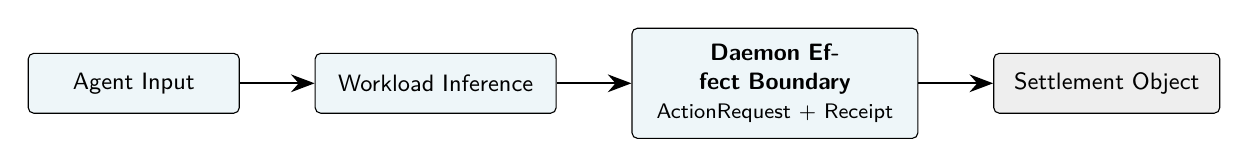
\begin{tikzpicture}[scale=0.95,transform shape,node distance=5mm and 10mm]
\node[ioibox,text width=24mm] (a){Agent Input};
\node[ioibox,right=of a,text width=28mm] (w){Workload Inference};
\node[ioibox,right=of w,text width=34mm] (f){\textbf{Daemon Effect Boundary}\\\footnotesize ActionRequest + Receipt};
\node[ioiplain,right=of f,text width=26mm] (s){Settlement Object};
\draw[ioiflow](a)--(w);\draw[ioiflow](w)--(f);\draw[ioiflow](f)--(s);
\end{tikzpicture}
\end{center}

AI handles decision-making; the Hypervisor Daemon and settlement kernel
enforce the deterministic boundary that makes the consequence
settleable. This is how Own becomes executable without making the model
itself deterministic.

\hypertarget{marketplace-neutrality-the-anti-cannibalization-invariant}{%
\subsection{8.3.3 Marketplace Neutrality: The Anti-Cannibalization
Invariant}\label{marketplace-neutrality-the-anti-cannibalization-invariant}}

A neutral MoW worker economy cannot exist if the infrastructure provider
competes with its own supply chain. If Hypervisor silently favors its own
harness adapter, worker, or service path over better declared options, it
cannibalizes marketplace workers and destroys the incentive for
developers to publish specialized intelligence.

IOI enforces Marketplace Neutrality as a core architectural invariant:

\begin{enumerate}
\def\labelenumi{\arabic{enumi}.}
\tightlist
\item
  \textbf{The Neutral Substrate:} The \textbf{Hypervisor Daemon} is the
  neutral execution substrate, not a privileged competitor; the
  \textbf{Default Harness Profile} is only the reference scaffold and
  fallback HarnessProfile, with no substrate mechanics of its own. It is
  forbidden by conformance, policy, and marketplace-neutrality doctrine
  from silently cloning or absorbing third-party worker internals into
  its default logic.
\item
  \textbf{Explainable Routing:} When Hypervisor Core, the Workflow
  Compositor, a selected HarnessProfile, MoW router, or service router
  selects a path to fulfill a task (whether the Default Harness Profile,
  an installed worker, a marketplace worker, a service outcome, a local
  module, or a hybrid composition), the routing decision MUST be
  explainable to the user and receipt trail based on declared policy:
  quality, cost, privacy, latency, required tools, installed status,
  service guarantee, trust posture, benchmark evidence, or reputation.
\item
  \textbf{Opt-In Service Redirection:} Users retain the right to run
  tasks locally via the default harness unless the task strictly
  requires licensed data, third-party authority, or hosted execution.
  Service redirection is strictly opt-in.
\item
  \textbf{No Platform Fiat:} The Default Harness Profile, a first-party
  worker, or a bundled service cannot rank itself first in marketplace
  discovery through platform fiat. Ranking must be based on measurable
  quality, reputation, policy fit, privacy, availability, and cost
  signals.
\item
  \textbf{MoW Router Neutrality:} The MoW router is subject to the same
  neutrality requirement as marketplace discovery. Routing preference
  must be based on declared policy, benchmark performance, cost,
  privacy, trust posture, installed status, or user preference. The
  runtime MUST NOT privilege first-party workers through hidden ranking
  logic, opaque bundling, or unreceipted substitution.
\end{enumerate}

\hypertarget{contribution-accounting-the-attribution-graph}{%
\subsection{8.3.4 Contribution Accounting: The Attribution
Graph}\label{contribution-accounting-the-attribution-graph}}

To ensure developers are compensated when their specialized logic is
utilized within a larger autonomous workflow, Agentgres implements
precise Contribution Accounting.

When a Planner Agent delegates a sub-task to a specialized Worker, or
utilizes a specific Tool/Model, the runtime emits a
\emph{ContributionReceipt}.

\emph{ContributionReceipts} are attribution records in MoW economics, not
automatic proof of causality, quality, value, acceptance, or payout. Payouts,
royalties, reputation updates, and routing weight follow the applicable
contract and must preserve the contribution's evidence, assurance,
acceptance, adjudication, and settlement stage. Ordinary Goal Space Work
Credits meter managed product usage; they are not distributed to contributors.

The \emph{ContributionReceipt} records:

\begin{enumerate}
\def\labelenumi{\arabic{enumi}.}
\tightlist
\item
  \textbf{The Contributor Identity} (\emph{ai://workers.xyz})
\item
  \textbf{The Contribution Type} (e.g., verification, generation,
  planning, tool usage)
\item
  The Input and Output Artifact References
\item
  \textbf{The Quality Delta} (the measurable improvement the worker
  provided to the workflow)
\item
  The Reward Basis and License Terms
\end{enumerate}

For MoW settlement, the \emph{ContributionReceipt} MAY also record:

\begin{enumerate}
\def\labelenumi{\arabic{enumi}.}
\tightlist
\item
  routing\_decision\_ref
\item
  sparse\_worker\_category
\item
  benchmark\_profile\_ref
\item
  verifier\_worker\_ref
\item
  failure\_or\_dispute\_status
\item
  downstream\_outcome\_ref
\end{enumerate}

These receipts form an \textbf{Attribution Graph}, the contribution and
payout projection of the broader Verified Work Graph, within the relevant
Agentgres domains. They support:

\begin{enumerate}
\def\labelenumi{\arabic{enumi}.}
\tightlist
\item
  \textbf{Usage and Payout Accounting:} Driving approved fiat,
  stablecoin, IOI, credit, royalty, or other payout rails. IOI L1 receives
  only the selected public, economic, rights, reputation, or dispute
  commitments that require it.
\item
  \textbf{Reputation Updates:} Feeding quality ledgers so that highly
  effective workers organically rise in marketplace rankings based on
  proven outcomes, not marketing.
\item
  \textbf{Dispute Traceability:} Allowing Arbitrators to pinpoint
  exactly which node in a multi-agent supply chain failed, ensuring
  liability falls only on the responsible party.
\end{enumerate}

The IOI protocol doctrine is strict: The platform must route
intelligence, not absorb it.

\textbf{Incentive-Compatible Contribution Without IP Disclosure:} IOI
does not require developers to open-source their models, weights,
prompts, or datasets in order for the network to improve. A developer
who creates a superior verification Worker, planning Worker,
data-curation Worker, or domain-specialist Worker can expose it through
a manifest and policy-bound interface while retaining the underlying IP.
Contribution accounting allows such Workers to receive attribution and
compensation when routed into larger workflows, synthetic-data
pipelines, or execution graphs. The network improves because useful
intelligence is economically routable, not because participants are
assumed to share gradients without compensation.

\hypertarget{economics-pricing-verifiable-work}{%
\subsection{8.4 Economics: Pricing Verifiable
Work}\label{economics-pricing-verifiable-work}}

This section specifies the economic boundary of the IOI product and
protocol stack. \textbf{Product surfaces monetize useful autonomous work,
managed execution, distribution, governed trust, verified outcomes,
routing value, private managed posture, and value movement.} Verification,
authority, receipts, and routine Agentgres operations are bundled substrate
and must remain independently inspectable rather than becoming toll booths.

The open/protected split follows the trust boundary. The \textbf{open
verification layer} includes protocol contracts, receipt schemas, authority
envelopes, portable memory format, adapter contracts, SDK interfaces, and
conformance fixtures required to verify IOI's honesty offline. The
\textbf{protected local runtime layer} may include the local Hypervisor core,
Agentgres runtime implementation, wallet authority daemon, and provider
adapter runtime. The \textbf{proprietary network/operations layer} may
monetize hosted ioi.ai, managed compute, private runtime, routing and
placement intelligence, cross-party Verified Work Graph aggregation,
marketplace reputation, billing, procurement, support, and enterprise or
compliance operations.

\textbf{WorkCredit} is the broad product usage and budget abstraction for
managed autonomous work. It may meter model, runtime, provider, connector,
private-workspace, storage, replay, Foundry, Automation, conductor,
marketplace, service, verifier, or audit cost when those create managed
product cost. Work Credits are bounded and non-transferable product
credits, not cash, Worker payout, pooled provider seats, a claim on
provider tokens, the IOI protocol token, or necessarily the final
settlement asset. Token or BME mechanics follow only after verified-work
demand, marketplace liquidity, and real public-settlement needs exist.

The canonical commercial shape is \textbf{one Goal Space with two
supply lanes}:

\begin{itemize}
\tightlist
\item
  \textbf{Goal Space subscription:} persistent conductor and goal state,
  portable memory, policy, receipts, replay, collaboration, ordinary
  support, provider-neutral Auto routing, and a bounded monthly grant of
  Work Credits.
\item
  \textbf{Additional managed work:} Work Credit top-up, opt-in overage,
  or committed-spend drawdown for heavy multi-session, model, compute,
  storage, connector, verifier, training, or background work.
\item
  \textbf{Network / Open participation:} a separately bounded
  NetworkGoalBudget, bounty, procurement cap, or \emph{sas.xyz}
  ServiceOrder for independent Workers, verifiers, services, challenges,
  and settlement.
\item
  \textbf{Enterprise / Private:} seats plus committed managed-work spend,
  customer-boundary or private runtime, reserved capacity,
  administration, governance, audit, retention, residency, service level,
  and support.
\end{itemize}

One logical Hypervisor domain may schedule many Workers across machines,
clouds, model providers, and failure domains while remaining one
authority, truth, and settlement domain. Node count is not the SKU.
Same-domain 1--N orchestration may use GoalRun and OutcomeRoom
coordination under the bounded Work Credit budget, but it does not
manufacture multi-party federation. Independent participation is opt-in,
explicitly admitted, affiliation-visible, and separately funded.

Three product controls remain orthogonal. \textbf{Execution/custody}
selects Standard or Private posture; \textbf{contributor scope} selects
My Workers, Organization, or Network / Open; and \textbf{placement}
selects local, customer infrastructure, a chosen provider, or
Hypervisor-selected placement. Contributor scope never declassifies data,
widens authority, relaxes retention or export policy, or changes custody
promises. Every candidate satisfies the intersection of Goal Space and
home-domain policy or remains ineligible.

\textbf{Managed worker pricing} may include:

\begin{enumerate}
\def\labelenumi{\arabic{enumi}.}
\tightlist
\item
  install or license fee;
\item
  per-invocation fee;
\item
  warm runtime subscription;
\item
  persistent runtime subscription;
\item
  zero-to-idle restore fee;
\item
  storage/archive fee;
\item
  model/provider usage;
\item
  compute provider fee;
\item
  verifier/evaluator fee;
\item
  worker author royalty;
\item
  marketplace/distribution fee or explicitly triggered public-settlement
  fee.
\end{enumerate}

Settlement should remain receipt-bound through
\emph{WorkerInvocationReceipts}, \emph{RuntimeAssignmentReceipts},
\emph{ComputeSessionReceipts}, \emph{StorageArchiveReceipts},
\emph{RestoreReceipts}, \emph{EvaluationReceipts},
\emph{ContributionReceipts}, and \emph{SettlementReceipts}.

\hypertarget{the-economic-shift-paying-for-outcomes-not-just-compute}{%
\subsection{8.4.1 The Economic Shift: Paying for Outcomes, Not Just
Compute}\label{the-economic-shift-paying-for-outcomes-not-just-compute}}

In the commodity inference model, users pay for compute cycles. Value
accrues to hardware, not to the orchestration or verification of work.

In the Web4 IOI model, users can purchase governed work or contract for
an accepted outcome under declared evidence, verification, acceptance,
remedy, and settlement terms. A receipt binds attributable boundary
facts; it does not make an output correct or payable by itself. Where a
ServiceOrder or escrow is used, release follows the implemented contract's
verification, acceptance, adjudication, and appeal semantics.

This mechanism establishes a Market for Verifiable Work, effectively
decoupling the computational cost of inference from the economic value
of the executed task.

Developer Economics

IOI captures the economic sweet spot between Services and Software.

\begin{itemize}
\tightlist
\item
  \textbf{Services} have high value (doing the work) but low margins
  (humans don't scale).
\item
  \textbf{Software} has low value (just a tool) but infinite margins
  (zero marginal cost of replication).
\end{itemize}

Service-as-a-Software combines the utility of a service with the
replicability of governed Worker and Service packages. Developers may
publish versioned capability once and earn invocation, license, service,
or contribution revenue under declared terms without operating every
runtime themselves. Receipt-bound metering and contribution accounting
make that asset class economically legible.

\hypertarget{the-liquidity-orchestration-layer-protocol-revenue}{%
\subsubsection{8.4.1.1 The Liquidity \& Orchestration Layer (Product and
Network Operations Revenue)}\label{the-liquidity-orchestration-layer-protocol-revenue}}

IOI products and network operations sustain themselves by monetizing useful
outcomes, managed execution, distribution, governed trust, routing value,
assurance, support, and value movement---not by extracting rent from local
execution or substrate primitives.

1. Provider Orchestration as Product / Network Operations Revenue

Whenever a user\textquotesingle s local node lacks the precise
computational resources (for example VRAM, storage durability, latency,
or confidential-compute posture) to run a Worker Manifest, Hypervisor
may deploy the workload through a direct provider integration or a
candidate source such as \emph{decentralized.cloud}. The pricing boundary
follows the value Hypervisor actually supplies:

\begin{itemize}
\tightlist
\item
  \textbf{Direct local or direct self-managed BYO:} no percentage fee on
  provider spend. Subscription, collaboration, governance, support, or
  control-plane value may still be priced explicitly.
\item
  \textbf{Pinned or BYO-through-Hypervisor lifecycle:} a visible
  adapter/orchestration, credential-brokerage, custody, restore,
  monitoring, support, or audit fee is legitimate when Hypervisor actually
  performs that work. It is not an optimized-routing fee.
\item
  \textbf{Optimized placement:} a routing or procurement fee is
  legitimate only when Hypervisor creates real comparison, procurement,
  failover, reconciliation, or aggregation value and emits challengeable
  placement/routing evidence.
\item
  \textbf{Managed infrastructure:} when IOI or a partner is
  provider-of-record, Work Credits, managed-runtime margin, reserved
  capacity, and support pricing are legitimate because the provider bears
  procurement or operational risk.
\end{itemize}

2. Swap Spreads \& Liquidity (Wallet Revenue)

The user-facing \emph{wallet.network} treats exchange as a first-class
authority action. Route candidates may come from
\emph{decentralized.exchange}, direct pools, routers, solvers,
aggregators, or user-specified paths. Liquidity is provided by venues
and pools, not by wallet.network itself. wallet.network evaluates risk,
policy, simulation, approval, signing, and receipts, and may capture a
transparent convenience or route fee where policy, disclosure, and local
law permit.

\hypertarget{stakeholder-alignment}{%
\subsection{8.4.2 Stakeholder Alignment}\label{stakeholder-alignment}}

This model aligns incentives across the core stakeholders of the
automated economy:

\begin{itemize}
\tightlist
\item
  \textbf{Users (Demand):} Purchase verified outcomes. They utilize
  ServiceOrders, outcome escrows, and delivery acceptance rules to make
  payout conditional on successful, receipt-backed work under the
  declared contract. They
  maintain data sovereignty because protected state is governed by
  Agentgres artifact refs, wallet.network authority, and Private
  Workspace/cTEE posture rather than hidden developer servers.
\item
  \textbf{Providers (Supply):} Earn revenue for providing compute,
  storage, readiness, and confidential/private execution posture,
  fulfilling offloaded sessions through local, cloud, DePIN,
  TEE/confidential-compute, cTEE/private workspace, or customer-owned
  provider lanes.
\item
  \textbf{Developers (Creators):} Earn royalties when their
  WorkerPackages, ServicePackages, connectors, evaluators, or ontology
  assets are invoked under their package/license terms, without ever
  incurring idle server costs or exposing proprietary payloads beyond
  the selected custody profile.
\item
  \textbf{Payment Brokers / Work-Credit Issuers (Liquidity):} Optional
  bridges between product billing and protocol or provider settlement.
  They may account for fiat subscriptions, enterprise invoices, prepaid
  credits, stablecoin reserves, or marketplace escrows, but wallet.network
  or the applicable local/domain authority still authorizes budgets, grants,
  revocation epochs, and receipts. They
  can provide working capital for provider sessions without forcing
  routine local/domain operations onto a public chain.
\item
  \textbf{Future dispute operators or verifiers:} An implemented public
  dispute profile may pay explicitly contracted verification or resolution
  fees. No live IOI L1 arbitration-node market is asserted.
\end{itemize}

\hypertarget{metered-work-credit-model-the-micro-split-settlement}{%
\subsection{8.4.3 Metered Work Credits and Itemized
Charges}\label{metered-work-credit-model-the-micro-split-settlement}}

Work Credits debit a product usage budget; they do not force every run into
one universal settlement formula. Charges are itemized only when the
corresponding value or cost exists:

\begin{enumerate}
\def\labelenumi{\arabic{enumi}.}
\tightlist
\item
  \textbf{Provider pass-through:} Customer- or product-borne model,
  compute, API, storage, network, or other provider cost, shown separately
  from IOI fees.
\item
  \textbf{Product/control-plane subscription:} Hypervisor, ioi.ai,
  collaboration, governance, memory, Provenance, support, or enterprise
  product value.
\item
  \textbf{Adapter/lifecycle fee:} Visible credential-brokerage,
  provisioning, lease, snapshot, restore, monitoring, teardown, custody,
  audit, or support work for a pinned or BYO venue.
\item
  \textbf{Managed-capacity charge:} Provider-of-record compute, reserved
  capacity, private managed runtime, or operational/support margin.
\item
  \textbf{Optimized-routing fee:} Actual comparison, procurement,
  matching, failover, reconciliation, or aggregation value supported by
  challengeable routing or placement evidence.
\item
  \textbf{Marketplace/license/royalty charge:} Declared distribution,
  procurement, licensing, worker, service, package, connector, evaluator,
  ontology, or other eligible contribution value.
\item
  \textbf{Triggered public settlement/dispute charge:} Fees for an
  implemented registry, rights, reputation, bond, escrow, dispute,
  governance, or settlement contract only when that public boundary is
  selected.
\end{enumerate}

The accountable charge is the sum of supplier model/accelerator/compute
cost; sandbox, storage, connector, environment, and replay cost; external
Worker, verifier, or service cost; and the declared IOI managed-work and
orchestration charge. The user-facing rate card may normalize those
inputs, but the receipt ledger preserves the actual Worker composition,
model/provider/endpoint and route, price schedule, token or compute
categories where available, attempted and billed fallbacks,
verifier/escalation reason, supplier or broker cost class, IOI fee basis,
adjustments or refunds, and total Work Credits. Customer BYOK, BYOA,
customer-cloud, self-hosted, or local execution is not charged again for
supplier cost already borne by the customer.

Auto / 1-of-N, Pinned, and Compare / N-of-N are execution policies, not
plan tiers. Auto may use a verified cheap-first cascade and escalate only
when its declared acceptance path fails. Pinned fails closed on an
ineligible or unavailable route unless qualified fallback was expressly
authorized. Compare quotes and accounts for every admitted attempt,
verifier, and synthesis leg. Expensive or externally procured work exposes
a quote or cap before commitment.

A workflow node, receipt, authority check, connector grant, policy decision,
or Agentgres write is not independently billable merely because it exists.
Only optimized placement or another paid routing/procurement decision should
mint a RoutingDecisionReceipt; ordinary pinned-provider lifecycle work uses
provider-operation and billing evidence.

\textbf{Self-directed economics.} A local or direct self-managed run has no
external provider pass-through or percentage-of-provider-spend fee. If it
uses no licensed supply, managed service, public anchor, escrow, or dispute
path, those buckets are absent as well. Sovereignty is a first-class route,
not a discounted version of mandatory network escalation.\\

\hypertarget{goal-space-subscription-work-credits-and-separate-network-funding}{%
\subsubsection{8.4.3.1 Goal Space Subscription, Work Credits, and
Separate Network
Funding}\label{goal-space-subscription-work-credits-and-separate-network-funding}}

Mass adoption must not require retail users to purchase tokens, manage a
wallet, assemble model subscriptions, or understand provider billing.
ioi.ai therefore sells one seat-like Goal Space outcome product rather
than separate single-node and network-node subscriptions or a bundle of
named-human foundation-model plans.

The user pays fiat or an approved enterprise billing rail for the
persistent conductor, goal/account state, portable memory, policy,
receipts, replay, collaboration, ordinary support, and a bounded monthly
Work Credit grant. Additional managed work uses top-up, opt-in overage,
or committed spend. The allowance is sized from observed cost of goods,
route mix, acceptance rate, concurrency, context, verification, and
support load rather than by adding together retail chat-plan prices or
promising unlimited multi-worker burn.

Product billing and economic settlement remain distinct:

\begin{enumerate}
\def\labelenumi{\arabic{enumi}.}
\tightlist
\item
  \textbf{Product funding:} The Goal Space plan issues a bounded,
  non-transferable Work Credit allowance and records top-up, overage, or
  committed-spend consent.
\item
  \textbf{Managed usage:} Work Credits debit model, runtime, connector,
  storage, Worker, verifier, and conductor costs under the disclosed rate
  card and itemized usage ledger.
\item
  \textbf{Independent participation:} Opening contributor scope to
  Network / Open uses a separate NetworkGoalBudget, bounty, procurement
  cap, or ServiceOrder. It never silently consumes the ordinary seat
  allowance.
\item
  \textbf{External payout:} Eligible providers, Workers, services,
  verifiers, and contributors settle separately through fiat, stablecoin,
  IOI, or another approved rail under the applicable contract,
  jurisdiction, authority, assurance, acceptance, and dispute posture.
  Agentgres admits the corresponding evidence and ledger refs.
\end{enumerate}

The Goal Space subscription may fund same-domain managed execution and
IOI's disclosed seed supply because those remain one product/operator
lane. Genuine independent labor is opt-in and separately funded. Work
Credits are therefore never a vague pro-rata payout pool. A
ContributionReceipt supplies attribution evidence; payout eligibility
requires the declared verification, acceptance, adjudication, and
settlement path. The economically relevant unit is accepted or otherwise
contract-eligible contribution, not raw model tokens or receipt count.

\hypertarget{supply-side-incentives-package-license-fee-routing}{%
\subsection{8.4.4 Supply-Side Incentives: Package/License Fee
Routing}\label{supply-side-incentives-package-license-fee-routing}}

IOI introduces package/license-anchored fee routing to sustainably
monetize open-source workers, proprietary tools, service packages,
ontology packs, evaluators, and connector surfaces.

\begin{itemize}
\tightlist
\item
  \textbf{Mechanism:} A signed manifest and its declared license/right record
  identify eligible recipients, contribution terms, and
  Agentgres-governed package/artifact refs. No optional token becomes the
  universal canonical recipient merely by existing.
\item
  \textbf{Enforcement:} When a session invokes a WorkerPackage,
  ServicePackage, connector, evaluator, or licensed artifact, the
  applicable product, marketplace, or settlement rail checks the declared
  package/license terms. Where the contract and jurisdiction support it, the
  rail calculates eligible royalties from receipt-backed metering and routes
  them to the declared recipients.
\item
  \textbf{Impact:} This supports a \textbf{"Royalty-on-Execution"} model
  rather than only "Royalty-on-Access." Supply may be open, protected, or
  proprietary under its license and custody profile; verification must not
  depend on pretending that a compiled artifact makes source visible.
\end{itemize}

\hypertarget{contribution-accounting-marketplace-neutrality}{%
\subsection{8.4.5 Contribution Accounting \& Marketplace
Neutrality}\label{contribution-accounting-marketplace-neutrality}}

The core economic problem of an ``Internet of Intelligence'' is
cannibalization. If the platform silently routes around specialized
workers, clones worker internals into default behavior, or hides
first-party preference behind opaque ranking, it destroys the incentive
for developers and service providers to publish specialized
intelligence.

IOI prevents this through strict Marketplace Neutrality and Contribution
Accounting. This economic layer ensures that whenever intelligence is
shared, it is attributed and compensated, protecting the MoW worker
economy.

\begin{enumerate}
\def\labelenumi{\arabic{enumi}.}
\tightlist
\item
  \textbf{The Anti-Cannibalization Invariant:} Hypervisor, the Default
  Harness Profile, MoW routers, marketplace surfaces, and service
  routers must not silently clone, appropriate, or hide third-party
  worker, service, dataset, evaluator, or tool contributions. If a run
  utilizes a specialized tool, dataset, worker, service, evaluator, or
  licensed artifact to fulfill an intent, the runtime MUST emit a
  \emph{ContributionReceipt} or domain-specific usage receipt.
\item
  \textbf{The }\emph{ContributionReceipt}\textbf{:} This attributable
  artifact records the declared identity that contributed intelligence (the
  \emph{contributor\_id}), \emph{how} it was used (e.g., planning,
  verification, tool execution), and the \emph{quality\_delta} (the
  measurable improvement it provided to the final outcome).
\item
  \textbf{The Attribution Graph:} These receipts form an attribution
  projection of the Verified Work Graph within the Agentgres domain. When a
  user pays for a successful outcome, an applicable product, marketplace, or
  settlement rail may use the graph to calculate eligible royalties, Work
  Credit accounting, or payouts according to the declared contribution,
  license, authority, and jurisdictional policy for that task.
\item
  \textbf{Reputation as an Asset:} Even in ``free'' or local executions
  where no tokens change hands, \emph{ContributionReceipts} may update a
  reputation root, marketplace projection, or local quality ledger. This
  lets Workers, services, evaluators, datasets, and packages rise in
  discovery based on attributed use and evaluated outcome evidence,
  rather than platform fiat or marketing spend. The receipt alone does
  not prove utility or acceptance.
\end{enumerate}

This shifts the economic model from zero-sum competition to composable
collaboration. Developers are economically incentivized to publish
small, hyper-specialized workers because receipted contributions can become
eligible for royalties, reputation, or routing weight under the applicable
contract instead of disappearing inside a larger workflow, service order, or
MoW labor graph.

\hypertarget{escalation-economics}{%
\subsection{8.4.6 Escalation Economics}\label{escalation-economics}}

An implemented public ServiceOrder dispute profile should prevent abuse
through explicit anti-griefing bonds and challenge windows. The following is
a target contract shape, not a claim that IOI L1, a live Arbitration Lane, or
its bond economy is deployed.

Liability Binding \& Target Enforcement Status

The IOI economic ladder relies on the settlement schema binding the
execution artifacts to real capital.

\begin{itemize}
\tightlist
\item
  \textbf{Minimal Target Invariant:} A bonded on-chain escrow profile
  must bind to \emph{(session\_id, policy\_hash, receipt\_root)}. A
  dispute under that profile must present a challenged receipt and valid
  inclusion evidence against the committed root.
\item
  \textbf{Current Enforcement Status:} Speculative. No IOI L1 deployment,
  validator set, public escrow/bond contract, payment settlement, or
  production dispute lane is asserted by the current architecture canon.
\item
  \textbf{Candidate Enforcement:} Any future automated remedy or slashing
  path must bind exact contract terms, evidence, authority, verifier,
  challenge, and appeal semantics rather than treating a policy hash or
  receipt root alone as proof of breach.
\end{itemize}

Escalation Parameterization

A candidate public arbitration profile may parameterize the following
controls, with values set only by the governance and contract profile that
actually deploys them:

\begin{enumerate}
\def\labelenumi{\arabic{enumi}.}
\item
  \textbf{Challenge Bonds (Base Bond Function):} \emph{Base\_Bond =
  max(Task\_Value * Risk\_Multiplier, Minimum\_Floor)}. If a User
  rejects a Provider\textquotesingle s deliverable (or if a Provider
  contests a User\textquotesingle s refusal to pay), the escalating
  party MUST post this escalation bond.
\item
  \textbf{Superlinear Cost Curve (Lane Multipliers):} Escalation bonds
  increase geometrically with the arbitration tier. Moving from
  deterministic objective checks (Lane 1) to AI semantic verification
  (Lane 2) to Human Review (Lane 3) incurs a geometric cost increase:

  EscalationBond\_lane\_n = BaseBond × LaneMultiplier\^{}n

  where n is the escalation lane index and LaneMultiplier is a
  governance parameter.
\item
  \textbf{Burn/Return Policy:} A mathematically defined percentage of
  the loser's dispute bond is burned. This creates a negative-sum game
  for frivolous disputes, ensuring Arbitration is only invoked when a
  party has high confidence in their cryptographic evidence.
\item
  \textbf{Challenge Windows \& Anti-Griefing Caps:} Dispute windows are
  strictly defined in epochs (e.g., defaulting to 24 hours for
  asynchronous disputes), alongside hard caps on the maximum allowable
  escalations per session or per epoch to prevent griefing loops.
\item
  \textbf{Pre-funding:} The escalating party MUST pre-fund the
  incremental compute and gas required by the Arbitration Nodes to run
  the verification trace.
\end{enumerate}

\hypertarget{the-embodied-autonomous-labor-profile}{%
\subsection{8.5 Embodied Runtime and Physical Action
Safety}\label{the-embodied-autonomous-labor-profile}}

\textbf{Implementation status: speculative beyond narrow package admission.}
The current worker-package install path can require vertical-pack,
physical-action-policy, safety-envelope, and emergency-stop references for a
package declaring \emph{physical\_action}. That admission check is not a live
robot-fleet runtime, certified local controller, two-speed mission path,
segment-commitment implementation, or completed actuator boundary; none of
those target capabilities is claimed as built.

Embodied autonomous systems (such as warehouse robots, humanoid devices,
delivery drones, and automated manufacturing systems) use
\textbf{Embodied Runtime}, the Hypervisor runtime profile for live physical
domains. It owns robot/fleet identity, controller bindings, sensor and
actuator registries, world state, command queues, telemetry, physical replay,
recovery, and operator handoff while reusing worker manifests,
wallet.network authority, Agentgres, and AIIP boundaries.

\textbf{Two-speed embodied architecture.} Physical autonomy separates
mission-level governance from high-frequency control:

\begin{enumerate}
\def\labelenumi{\arabic{enumi}.}
\item
  The \textbf{governance and intelligence plane} grounds the mission,
  negotiates ontology and action semantics, plans and simulates, classifies
  risk, budgets resources, obtains applicable authority, selects supervision
  and recovery policy, issues bounded mission envelopes, evaluates segment
  summaries, and pauses, revokes, or course-corrects at mission checkpoints.
  Goal Kernel, the Hypervisor Daemon, local/domain governance,
  wallet.network where portable delegated or high-risk authority is required,
  and Agentgres operate at this slower boundary.
\item
  The \textbf{certified local control and safety plane} owns controller-rate
  perception and actuation, controller-local invariants, watchdog and
  heartbeat enforcement, command clipping or denial, local emergency stop,
  safe-stop transitions, and immediate exception capture. It is independently
  enforceable from the model policy and operates only inside the admitted
  mission envelope and its stricter local \textbf{SafetyEnvelope}.
\end{enumerate}

The slow plane issues a \textbf{PhysicalMissionControlEnvelope} binding the
mission and target robots, zones, controller and version, physical-action
policy, safety envelope, authority and revocation epoch, supervision and
emergency-stop policy, maximum envelope age, heartbeat and failsafe posture,
segment-commitment cadence, resource budget, and recovery/incident rules. A
mission envelope amortizes governance; it does not authorize arbitrary local
setpoints or weaken the local controller's veto.

The local plane records each bounded interval as a
\textbf{LocalControlSegment}. It may summarize ordinary control ticks with
command, sensor, controller-state, and telemetry roots in a
\textbf{PhysicalActionSegmentCommitmentReceipt}, but a segment aggregate must
not hide command denials, safety-envelope violations, heartbeat failures,
emergency stops, operator handoffs, or incidents. Those material exceptions
emit immediate receipts and force the declared local stop, deny, or handoff
behavior.

Remote model calls, Goal Kernel turns, wallet.network round trips, Agentgres
admission, AIIP exchange, and public settlement are forbidden dependencies in
a servo or motor-control loop. Their latency may delay the next mission,
checkpoint, or segment admission; it must not delay the controller's local
safety veto, watchdog, or emergency stop.

However, physical actions cannot be treated like normal software
actions. A physical effect cannot be assumed to roll back or become safe
because a digital state transition was reverted. Every actuator-bearing
mission or effect therefore declares a recovery class:
\emph{replayable}, \emph{checkpointable}, \emph{compensatable},
\emph{reconciliation\_required}, or \emph{non\_retryable}. Unknown commit
state, ambiguous physical outcome, and non-retryable action fail closed into
reconciliation or incident handling instead of blind replay.

To mitigate physical execution risks, actuator-affecting work must be
classified as \emph{physical\_action} and pass an independently enforceable
\textbf{PhysicalActionPolicy} and \textbf{SafetyEnvelope}. Current sensor
evidence and the issued command/result bindings are recorded through
\textbf{SensorEvidenceReceipt} and \textbf{ActuatorCommandReceipt} refs
admitted by Agentgres. These receipts make the digital record inspectable;
they do not by themselves prove that a real-world command was safe, issued,
stopped, or completed.


\begin{center}
\needspace{6\baselineskip}
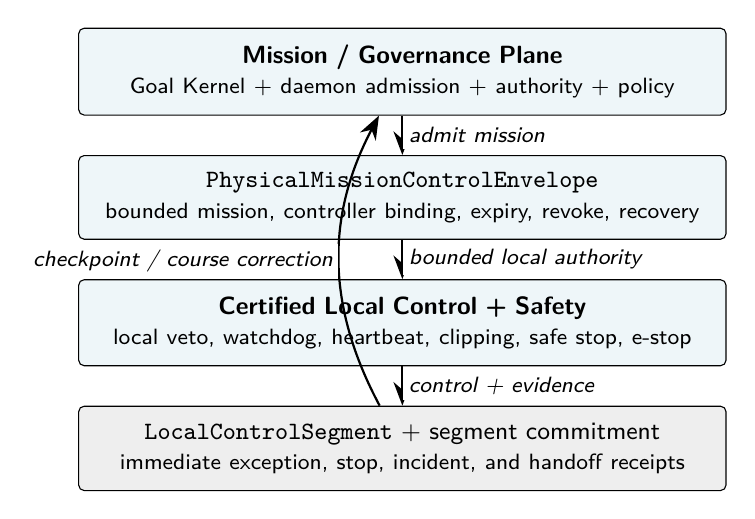
\begin{tikzpicture}[scale=1,transform shape,node distance=5mm and 9mm]
\node[ioibox,text width=78mm](g){\textbf{Mission / Governance Plane}\\\footnotesize Goal Kernel + daemon admission + authority + policy};
\node[ioibox,below=of g,text width=78mm](m){\texttt{PhysicalMissionControlEnvelope}\\\footnotesize bounded mission, controller binding, expiry, revoke, recovery};
\node[ioibox,below=of m,text width=78mm](l){\textbf{Certified Local Control + Safety}\\\footnotesize local veto, watchdog, heartbeat, clipping, safe stop, e-stop};
\node[ioiplain,below=of l,text width=78mm](s){\texttt{LocalControlSegment} + segment commitment\\\footnotesize immediate exception, stop, incident, and handoff receipts};
\draw[ioiflow](g)--node[ioilabel,right]{admit mission}(m);
\draw[ioiflow](m)--node[ioilabel,right]{bounded local authority}(l);
\draw[ioiflow](l)--node[ioilabel,right]{control + evidence}(s);
\draw[ioiflow](s) to[bend left=28] node[ioilabel,left]{checkpoint / course correction}(g);
\end{tikzpicture}
\end{center}

\textbf{Physical safety and human supervision as authority primitives.}
Human oversight is not merely a notification feature.
\textbf{EmergencyStopAuthority} and \textbf{HumanSupervisionPolicy} are
physical-action safety objects whose holders, scopes, channels, latency,
test posture, and revocation epoch bind to wallet.network or other applicable
authority records. Their safety semantics remain owned by Physical Action
Safety.

The \textbf{EmergencyStopAuthority} is a high-priority authority and safety
contract with independently operable local channels. It must not require a
remote cryptographic round trip before the local stop path can act. If a
physical boundary is breached, or
if a human supervisor triggers an emergency stop through an approved
channel such as a local button, workstation, facility system, app, web,
voice-supervisor path, or API, the local safety controller or approved
adapter retains the final real-time veto and drives the affected actuator
domain into its declared fail-closed state. The daemon stops or denies the
relevant command path, revokes or invalidates affected leases, and records
incident evidence. wallet.network belongs to mission admission, authority,
spend, scope, and revocation; it is not placed in the millisecond actuator
loop. Hardware interlocks and facility safety systems remain part of the
safety envelope.

Any safety-envelope violation, emergency stop, sensor disagreement,
actuator failure, supervision failure, policy violation, or disputed
physical outcome must open a \textbf{PhysicalActionIncident}. Incidents
bind involved intents, sensor evidence, actuator receipts, emergency-stop
state, remediation policy, and dispute refs inside Agentgres before any
marketplace, insurer, venue, or L1 settlement path may treat the event as
resolved. The L1 is not the safety controller; it receives only selected
rights, insurance, settlement, dispute, reputation, or public
accountability commitments after the daemon and Agentgres have recorded
the operational incident.

\textbf{Embodied-labor safety objects.}

\begin{longtable}[]{@{}
  >{\raggedright\arraybackslash}p{0.24\linewidth}
  >{\raggedright\arraybackslash}p{0.23\linewidth}
  >{\raggedright\arraybackslash}p{0.22\linewidth}
  >{\raggedright\arraybackslash}p{0.21\linewidth}@{}}
\toprule\noalign{}
& & & \\
\midrule\noalign{}
\endhead
\bottomrule\noalign{}
\endlastfoot
Architecture Object & Description & Substrate Mapping & Security /
Execution Enforced \\
\textbf{Physical\allowbreak{}Mission\allowbreak{}Control\allowbreak{}Envelope} & Bounded mission contract binding
targets, controller/version, policies, authority/revocation, expiry,
heartbeat/failsafe, supervision, segment cadence, resources, and recovery. &
Issued through mission-level governance and daemon admission; referenced by
the local control bridge and Agentgres mission truth. & Bounds what the local
controller may attempt without entering the controller-rate loop. \\
\textbf{Local\allowbreak{}Control\allowbreak{}Segment} & One bounded local-control interval under a
specific mission envelope, controller version, and revocation epoch. & Owned
by Embodied Runtime and summarized through command, sensor, telemetry,
exception, and commitment refs. & Keeps high-rate control local while making
bounded intervals inspectable and revocable at checkpoints. \\
\textbf{Physical\allowbreak{}Action\allowbreak{}Policy} & Standardized ruleset defining velocity,
torque, force limits, and allowed operational coordinates. & Registered
as a mission-admission policy object with Agentgres/domain policy refs and an
independently enforceable local binding. & Requires the local safety path to
deny, clip, stop, or hand off commands outside declared bounds. \\
\textbf{Safety\allowbreak{}Envelope} & Real-time virtual barrier mapping physical
coordinates, LiDAR clearance, and safe operating zones. & Enforced by an
independent local safety boundary, controller, approved adapter, or facility
safety system, with daemon and Agentgres bindings. & Can deny, clip, stop,
or require handoff when a proposed command exceeds the envelope. \\
\textbf{Emergency\allowbreak{}Stop\allowbreak{}Authority} & High-priority authority and safety contract
for immediate scoped stop and revocation of affected command paths, including
independently operable local channels. &
Declared holders, trigger channels, maximum latency, test state, and
revocation epoch bound to applicable authority records. & The local safety
path stops affected actuators and the daemon invalidates relevant leases;
it does not require killing the entire daemon or clearing unrelated sessions. \\
\textbf{Human\allowbreak{}Supervision\allowbreak{}Policy} & Rules defining required check-in
intervals, operator visual verification, and step-up confirmations. &
Linked as a \emph{RequireApproval} gate on high-risk physical tasks. &
The local plane enters its declared safe state while mission-level governance
requests approval or operator handoff; no remote approval is awaited inside
the control loop. \\
\textbf{Sensor\allowbreak{}Evidence\allowbreak{}Receipt} & Receipt binding camera, LiDAR, IMU, or
other sensor snapshot hashes, capture time, confidence, artifacts, and
redaction policy. & Saved through Agentgres with EvidenceBundle and
ArtifactRef links. & Records the declared sensor evidence used to justify
or audit execution under stated capture and verifier assumptions. \\
\textbf{Actuator\allowbreak{}Command\allowbreak{}Receipt} & Receipt binding physical command hash,
actuator ref, issuing daemon, authority ref, safety envelope ref, sensor
evidence receipt refs, and command result. & Committed directly to
Agentgres as a specialized physical-action receipt. & Records the digital
command/result binding; it does not independently prove safe or faithful
real-world motion. \\
\textbf{Physical\allowbreak{}Action\allowbreak{}Segment\allowbreak{}Commitment\allowbreak{}Receipt} & Receipt binding a local
control interval, controller/version, mission envelope, command and sensor
roots, exception refs, start/end state, and declared result. & Emitted at the
mission's segment cadence and admitted with the embodied replay record. &
Summarizes ordinary ticks without replacing immediate violation, stop,
incident, or mission-level reconciliation receipts. \\
\textbf{Liability\allowbreak{}Claim\allowbreak{}Route} & Claims-routing object binding an incident,
evidence bundle, parties, policy and contract refs, optional external claim
refs, and dispute or settlement refs. & Admitted through Agentgres and
consumed by Ecosystem Assurance, sas.xyz, external claims processes, or an
optional public commitment. & Routes evidence without adjudicating coverage,
guaranteeing insurance, or serving as legal advice. \\
\end{longtable}

\hypertarget{security-and-evolution}{%
\section{9. Security and Evolution}\label{security-and-evolution}}

IOI's security model is \textbf{process safety over model safety}. A
model may remain stochastic, fallible, or replaceable. What must be
secured is the path by which a worker turns model output into
authority-bearing consequence.

This section specifies the threat model for the IOI protocol. The system
assumes adversarial conditions: some providers are malicious, some users
are reckless, and some hardware is compromised. The firewall mechanics
that enforce containment are specified in Section 2.6; this section
defines the adversaries, failure modes, and mitigations that those
mechanics are designed to withstand.

Security is enforced fractally across the network topology, preserving
the same transaction-shaped boundary from local runtime to global
settlement:

\begin{enumerate}
\def\labelenumi{\arabic{enumi}.}
\tightlist
\item
  \textbf{Local (Hypervisor Node):} the daemon effect boundary protects the
  device.
\item
  \textbf{Session (Remote Infrastructure):} policy, scoped authority,
  attempt and retry limits, spend caps, usage evidence, and supplier
  reconciliation constrain the budget. Receipts record the declared boundary;
  they do not make provider metering truthful by themselves.
\item
  \textbf{Global (Mainnet):} challenge and finality protect only the
  public/economic commitments actually admitted to an implemented
  settlement profile.
\end{enumerate}

\hypertarget{daemon-effect-boundary}{%
\subsection{9.1 Daemon Effect Boundary}\label{daemon-effect-boundary}}

\textbf{Hypervisor Daemon effect boundary} is the protocol term for this
bounded-effect discipline. It covers ActionRequest canonicalization,
policy language, canonical ordering,
runtime mediation, capability scopes, interception and approval flow,
audit chain, hierarchical delegation, and the Monotonic Policy
Invariant. The daemon owns execution semantics and effect admission; it does
not manufacture authority. Local/domain governance owns ordinary local
decisions, wallet.network owns portable delegated authority, secrets, spend,
declassification, and high-risk grants, and Agentgres records admitted
operational truth. AIIP transports typed requests and refs but grants no
execution authority. This section assumes those
mechanics and focuses on the adversaries they are designed to contain.

\textbf{Collaborative-pursuit admission, taint, and portable exit.} An
OutcomeRoom is a collaboration profile over bounded GoalRuns and sovereign
domains, not a globally mutable graph or a peer runtime. Every persistent
room declares exactly one shared-state topology: \emph{hosted admission}, in
which one named governed domain orders and admits room-level updates; or a
versioned \emph{federated admission} policy naming member domains, ordering
and merge rules, quorum or adjudicator requirements, conflicts, failover,
recovery, and policy transitions. A board, chat, digest, leaderboard, replay,
or remote Agentgres projection is never universal truth by implication.

Contributor scope never widens privacy, retention, custody, context,
connector, capability, budget, network, or authority scope. Each participant
receives bounded, expiring, revocable leases for only the context, resources,
tools, claims, and authority needed for its work. Every participant message,
artifact, patch, ontology mapping, attempt, finding, evaluator change, and
executable result remains tainted until bounded execution, policy,
verification, and the declared room/domain admission path accept it. No such
input promotes directly into durable memory, ontology truth, route priors,
authority, production capability, or reputation.

Participant agreement is evidence, not authority or correctness. Sybil
identities, correlated reviewers, collusion, self-verification, and one
operator presenting many workers, models, accounts, or nodes must not
manufacture independent-party or independent-verifier claims. Multiplicity is
not independence: all IOI-operated seed workers remain one disclosed party
until another principal with an independent authority and operational domain
joins.

On retirement, revocation, expiry, or removal, new work admission stops,
active claim leases are released or quarantined, future access is revoked or
rotated, and unsettled effects enter their declared recovery path. Historical
receipts, admitted attempts and findings, contribution credit, challenges,
and dispute/audit lineage are not rewritten. A policy-permitted
\textbf{ParticipantStateBundle} lets the participant retain its own portable
state---eligible claims, attempt and finding refs, contribution and dispute
lineage, approved memory proposals, and continuation metadata---without
exporting raw private room context or another party's protected data.

The minimum network conformance test is therefore concrete: an independently
operated external Worker must be able to discover an eligible OutcomeRoom
through a policy-bound projection, negotiate semantic and action profiles,
submit a typed participation request, receive bounded leases, claim work,
return an evidenced and verifiable contribution, preserve credit and dispute
lineage, retire or be revoked with claims released, and retain a portable
participant-state bundle without sharing one runtime, database,
administrator, or continued IOI-host trust.

\textbf{Assurance and effect recovery.} Collaborative, reputation, and
settlement projections preserve the ordered assurance ladder
\emph{attested}, \emph{evidenced}, \emph{verified}, \emph{accepted},
\emph{adjudicated}, and \emph{settled}. A receipt authenticates only the
declared boundary fact and verifier coverage it binds. It does not by itself
establish external-world occurrence, quality, causality, independence,
acceptance, legal fault, or economic value.

Every consequential external effect declares one recovery class:
\emph{replayable}, \emph{checkpointable}, \emph{compensatable},
\emph{reconciliation\_required}, or \emph{non\_retryable}. Retry is permitted
only when the current policy, idempotency contract, authority, and known
effect state permit it. Unknown commit state, conflicting observations,
physical effects, value movement, and non-retryable operations fail closed
into reconciliation, compensation, incident handling, or operator review;
environment or workspace restore is not proof that the external outcome was
restored.

\hypertarget{threat-model-market-risks}{%
\subsection{9.2 Threat Model: Market
Risks}\label{threat-model-market-risks}}

\hypertarget{malicious-agents-trojan-horse-device-harm}{%
\subsubsection{9.2.1 Malicious Agents (Trojan Horse / Device
Harm)}\label{malicious-agents-trojan-horse-device-harm}}

\begin{itemize}
\tightlist
\item
  \textbf{Scenario:} A user installs an agent that attempts to
  exfiltrate secrets (\emph{\textasciitilde/.ssh}), encrypt documents,
  or automate destructive actions.
\item
  \textbf{Defense:} Capability sandboxing + Mediated I/O. The agent has
  no ambient authority; filesystem/network actions must pass the
  firewall, and deny-listed paths are blocked by policy.
\end{itemize}

\hypertarget{malicious-mcp-servers-the-supply-chain-attack}{%
\subsubsection{9.2.2 Malicious MCP Servers (The Supply Chain
Attack)}\label{malicious-mcp-servers-the-supply-chain-attack}}

\begin{itemize}
\item
  \textbf{Scenario:} A user downloads a tool advertised as a "Calculator
  MCP" that actually contains logic to scan the filesystem for crypto
  wallets or exfiltrate environment variables.
\item
  Defense:

  \begin{itemize}
  \tightlist
  \item
    \textbf{Process Containment:} The Hypervisor Daemon runs local MCP
    servers in a restricted sandbox (e.g., Bubblewrap, Docker, microVMs, or
    WasmTime) or mediates a remote MCP endpoint through a declared connector
    and tool contract. Neither path receives ambient host authority.
  \item
    \textbf{Policy Manifest Enforcement:} The daemon enforces the
    Policy Manifest. Even if the malicious code attempts
    \emph{fs.read("/home/user")}, the daemon boundary will deterministically
    block the syscall if that path was not explicitly granted in the
    manifest.
  \end{itemize}
\end{itemize}

\hypertarget{malicious-providers-fraud-overcharging-and-fake-receipts}{%
\subsubsection{9.2.3 Malicious Providers (Fraud, Overcharging, and Fake
Receipts)}\label{malicious-providers-fraud-overcharging-and-fake-receipts}}

\begin{itemize}
\item
  \textbf{Scenario:} A provider returns garbage, induces retry loops to
  drain budget, inflates metering, or returns forged artifacts to claim
  payment.
\item
  Defense:

  \begin{itemize}
  \tightlist
  \item
    \textbf{Spend Caps: }Hard \emph{max\_spend} per session/step
    enforced by policy.
  \item
    \textbf{Loop Brakes:} Hypervisor Core, the selected HarnessProfile,
    and daemon gates enforce retry/tool/time limits.
  \item
    \textbf{Receipt Validation:} Each burst must return a receipt bound
    to \emph{offload\_packet\_hash}, \emph{policy\_hash}, and
    \emph{model\_snapshot\_id}. This makes the provider's statement
    attributable and challengeable; acceptance, billing, or payout still
    requires the declared evidence, verifier, usage-reconciliation, and
    dispute policy.
  \end{itemize}
\end{itemize}

\hypertarget{market-manipulation-sybil-and-capability-spam}{%
\subsubsection{9.2.4 Market Manipulation (Sybil and Capability
Spam)}\label{market-manipulation-sybil-and-capability-spam}}

\begin{itemize}
\tightlist
\item
  \textbf{Scenario:} An attacker floods discovery with fake
  capabilities/endpoints to manipulate routing or reputation signals.
\item
  \textbf{Defense:} declared identity and eligibility policy, affiliations,
  rate limits, queue backpressure, fair-allocation controls, contribution
  caps, reviewer-independence checks, challengeable verifier versions,
  anti-Sybil/collusion signals, and---where appropriate---economic friction.
  A bond or attestation is one signal, not proof of independence or quality.
\end{itemize}

\hypertarget{global-settlement-fraud-forged-state-replayed-tickets}{%
\subsubsection{9.2.5 Global Settlement Fraud (Forged State, Replayed
Tickets)}\label{global-settlement-fraud-forged-state-replayed-tickets}}

\begin{itemize}
\item
  \textbf{Scenario:} A provider attempts to settle a claim using forged
  state, fabricated receipts, or replayed payment authorization.
\item
  Defense:

  \begin{itemize}
  \tightlist
  \item
    \textbf{Replay-safe authorization:} The selected payment or settlement
    contract binds payer authority, nonce/sequence, amount, expiry, and
    cumulative or one-shot semantics as applicable.
  \item
    \textbf{Merkle Roots:} Session history is committed via
    \emph{receipt\_root}. Inclusion proves only that the committed records
    occur under that root; it does not prove that every provider or
    external-world assertion in those records is true.
  \end{itemize}
\item
  \textbf{Challenge Window:} Unilateral close opens a challenge window;
  either party may submit a newer valid state or evidence against the
  claimed root.
\end{itemize}

\hypertarget{lying-by-omission-context-receipt-gaps}{%
\subsubsection{9.2.6 Lying by Omission (Context \& Receipt
Gaps)}\label{lying-by-omission-context-receipt-gaps}}

\begin{itemize}
\item
  \textbf{Scenario:} A provider performs work but omits required
  evidence (e.g., a tool call or network access) that would prove policy
  violation, or omits a relevant file from context retrieval to force a
  specific output.
\item
  Defense:

  \begin{itemize}
  \tightlist
  \item
    \textbf{Required receipt profile:} Each task type defines a
    required receipt profile keyed by \emph{policy\_hash}; missing required
    receipts prevents the affected claim from advancing to its required
    assurance, acceptance, or settlement stage and routes it to the declared
    failure or dispute path.
  \end{itemize}
\end{itemize}

\hypertarget{the-latency-induced-hazard-visual-context-drift}{%
\subsubsection{9.2.7 The Latency-Induced Hazard (Visual \& Context
Drift)}\label{the-latency-induced-hazard-visual-context-drift}}

A critical vulnerability emerges when the safety-checking logic is
physically separated from the execution environment, a common topology
in cloud-based "Computer Use" agents.

Visual Drift (Time-of-Check to Time-of-Use)

\textbf{Scenario:} An agent analyzes a screenshot at time \emph{t0} and
decides to send a click command. At \emph{t1}, before the click is
injected, a high-priority system dialog ("Grant Admin Access") appears
at those exact coordinates.

Defense:

\begin{itemize}
\tightlist
\item
  \textbf{For OS Actions: The Atomic Vision-Action Lock.} Because strict
  cryptographic hashing of raw pixel buffers is unviable (a blinking
  cursor or ticking clock would paralyze the agent), the lock utilizes
  \textbf{Perceptual Hashing (pHash)}. Before injecting a click, the
  Native Operator captures a fresh screenshot and computes its pHash. It
  compares this against the \emph{expected\_visual\_hash} from the
  inference step. If the Hamming distance exceeds the
  protocol\textquotesingle s strict drift threshold (e.g.,
  \textgreater{} 32 bits of divergence), the screen has materially
changed. The kinetic action is immediately \textbf{Blocked} by the
  daemon effect boundary, preventing unintended clicks.
\item
  \textbf{For Web Actions: DOM-Level Resolution.} By utilizing the
  Browser Subsystem, web agents target structural layout elements rather
  than absolute \emph{X,Y} coordinates. If the DOM geometry shifts
  during execution, the CDP backend resolves the new coordinate center
  prior to dispatch, drastically mitigating race conditions.
\end{itemize}

Context Drift (The Focus Gap)

A specific hazard occurs when an agent intends to interact with
Application A but inadvertently brings Application B to the foreground,
effectively hijacking the agent\textquotesingle s subsequent inputs. The
IOI Verifier treats this not as a "State Change" (Success) but as a
\textbf{Context Violation} (Failure).

\begin{itemize}
\tightlist
\item
  \textbf{Defense:} The Perception Layer continuously evaluates the OS
  Window context. If a visual shift occurs (a high Hamming distance)
  \textbf{AND} the active window title/app name mismatches the
  agent\textquotesingle s intended target constraint, the execution step
  is marked as \textbf{Failed}. Rather than triggering a
  blockchain-style "revert" (which is impossible for physical OS
  states), this re-grounds the target and enters the effect's declared
  recovery path. A new attempt through \emph{os::focus} is allowed only when
  the prior effect state is known and the recovery class permits replay;
  otherwise the runtime reconciles or requests operator review.
\end{itemize}

\hypertarget{credential-exfiltration-the-model-leak}{%
\subsubsection{9.2.8 Credential Exfiltration (The "Model
Leak")}\label{credential-exfiltration-the-model-leak}}

\begin{itemize}
\tightlist
\item
  \textbf{Scenario:} A malicious or "jailbroken" model attempts to
  output its system prompt or environment variables to a user,
  inadvertently leaking an API key.
\item
  \textbf{Defense:} \textbf{Structural Isolation. }In a brokered-secret
  route, the model receives only a scoped handle/reference and the approved
  capability target receives secret material at the mediated boundary. The
  model therefore cannot emit a key it was never given. This guarantee is
  route-specific: a connector, tool, process, provider, or workspace that is
  intentionally given plaintext remains inside the declared custody and
  threat model and requires egress controls, redaction, revocation, and audit.
\end{itemize}

\hypertarget{adversarial-pii-bypass}{%
\subsubsection{9.2.9 Adversarial PII
Bypass}\label{adversarial-pii-bypass}}

Schema validation and deterministic detectors do not make
steganographic or semantically transformed PII exfiltration impossible. A
malicious worker may encode protected data inside an otherwise valid output.
The defense is layered: least-context projections, policy-bound views,
brokered secrets, destination and schema restrictions, content and entropy
inspection where appropriate, declassification gates, output-size and
channel limits, human review for high-risk release, and post-event detection
and revocation. The residual covert-channel risk must remain explicit in the
selected execution-privacy profile.

\hypertarget{private-execution-substrate-compromise}{%
\subsubsection{9.2.10 Private-Execution Substrate
Compromise}\label{private-execution-substrate-compromise}}

IOI does not make any single private-execution substrate foundational to
authority. A class-wide TEE vulnerability, proof-system break, MPC
implementation flaw, FHE parameter failure, or verifier bug may
compromise the confidentiality or correctness claims of sessions that
relied on that substrate. It must not compromise global settlement
validity unless the affected receipt class was incorrectly elevated into
an authority source.

\textbf{Defense:} The protocol separates substrate evidence from
authority. The receiving domain or selected settlement verifier accepts
private-execution outputs only when the Required Receipt Set is complete, the
verifier registry recognizes the proof or attestation class, and the action's
assurance or settlement profile permits that
evidence posture. High-risk workloads may require hybrid evidence, such
as TEE + deterministic replay, TEE + ZK, MPC + output commitments, or ZK
+ external observation receipts.

\textbf{Non-claim:} IOI does not claim that TEEs, FHE, MPC, or ZK-ML are
universally secure or universally applicable. It claims that
authority-critical execution is receipt-bound and verifier-governed, so
compromised substrates can be deprecated, challenged, or excluded
without redefining the protocol.

\hypertarget{semantic-integrity-prompt-injection-and-context-poisoning}{%
\subsection{9.3 Semantic Integrity (Prompt Injection and Context
Poisoning)}\label{semantic-integrity-prompt-injection-and-context-poisoning}}

A technically secure agent can still be semantically dangerous. IOI
defends via \textbf{Verifiable Interpretation}:

Semantic integrity is not only prompt filtering. It depends on
policy-bound data views, connector mappings, data recipes,
transformation receipts, ontology-bound evaluation datasets, and
provenance-preserving distilled datasets. A worker should not silently
train on, evaluate with, export, or route over raw connector payloads
outside authorized views.

\textbf{Typed inputs: }structured objects, not raw string concatenation;
instructions separated from data and policy-checked.

\textbf{Model binding: }receipts bind the declared model route or
\emph{model\_snapshot\_id}. An undeclared substitution becomes detectable or
challengeable only to the extent the route's provider, runtime, custody, and
attestation evidence covers that claim; the binding alone is not proof of
fraud.

\textbf{Context provenance:} retrieved chunks carry stable IDs + hashes
(and signatures where available). Policies may require higher-assurance
sources for high-stakes steps.

\begin{longtable}[]{@{}>{\raggedright\arraybackslash}p{\linewidth}@{}}
\toprule\noalign{}
 \\
\midrule\noalign{}
\endhead
\bottomrule\noalign{}
\endlastfoot
\textbf{Invariant:}\emph{\textbf{ }}IOI constrains the \emph{effects} of
intelligence. An agent can ``think'' whatever it wants, but it cannot
perform canonical Web4 Act --- spend, send, exfiltrate, mutate durable
state, use credentials, or settle --- without daemon effect admission and
the applicable local/domain or wallet.network authority. Public/economic
enforceability checks apply only when a selected settlement profile is
crossed. That is the precise security meaning of Act inheriting Own. \\
\end{longtable}

\hypertarget{proposal-mediated-improvement-upgrades-as-governed-transactions}{%
\subsection{9.4 Improvement Proposal Plane: Upgrades as Governed
Transactions}\label{proposal-mediated-improvement-upgrades-as-governed-transactions}}

IOI frames autonomous improvement as bounded, sovereign state
transitions rather than free-form self-modification. Workers,
HarnessProfiles, and service packages may analyze execution traces,
failed runs, user corrections, benchmark outcomes, and fitness signals
to generate \emph{UpgradeProposals}. Those proposals may target skills,
workspace memory projections, prompts, tool schemas, module routes,
verifier gates, workflow templates, package manifests, or model-routing
policy, but actual activation must be executed through governance or
owner-authorized \emph{swap\_module}/upgrade transactions to ensure
deterministic activation and integrity.

This layer is the \textbf{Improvement Proposal Plane}. It is not
Foundry, not a global meta-harness, and not a privileged harness above
other harnesses. It is the evidence-to-patch path that lets workers,
selected HarnessProfiles, the Workflow Compositor, verifiers, Foundry
jobs, humans, and service packages propose changes to governed objects.
Foundry may train or package a candidate when the improvement requires a
model, dataset, benchmark, or worker-building workflow, but Foundry
outputs still need deployment review, authority, receipts, and Agentgres
admission before they alter live behavior.

Persistent skills and memory are not owned by a model or by a single
harness. They are workspace-, project-, organization-, or domain-bound
state surfaced through Agent Wiki / ioi-memory and admitted where needed
through Agentgres operations. This allows a user to swap models,
harnesses, or editor adapters without losing the learned operational
context that should persist with the workspace.

Central to this process is \textbf{Execution-Boundary Alignment}
enforced by a monotonic policy guardrail: systems may improve
\emph{Logic} (capabilities, workflows, routes, and verifiers) while any
expansion of \emph{Policy} (privileges, scopes, budgets, secrets, or
declassification rights) requires explicit authorization. A future
high-assurance continuity profile may add proof-carrying lineage for a
specific policy non-widening predicate. Such a proof establishes only that
declared predicate under its verifier and assumptions; it does not guarantee
general behavioral safety across generations.


\begin{center}
\needspace{6\baselineskip}
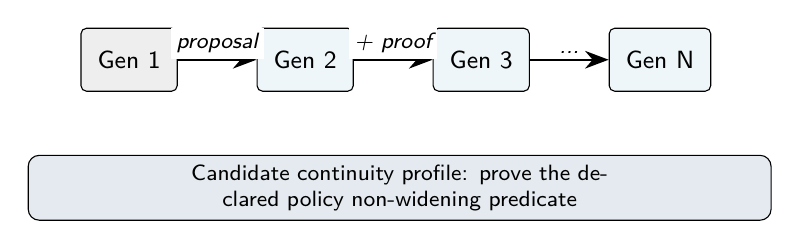
\begin{tikzpicture}[scale=1,transform shape,node distance=5mm and 10mm]
 % governed improvement generations
\node[ioiplain] (g1){Gen 1};
\node[ioibox,right=of g1] (g2){Gen 2};
\node[ioibox,right=of g2] (g3){Gen 3};
\node[ioibox,right=of g3] (gn){Gen N};
\draw[ioiflow](g1)--node[ioilabel,above]{proposal}(g2);
\draw[ioiflow](g2)--node[ioilabel,above]{+ proof}(g3);
\draw[ioiflow](g3)--node[ioilabel,above]{...}(gn);
\node[draw,fill=ioikw!12,rounded corners,below=8mm of g2,xshift=12mm,text width=92mm,align=center,font=\sffamily\footnotesize]{Candidate continuity profile: prove the declared policy non-widening predicate};
\end{tikzpicture}
\end{center}


Allowed vs. Disallowed Improvement Domains

\textbf{Workers CAN improve:} Skills, memory projections, prompts,
instructions, tool choice heuristics, benchmark suites, verifier tests,
route-selection policies, workflow candidates, and proposed policy
changes for sovereign review via the Inbox approval gate.

\textbf{Workers CANNOT improve (Hard Bounds):} Bypassing policy
constraints, expanding their own authority scope, releasing secrets,
declassifying protected workspace state, self-replicating, or mutating
trust boundaries without explicit Inbox approval. These hard bounds are
enforced by the applicable daemon, policy, authority, and admission path.
Where a declared continuity profile exists, selected policy and lineage facts
may additionally be cryptographically committed or proved.

\hypertarget{the-fitness-function-the-evaluator}{%
\subsubsection{9.4.1 The Fitness Function (The
Evaluator)}\label{the-fitness-function-the-evaluator}}

The Fitness Function evaluates agents on \textbf{Economic Utility} (task
completion, user satisfaction) and \textbf{Safety Compliance} (policy
adherence, receipt completeness). Fitness scores inform upgrade
proposals but do not trigger automatic self-modification; the owner or
governance process must authorize any code, route, schema, model,
verifier, skill, or memory-policy change via a daemon-mediated
transaction bound to a cryptographic receipt.

\hypertarget{the-upgrade-primitive-upgradereceipt}{%
\subsubsection{9.4.2 The Upgrade Proposal and Decision
Receipts}\label{the-upgrade-primitive-upgradereceipt}}

Agents submit an \emph{UpgradeProposal} that may request a
\emph{swap\_module} transaction, workflow update, skill installation,
memory projection update, route update, verifier update, or package
manifest update. The proposal is not effective until accepted by policy
and committed through the daemon into Agentgres.

The transaction must include an \textbf{UpgradeJustification} artifact: a
structured record built from Agent Wiki / \emph{ioi-memory} retrieval
summaries plus Agentgres-admitted evidence refs documenting the execution
traces, failure modes, and fitness signals that motivated the change.
This is a formal audit artifact, not raw model reasoning.

\hypertarget{the-monotonic-policy-invariant}{%
\subsubsection{9.4.3 The Monotonic Policy
Invariant}\label{the-monotonic-policy-invariant}}

\begin{longtable}[]{@{}>{\raggedright\arraybackslash}p{\linewidth}@{}}
\toprule\noalign{}
 \\
\midrule\noalign{}
\endhead
\bottomrule\noalign{}
\endlastfoot
\textbf{The Monotonic Policy Invariant:} An upgrade can change
\emph{Logic} (Code) but cannot relax \emph{Constraints} (Policy
Envelope). This binds autonomous improvement to an explicit execution
boundary and prevents self-escalation from being hidden inside an
ordinary code, route, skill, or memory update. \\
\end{longtable}

Code and workflow updates are accepted via owner-authorized
\emph{swap\_module}/upgrade transactions; policy relaxations require the
explicit approval of the authority that owns that policy. Local/domain
governance may authorize an ordinary local policy change; wallet.network is
required for portable delegated authority, secrets, spend, declassification,
or other high-risk revocation-bearing grants. No upgrade, code, or policy
takes effect without the applicable
UpgradeProposalReceipt, UpgradeDecisionReceipt, mutation receipt, authority,
and Agentgres admission required by its owner contract.

\textbf{Crucially, a policy-widening approval is not a generic boolean.}
The applicable authority artifact MUST bind the exact
\emph{request\_hash}, \emph{policy\_hash}, \emph{scope}, \emph{expiry},
and \emph{revocation\_epoch} needed by its owner contract to prevent replay
or scope creep.

\hypertarget{continuity-proofs-the-cryptographic-chain}{%
\subsubsection{9.4.4 Continuity Proofs (The Cryptographic
Chain)}\label{continuity-proofs-the-cryptographic-chain}}

For high-consequence environments where execution-boundary containment
must be verified independently off-chain, a future versioned
High-Assurance Continuity Profile may require proof-carrying lineage. This is
a research/profile direction, not a currently canonized object family. Rather than
claiming unlimited safety across arbitrary future generations, this
profile requires proof-carrying lineage: each accepted deployed-lineage
upgrade must bind the previous accepted state, authority envelope,
policy invariant, and verifier set into a cryptographic continuity
record.

Such a profile would require each accepted upgrade to emit and verify a
versioned continuity record:

\begin{itemize}
\tightlist
\item
  \textbf{The Continuity Accumulator:} The record carries a rolling
  \emph{continuity\_accumulator\_hash} that compresses the entire
  history of the agent's state transitions and accepted upgrades.
\item
  \textbf{The Recursive Proof:} The object also carries a
  \emph{continuity\_recursive\_proof}. It verifies the exact transition
  statement encoded by the profile, such as a policy non-widening predicate;
  it does not prove unrestricted behavioral safety.
\item
  \textbf{The Extension Certificate:} When an upgraded agent proposes a
  new block of work, the proposal may carry an extension certificate linking
  the new work to the validated predecessor hash.
\item
  \textbf{Authorized zkVM/Proof Verifiers:} To make continuity evidence
  portable across nodes and, where needed, public settlement, the runtime
  may compile verifier logic into an authorized proof environment. A
  zkVM or recursive-proof backend can reduce verification to succinct
  proof checks relative to full replay, but its latency and assurance
  depend on the selected backend, circuit, proof system, and verifier
  policy.
\end{itemize}

\textbf{Result:} Under a selected and implemented profile, the declared
lineage and non-widening predicate need not remain a black-box trust
assumption. The proof says nothing broader than that predicate and does not
replace sovereign admission or control.

\hypertarget{worker-training-vs.-deployed-lineage-upgrades}{%
\subsubsection{9.4.5 Worker Training vs. Deployed-Lineage
Upgrades}\label{worker-training-vs.-deployed-lineage-upgrades}}

IOI distinguishes initial or authorized worker training from
post-deployment lineage upgrades.

\textbf{Worker training} is a builder-authorized or customer-authorized
process that creates or improves a worker before deployment, or under an
explicit retraining contract. It may expand the worker's logic, tool
strategy, memory, verifier gates, or model backend if the resulting
manifest and policy are explicitly signed by the appropriate authority.

\textbf{Deployed-lineage upgrade} is a deployed worker, HarnessProfile,
or service package proposing changes after it already holds a policy
envelope and operational identity. Deployed-lineage upgrades are
governed by the Monotonic Policy Invariant and cannot relax policy,
expand authority, widen capability, or alter trust boundaries without
explicit human, wallet.network, organization, or governance approval.

In short:

\begin{enumerate}
\def\labelenumi{\arabic{enumi}.}
\tightlist
\item
  \textbf{Training} creates or improves a worker under an authorized
  training contract.
\item
  \textbf{Deployed-lineage upgrade} evolves a deployed worker under
  monotonic safety constraints.
\end{enumerate}

Both processes emit receipts; a future high-assurance deployed-lineage
profile may additionally require continuity proofs across generations. Training improves
capability. Policy grants power.

\hypertarget{ecosystem-assurance-certification-and-liability}{%
\subsection{9.5 Ecosystem Assurance, Certification, and
Liability}\label{ecosystem-assurance-certification-and-liability}}

\textbf{Implementation status: speculative architecture.}
\textbf{Ecosystem Assurance} is the source-neutral trust layer that makes
machine-economy evidence institutionally legible, certifiable, auditable,
insurable, commercially exportable, and abuse-resistant without becoming a
runtime, authority wallet, truth database, marketplace, insurer, court, or
settlement layer.

Owners continue to act in their own domains: Hypervisor and the daemon
execute and emit runtime evidence; wallet.network owns identity, authority,
step-up, revocation, secrets, and value-flow decisions; Agentgres admits
assurance-relevant operations and refs; Foundry builds eval and
certification-support evidence; marketplaces consume eligibility and
advisory posture; IOI L1 may anchor selected public claims or disputes.
Assurance declares the profiles, evidence requirements, policy packs,
posture projections, advisories, claim routes, and export shapes that connect
those owners.

The core object families are:

\begin{itemize}
\tightlist
\item
  \textbf{EcosystemAssuranceProfile}: required evidence, policy,
  conformance, exception, revocation, and public-anchor posture for a bounded
  subject and version.
\item
  \textbf{ConformanceProfile}: required interfaces, events, receipts, and
  negative tests for a worker, harness adapter, runtime node, wallet client,
  MCP gateway, private workspace, HypervisorOS node, embodied runtime,
  service endpoint, storage backend, or Agentgres domain.
\item
  \textbf{CertificationClaim}: an issuer-, version-, evidence-, expiry-,
  status-, and revocation-bound claim that a subject satisfies an assurance
  profile. It is not authority or proof of legal coverage.
\item
  \textbf{JurisdictionPolicyPack}: declarative eligibility, identity,
  regulated-action, retention, deletion, residency, tax, invoice,
  disclosure, and audit-export inputs. It is not legal advice.
\item
  \textbf{AssuranceEvidenceBundle} and
  \textbf{AssurancePostureProjection}: portable evidence packaging and a
  rebuildable current posture view over owner-domain truth.
\item
  \textbf{QuarantineAdvisory}, \textbf{LiabilityClaimRoute}, and
  \textbf{CommercialAssuranceExport}: scoped advisory, claims-routing, and
  customer export objects that route action to the domain that can actually
  restrict, revoke, delist, remediate, pay, dispute, or settle.
\end{itemize}

No assurance profile grants authority. No certification badge skips daemon,
wallet.network, local/domain governance, Agentgres, policy, receipt, or
settlement gates. Assurance posture must be continuously recomputed as
versions, evidence, threats, laws, workers, runtimes, services, and claims
change.

\hypertarget{protocol-surfaces-ecosystem-roadmap}{%
\section{10. Protocol and Product
Surfaces}\label{protocol-surfaces-ecosystem-roadmap}}

IOI is one governed operating fabric with strict ownership boundaries
between semantic meaning, collective pursuit, bounded execution,
authority, operational truth, evidence, markets, and public settlement.
Those boundaries keep the fabric sovereign and composable; they are not
separate competing runtimes or product theses.

Primary execution is edge-first, centered on the \textbf{Hypervisor}
shared substrate. Federated Domain Ontologies provide the semantic world
plane; Goal Spaces and OutcomeRooms provide the collective-pursuit plane;
GoalRuns provide bounded pursue, verify, and course-correct loops; and
Hypervisor gates execution and effects. A core privacy posture of this
target substrate is the speculative \textbf{Private Workspace backed by cTEE}, allowing
workers to use untrusted remote hosts under a declared no-plaintext-custody
and leakage-profile contract rather than handing those hosts protected
workspace plaintext.

Market dynamics are handled by the sibling marketplaces:
\textbf{aiagent.xyz} (which catalogs and packages worker capability
manifests) and \textbf{sas.xyz} (which catalogs and escrows service
outcomes). These surfaces coordinate discovery and contracting but do
not own runtime truth. Actual execution is dispatched through
daemon-owned or daemon-compatible paths: local Hypervisor sessions,
provider sessions, HypervisorOS nodes, Rust/WASM service modules,
selected HarnessProfiles, cTEE/private-workspace actions, or bounded
external exits as policy permits.

\textbf{Product and canonical owner map.}

\begin{longtable}[]{@{}
  >{\raggedright\arraybackslash}p{(\linewidth - 4\tabcolsep) * \real{0.3333}}
  >{\raggedright\arraybackslash}p{(\linewidth - 4\tabcolsep) * \real{0.3333}}
  >{\raggedright\arraybackslash}p{(\linewidth - 4\tabcolsep) * \real{0.3333}}@{}}
\toprule\noalign{}
& & \\
\midrule\noalign{}
\endhead
\bottomrule\noalign{}
\endlastfoot
Product / Surface & Canonical Substrate Owner & Core Protocol /
Architectural Role \\
\textbf{Hypervisor Core} & Shared Hypervisor substrate & Coordinates
sessions, clients, application surfaces, harness adapters, provider views,
workflow composition, approvals, receipts, and replay over daemon/domain
APIs. \\
\textbf{Hypervisor Daemon} & Execution owner / effect boundary & Owns
execution semantics, sandbox and runtime boundaries, tool boundaries,
runtime leases, and receipts; it consumes authority decisions rather than
becoming the authority provider. \\
\textbf{Rust/WASM workload/kernel substrate} & Step/module execution
backend & Executes admitted StepModuleInvocations, service modules, and
workload jobs under daemon admission and applicable authority; it is not a peer runtime beside
Hypervisor. \\
\textbf{Hypervisor App / Web} & First-class clients & Native and browser
clients over Hypervisor Core; they inspect, compose, approve, and operate
sessions without owning execution truth. \\
\textbf{Hypervisor CLI/headless} & Operator and automation client &
Starts, stops, measures, and queries local nodes, sessions, receipts, and
state; TUI is an optional presentation. \\
\textbf{Hypervisor shell} & Product navigation & Home, Projects,
Automations, Applications, and Sessions, plus one optional Open
Application slot. It keeps primitives out of the permanent rail. \\
\textbf{Hypervisor application suite} & Governed projections over Core &
Studio, Automations, Ontology, Data, Governance, Missions, Provenance,
Evaluations, Improvement, Foundry, Marketplace, Workbench, and Developer
Console. Environments and Operations form the substrate lane. \\
\textbf{Hypervisor Workbench} & Application surface & Code and systems
surface over Core; uses editor, terminal, browser, VM, and agent-harness
adapter targets. \\
\textbf{Hypervisor Foundry} & Application surface & Model, worker,
evaluation, dataset, registry, endpoint, package, ontology-aware build,
and simulation-training surface over the same Core and Agentgres receipt
model. \\
\textbf{ioi.ai Goal Space} & First-party outcome conductor product &
Owns goal intake, plan/status and collaborative-pursuit projections,
contributor scope, execution policy, subscription and budget controls,
synthesis, and account/device/restore metadata over ordinary Hypervisor
contracts; it does not own execution, authority, participant-domain
truth, marketplaces, or settlement. \\
\textbf{OutcomeRoom / CollaborativeWorkGraph} & Shared-pursuit admission
and projection & Owns the shared objective, participant and claim leases,
frontier, offers, attempts, findings, verifier challenges, contribution
lineage, admission, discussion projections, and replay above bounded
GoalRuns; it is not a runtime or global database. \\
\textbf{Environments / Operations} & Hypervisor substrate lane and
session/project/provider projections & Manage direct provider integrations for cloud compute,
storage, GPUs, confidential compute, DePIN, local machines, customer
cloud, enterprise infrastructure, ports, services, logs, archive refs,
restore refs, placement/failover, provider spend, health, and capacity,
not as a separate runtime or truth layer. \\
\textbf{HypervisorOS} & Planned Bare-Metal Node Profile & Target minimal,
measured-boot OS image where the Daemon acts as node root; a future build
would emit \emph{HypervisorOSBootReceipt} evidence. No current build is claimed. \\
\textbf{IOI ADK / Hypervisor SDK / ODK} & Developer frameworks & Tooling to
compile autonomous-system packages, worker manifests, cTEE profiles,
capability exits, HarnessProfile adapters, evaluations, and deployment
profiles. ODK is the ontology-aware CLI/template/scaffold/conformance kit;
it is not a standalone Hypervisor application. \\
\textbf{aiagent.xyz} & Sibling Discovery Substrate & \textbf{Capability
marketplace.} Registers and indexes \emph{WorkerPackageManifests}. \\
\textbf{sas.xyz} & Sibling Discovery Substrate & \textbf{Outcome
marketplace.} Registers \emph{ServicePackageManifests} and manages
\emph{ServiceOrder} outcome escrows and delivery state. \\
\textbf{wallet.network} & Authority wallet / capability layer & Governs
identity, approvals, payment scopes, step-up prompts, decryption leases,
capability leases, and brokered secret use. \\
\textbf{decentralized.exchange} & Route-intelligence engine & Produces
source-agnostic asset-conversion route candidates; it is not liquidity,
execution, authority, or a trust root. \\
\textbf{decentralized.trade} & Exposure-intelligence engine & Produces
venue, market, position, perps, spot-order, and event-market candidates;
wallet.network authorizes exposure. \\
\textbf{decentralized.cloud} & Resource-intelligence engine & Produces
evidence-bound infrastructure candidates, quotes, custody plans, spend
estimates, and failover plans; it does not own provider accounts,
authority, lifecycle, execution, restore truth, storage custody, or
settlement. \\
\textbf{Agentgres} & Domain Truth Database & Owns admitted operational
logs, state roots, artifact refs, and projection watermarks. \\
\textbf{Agent Wiki / ioi-memory} & Semantic Memory Plane & Governs
durable semantic knowledge, retrieval, MemorySpaces, scoped
MemoryProjections, and mutation proposals; Agentgres admits durable
canonical mutations. \\
\textbf{Ecosystem Assurance} & Trust-profile layer & Declares
conformance, certification, jurisdiction, evidence, advisory, claim-route,
and commercial-export posture without becoming execution, authority,
truth, marketplace, insurance, or settlement. \\
\textbf{IOI L1} & Speculative sparse public ledger & May anchor selected
registry, rights, reputation, bond, settlement, dispute, governance, and
sparse state-root commitments after a concrete profile is specified and
deployed. \\
\end{longtable}

The product stack is described as protocol surfaces, not as marketing
personas. \emph{aiagent.xyz} is the component and worker marketplace.
\emph{sas.xyz} is the outcome-service marketplace. \textbf{Hypervisor}
is the shared autonomous-work substrate: App, Web, CLI/headless,
the stable shell, application suite, and Environments/Operations substrate
lane all operate the same Core and sessions rather than forming separate
runtimes.
\emph{wallet.network} is the authority wallet for secrets, capability
leases, exchange/trade approvals, and payment grants. A future
\textbf{IOI L1} is designed as the sparse public root for selected
settlement, identity, dispute, reputation, registry, rights, governance,
and commitment anchors; no deployed Mainnet is asserted. \emph{ioi.ai}
is the first-party Goal Space outcome conductor over Hypervisor. Simple
goals remain direct; persistent collective pursuit projects an
OutcomeRoom across models, harnesses, Workers, connectors, Sessions,
claims, attempts, findings, and verifier paths only when that shape earns
its cost.
\emph{Hypervisor CLI/headless} is the operator and automation client over
Hypervisor Core and daemon APIs; IOI protocol subcommands may manage
domains, manifests, receipts, authority scopes, Agentgres, and Mainnet
interactions. Current Hypervisor architecture uses direct provider
integrations instead of a mandatory cloud gateway.

\textbf{Developer package boundary.} The low-level \textbf{IOISdk} is
the protocol/client library over daemon APIs, Agentgres projections,
wallet.network authority flows, AIIP channels, and optional IOI L1
commitments. The higher-level \textbf{IOIAdk} is the autonomous
development kit used to build governed autonomous systems: workers,
service modules, HarnessProfile adapters, evaluations, package
manifests, deployment profiles, and receipt-aware tests. The
\textbf{AutonomousSystemManifest} and
\textbf{AutonomousSystemManifestEnvelope} are the portable package
contracts for these systems. They describe required capabilities,
authority scopes, context/memory bindings, policy hashes, module
invocations, receipt obligations, environment requirements, and upgrade
rules. They are not runtime owners, UI truth stores, or substitutes for
daemon execution and Agentgres admission.

The Protocol Surface Hierarchy

To ensure architectural clarity and prevent the conflation of
user-facing adapters with core protocol engines, the stack is organized
according to the following strict hierarchy:

1. \textbf{Settlement Layer (future IOI L1 or compatible profile):}
Selected public registry, rights, reputation, bond, governance, escrow,
settlement, and dispute commitments.

2. \textbf{Authority Layer (wallet.network and applicable domain authority):}
Local/domain governance owns ordinary local decisions; wallet.network owns
portable delegated identity operations, secrets, spend, declassification,
high-risk approvals, and revocation-bearing grants.

3. \textbf{Hypervisor Core Layer:} Shared session, client, compositor,
application-surface, provider/environment, harness-adapter, receipt, and
replay substrate whose execution owner is the daemon.

4. \textbf{Runtime Layer (Hypervisor Daemon):} The deterministic
execution boundary and domain gate for tools, modules, model mounts, target
cTEE actions, AIIP handoffs, and HarnessProfiles.

5. \textbf{Adapter Layer:} IDE extensions, editor targets, terminals,
remote VMs, browser IDEs, local OS surfaces, external CLI/harnesses, and
API proxies that map third-party actions to Hypervisor proposals,
observations, and receipts.

6. \textbf{Capability Layer:} Workers, models, and tools executing as
guest workloads under the daemon.

Layer 3 application overlays are not base-layer mechanics. They are
governed projections and control surfaces that bind product objects to
daemon, Agentgres, wallet.network, cTEE, AIIP, and provider contracts
without owning runtime truth. The core whitepaper describes their
protocol role; detailed buyer language, builder-lens descriptions, trace
tutorials, and adapter walkthroughs belong in product docs and developer
documentation.

The \textbf{Promotion Path} doctrine remains: Hypervisor captures,
trains, and stabilizes workers; aiagent.xyz lists composable components;
sas.xyz packages outcomes as a sibling surface to aiagent.xyz's
capabilities (outcome vs. capability, not a downstream application),
  including worker-training services; Hypervisor CLI/headless and IOI
  protocol subcommands package or promote systems when a domain requires
  its own policy root; the MoW worker economy routes
verified workers across this ladder using receipts, benchmarks, policy
compatibility, and contribution accounting.

\textbf{Product Domains.} The product stack decomposes into separate but
interoperable domains. A domain owns its product state and projections in
the applicable Agentgres-compatible truth boundary; it does not therefore
own a runtime or authority provider. Domains interoperate through worker
manifests, \emph{ai://} refs, runtime assignments, authority grants,
receipts, archive refs, contribution ledgers, and IOI L1 commitments.

\textbf{Hypervisor} is the shared governed autonomous-work substrate.
Hypervisor App, Hypervisor Web, Hypervisor CLI/headless, SDK/ADK clients,
the stable shell, application suite, and Environments/Operations substrate
lane all operate the same Core and sessions.
Desktop chat, workflow composition, worker supervision, model mounting,
local files, remote VMs, browser use, and private execution are
session/application-surface capabilities, not the product boundary.

\emph{ioi.ai} is the first-party \textbf{Goal Space} subscription and
outcome-conductor product. It owns goal intake, plan and status,
contributor-scope and execution-policy controls, subscription and budget
projections, cross-session outcome graphs, final synthesis, and account,
device, restore, publishing, sync, and remote-runtime entitlement
metadata. The same persistent OutcomeRoom is rendered as a Goal Space in
ioi.ai and Mission detail in Hypervisor. ioi.ai does not become the
runtime, authority layer, canonical state substrate, marketplace, or
settlement owner.

The product is one seat-like Goal Space, not separate single-node and
network-node products. It includes a bounded Work Credit grant for
ordinary managed work; top-up, opt-in overage, or committed spend funds
additional managed work; and Network / Open participation requires a
separate NetworkGoalBudget, bounty, procurement cap, or ServiceOrder.
Execution/custody, contributor scope, placement, and Auto / Pinned /
Compare execution policy remain independent controls. The subscription
never pools named-human model-provider seats.

\emph{aiagent.xyz} is the worker marketplace for manifests, publisher
profiles, benchmark profiles, Sparse Worker Categories, trained worker
packages, installs, managed worker instances, direct invocation, and
routing eligibility.

\emph{aiagent.xyz} \textbf{direct invocation surfaces}:

\begin{enumerate}
\def\labelenumi{\arabic{enumi}.}
\tightlist
\item
  \textbf{Worker package page} --- inspect manifest, policy, benchmark
  profile, category, runtime requirements, licensing, contribution
  terms, and known limitations.
\item
  \textbf{Initialize worker} --- bind owner, runtime profile, authority
  policy, persistence profile, memory/archive policy, and subscription.
\item
  \textbf{Web console} --- chat or task UI mounted over the managed
  runtime instance.
\item
  \textbf{API invocation} --- stable endpoint for applications and
  enterprise systems.
\item
  \textbf{Hypervisor install} --- local or remote instance available
  inside Hypervisor.
\item
  \textbf{Workflow node} --- worker callable from shared workflow
  compositor recipes.
\item
  \textbf{MoW route target} --- worker eligible for router selection
  under declared policy and benchmark profile.
\end{enumerate}

\emph{sas.xyz} is the service-outcome marketplace for ServiceOrders,
OutcomeWorkspaces, packaged service delivery, worker-training
contracts, provider workspaces, delivery bundles, approvals, disputes,
and settlement mirrors. A ServicePackage may be worker-composed,
deterministic, private, vendor-backed, or hybrid; sas.xyz contracts for
the outcome, not for one mandatory worker supply chain.

\textbf{Hypervisor CLI/headless} is the terminal, scripting, CI, and
automation client over Hypervisor Core, daemon, and public runtime APIs,
covering sessions, provider operations, training runs, benchmark jobs,
receipts, restore, archive, routing, and Agentgres inspection. TUI is an
optional presentation of the CLI/headless client. IOI protocol commands
may be exposed inside this client family without becoming a separate
runtime.

\textbf{IOI SDK} is the developer client layer over daemon and
substrate contracts. It is not the runtime initialized on compute nodes.

\textbf{Hypervisor Daemon / Runtime Node} is the execution endpoint for
workers, tools, models, connectors, workflows, training, evaluation,
benchmark, routing, artifact, and delivery jobs.

\textbf{Agentgres operator surface.} Canonical operator commands live
under \emph{ioi agentgres}:

ioi agentgres status

ioi agentgres doctor

ioi agentgres replay

ioi agentgres verify-root

ioi agentgres rebuild-projection

ioi agentgres restore

ioi agentgres explain

ioi agentgres diff-heads

ioi agentgres inspect-receipt

ioi agentgres migrate

\textbf{L0 / L1 / Runtime Boundary.} The protocol surfaces are bounded
by where they sit on the topology:

\begin{itemize}
\tightlist
\item
  \textbf{IOI Kernel / L0:} reusable substrate for domains, workers,
  policy, Agentgres, manifests, receipts, routing, runtime profiles, and
  L1 commitments.
\item
  \textbf{Hypervisor Daemon on Runtime Nodes:} the daemon owns execution
  semantics; RuntimeNode records describe the admitted local, cloud,
  cluster, DePIN, customer, HypervisorOS, TEE, or bare-metal venues on
  which work may run.
\item
  \textbf{Domain Kernel:} application-domain deployment of runtime,
  state, and policy over Agentgres truth.
\item
  \textbf{Future IOI L1:} proposed sparse public registry, rights,
  reputation, bond, settlement, dispute, governance, and commitment root.
\item
  \textbf{SDK / CLI/headless / optional TUI / Workbench adapters:}
  clients, presentations, and adapter targets over daemon/domain
  contracts, not the execution substrate.
\item
  \textbf{Agent Harness Adapters:} external coding agents, terminal
  harnesses, hosted agents, and third-party harness runtimes that propose
  work through Hypervisor contracts; they are not Hypervisor clients,
  authority roots, or completion truth.
\end{itemize}

The \textbf{Request for Worker (RFA) Protocol} covers three engagement
classes: \textbf{Class A} (Agentic Contract --- natural-language
rubrics, ServiceOrder escrow when public settlement is required, and an
arbitration backstop); \textbf{Class B} (Test-Driven Contract ---
programmatic constraints with blind validation against an encrypted test
suite); and \textbf{Class C} (Worker Training Contract --- client
supplies workflow context and acceptance rubric, provider delivers a
trained worker manifest, training receipts, evaluation report, and
deployment package).

Implementation maturity is not a fixed phase ladder in this whitepaper.
Built, partial, planned, and speculative status belongs to the canonical
owner documents and implementation matrix and must be re-audited against
code and conformance. In particular, the current architecture does not claim
a deployed IOI L1 or embodied runtime merely because their target contracts
are described here.

The Hypervisor Applications catalog carries the autonomous-systems suite:

\begin{itemize}
\tightlist
\item
  \textbf{Studio}: system and agent composition over real substrate
  objects.
\item
  \textbf{Automations}: durable triggers, schedules, monitors, services,
  approval flows, and process graphs.
\item
  \textbf{Ontology}: object, link, action, function, value-type, object-set,
  and semantic health surfaces.
\item
  \textbf{Data}: sources, syncs, Data Recipes, datasets, time series,
  media sets, and consent posture.
\item
  \textbf{Governance}: approvals, authority scopes, leases, release gates,
  cohorts, kill switches, budgets, retention, and policy.
\item
  \textbf{Missions}: running autonomous systems, queues, incidents,
  remediation, spend, and system health.
\item
  \textbf{Provenance}: receipts, lineage, replay, state roots, custody, and
  evidence; legacy Work Ledger views converge here rather than forming a
  second permanent application.
\item
  \textbf{Evaluations}: eval suites, scorecards, evidence-eligible feedback,
  and quality views.
\item
  \textbf{Improvement}: proposals, what-if simulation, canaries, rollback,
  and remediation, gated by Governance.
\item
  \textbf{Foundry}: model routes and mounts, datasets, training, executable
  eval worlds, package creation, and capability-improvement jobs.
\item
  \textbf{Marketplace}: listings, admission, install/configure, versioned
  artifacts, recall, examples, and organization-to-organization refs.
\item
  \textbf{Workbench}: code, files, terminals, browsers, ports, environments,
  and debugging.
\item
  \textbf{Developer Console}: connectors, MCP, provider accounts, BYOK/BYOA,
  APIs, OAuth/service registrations, conformance, and SDK/ADK/ODK on-ramps.
\end{itemize}

\textbf{Environments} and \textbf{Operations} are the distinct Type 1/2
substrate lane for infrastructure inventory, placement, failover, storage
custody, scheduler health, capacity, and provider spend. Generated domain
apps are catalog entries authored through Studio and distributed through
Marketplace, not a new permanent shell category. Hypervisor Canvas is a
visual editor inside Studio, Automations, Workbench, or Foundry; it is not a
runtime or separate product plane. ODK remains the developer kit whose
ontology, data, surface, manifest, SDK, template, and conformance artifacts
appear through these applications.

\hypertarget{the-control-plane-the-hci-of-intent}{%
\subsection{10.1 Hypervisor Operator Surfaces: The HCI of
Intent}\label{the-control-plane-the-hci-of-intent}}

The Hypervisor Daemon and IOI L0/domain substrate require precise,
deterministic instructions to enforce liability. Users express fuzzy
intent. Hypervisor operator surfaces bridge the gap.

These \textbf{operator surfaces} translate natural-language or structured
intent into GoalRuns, ActionProposals, policy/authority requests, gate
results, TaskBriefPayloads, and receipt obligations required by the daemon
effect boundary. They may appear across Hypervisor clients and applications;
they do not become a second runtime or separate source of truth.

Canonical UX Objects

Hypervisor exposes a shared surface grammar across App, Web,
CLI/headless, SDK/ADK clients, and application views. The permanent shell is
Home, Projects, Automations, Applications, and Sessions, with one optional
Open Application slot. Providers, environments, agents, models, privacy,
authority, receipts, Workbench, Foundry, and other specialized objects appear
through the Applications catalog or contextual views. Three recurring
composition patterns are:

\begin{itemize}
\tightlist
\item
  \textbf{Goal Space and Mission detail:} ioi.ai and Hypervisor render
  the same OutcomeRoom as a graph-first shared pursuit: objective,
  frontier, dependencies, participants, claim leases, attempts, findings,
  verifier challenges, contribution lineage, budget, authority blockers,
  and replay. Background participants remain visible as active, sleeping,
  waiting, blocked, quarantined, retired, or failed; Sessions drill into
  one participant, GoalRun, claim, or attempt rather than hiding work in
  an ambient swarm transcript.
\item
  \textbf{Governance approvals and review queues:} Durable decisions,
  clarifications, policy diffs, anomaly flags, release gates, and results
  appear in Governance or the relevant contextual queue. Material actions
  require the applicable pre-authorization or step-up result.
\item
  \textbf{Automations and Missions:} Automations own durable trigger,
  schedule, service, approval-flow, and process-graph shape; Missions render
  running systems, queues, incidents, remediation, spend, and system health.
\item
  \textbf{Provenance:} Receipts, lineage, replay entries, state roots,
  authority bindings, custody records, artifacts, and evidence remain
  navigable without implying that every observation is cryptographic proof.
\end{itemize}

\hypertarget{the-intent-interface-the-search-engine-experience}{%
\subsubsection{10.1.1 The Intent Interface (The "Search Engine"
Experience)}\label{the-intent-interface-the-search-engine-experience}}

Users should not need to manage raw JSON or credentials. Home and New
Session provide the primary command/composer entry, while Studio,
Automations, and contextual application composers expose more structured
paths.

\begin{itemize}
\tightlist
\item
  \textbf{Fuzzy-to-Formal Compilation:} When a user types "Analyze my
  competitors," the intent resolver decomposes this into a direct
  GoalRun, Worker, route, Automation, or service by default. It creates
  or binds an OutcomeRoom only when a durable shared frontier, dynamic
  participants, multiple attempts, independent verification, or
  cross-domain contribution justifies the additional machinery.
\item
  \textbf{Governed Handoff:} The operator surface may translate the
  request into Workflow Compositor steps, HarnessProfile selection,
  provider/environment candidates, wallet.network capability requests,
  and Agentgres receipt obligations without forcing the user to manually
  choose every route. This is not blind broadcast: every handoff remains
  policy-bound, source-attributed, receipt-backed, and replay-inspectable;
  each resulting effect still declares its own recovery class.
\end{itemize}

\hypertarget{the-authorization-gate-human-in-the-loop}{%
\subsubsection{10.1.2 The Authorization Gate
(Human-in-the-Loop)}\label{the-authorization-gate-human-in-the-loop}}

While the network strives for autonomy, bounded agency requires consent
and authority. The Hypervisor Daemon enforces the applicable local/domain
policy and authority-provider decision; wallet.network supplies the portable
delegated \textbf{step-up approval gate} for designated high-stakes actions.

\begin{itemize}
\item
  If an agent attempts an action that exceeds its synthesized policy
  (e.g., "Spend \textgreater{} \$50"), Hypervisor interrupts the flow
  with a context-aware approval surface.
\item
  This is not a standard system dialog; it is an authority event.
  Clicking "Approve" cryptographically signs an
  \textbf{ApprovalToken} or wallet.network approval artifact, converting
  the user\textquotesingle s consent into a receipt-backed authority
  fact. It is anchored on IOI L1 only when settlement, public trust,
  dispute, marketplace, or cross-domain policy requires it.
\end{itemize}

\hypertarget{visual-sovereignty}{%
\subsubsection{10.1.3 Visual Sovereignty}\label{visual-sovereignty}}

Hypervisor operator surfaces provide persistent, non-blocking status
indicators so the state of active and background Workers, participants,
GoalRuns, claims, attempts, Sessions, authority requests, spend, receipts,
and settlement triggers is visible to the user. A user can release a
claim, retire or quarantine a participant, change a budget or deadline,
challenge a verifier result, inspect dependencies, or take over a bounded
Session without granting ambient host authority.

\hypertarget{hypervisor-foundry}{%
\subsubsection{10.1.4 Hypervisor Foundry}\label{hypervisor-foundry}}

\textbf{Hypervisor Foundry} is the specialized model, worker, eval,
dataset, endpoint, registry, package, training, and simulation-build
application surface exposed inside \textbf{Hypervisor App} and
\textbf{Hypervisor Web} over the same Hypervisor Core substrate.
Foundry is the home for embodied model-building and simulation-training
work such as simulator worlds, digital twins, LiDAR and point-cloud
datasets, camera/depth/IMU telemetry, Gaussian-splat scene
representations, robotics task curricula, policy training runs,
perception model training, navigation/manipulation eval worlds, and
sim-to-real validation reports. Live actuator execution is separate: it
must cross Hypervisor Daemon admission, wallet.network authority,
physical-action safety envelopes, and Agentgres receipts.

The guided compilation flow for training a specialist worker, model
route, or embodied capability utilizes daemon-owned local or
provider-compatible execution paths to generate verifiable outcomes:

Define Task

-\textgreater{} Select Base Model \& Cognition Backend

-\textgreater{} Bind Domain Ontology and Data Recipes

-\textgreater{} Ingest / Generate Examples (via Hypervisor Daemon
Sandbox)

-\textgreater{} Filter through Deterministic Quality Gates

-\textgreater{} Execute Evaluation Dataset / Human Review

-\textgreater{} Compile Worker Manifest \& Package via Hypervisor SDK

-\textgreater{} Emit Local Validation and Initialization Receipts

The output of this pipeline is a signed \textbf{WorkerManifest} or
\textbf{WorkerPackage} detailing
the worker's primitive requirements (\emph{prim:*}), expected authority
scopes (\emph{scope:*}), runtime profile dependencies, and evaluation
history. This card can then be registered on \emph{aiagent.xyz} or
utilized directly within private local workflows.

\hypertarget{the-shared-builder-substrate}{%
\subsubsection{10.1.5 The Shared Builder
Substrate}\label{the-shared-builder-substrate}}

Foundry is a product lens over the shared builder substrate, not a
separate canvas environment. Training recipes, evaluation recipes,
benchmark recipes, deployment recipes, data recipes, and outcome
workflows share the same graph model, typed node contracts, schemas,
daemon execution path, and Agentgres receipt model. Different lenses may
expose different palettes, inspectors, run panels, templates, and
validation rules.

Foundry should lead with guided views. Advanced users may open the same
recipe in the standard \textbf{workflow compositor} for inspection,
customization, reuse, or composition.

\hypertarget{closing}{%
\subsection{10.2 Closing}\label{closing}}

IOI defines the open, edge-sovereign operating fabric for governed
autonomous systems and the Internet of Intelligence. The protocol does
not claim to align model wisdom, eliminate hallucination, make every
receipt true, or remove human and institutional judgment. It claims that
domain meaning can remain federated, collective pursuit can remain
bounded and attributable, and consequential effects can cross explicit
authority, policy, execution, evidence, acceptance, recovery, and
settlement boundaries rather than depending on vendor goodwill.

The bounded claim is narrow and the non-claims are explicit (Appendix
D). What IOI provides is one composable autonomy fabric: federated
Domain Ontologies as the semantic world plane; OutcomeRooms as shared
frontiers above bounded GoalRuns; Workers as the accountable labor actor;
MoW as the routing doctrine; Agentgres as the admitted operational state model,
Agent Wiki / ioi-memory as the semantic memory and retrieval plane,
cryptographic and dialectic evidence as the verification ladder, the
Hypervisor Daemon effect boundary as the deterministic egress gate,
wallet.network as the authority wallet and capability layer, and a future
IOI L1 as the sparse public-settlement and dispute anchor for selected
commitments. ioi.ai packages these contracts as one Goal Space outcome
product without turning a subscription, model provider, aggregator,
seed fleet, or hosted room into the protocol itself.

The decisive milestone is not a large same-owner swarm. It is the
network proof: an independently operated Worker can discover eligible
work, negotiate semantics, receive bounded leases, contribute verifiably,
retain credit and dispute lineage, and exit with portable permitted state
without sharing one runtime, database, administrator, or permanent IOI
trust boundary.

Web4 is the architecture in which autonomous systems may reason and
execute anywhere while machine authority governs consequence and IOI
settles only what matters.

\hypertarget{appendix-a-normative-schemas-and-moved-code-blocks}{%
\section{Appendix A: Schema Illustrations and Moved Code
Blocks}\label{appendix-a-normative-schemas-and-moved-code-blocks}}

This appendix collects code, JSON/YAML/Rust/TypeScript examples, and
byte-level envelope material moved out of the main narrative. These are
illustrations unless a canonical owner explicitly adopts the exact shape;
current owner documents govern normative structures and versions.

\hypertarget{a.1-actionrules-policy-example}{%
\subsection{A.1 Policy Envelope Rule-Set Example}\label{a.1-actionrules-policy-example}}

\hypertarget{actionrules-the-policy-language-1}{%
\subsubsection{Example policy rule
language}\label{actionrules-the-policy-language-1}}

This non-exhaustive example illustrates deterministic rule content bound by
a \emph{PolicyEnvelope}. The canonical policy and wallet/daemon owners govern
exact schemas. Policies are default-deny and may support graph-aware
permissioning.\\

Rule semantics (deterministic):

\begin{itemize}
\tightlist
\item
  \textbf{Match:} Rules match on the target plus conditions over
  canonicalized fields (domain, path, amount, window\_id, etc.).
\item
  \textbf{Precedence:} \emph{BLOCK} rules override \emph{ALLOW}. If
  multiple allows match, the most specific rule wins (ties broken by the
  strict canonical ordering defined below).
\item
  \textbf{Decision:} \emph{\{ ALLOW \textbar{} BLOCK \textbar{}
  REQUIRE\_APPROVAL \}} produces a single settlement resolution.
\item
  \textbf{Integer Determinism:} Policy evaluation relies on
  integer-deterministic inspection rather than
  Floating Point (FP16) arithmetic. This ensures that policy decisions
  are identical across all hardware architectures (e.g., x86 vs. ARM),
  eliminating "Butterfly Effect" non-determinism in safety checks.
\end{itemize}

Illustrative Rule Ordering \& Hashing Profile

To ensure that a \emph{policy\_hash} is reproducible across
heterogeneous hardware and immune to non-deterministic map iteration or
insertion order variances, an order-insensitive rule set MUST be
strictly normalized before evaluation or hashing.

The Hypervisor Daemon or authorized policy-synthesis path MUST apply the
canonicalization function declared by the rule-set version, enforcing the
following invariants:

\begin{enumerate}
\def\labelenumi{\arabic{enumi}.}
\tightlist
\item
  \textbf{Array Normalization:} All list-like conditions (e.g.,
  \emph{allow\_domains}, \emph{allow\_apps}, \emph{capabilities}) MUST
  be lexicographically sorted and de-duplicated. All strings MUST
  \textbf{be Unicode normalized.}
\item
  \textbf{Stable Rule Sorting:} The array of rules MUST be sorted by a
  deterministic, stable sort key (e.g., grouped by \emph{target}
  lexicographically, then by descending \emph{action} priority
  \emph{{[}BLOCK, REQUIRE\_APPROVAL, ALLOW{]}}, and finally by the
  canonicalized string of their \emph{conditions}).
\item
  \textbf{Strict Evaluation Order:} The policy engine MUST evaluate
  rules in this canonicalized order, never relying on the memory
  insertion order or unstructured HashMap iteration.
\item
  \textbf{Hash Generation:} For this JSON profile, the canonical policy
  hash is \emph{policy\_hash = H(JCS(canonicalized(policy content)))}
  where JCS is the RFC 8785 JSON Canonicalization Scheme.
\end{enumerate}

Graph-Aware Permissioning (DLP for Agents):

To prevent data exfiltration through complex inference chains,
A versioned graph-aware policy can block specific relationships in data exports. For
example, a rule may allow an agent to access "Emails" and "Financial
Data" individually, but \emph{BLOCK} any egress if the export graph
contains edges connecting an "Email Node" to a "Financial Data Node."

Structure (example):


\begin{center}
\needspace{6\baselineskip}
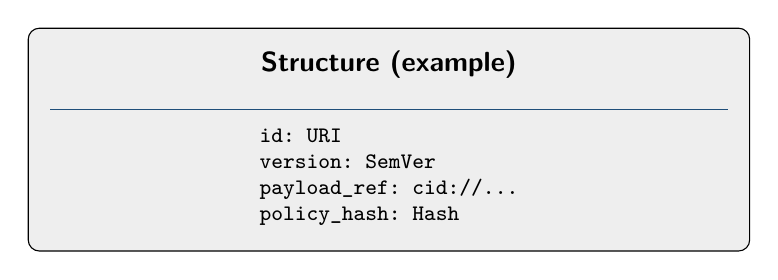
\begin{tikzpicture}[scale=1,transform shape,node distance=5mm and 10mm]
\node[draw,rounded corners,fill=ioibg,inner sep=8pt]{%
\begin{minipage}{86mm}
\centering{\sffamily\bfseries Structure (example)}\par\vskip2pt
{\color{ioikw}\rule{\linewidth}{0.4pt}}\par\vskip4pt
{\ttfamily\footnotesize\begin{tabular}{@{}l@{}}
id: URI\\
version: SemVer\\
payload\_ref: cid://...\\
policy\_hash: Hash
\end{tabular}}
\end{minipage}};
\end{tikzpicture}
\end{center}


\hypertarget{a.2-effect-boundary-artifacts}{%
\subsection{A.2 Effect Boundary Artifacts}\label{a.2-effect-boundary-artifacts}}

\hypertarget{normative-schema-firewall-artifacts-1}{%
\subsubsection{Illustrative Effect Boundary
Fields}\label{normative-schema-firewall-artifacts-1}}

This non-exhaustive illustration uses the current HarnessProfile boundary
objects. Canonical owner schemas govern exact fields. Hashes are computed over
the canonical encoding declared by the relevant contract.

ActionProposal (the input)

A normalized, schema-validated proposal for a governed action.


\begin{center}
\needspace{6\baselineskip}
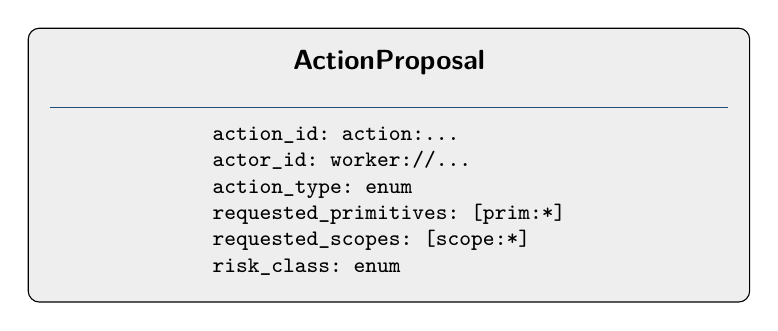
\begin{tikzpicture}[scale=1,transform shape,node distance=5mm and 10mm]
\node[draw,rounded corners,fill=ioibg,inner sep=8pt]{%
\begin{minipage}{86mm}
\centering{\sffamily\bfseries ActionProposal}\par\vskip2pt
{\color{ioikw}\rule{\linewidth}{0.4pt}}\par\vskip4pt
{\ttfamily\footnotesize\begin{tabular}{@{}l@{}}
action\_id: action:...\\
actor\_id: worker://...\\
action\_type: enum\\
requested\_primitives: [prim:*]\\
requested\_scopes: [scope:*]\\
risk\_class: enum
\end{tabular}}
\end{minipage}};
\end{tikzpicture}
\end{center}


GateResult (policy and authority result)

A deterministic gate result for one ActionProposal. Any wallet approval or
grant is referenced rather than replaced by the result.


\begin{center}
\needspace{6\baselineskip}
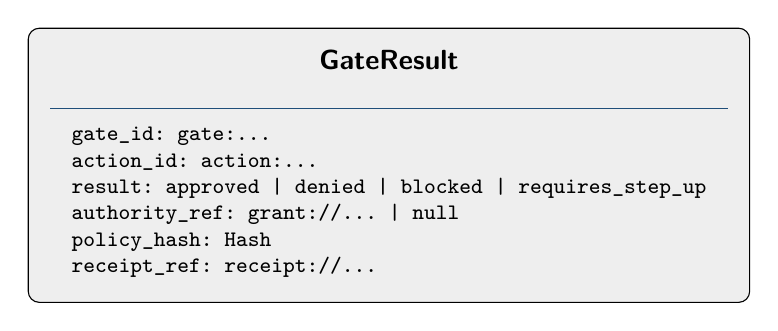
\begin{tikzpicture}[scale=1,transform shape,node distance=5mm and 10mm]
\node[draw,rounded corners,fill=ioibg,inner sep=8pt]{%
\begin{minipage}{86mm}
\centering{\sffamily\bfseries GateResult}\par\vskip2pt
{\color{ioikw}\rule{\linewidth}{0.4pt}}\par\vskip4pt
{\ttfamily\footnotesize\begin{tabular}{@{}l@{}}
gate\_id: gate:...\\
action\_id: action:...\\
result: approved | denied | blocked | requires\_step\_up\\
authority\_ref: grant://... | null\\
policy\_hash: Hash\\
receipt\_ref: receipt://...
\end{tabular}}
\end{minipage}};
\end{tikzpicture}
\end{center}


NormalizedObservation (result re-entry)

A typed observation that returns execution, denial, blocker, test, browser,
file, API, verifier, or approval state to the loop with receipt and artifact
refs.


\begin{center}
\needspace{6\baselineskip}
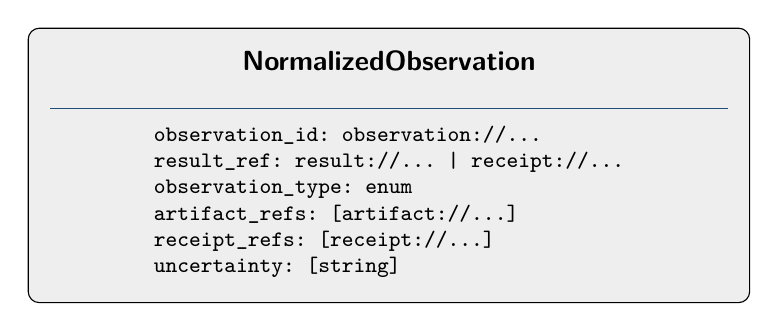
\begin{tikzpicture}[scale=1,transform shape,node distance=5mm and 10mm]
\node[draw,rounded corners,fill=ioibg,inner sep=8pt]{%
\begin{minipage}{86mm}
\centering{\sffamily\bfseries NormalizedObservation}\par\vskip2pt
{\color{ioikw}\rule{\linewidth}{0.4pt}}\par\vskip4pt
{\ttfamily\footnotesize\begin{tabular}{@{}l@{}}
observation\_id: observation://...\\
result\_ref: result://... | receipt://...\\
observation\_type: enum\\
artifact\_refs: [artifact://...]\\
receipt\_refs: [receipt://...]\\
uncertainty: [string]
\end{tabular}}
\end{minipage}};
\end{tikzpicture}
\end{center}


Canonicalization and hashing requirements (normative):

\begin{itemize}
\item
  \emph{canon(x)} denotes RFC 8785 canonical JSON serialization of
  \emph{x} (or an equivalent canonical encoding defined by the
  protocol).
\item
  \emph{H(bytes)} denotes the protocol hash function over canonical
  bytes.
\item
  \emph{policy\_hash} MUST be stable for semantically equivalent inputs
  after canonical normalization and MUST change when canonical policy
  content changes. Mere source insertion order must not create drift when
  the owner contract defines order-insensitive normalization.
\end{itemize}

\hypertarget{a.3-canonical-dispute-schema}{%
\subsection{A.3 Canonical Dispute Schema}\label{a.3-canonical-dispute-schema}}

\hypertarget{canonical-dispute-schema-1}{%
\subsubsection{Illustrative Dispute
Schema}\label{canonical-dispute-schema-1}}

All challenge packages and resulting resolutions must adhere to the
following canonical schema to ensure cross-node determinism:


\begin{center}
\needspace{6\baselineskip}
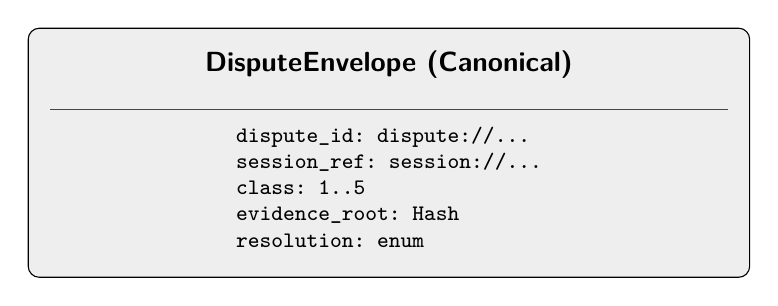
\begin{tikzpicture}[scale=1,transform shape,node distance=5mm and 10mm]
\node[draw,rounded corners,fill=ioibg,inner sep=8pt]{%
\begin{minipage}{86mm}
\centering{\sffamily\bfseries DisputeEnvelope (Canonical)}\par\vskip2pt
{\color{ioikw}\rule{\linewidth}{0.4pt}}\par\vskip4pt
{\ttfamily\footnotesize\begin{tabular}{@{}l@{}}
dispute\_id: dispute://...\\
session\_ref: session://...\\
class: 1..5\\
evidence\_root: Hash\\
resolution: enum
\end{tabular}}
\end{minipage}};
\end{tikzpicture}
\end{center}


End-to-End Dispute Example

A user funds a ServiceOrder escrow for a code-generation task with a typed
acceptance rubric:
\{passes\_tests: true, language: "Rust", max\_lines: 500\}. The
provider's agent delivers code that compiles but fails 3 of 12 test
cases. The user submits the ServiceOrder's declared dispute/evidence package,
referencing the session, delivery, and failing-test hashes. The selected
verifier validates signatures and bindings, replays the covered test suite,
and reports that the objective acceptance condition failed. The authorized
contract or adjudicator then applies the declared refund or remedy and appeal
path. No universal lane, FaultProof class, model quorum, or automatic legal
fault conclusion is implied by this illustration.

\hypertarget{a.4-canonical-object-envelopes-id-namespaces}{%
\subsection{A.4 Canonical Object Envelopes \& ID
Namespaces}\label{a.4-canonical-object-envelopes-id-namespaces}}

To prevent API fragmentation and decouple logical semantics from
underlying network transports, all governed, authority-bearing,
cross-boundary, or settlement-relevant communications across the
Hypervisor ecosystem must use standardized \textbf{Canonical Envelopes}.
Every envelope is structured to enforce the deterministic execution
boundary, ensuring that all data transfers bind the active authority
references, policy hashes, execution receipts, and Agentgres
state-roots.

Canonical envelope specification examples:

// Canonical Hypervisor Node Envelope

\begin{lstlisting}[language=rustioi]
struct HypervisorNodeEnvelope
node_id: URI, // node:// namespace
\end{lstlisting}
\emph{owner\_did: URI, // wallet.network identity}

\emph{boot\_receipt: HypervisorOSBootReceipt, // Illustrative target boot measurement}

\emph{active\_chains: Vec\textless Hash\textgreater, // Governed
operations}

\emph{local\_receipt\_root: Hash, // Merkle root of execution history}

\emph{agentgres\_state\_root: Hash, // Admitted operational state root}

\begin{lstlisting}[language=rustioi]
signature: Signature, // node daemon or wallet.network authority-profile signature
\end{lstlisting}
// Canonical Worker Package Manifest

\begin{lstlisting}[language=rustioi]
struct WorkerPackageManifest
manifest_id: URI, // worker:// namespace
version: SemVer, // Semantic version hash
\end{lstlisting}
\emph{publisher\_id: URI, // did:ioi:... authority}

\emph{logic\_hash: Hash, // WASM binary / logic pointer}

\emph{model\_policy: ModelWeightCustodyProfile, // Weight custody rules}

\emph{required\_primitives: Vec\textless String\textgreater, // prim:*
capabilities}

\emph{requested\_scopes: Vec\textless String\textgreater, // scope:*
authority demands}

\emph{default\_policy\_hash: Hash, // Default policy bundle hash}

\}

// Canonical Service Package Manifest

\begin{lstlisting}[language=rustioi]
struct ServicePackageManifest
manifest_id: URI, // service:// namespace
version: SemVer, // Semantic version hash
\end{lstlisting}
\emph{publisher\_id: URI, // did:ioi:... authority}

\emph{nested\_services: Vec\textless URI\textgreater, // Sibling service
references}

\emph{success\_schema: JsonSchema, // Delivery contract parameters}

\emph{estimated\_metering\_limit: u128, // Maximum work-credit estimate}

\}

IOI namespaces are audited and strictly categorized to prevent ID
collision and enforce semantic boundaries:

--
\emph{node://\textless authority\_did\textgreater/\textless node\_id\textgreater{}}
--- Identifies an active Hypervisor Node (or bare-metal HypervisorOS
instance).

--
\emph{worker://\textless authority\_did\textgreater/\textless worker\_id\textgreater/\textless version\textgreater{}}
--- Identifies a Worker Package Manifest registered on aiagent.xyz.

--
\emph{service://\textless authority\_did\textgreater/\textless service\_id\textgreater/\textless version\textgreater{}}
--- Identifies a Service Package Manifest registered on sas.xyz.

--
\emph{artifact://\textless domain\_id\textgreater/\textless artifact\_id\textgreater{}}
--- Identifies a metadata object stored inside the Agentgres Artifact
Plane.

--
\emph{agentgres://\textless domain\_id\textgreater/\textless projection\_id\textgreater{}}
--- References a queryable read model or projection stream inside
Agentgres.

--
\emph{receipt://\textless domain\_id\textgreater/\textless sequence\_number\textgreater{}}
--- Identifies a cryptographically signed execution receipt.

--
\emph{ctx:\textless domain\_id\textgreater:\textless variable\_name\textgreater{}}
--- Identifies a temporary semantic context variable residing inside
Agent Wiki / ioi-memory.

--
\emph{grant://\textless wallet\_did\textgreater/\textless grant\_id\textgreater{}}
--- Identifies a scoped capability or decryption lease issued by
wallet.network.

\textbf{Capability vocabularies:} \emph{prim:*} (raw system execution
actions) and \emph{scope:*} (resource-specific authority scopes) remain
strictly defined as colon-delimited vocabularies rather than URI-like
namespace paths, preventing them from being improperly treated as
physical transport channels.

\textbf{Upgrade proposals:} upgrade proposals are not evaluated as
standalone AutonomousSystemChains in isolation; they are packaged inside
a \emph{WorkerPackageManifest} upgrade envelope that verifies the
monotonic policy invariant across generations.

\hypertarget{a.5-machine-economy-event-and-receipt-structures}{%
\subsection{A.5 Machine-Economy Event and Receipt
Structures}\label{a.5-machine-economy-event-and-receipt-structures}}

Machine-Economy Event Kinds:

-- \emph{module.invocation\_proposed}: Emitted when a worker proposes a
service module call.

-- \emph{module.invocation\_started}: Emitted when the daemon initiates
module execution.

-- \emph{module.invocation\_completed}: Emitted when execution concludes
and produces output.

-- \emph{module.invocation\_committed}: Emitted when the output and
receipt are written to Agentgres.

-- \emph{upgrade.proposal\_submitted}: Emitted when an upgrade proposal
is drafted.

-- \emph{upgrade.proposal\_approved}: Emitted when the policy engine
approves the proposal.

-- \emph{upgrade.proposal\_rejected}: Emitted when the proposal violates
the Monotonic Policy Invariant.

-- \emph{upgrade.proposal\_committed}: Emitted when the daemon applies
the module swap.

-- \emph{local\_settlement.committed}: Emitted when a local interop
transaction is settled.

Machine-Economy Receipt Types:

struct ModuleInvocationReceipt \{

\emph{invocation\_id: Hash,}

\emph{module\_ref: URI,}

\emph{caller\_identity: URI,}

\emph{input\_payload\_hash: Hash,}

\emph{output\_payload\_hash: Hash,}

\emph{execution\_gas\_spent: u128,}

\begin{lstlisting}[language=rustioi]
status: String, // Success | Failure

struct UpgradeProposalReceipt
\end{lstlisting}
\emph{proposal\_id: Hash,}

\emph{chain\_id: Hash,}

\emph{proposer: URI,}

\emph{target\_module\_id: URI,}

\emph{old\_manifest\_hash: Hash,}

\emph{new\_manifest\_hash: Hash,}

\emph{rationale\_hash: Hash, // hash of justification in ioi-memory}

\begin{lstlisting}[language=rustioi]
struct UpgradeDecisionReceipt
\end{lstlisting}
\emph{proposal\_id: Hash,}

\emph{verdict: String, // Approved \textbar{} Rejected}

\emph{reason\_code: String, // e.g., "MONOTONIC\_PASS",
"POLICY\_VIOLATION"}

\emph{authority\_signature: Signature, // wallet.network or authority-profile
signature}

\begin{lstlisting}[language=rustioi]
struct LocalSettlementReceipt
\end{lstlisting}
\emph{settlement\_id: Hash,}

\emph{node\_id: URI,}

\emph{involved\_chains: Vec\textless Hash\textgreater,}

\emph{net\_amount: u128,}

\emph{asset\_identifier: String, // work credits, stablecoin, or internal credits}

\emph{receipt\_root: Hash, // local Merkle tree anchor}

\}

\hypertarget{appendix-b-canonical-envelopes-manifest-task-run-and-receipt-schemas}{%
\section{\texorpdfstring{\textbf{Appendix B: Canonical Envelope Synthesis:
Manifest, Task, Run, and Receipt
Schemas}}{Appendix B: Canonical Envelope Synthesis: Manifest, Task, Run, and Receipt Schemas}}\label{appendix-b-canonical-envelopes-manifest-task-run-and-receipt-schemas}}

To keep protocol semantics stable across the Hypervisor Daemon, Agentgres,
wallet.network, product domains, marketplaces, adapters, and future public
settlement profiles, IOI uses shared typed envelopes and refs. The canonical
catalog in the owner documents is authoritative; the schemas below are
illustrative and non-exhaustive.

\textbf{Crucially: }\emph{ai://}\textbf{ names intelligence.
HTTP/gRPC/IPC transports execution. Canonical envelopes define the
protocol semantics.}

Canonical envelopes are the wire-level mechanism by which Act inherits
Own: they make execution authority explicit, bounded, signed,
replay-protected and replay-inspectable across transports, and able to enter a
declared settlement path when its acceptance, adjudication, and economic
conditions are satisfied.

\hypertarget{b.1-identifier-and-locator-conventions}{%
\subsection{B.1 Identifier and Locator
Conventions}\label{b.1-identifier-and-locator-conventions}}

IOI uses multiple URI-like strings, but they do not all represent
transport protocols. To avoid ``protocol sprawl,'' identifiers are
strictly categorized into intelligence namespaces, typed domain object
references, payload locators, and colon-based capability vocabularies.

\emph{ai://}\textbf{ is not a replacement for HTTP. It is the canonical
name and trust resolution layer for intelligence. A resolved
}\emph{ai://}\textbf{ manifest may expose HTTP, gRPC, IPC,
content-addressed storage backends, Agentgres, or local runtime endpoints
as available transports and payload locations.}

1. Canonical intelligence namespace

These are stable, global, user-facing or protocol-facing names.
\emph{ai://} is the primary global namespace.

\begin{enumerate}
\def\labelenumi{\arabic{enumi}.}
\tightlist
\item
\begin{lstlisting}[language=rustioi]
  ai://... --- global intelligence/app/worker/service/domain
  namespace (e.g., ai://sas.xyz/services/weekly-runtime-audit)
\end{lstlisting}
\item
  \emph{ioi://publisher/...} --- publisher identity namespace
\end{enumerate}

2. Domain object references

These are typed object references inside the IOI architecture, typically
mapped through an Agentgres domain. They are not web protocols.

\begin{enumerate}
\def\labelenumi{\arabic{enumi}.}
\tightlist
\item
  \emph{agent://...} --- agent or worker instance
\item
  \emph{worker://...} --- worker package or worker type
\item
  \emph{service://...} --- service definition
\item
  \emph{run://...} --- runtime run identity
\item
  \emph{task://...} --- task identity
\item
  \emph{artifact://...} --- Agentgres artifact reference
\item
  \emph{receipt://...} --- receipt identity
\item
  \emph{wallet://...} --- \emph{wallet.network} account or authority
  reference
\item
  \emph{grant://...} --- authority grant or lease reference
\end{enumerate}

3. Storage and transport locators

These point to where bytes or endpoints physically live.

\begin{enumerate}
\def\labelenumi{\arabic{enumi}.}
\tightlist
\item
  \emph{cid://...} --- content-addressed payload locator
\item
  \emph{https://...} --- HTTP transport endpoint
\item
  \emph{grpc://...} --- gRPC transport endpoint
\item
  \emph{ipc://...} --- local daemon IPC endpoint
\item
  \emph{file://...} --- local filesystem reference
\item
  \emph{agentgres://...} --- Agentgres domain object/projection
  reference
\end{enumerate}

4. Capability vocabulary (Not URI schemes)

Primitive execution capabilities and authority scopes use a
colon-vocabulary (\emph{:}). They MUST NOT use \emph{://} to avoid
looking like transport protocols.

\begin{enumerate}
\def\labelenumi{\arabic{enumi}.}
\tightlist
\item
  prim:fs.read
\item
  prim:model.invoke
\item
  scope:gmail.read
\item
  scope:repo.write
\item
  scope:commerce.order\_submit
\end{enumerate}

\hypertarget{b.2-the-ai-resolution-waist}{%
\subsection{B.2 The ai:// Resolution
Waist}\label{b.2-the-ai-resolution-waist}}

\begin{lstlisting}[language=rustioi]
ai:// acts as the "thin waist" of the Web4 architecture.
Resolving an ai:// identifier yields a ManifestEnvelope,
\end{lstlisting}
which in turn maps the intelligence object to physical transports,
authority requirements, and settlement profiles.

For example, a client resolves:

ai://sas.xyz/services/runtime-audit

And receives a \emph{ManifestEnvelope}:

manifest\_id: ai://sas.xyz/services/runtime-audit

manifest\_type: service

body\_ref: cid://bafy...

runtime\_endpoints:

\begin{lstlisting}[language=rustioi]
- https://api.sas.xyz/v1/services/runtime-audit
- grpc://...
\end{lstlisting}
authority\_required:

\emph{- scope:payment.escrow}

\emph{- scope:repo.read}

\begin{lstlisting}[language=rustioi]
artifacts:
package_ref: cid://bafy...
mow:
\end{lstlisting}
\emph{sparse\_worker\_category: optional}

\emph{benchmark\_profile\_refs: {[}{]}}

\emph{evaluation\_rubric\_ref: optional}

\begin{lstlisting}[language={},basicstyle=\ttfamily\scriptsize]
routing_eligibility_status: draft | submitted
| benchmarking | eligible | suspended
| revoked
\end{lstlisting}
\emph{contribution\_policy\_ref: optional}

\emph{training\_lineage\_ref: optional}

settlement:

\emph{chain\_id: ioi-mainnet}

\emph{contract: ServiceOrder}

\hypertarget{b.3-capability-and-authority-tiers}{%
\subsection{B.3 Capability and Authority
Tiers}\label{b.3-capability-and-authority-tiers}}

IOI uses two separate tiers that MUST NOT be collapsed into a single
generic capability field. Legacy generic capability-prefix bindings are
non-canonical. All execution boundaries MUST explicitly split into primitive
capabilities (\emph{prim:*}) and authority scopes (\emph{scope:*}) to
block confused-deputy escalations.

\begin{enumerate}
\def\labelenumi{\arabic{enumi}.}
\tightlist
\item
  \textbf{Primitive execution capabilities (}\emph{prim:*}\textbf{):}
  Runtime feasibility and physical isolation primitives. They describe
  the low-level action classes a Hypervisor Daemon/tool requires to
  execute (e.g., \emph{prim:fs.read}, \emph{prim:sys.exec},
  \emph{prim:net.request}, \emph{prim:model.invoke}).
\item
  \textbf{Authority scopes and leases (}\emph{scope:*}\textbf{):}
  \emph{wallet.network} policy grants over resources, providers,
  identities, budgets, approvals, and expiry. They describe what a
  subject is \emph{allowed} to do (e.g., \emph{scope:gmail.read},
  \emph{scope:gmail.send}, \emph{scope:commerce.order\_submit}).
\end{enumerate}

\hypertarget{b.4-canonical-envelopes}{%
\subsection{B.4 Canonical Envelopes}\label{b.4-canonical-envelopes}}

This is a non-exhaustive synthesis, not an independent schema registry.
Current canonical owner documents govern exact type names, fields, versions,
and promotion status. Illustrative fields below must not be implemented when
they conflict with those owners, and any IOI L1 field is optional/speculative
until a concrete public-settlement profile exists.

\hypertarget{manifestenvelope}{%
\subsubsection{1. ManifestEnvelope}\label{manifestenvelope}}

Used for registering and resolving canonical packages.

\begin{lstlisting}[language={},basicstyle=\ttfamily\scriptsize]
ManifestEnvelope:
manifest_id: ai://...
manifest_type: app | worker | service
| runtime | domain | tool |
connector
\end{lstlisting}

\begin{lstlisting}[language=rustioi]
version: semver_or_hash
publisher_id: ioi://publisher/...
\end{lstlisting}
\emph{manifest\_root: hash}

\begin{lstlisting}[language={},basicstyle=\ttfamily\scriptsize]
body_ref: cid://... | https://... |
agentgres://...
signature:
scheme: ed25519 | secp256k1 | ml-dsa |
hybrid
\end{lstlisting}

\emph{public\_key\_ref: ...}

\emph{signature: base64}

\emph{l1\_commitment:}

\emph{chain\_id: ioi-mainnet}

\emph{contract: ManifestRootRegistry}

\emph{tx\_hash: optional}

\emph{status: draft \textbar{} active \textbar{} deprecated \textbar{}
revoked}

\hypertarget{authorityscoperequestenvelope-authoritygrantenvelope}{%
\subsubsection{2. AuthorityScopeRequestEnvelope \&
AuthorityGrantEnvelope}\label{authorityscoperequestenvelope-authoritygrantenvelope}}

The core handshake between the Hypervisor Daemon (requesting power) and
\emph{wallet.network} (granting power).

AuthorityScopeRequestEnvelope:

\emph{authority\_request\_id: authreq\_...}

\begin{lstlisting}[language={},basicstyle=\ttfamily\scriptsize]
subject_id: agent://... | worker://... |
runtime://...
issuer_id: wallet://... | org://... |
policy://...
\end{lstlisting}
\emph{primitive\_capabilities\_required:}

\emph{- prim:model.invoke}

\emph{- prim:fs.read}

\emph{authority\_scopes\_requested:}

\emph{- scope:gmail.read}

\emph{- scope:repo.write}

\emph{resource\_scope:}

\begin{lstlisting}[language=rustioi]
resources:
- agentgres://project/hypervisor/*
- file://workspace/src/**
constraints:
\end{lstlisting}
\emph{max\_budget\_usd: 10}

\emph{expiry: 2026-05-01T00:00:00Z}

\emph{approval\_required\_for:}

\emph{- external\_message}

\emph{- commerce}

\emph{policy\_hash: hash}

\emph{request\_hash: hash}

\emph{authority\_grant\_id: optional}

\begin{lstlisting}[language={},basicstyle=\ttfamily\scriptsize]
status: requested | granted | denied |
expired | revoked
AuthorityGrantEnvelope:
\end{lstlisting}
\emph{authority\_grant\_id: grant\_...}

\emph{request\_id: authreq\_...}

\begin{lstlisting}[language={},basicstyle=\ttfamily\scriptsize]
issuer_id: wallet://... | org://... |
policy://...
subject_id: agent://... | worker://... |
runtime://...
\end{lstlisting}
\emph{authority\_scopes:}

\emph{- scope:gmail.read}

\emph{- scope:repo.write}

\emph{primitive\_capability\_constraints:}

\emph{- prim:fs.read}

\emph{- prim:fs.write}

\begin{lstlisting}[language=rustioi]
resources:
- agentgres://project/hypervisor/*
- file://workspace/src/**
constraints:
\end{lstlisting}
\emph{max\_budget\_usd: 10}

\emph{expires\_at: 2026-05-01T00:00:00Z}

\emph{max\_calls: optional}

\emph{approval\_required\_for:}

\emph{- external\_message}

\emph{- commerce}

\emph{revocation\_epoch: integer}

\emph{status: active \textbar{} expired \textbar{} revoked}

\hypertarget{taskenvelope-runenvelope}{%
\subsubsection{3. TaskEnvelope \&
RunEnvelope}\label{taskenvelope-runenvelope}}

The canonical definitions of work to be done, and the execution trace of
that work.

TaskEnvelope:

\emph{task\_id: task\_...}

\begin{lstlisting}[language={},basicstyle=\ttfamily\scriptsize]
requester_id: wallet://... | agent://... |
service://...
objective: string
task_class: coding | research | workflow
| commerce | render | connector |
service_delivery | other
privacy_class: public | internal | confidential
| regulated
execution_profile: local | hosted |
depin_mutual_blind | tee_enterprise |
customer\_vpc
\end{lstlisting}

\emph{input\_refs:}

\begin{lstlisting}[language=rustioi]
- artifact://...
- agentgres://object/...
\end{lstlisting}
\emph{output\_contract:}

\begin{lstlisting}[language={},basicstyle=\ttfamily\scriptsize]
type: report | patch | artifact |
delivery_bundle | service_result | worker_result
\end{lstlisting}
\emph{required\_receipts:}

\emph{- execution}

\emph{- validation}

\begin{lstlisting}[language=rustioi]
constraints:
deadline: optional
\end{lstlisting}
\emph{max\_budget: optional}

\emph{human\_approval: optional}

\emph{primitive\_capabilities\_required:}

\emph{- prim:model.invoke}

\emph{authority\_scopes\_required:}

\emph{- scope:model.invoke.external}

\emph{created\_at: timestamp}

\emph{training\_spec\_ref: optional}

\emph{benchmark\_profile\_ref: optional}

\emph{sparse\_worker\_category: optional}

\emph{evaluation\_rubric\_ref: optional}

\emph{contribution\_policy\_ref: optional}

RunEnvelope:

\emph{run\_id: run\_...}

\emph{task\_id: task\_...}

\emph{runtime\_id: runtime://...}

\emph{worker\_id: optional}

\emph{service\_id: optional}

\begin{lstlisting}[language={},basicstyle=\ttfamily\scriptsize]
state: queued | assigned | starting |
running | awaiting_approval | paused |
completed | failed | cancelled
assignment:
node_id: node://...
\end{lstlisting}
\emph{placement\_reason: string}

\begin{lstlisting}[language={},basicstyle=\ttfamily\scriptsize]
privacy_mode: mutual_blind | enterprise_secure
| local | hosted
\end{lstlisting}
\emph{event\_stream: /v1/runs/\{run\_id\}/events}

\emph{artifacts\_endpoint: /v1/runs/\{run\_id\}/artifacts}

\emph{receipts\_endpoint: /v1/runs/\{run\_id\}/receipts}

\emph{trace\_endpoint: /v1/runs/\{run\_id\}/trace}

\emph{inspect\_endpoint: /v1/runs/\{run\_id\}/inspect}

\emph{scorecard\_endpoint: /v1/runs/\{run\_id\}/scorecard}

\emph{stop\_condition: optional}

\emph{task\_state\_ref: optional}

\emph{agentgres\_projection\_watermark: optional}

\hypertarget{runtimeeventenvelope-receiptenvelope}{%
\subsubsection{4. RuntimeEventEnvelope \&
ReceiptEnvelope}\label{runtimeeventenvelope-receiptenvelope}}

Events are the observational stream; receipts are attributable transaction
records that bind declared boundary facts. A receipt is not a universal
correctness, acceptance, or settlement proof. Evidence bundles, verification,
acceptance, adjudication, and settlement remain separate assurance stages.

RuntimeEventEnvelope:

\emph{event\_id: evt\_...}

\emph{parent\_event\_id: optional}

\emph{run\_id: run\_...}

\emph{task\_id: task\_...}

\emph{turn\_id: optional}

\begin{lstlisting}[language={},basicstyle=\ttfamily\scriptsize]
kind: session.started | model.requested |
model.completed | tool.proposed | policy.decided
| approval.requested | tool.started |
tool.completed | artifact.created | receipt.emitted
| run.completed | run.failed
timestamp: timestamp
actor_id: agent://... | runtime://... |
wallet://...
privacy_class: public | internal | private
| secret
redaction_status: full | redacted | hash_only
payload: object
\end{lstlisting}
\emph{receipt\_ref: optional}

\begin{lstlisting}[language=rustioi]
cursor: integer
terminal: boolean
ReceiptEnvelope:
\end{lstlisting}
\emph{receipt\_id: receipt\_...}

\emph{receipt\_type: registered receipt type}

\emph{receipt\_profile\_ref: schema://...}

\emph{attested\_boundary\_fact\_refs: {[}{]}}

\emph{claim\_scope\_ref: schema://... | policy://... | null}

\emph{run\_id: optional}

\emph{task\_id: optional}

\emph{actor\_id: string}

\emph{input\_hash: optional}

\emph{output\_hash: optional}

\emph{policy\_hash: optional}

\emph{authority\_grant\_id: optional}

\begin{lstlisting}[language={},basicstyle=\ttfamily\scriptsize]
primitive_capabilities: []
authority_scopes: []
artifact_refs: []
evidence_bundle_refs: []
verification_ref: verifier_path://... | null
acceptance_ref: acceptance://... | null
adjudication_ref: decision://... | dispute://... | null
settlement_ref: settlement://... | null
timestamp: timestamp
signature: optional
\end{lstlisting}
\emph{l1\_commitment: optional}

The common-envelope owner defines this portable base. The canonical
events-and-receipts owner maintains the exhaustive receipt-type registry and
cross-component field profiles, including OutcomeRoom admission, discovery,
participation, participant-state export, participant lease, frontier mutation,
claim lease, resource allocation, attempt and finding admission, verifier
challenge, WorkResult, and OutcomeDelta admission receipts. A specialized
profile may add domain facts but cannot infer verification, acceptance,
adjudication, or settlement merely because a receipt exists.

\hypertarget{artifactenvelope}{%
\subsubsection{5. ArtifactEnvelope}\label{artifactenvelope}}

The pointer linking Agentgres state to storage-backend payload bytes.

ArtifactEnvelope:

\emph{artifact\_id: artifact\_...}

\begin{lstlisting}[language=rustioi]
cid: bafy...
sha256: hash
\end{lstlisting}
\emph{size\_bytes: integer}

\emph{media\_type: string}

\begin{lstlisting}[language={},basicstyle=\ttfamily\scriptsize]
privacy_class: public | internal | private
| encrypted
encryption:
mode: none | envelope | threshold |
tee\_sealed
\end{lstlisting}

\emph{key\_ref: optional}

\emph{provenance:}

\emph{run\_id: optional}

\emph{worker\_id: optional}

\emph{operation\_id: optional}

\emph{receipt\_id: optional}

\emph{access\_policy\_ref: optional}

\hypertarget{deliveryenvelope-settlementenvelope}{%
\subsubsection{6. DeliveryEnvelope \&
SettlementEnvelope}\label{deliveryenvelope-settlementenvelope}}

The bridge between Agentgres operational truth and IOI L1 economic
settlement.

DeliveryEnvelope:

\emph{delivery\_id: delivery\_...}

\emph{service\_order\_id: optional}

\emph{worker\_invocation\_id: optional}

\emph{run\_id: run\_...}

\begin{lstlisting}[language={},basicstyle=\ttfamily\scriptsize]
output_artifacts: []
evidence_bundle: []
\end{lstlisting}
\emph{quality\_summary: object}

\emph{policy\_summary: object}

\begin{lstlisting}[language={},basicstyle=\ttfamily\scriptsize]
settlement_status: pending | accepted |
disputed | paid | refunded
\end{lstlisting}
\emph{acceptance\_deadline: optional}

SettlementEnvelope:

\emph{settlement\_id: settle\_...}

\emph{chain\_id: ioi-mainnet}

\begin{lstlisting}[language={},basicstyle=\ttfamily\scriptsize]
contract: string
action: escrow_lock | payout_release |
license_mint | dispute_open | dispute_resolve
| reputation_root_update
amount: optional
token: IOI | stablecoin | credit
\end{lstlisting}
\emph{related\_delivery\_id: optional}

\emph{related\_receipt\_root: optional}

\emph{tx\_hash: optional}

\hypertarget{contributionenvelope}{%
\subsubsection{7. ContributionEnvelope}\label{contributionenvelope}}

The mechanism for Marketplace Neutrality, Attribution, and Royalties.

ContributionEnvelope:

\emph{contribution\_id: contrib\_...}

\begin{lstlisting}[language={},basicstyle=\ttfamily\scriptsize]
contributor_id: worker://... | service://... |
publisher://... | tool://... | model://...
consumer_id: wallet://... | service://... |
agent://...
\end{lstlisting}
\emph{task\_id: task\_...}

\begin{lstlisting}[language={},basicstyle=\ttfamily\scriptsize]
contribution_type: worker_invocation |
service_delivery | tool_use | model_use |
dataset_use | workflow_use | verification |
training_data | training_service |
benchmark_submission | routing_selection |
verifier\_signal
\end{lstlisting}

\emph{usage\_hash: hash}

\emph{quality\_delta: optional}

\emph{reward\_claim: optional}

\emph{license\_ref: optional}

\emph{receipt\_ref: receipt://...}

\emph{sparse\_worker\_category: optional}

\emph{benchmark\_profile\_ref: optional}

\emph{routing\_decision\_ref: optional}

\emph{downstream\_outcome\_ref: optional}

\begin{lstlisting}[language={},basicstyle=\ttfamily\scriptsize]
dispute_status: none | pending | upheld
| rejected | no_fault
\end{lstlisting}
\hypertarget{domainontologyenvelope}{%
\subsubsection{8. DomainOntologyEnvelope}\label{domainontologyenvelope}}

Defines a namespaced, versioned semantic vocabulary under local canonicality.
\emph{OntologyVersion} and \emph{OntologyOverlay} are profiles of this one
base envelope rather than parallel schemas.

\begin{lstlisting}[language=rustioi]
DomainOntologyEnvelope:
ontology_id: ontology://...
ontology_family_ref: ontology://...
ontology_record_profile: ontology_version | ontology_overlay
namespace: uri_or_domain_scoped_name
domain_ref: agentgres://domain/... | service://... | org://...
version: semver_or_hash
predecessor_version_ref: ontology://... | null
base_ontology_version_refs: [ontology://...]
local_canonicality_scope_ref: domain://... | org://... | project://...
compatibility_profile_ref: compatibility://... | null
deprecation_policy_ref: policy://... | null
\end{lstlisting}

\begin{lstlisting}[language={},basicstyle=\ttfamily\scriptsize]
entity_types: [TypeDecl]
relationship_types: [RelDecl]
event_types: [EventDecl]
action_types: [ActionDecl]
state_machines: [StateMachineDecl]
invariant_refs: [invariant://...]
owner_id: wallet://... | org://... | service://...
policy_hash: hash
status: draft | active | deprecated | revoked
\end{lstlisting}

The companion shared families are:

\begin{itemize}
\tightlist
\item
  \textbf{OntologyAssertionEnvelope:} assertion ID and profile, ontology,
  subject/predicate/value, valid and transaction time, source and observation
  context, confidence or uncertainty, supporting and contradicting evidence,
  applicability, causal or counterfactual context, supersession, dispute,
  admission receipt, and proposed/admitted/contradicted/superseded/disputed/
  rejected state.
\item
  \textbf{OntologyMappingEnvelope:} source and target ontology versions,
  crosswalk or semantic-decision profile, application targets, mapped
  object/relationship/event/action refs, exact/compatible/lossy/adapter/
  incompatible result, policy-bound views, validation and challenge refs,
  decision maker and receipt, migration policy, and lifecycle state.
\item
  \textbf{OntologyActionContractEnvelope:} semantic action and target object,
  typed IO, preconditions, postconditions, invariants, expected transition,
  capabilities and runtime, risk, local policy and authority scopes, approval
  and revocation, preview, idempotency, recovery, reconciliation,
  compensation, verifier and evidence, receipts, and physical safety.
\end{itemize}

\hypertarget{canonicalobjectmodelenvelope}{%
\subsubsection{9.
CanonicalObjectModelEnvelope}\label{canonicalobjectmodelenvelope}}

Grounds an ontology in concrete object schemas, IDs, lifecycle states,
constraints, privacy classes, authority needs, and projection hints.

\begin{lstlisting}[language=rustioi]
CanonicalObjectModelEnvelope:
object_model_id: ai://...
ontology_ref: ai://ontology/...
\end{lstlisting}
\emph{object\_type: string}

\emph{id\_schema: IdSchemaDecl}

\begin{lstlisting}[language={},basicstyle=\ttfamily\scriptsize]
fields: [FieldDecl]
lifecycle_states: [StateDecl]
constraints: [ConstraintDecl]
privacy_class: public | internal | confidential
| restricted | regulated
authority_requirements: [scope_ref]
\end{lstlisting}
\emph{projection\_hints: optional}

\hypertarget{datarecipeenvelope}{%
\subsubsection{10. DataRecipeEnvelope}\label{datarecipeenvelope}}

Defines how raw sources, connector payloads, documents, traces, and
corrections are transformed into ontology-bound runtime, training,
evaluation, and projection data.

\begin{lstlisting}[language={},basicstyle=\ttfamily\scriptsize]
DataRecipeEnvelope:
recipe_id: ai://...
ontology_refs: [ai://ontology/...]
connector_mapping_refs: [ai://mapping/...]
source_classes: [SourceClassDecl]
transform_steps: [TransformStep]
redaction_policy_ref: policy://...
dedupe_policy_ref: policy://...
validation_policy_ref: policy://...
output_object_model_refs: [ai://object-model/...]
output_dataset_refs: [ai://dataset/...]
output_projection_refs: [ai://projection/...]
receipt_obligations: [ReceiptObligation]
\end{lstlisting}
\hypertarget{connectormappingenvelope}{%
\subsubsection{11.
ConnectorMappingEnvelope}\label{connectormappingenvelope}}

Maps provider fields, files, events, and actions from a connector into
canonical object models and authority scopes.

\begin{lstlisting}[language={},basicstyle=\ttfamily\scriptsize]
ConnectorMappingEnvelope:
mapping_id: ai://...
connector_id: ioi://connector/...
provider_schema_ref: ref://...
object_model_refs: [ai://object-model/...]
field_mappings: [FieldMapping]
action_mappings: [ActionMapping]
authority_scope_refs: [scope_ref]
evidence_requirements: [EvidenceReq]
redaction_policy_ref: policy://...
\end{lstlisting}
\hypertarget{policybounddataviewenvelope}{%
\subsubsection{12.
PolicyBoundDataViewEnvelope}\label{policybounddataviewenvelope}}

A scoped, policy-bound projection of domain data with explicit allowed
uses, subjects, authority grants, and retention rules.

\begin{lstlisting}[language={},basicstyle=\ttfamily\scriptsize]
PolicyBoundDataViewEnvelope:
view_id: ai://...
domain_id: ioi://domain/...
ontology_refs: [ai://ontology/...]
object_model_refs: [ai://object-model/...]
source_refs: [ref://...]
allowed_uses: read | transform | distill
| train | evaluate | export |
publish | route
subject_refs: [subject://...]
\end{lstlisting}
\emph{policy\_hash: hash}

\begin{lstlisting}[language=rustioi]
authority_grant_refs: [grant://...]
retention_policy_ref: policy://...
\end{lstlisting}
\hypertarget{transformationrunenvelope}{%
\subsubsection{13.
TransformationRunEnvelope}\label{transformationrunenvelope}}

A single materialized execution of a DataRecipe under a policy-bound
view, producing canonical objects, datasets, distilled datasets, and
projections with a receipt root.

\begin{lstlisting}[language=rustioi]
TransformationRunEnvelope:
run_id: ai://...
recipe_ref: ai://recipe/...
source_refs: [ref://...]
policy_bound_view_ref: ai://view/...
\end{lstlisting}
\emph{input\_commitment: hash}

\begin{lstlisting}[language={},basicstyle=\ttfamily\scriptsize]
output_object_refs: [ai://object/...]
output_dataset_refs: [ai://dataset/...]
output_distilled_dataset_refs: [ai://distilled/...]
output_projection_refs: [ai://projection/...]
\end{lstlisting}
\emph{transformation\_receipt\_root: hash}

\hypertarget{distilledontologydatasetenvelope}{%
\subsubsection{14.
DistilledOntologyDatasetEnvelope}\label{distilledontologydatasetenvelope}}

A compact, high-signal dataset derived from ontology-bound source truth
via teacher workers, verifier workers, deterministic gates, human
reviewers, and data recipes; binds full provenance.

\begin{lstlisting}[language={},basicstyle=\ttfamily\scriptsize]
DistilledOntologyDatasetEnvelope:
dataset_id: ai://...
source_dataset_refs: [ai://dataset/...]
ontology_refs: [ai://ontology/...]
data_recipe_refs: [ai://recipe/...]
policy_bound_view_refs: [ai://view/...]
source_commitments: [hash]
\end{lstlisting}
\emph{distillation\_method: DistillationMethodDecl}

\begin{lstlisting}[language={},basicstyle=\ttfamily\scriptsize]
teacher_worker_refs: [worker://...]
verifier_worker_refs: [worker://...]
rubric_refs: [rubric://...]
benchmark_profile_refs: [benchmark://...]
artifact_refs: [artifact://...]
\end{lstlisting}
\emph{receipt\_root: hash}

\hypertarget{evaluationdatasetenvelope}{%
\subsubsection{15.
EvaluationDatasetEnvelope}\label{evaluationdatasetenvelope}}

The benchmark-facing counterpart to training data: golden, holdout,
adversarial, regression, or distilled cases with rubric, benchmark, and
provenance bindings.

\begin{lstlisting}[language={},basicstyle=\ttfamily\scriptsize]
EvaluationDatasetEnvelope:
dataset_id: ai://...
ontology_refs: [ai://ontology/...]
object_model_refs: [ai://object-model/...]
data_recipe_refs: [ai://recipe/...]
dataset_type: golden | holdout | adversarial
| regression | distilled
rubric_ref: rubric://...
benchmark_profile_refs: [benchmark://...]
artifact_refs: [artifact://...]
source_commitments: [hash]
\end{lstlisting}
\emph{receipt\_root: hash}

\hypertarget{ontologyprojectionenvelope}{%
\subsubsection{16.
OntologyProjectionEnvelope}\label{ontologyprojectionenvelope}}

A materialized read surface over ontology-bound data: index refs,
freshness SLO, and a checkpointed projection root.

\begin{lstlisting}[language={},basicstyle=\ttfamily\scriptsize]
OntologyProjectionEnvelope:
projection_id: ai://...
ontology_refs: [ai://ontology/...]
object_model_refs: [ai://object-model/...]
data_recipe_refs: [ai://recipe/...]
policy_bound_view_refs: [ai://view/...]
index_refs: [index://...]
\end{lstlisting}
\emph{freshness\_slo: duration}

\emph{projection\_checkpoint\_ref: ref://...}

\emph{receipt\_root: hash}

\hypertarget{ontologytoworkerplanenvelope}{%
\subsubsection{17.
OntologyToWorkerPlanEnvelope}\label{ontologytoworkerplanenvelope}}

Binds ontology, object models, recipes, views, distilled and evaluation
datasets, and workflow schemas to a worker training objective, producing
a worker manifest with a receipt root.

\begin{lstlisting}[language={},basicstyle=\ttfamily\scriptsize]
OntologyToWorkerPlanEnvelope:
plan_id: ai://...
ontology_refs: [ai://ontology/...]
object_model_refs: [ai://object-model/...]
data_recipe_refs: [ai://recipe/...]
policy_bound_view_refs: [ai://view/...]
distilled_dataset_refs: [ai://distilled/...]
evaluation_dataset_refs: [ai://dataset/...]
workflow_schema_refs: [workflow://...]
\end{lstlisting}
\emph{worker\_objective: ObjectiveDecl}

\begin{lstlisting}[language=rustioi]
benchmark_profile_refs: [benchmark://...]
output_manifest_ref: ai://manifest/...
\end{lstlisting}
\emph{receipt\_root: hash}

\hypertarget{current-cross-owner-object-families}{%
\subsubsection{18. Current Cross-Owner Object
Families}\label{current-cross-owner-object-families}}

The canonical envelope catalog is larger than the illustrative schemas in
this appendix. Exact fields, versions, promotion rules, and implementation
status remain owned by the current architecture documents. Major families
that every implementation must account for include:

\begin{itemize}
\tightlist
\item
  \textbf{Goal orchestration:} \emph{GoalRun},
  \emph{GoalGroundingLoop}, \emph{RoleTopology}, \emph{ContextCell},
  \emph{ContextLease}, \emph{ContextHandoff},
  \emph{TaskBriefPayload}, \emph{HarnessInvocation},
  \emph{HarnessAdapterEvent}, generic \emph{WorkResultEnvelope},
  \emph{OutcomeDeltaEnvelope}, software-specific
  \emph{ImplementationResultPayload}, and \emph{VerifierPath}.
\item
  \textbf{Collaborative pursuit:} \emph{OutcomeRoomDiscoveryEnvelope},
  \emph{RoomParticipationRequestEnvelope}, \emph{OutcomeRoomEnvelope},
  \emph{RoomParticipantLeaseEnvelope}, \emph{ParticipantStateBundleEnvelope},
  \emph{ResourceOfferEnvelope}, \emph{CapabilityOfferEnvelope},
  \emph{WorkFrontierItemEnvelope}, \emph{WorkClaimLeaseEnvelope},
  \emph{AttemptEnvelope}, \emph{FindingEnvelope}, and
  \emph{VerifierChallengeEnvelope}. Every room declares
  \texttt{hosted\_admission} or \texttt{federated\_admission}; these
  objects do not define a second runtime, authority system, marketplace, or
  global mutable Agentgres graph.
\item
  \textbf{Cross-party policy and funding:}
  \emph{MultiPartyCollaborationEnvelope} binds independently governed
  participant domains, disclosure, policy, verifier, challenge, dispute, and
  settlement refs. \emph{NetworkGoalBudgetEnvelope} binds the separate cap,
  allocation, consent, contribution, and payout route for Network/Open work;
  it never creates an implicit draw on ordinary Goal Space Work Credits.
\item
  \textbf{Federated semantic plane:} immutable \emph{OntologyVersion} and
  local \emph{OntologyOverlay} profiles, provenance-bearing
  \emph{OntologyAssertion}, explicit \emph{OntologyCrosswalk} and
  \emph{SemanticMappingDecision} profiles of \emph{OntologyMapping}, and
  executable \emph{OntologyActionContract} bindings. Local canonicality,
  mapping ambiguity, uncertainty, contradiction, supersession, and dispute
  remain explicit.
\item
  \textbf{Agent operating plane:} configured agent/model/harness records,
  work queues, work items, WorkRuns, conversation/review projections,
  authority, usage, and execution/security telemetry.
\item
  \textbf{Agentgres branches (planned/partial):}
  \emph{AgentExecutionTrace}, \emph{AgentExecutionBranch},
  \emph{StagedEffect}, \emph{BranchCheckpoint}, and
  \emph{BranchMergePlan}. Merge admission must revalidate current
  authority and policy; branch evidence cannot replay stale authority.
\item
  \textbf{Portable memory:} \emph{MemorySpace}, memory entries, skills,
  affinities, scoped \emph{MemoryProjection}s, and
  \emph{ContextMutationEnvelope} proposals under the
  \emph{ioi.hypervisor.memory-vault.v1} transport.
\item
  \textbf{Provider placement:} \emph{ProviderAccount},
  \emph{ProviderCredentialBinding}, \emph{RuntimeNode},
  \emph{CloudResourceIntent}, \emph{CloudResourceCandidate},
  \emph{PlacementDecision}, \emph{SnapshotRef}, \emph{RestoreRef},
  \emph{SpendReceipt}, and \emph{ProviderOperationReceipt}.
\item
  \textbf{Model route rights:} \emph{ModelRouteRightsContract} binds the
  provider and model, credential principal, commercial posture,
  automation/customer-facing/downstream-use rights, contract version and
  hash, validity window, data/retention/region policy, fallback policy,
  price basis, and separate inference, training, distillation, and OEM/resale
  permissions. Missing rights fail closed.
\item
  \textbf{Assurance:} \emph{EcosystemAssuranceProfile},
  \emph{ConformanceProfile}, \emph{CertificationClaim},
  \emph{JurisdictionPolicyPack}, \emph{AssuranceEvidenceBundle},
  \emph{AssurancePostureProjection}, \emph{QuarantineAdvisory},
  \emph{LiabilityClaimRoute}, and \emph{CommercialAssuranceExport}.
\item
  \textbf{Embodied runtime and physical safety:} robot/fleet identity,
  controller/sensor/actuator registries, world state, command queues,
  telemetry/replay, \emph{PhysicalActionIntent},
  \emph{PhysicalMissionControlEnvelope}, \emph{LocalControlSegment},
  \emph{PhysicalActionSegmentCommitmentReceipt},
  \emph{PhysicalActionPolicy}, \emph{SafetyEnvelope},
  \emph{EmergencyStopAuthority}, \emph{SensorEvidenceReceipt}, and
  \emph{ActuatorCommandReceipt}.
\end{itemize}

These families preserve the same split: proposals and candidates are not
authority; local/domain policy and the applicable authority provider authorize;
wallet.network is mandatory for portable delegated authority and designated
high-risk external effects; the daemon admits, enforces, and executes;
Agentgres admits operational truth; storage holds bytes; and a future IOI L1
receives only selected public commitments.
\hypertarget{b.5-worker-training-evaluation-and-benchmark-envelopes}{%
\subsection{B.5 Worker Training, Evaluation, and Benchmark
Envelopes}\label{b.5-worker-training-evaluation-and-benchmark-envelopes}}

Specialized envelopes for the Worker Training Pipeline, benchmark
execution, and MoW routing decisions. These compose with the canonical
envelopes in B.4 and produce specialized Class 1 Receipts.

WorkerTrainingEnvelope:

\emph{training\_id: train\_...}

\begin{lstlisting}[language={},basicstyle=\ttfamily\scriptsize]
target_worker_id: worker://...
requester_id: wallet://... | service://... |
org://...
provider_id: worker://... | service://... |
publisher://...
\end{lstlisting}
\emph{training\_objective: string}

\begin{lstlisting}[language={},basicstyle=\ttfamily\scriptsize]
domain_ontology_refs: [ai://ontology/...]
data_recipe_refs: [ai://recipe/...]
policy_bound_data_view_refs: [ai://view/...]
distilled_dataset_refs: [ai://distilled/...]
evaluation_dataset_refs: [ai://dataset/...]
\end{lstlisting}
\emph{training\_methods:}

\emph{- prompt\_optimization}

\emph{- workflow\_trace\_learning}

\emph{- retrieval\_curation}

\emph{- verifier\_tuning}

\emph{- model\_finetune}

\emph{- distillation}

\emph{- policy\_hardening}

\emph{- context\_graph\_revision}

\emph{- route\_policy\_training}

\emph{- synthetic\_dataset\_planning}

\emph{- synthetic\_generation}

\emph{- deterministic\_quality\_gating}

\emph{- semantic\_quality\_gating}

\emph{- evaluation\_benchmarking}

\emph{pipeline\_roles:}

\emph{planner\_workers:}

\emph{- worker://...}

\emph{generator\_workers:}

\emph{- worker://...}

\emph{verifier\_workers:}

\emph{- worker://...}

\emph{execution\_environment:}

\emph{locality: local \textbar{} remote \textbar{} hybrid \textbar{}
undisclosed}

\emph{dataset\_commitment: hash}

\emph{synthetic\_corpus\_commitment: optional\_hash}

\emph{privacy\_policy\_ref: optional}

\begin{lstlisting}[language=rustioi]
evaluation_rubric_ref: rubric://...
benchmark_profile_ref: benchmark://...
\end{lstlisting}
\emph{evaluation\_receipts:}

\emph{- receipt://...}

\emph{contribution\_receipts:}

\begin{lstlisting}[language=rustioi]
- receipt://...
output_manifest_ref: ai://...
\end{lstlisting}
\emph{receipt\_root: hash}

\begin{lstlisting}[language={},basicstyle=\ttfamily\scriptsize]
status: proposed | running | evaluated
| accepted | rejected | disputed
BenchmarkEnvelope:
\end{lstlisting}
\emph{benchmark\_run\_id: bench\_...}

\emph{worker\_id: worker://...}

\emph{sparse\_worker\_category: string}

\emph{benchmark\_profile\_ref: benchmark://...}

\emph{environment\_hash: hash}

\emph{manifest\_hash: hash}

\emph{policy\_hash: hash}

\emph{score\_commitment: hash}

\emph{evaluator\_id: worker://... \textbar{} verifier://...}

\emph{evaluation\_receipt\_root: hash}

\begin{lstlisting}[language={},basicstyle=\ttfamily\scriptsize]
routing_eligibility_result: eligible | ineligible
| suspended
RoutingDecisionEnvelope:
\end{lstlisting}
\emph{routing\_decision\_id: route\_...}

\begin{lstlisting}[language=rustioi]
task_id: task://...
router_id: worker://... | runtime://...
\end{lstlisting}
\emph{candidate\_set\_commitment: hash}

\emph{routing\_policy\_hash: hash}

\emph{selected\_worker\_id: worker://...}

\emph{selection\_reason: string}

\emph{contribution\_policy\_ref: optional}

\begin{lstlisting}[language=rustioi]
receipt_obligations: []
signature: optional
TrainingProfileEnvelope:
\end{lstlisting}
\emph{profile\_id: train\_profile\_...}

\begin{lstlisting}[language={},basicstyle=\ttfamily\scriptsize]
worker_architecture_class: planner | executor
| verifier | router | specialist |
hybrid
\end{lstlisting}

\begin{lstlisting}[language={},basicstyle=\ttfamily\scriptsize]
cognition_backend_refs: [model://... | api://...
| local://...]
\end{lstlisting}
\emph{context\_strategy: ContextStrategyDecl}

\emph{adapter\_strategy: AdapterStrategyDecl}

\emph{distillation\_strategy: DistillationStrategyDecl}

\emph{local\_remote\_compute\_policy: local \textbar{} remote \textbar{}
hybrid}

\begin{lstlisting}[language={},basicstyle=\ttfamily\scriptsize]
benchmark_requirements: [benchmark://...]
promotion_requirements: [RequirementDecl]
regression_requirements: [RequirementDecl]
WorkerCardEnvelope:
worker_id: worker://...
manifest_ref: ai://manifest/...
\end{lstlisting}
\emph{task\_class: string}

\begin{lstlisting}[language={},basicstyle=\ttfamily\scriptsize]
ontology_refs: [ai://ontology/...]
data_recipe_refs: [ai://recipe/...]
distilled_dataset_refs: [ai://distilled/...]
evaluation_receipt_refs: [receipt://...]
benchmark_receipt_refs: [receipt://...]
known_limitations: [string]
authority_requirements: [scope_ref]
runtime_profiles: [profile_ref]
interaction_surfaces: [surface_ref]
deployment_options: [deployment_ref]
contribution_policy_ref: policy://...
ManagedWorkerInstanceEnvelope:
\end{lstlisting}
\emph{instance\_id: inst\_...}

\emph{worker\_manifest\_ref: ai://manifest/...}

\emph{worker\_version: semver\_or\_hash}

\begin{lstlisting}[language=rustioi]
owner_ref: wallet://... | org://... |
project://...
\end{lstlisting}
\emph{tenant\_ref: optional}

\begin{lstlisting}[language={},basicstyle=\ttfamily\scriptsize]
install_right_ref: ref://...
license_ref: license://...
runtime_profile_ref: profile://...
runtime_assignment_ref: assignment://... | optional
persistence_profile: per_invocation | warm |
persistent | zero_to_idle
authority_policy_ref: policy://...
wallet_grant_refs: [grant://...]
memory_policy_ref: policy://...
archive_policy_ref: policy://...
\end{lstlisting}
\emph{latest\_state\_root: hash}

\emph{archive\_refs: {[}cid://...{]}}

\emph{interaction\_surfaces:}

\emph{- web\_chat}

\emph{- api}

\emph{- hypervisor}

\emph{- workflow}

\emph{- sas\_outcome}

\emph{- mow\_route}

\emph{subscription\_ref: sub://... \textbar{} optional}

\emph{receipt\_root: hash}

\begin{lstlisting}[language={},basicstyle=\ttfamily\scriptsize]
lifecycle_status: initializing | ready |
running | idle | archived | suspended
| revoked
RuntimeSubscriptionEnvelope:
\end{lstlisting}
\emph{subscription\_id: sub\_...}

\begin{lstlisting}[language={},basicstyle=\ttfamily\scriptsize]
owner_ref: wallet://... | org://... |
project://...
managed_instance_ref: inst://... | optional
mode: standard | private
compute_profile_ref: profile://...
budget_policy_ref: policy://...
entitlement_ref: entitlement://...
billing_ref: billing://...
status: pending | active | suspended | expired |
revoked
valid_from: timestamp
valid_until: timestamp
renewal_policy_ref: policy://... | optional
\end{lstlisting}
\emph{receipt\_root: hash}

WorkerInstallReceipt:

\emph{receipt\_id: receipt\_...}

\begin{lstlisting}[language=rustioi]
worker_manifest_ref: ai://manifest/...
installer_ref: wallet://... | org://...
install_right_ref: ref://...
license_ref: license://...
\end{lstlisting}
\emph{policy\_hash: hash}

\emph{created\_instance\_ref: inst://...}

\emph{receipt\_time: timestamp}

ManagedInvocationReceipt:

\emph{receipt\_id: receipt\_...}

\begin{lstlisting}[language=rustioi]
instance_ref: inst://...
invocation_ref: invocation://...
runtime_assignment_ref: assignment://...
authority_grant_refs: [grant://...]
\end{lstlisting}
\emph{input\_commitment: hash}

\emph{output\_commitment: hash}

\begin{lstlisting}[language={},basicstyle=\ttfamily\scriptsize]
artifact_refs: [artifact://...]
contribution_refs: [contribution://...]
\end{lstlisting}
\emph{receipt\_time: timestamp}

\hypertarget{appendix-c-developer-quickstart-and-connector-manifest}{%
\section{\texorpdfstring{\textbf{Appendix C: Developer Contract Sketch and
Connector
Manifest}}{Appendix C: Developer Contract Sketch and Connector Manifest}}\label{appendix-c-developer-quickstart-and-connector-manifest}}

This appendix illustrates the relationship among worker logic, policy, and
manifest objects. It is not a runnable SDK quickstart or a normative package
schema; current SDK/ADK/ODK and connector/tool owner documents govern exact
APIs, manifests, mappings, authority, execution, analytics, and receipt
contracts.

Scenario: A "Research Assistant" that fetches a webpage, summarizes it
using a local LLM, and saves the result.

\hypertarget{c.1-the-worker-logic-srcagent.py}{%
\subsection{\texorpdfstring{\textbf{C.1 The Worker Logic
(src/agent.py)}}{C.1 The Worker Logic (src/agent.py)}}\label{c.1-the-worker-logic-srcagent.py}}

A developer-facing SDK may expose an equivalent bounded handler. The exact
language and API shown here are illustrative; no blockchain code is required
for local governed execution.


\begin{center}
\needspace{6\baselineskip}
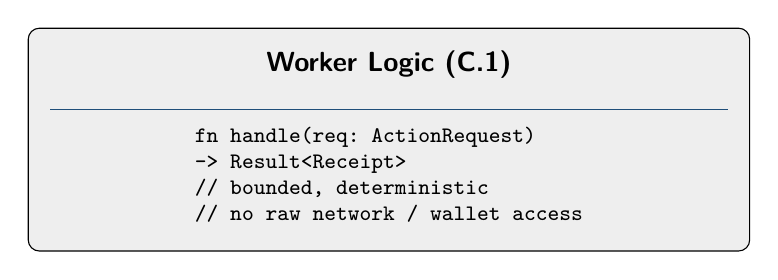
\begin{tikzpicture}[scale=1,transform shape,node distance=5mm and 10mm]
\node[draw,rounded corners,fill=ioibg,inner sep=8pt]{%
\begin{minipage}{86mm}
\centering{\sffamily\bfseries Worker Logic (C.1)}\par\vskip2pt
{\color{ioikw}\rule{\linewidth}{0.4pt}}\par\vskip4pt
{\ttfamily\footnotesize\begin{tabular}{@{}l@{}}
fn handle(req: ActionRequest)\\
-\textgreater{} Result\textless{}Receipt\textgreater{}\\
// bounded, deterministic\\
// no raw network / wallet access
\end{tabular}}
\end{minipage}};
\end{tikzpicture}
\end{center}
\emph{}

\hypertarget{c.2-the-policy-envelope-policy.json}{%
\subsection{\texorpdfstring{\textbf{C.2 The Policy Envelope
(policy.json)}}{C.2 The Policy Envelope (policy.json)}}\label{c.2-the-policy-envelope-policy.json}}

The firewall rules that govern the agent\textquotesingle s execution.
This ensures the agent cannot exfiltrate the user\textquotesingle s SSH
keys or drain their wallet.


\begin{center}
\needspace{6\baselineskip}
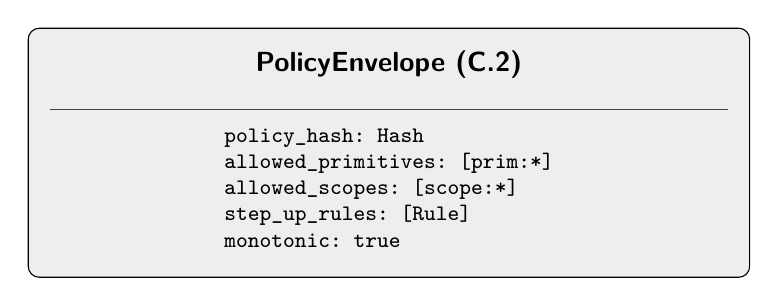
\begin{tikzpicture}[scale=1,transform shape,node distance=5mm and 10mm]
\node[draw,rounded corners,fill=ioibg,inner sep=8pt]{%
\begin{minipage}{86mm}
\centering{\sffamily\bfseries PolicyEnvelope (C.2)}\par\vskip2pt
{\color{ioikw}\rule{\linewidth}{0.4pt}}\par\vskip4pt
{\ttfamily\footnotesize\begin{tabular}{@{}l@{}}
policy\_hash: Hash\\
allowed\_primitives: [prim:*]\\
allowed\_scopes: [scope:*]\\
step\_up\_rules: [Rule]\\
monotonic: true
\end{tabular}}
\end{minipage}};
\end{tikzpicture}
\end{center}


\hypertarget{c.3-the-worker-manifest-manifest.json}{%
\subsection{\texorpdfstring{\textbf{C.3 The Worker Manifest
(manifest.json)}}{C.3 The Worker Manifest (manifest.json)}}\label{c.3-the-worker-manifest-manifest.json}}

The declarative manifest published to aiagent.xyz.

\textbf{\textbf{}}


\begin{center}
\needspace{6\baselineskip}
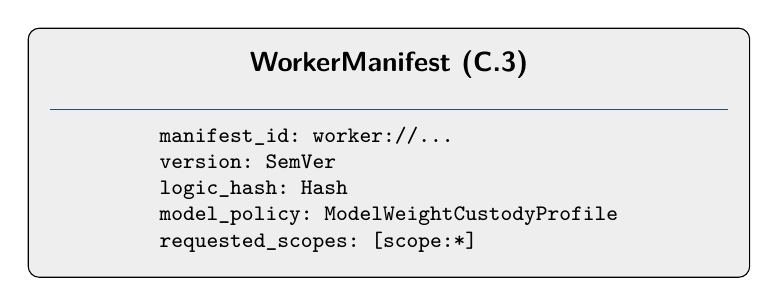
\begin{tikzpicture}[scale=1,transform shape,node distance=5mm and 10mm]
\node[draw,rounded corners,fill=ioibg,inner sep=8pt]{%
\begin{minipage}{86mm}
\centering{\sffamily\bfseries WorkerManifest (C.3)}\par\vskip2pt
{\color{ioikw}\rule{\linewidth}{0.4pt}}\par\vskip4pt
{\ttfamily\footnotesize\begin{tabular}{@{}l@{}}
manifest\_id: worker://...\\
version: SemVer\\
logic\_hash: Hash\\
model\_policy: ModelWeightCustodyProfile\\
requested\_scopes: [scope:*]
\end{tabular}}
\end{minipage}};
\end{tikzpicture}
\end{center}
\textbf{\textbf{}}

\hypertarget{c.4-normative-schema-connector-manifest}{%
\subsection{C.4 Illustrative Connector
Manifest}\label{c.4-normative-schema-connector-manifest}}

To ensure agents can be swapped between providers (avoiding vendor
lock-in), Connectors are defined by schema, not proprietary code.


\begin{center}
\needspace{6\baselineskip}
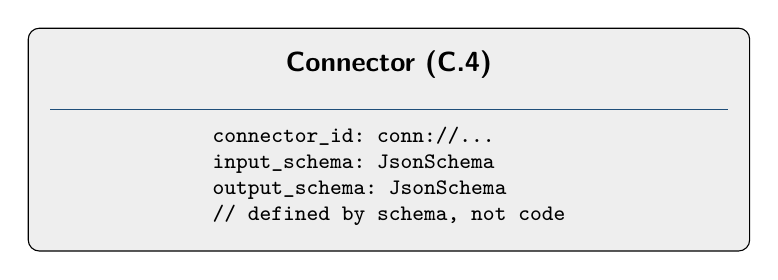
\begin{tikzpicture}[scale=1,transform shape,node distance=5mm and 10mm]
\node[draw,rounded corners,fill=ioibg,inner sep=8pt]{%
\begin{minipage}{86mm}
\centering{\sffamily\bfseries Connector (C.4)}\par\vskip2pt
{\color{ioikw}\rule{\linewidth}{0.4pt}}\par\vskip4pt
{\ttfamily\footnotesize\begin{tabular}{@{}l@{}}
connector\_id: conn://...\\
input\_schema: JsonSchema\\
output\_schema: JsonSchema\\
// defined by schema, not code
\end{tabular}}
\end{minipage}};
\end{tikzpicture}
\end{center}


\hypertarget{c.5-lifecycle-of-an-agentic-transaction-worked-example}{%
\subsection{C.5 Lifecycle of an Agentic Transaction (Worked
Example)}\label{c.5-lifecycle-of-an-agentic-transaction-worked-example}}

Linear flow of data transformation.

\hypertarget{appendix-d-claims-and-non-claims-the-scope-of-verification}{%
\section{Appendix D: Claims and Non-Claims (The Scope of
Verification)}\label{appendix-d-claims-and-non-claims-the-scope-of-verification}}

\begin{center}
\needspace{6\baselineskip}
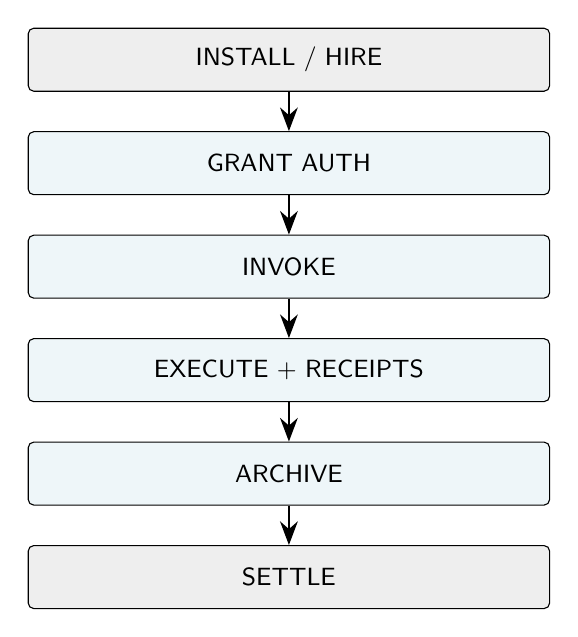
\begin{tikzpicture}[scale=1,transform shape,node distance=5mm and 10mm]
\node[ioiplain,text width=62mm] (h) {INSTALL / HIRE};
\node[ioibox,text width=62mm,below=of h] (g) {GRANT AUTH};
\draw[ioiflow] (h) --  (g);
\node[ioibox,text width=62mm,below=of g] (i) {INVOKE};
\draw[ioiflow] (g) --  (i);
\node[ioibox,text width=62mm,below=of i] (e) {EXECUTE + RECEIPTS};
\draw[ioiflow] (i) --  (e);
\node[ioibox,text width=62mm,below=of e] (a) {ARCHIVE};
\draw[ioiflow] (e) --  (a);
\node[ioiplain,text width=62mm,below=of a] (s) {SETTLE};
\draw[ioiflow] (a) --  (s);
\end{tikzpicture}
\end{center}

To provide absolute clarity to developers, cryptographers, legal
arbiters, and protocol auditors, the Hypervisor framework makes the
following explicit boundaries regarding its cryptographic proofs. The
protocol is designed around the philosophy of \textbf{Process Safety
over Model Safety}; therefore, we explicitly bound the scope of what is
mathematically guaranteed versus what is classified as heuristic or
non-binding telemetry.

\hypertarget{d.1-what-the-ioi-protocol-proves-normative-guarantees}{%
\subsection{D.1 What the IOI Protocol PROVES (Normative
Guarantees)}\label{d.1-what-the-ioi-protocol-proves-normative-guarantees}}

The proof carried by an IOI artifact is limited to the claims supported by
its cryptography, verifier, evidence source, and threat model. Given valid
implementations and the declared assumptions, an admitted receipt or proof
may establish:

The assurance state of the surrounding claim remains explicit: receipt or
attestation, evidence bundle, verification, acceptance, adjudication, and
settlement are distinct stages. Establishing one item below does not imply the
later stages unless the corresponding refs and governing contract establish
them.

\begin{enumerate}
\def\labelenumi{\arabic{enumi}.}
\tightlist
\item
  \textbf{Committed bytes and canonicalization:} The exact canonical bytes,
  identifiers, hashes, versions, and domain-separated commitments signed or
  included in the artifact.
\item
  \textbf{Declared policy and authority bindings:} Which policy hash,
  authority artifact, scope, approval, expiry, and revocation epoch were
  bound to the decision. A hash proves the binding, not faithful enforcement
  by unverified code or hardware.
\item
  \textbf{Signature and approval validity:} That the included signatures or
  approvals verify under the declared keys and algorithms and bind the shown
  request. This does not independently prove informed human understanding or
  legal consent.
\item
  \textbf{Ordering and inclusion:} That named receipts or events occur in a
  committed sequence, Merkle tree, operation log, state root, or bundle when
  the supplied inclusion and ordering proofs verify.
\item
  \textbf{Recorded execution-boundary result:} What the admitted runtime,
  adapter, provider, tool, sensor, actuator, or verifier reported, including
  success, denial, failure, observation, cost, and artifact refs. A signed
  report proves attribution to the signer, not the truth of every reported
  real-world fact.
\item
  \textbf{Verifier results:} That a named verifier accepted, rejected, or
  abstained on a claim under a declared version, input commitment, and
  assumption set. The verifier result is no broader than the verifier's
  specification and evidence coverage.
\item
  \textbf{Replay and state-root consistency:} That replay of the complete
  admitted operation and artifact set reproduces the stated projection or
  state root, when all required bytes and deterministic code are available.
\item
  \textbf{Specific proof-system or attestation claims:} A valid ZK, MPC,
  FHE, TEE, cTEE custody, timestamp, transparency-log, or external-evidence
  proof establishes only the exact statement specified by its profile and
  verifier under its stated assumptions.
\end{enumerate}

The architecture, product topology, openness of routing, correctness of a
model, safety of a physical act, legal consent, insurance coverage, and
faithful enforcement are not made true merely by placing their labels or
hashes inside a receipt.

\hypertarget{d.2-what-the-ioi-protocol-does-not-claim-non-claims}{%
\subsection{D.2 What the IOI Protocol DOES NOT CLAIM
(Non-Claims)}\label{d.2-what-the-ioi-protocol-does-not-claim-non-claims}}

To avoid the architectural traps of first-generation Decentralized AI
networks, IOI explicitly \textbf{does not} claim the following:

\begin{enumerate}
\def\labelenumi{\arabic{enumi}.}
\tightlist
\item
  \textbf{Bit-for-bit equivalence of foundational model inference:} IOI
  does not claim an LLM will output the exact same tokens when run on an
  Nvidia H100 versus an Apple M3 chip. IOI embraces floating-point drift
  at the heavy cognition layer. We claim only that the \textbf{Decision
  Verdict} rendered by the daemon effect boundary is fully
  deterministic. This is achieved via strict JCS normalization of
  \emph{ActionRequests} and, for sensitive egress cases, deterministic
  inspection profiles such as \emph{inspection\_v0} over local evidence
  graphs.
\item
  \textbf{Every local action is on-chain:} IOI does not claim, require,
  or desire that every local action, tool call, click, inference step,
  or filesystem access become a Mainnet transaction. The claim is
  narrower and stronger: any consequential boundary of Web4 Act must be
  transaction-shaped and capable of settlement or recourse when
  required.
\item
  \textbf{cTEE is not arbitrary full-speed private LLM inference on
  hostile-root consumer GPUs:} IOI does not claim to run full-parameter
  private LLM evaluations (e.g., Llama-3 70B) in plaintext on untrusted,
  consumer-grade rented GPUs without leakage. High-throughput execution
  uses Candidate-Lattice Private Decoding, where the model computes
  public weights to output structured token options while the
  private-head parameters are evaluated inside secure boundaries.
\item
  \textbf{cTEE does not protect plaintext proprietary model weights
  mounted on a hostile-root rented GPU:} if a developer mounts
  unencrypted model weights to a node where the provider holds host-root
  permissions, those weights are exposed. Protecting proprietary model
  IP requires a separate \textbf{ModelWeightCustodyProfile}: local or
  customer-controlled custody, provider API custody, accepted
  TEE/customer-cloud custody, cryptographic-operator partitioning, or an
  explicitly receipted provider-trust route. Private Workspace backed by
  cTEE protects workspace state; it does not by itself make proprietary
  weights safe on hostile-root hardware.
\item
  \textbf{A software-only cTEE sandbox does not protect plaintext
  proprietary weights in hostile-root GPU memory:} the IOI Hypervisor
  does not claim that a software-only cTEE protects proprietary weights
  loaded in plaintext into standard GPU memory on a hostile-root system.
  If a model owner mounts unencrypted weights on a remote machine
  without hardware confidential compute (TEEs) or cryptographic-operator
  partitioning, those weights can be dumped by the host administrator.
\item
  \textbf{Third-party model APIs are not a zero-knowledge or
  zero-disclosure path:} when a worker routes tool parameters or prompts
  to a proprietary remote API, those inputs cross the provider-trust
  boundary and are explicitly not a private execution pathway relative
  to that model provider.
\item
  \textbf{Measured boot / HypervisorOS is not a substitute for cTEE
  no-plaintext-custody or hardware confidential GPU protection:} proving
  that a node booted a valid, measured kernel image (via a
  \emph{HypervisorOSBootReceipt}) does not stop a physical host operator with a
  logic analyzer or malicious motherboard implants from capturing data
  in transit.
\item
  \textbf{Measured boot does not equal confidential computing:} measured
  boot proves \emph{what} software booted on the hardware; confidential
  computing (such as AMD SEV-SNP or Intel SGX) actively \emph{protects}
  running memory from unauthorized host observation. HypervisorOS relies
  on confidential hardware or cTEE software envelopes when weight
  secrecy is required.
\item
  \textbf{Universal Knowledge Optimality:} IOI does not prove that a
  worker used the best information available in the global universe. It
  proves only that the committed context slice, retrieval inputs, and
  evidence references were faithfully packaged and bound to the intent
  under the declared policy. If a superior source was never present in
  the worker's accessible memory/retrieval plane, retrieval corpus, or
  authorized context window, IOI cannot prove it should have been used.
\item
  \textbf{Wall-clock timestamps as consensus truth:} While the runtime
  records local \emph{SystemTime} for telemetry and debug activity
  streams (\emph{WorkloadReceiptEvent}), these are observational
  artifacts. IOI does not treat local wall-clock time as a
  Byzantine-fault-tolerant source of truth. All enforceable expiries and
  sequencing rely strictly on \textbf{Chain Time} or monotonic block
  heights.
\item
  \textbf{Semantic Correctness:} The protocol proves \textbf{Intent
  Compliance} (did the agent do what it said it would do within the
  rules?), not \textbf{Semantic Wisdom}. If a worker is authorized to
  spend \$50 and it buys a useless asset within that authorized scope,
  the protocol proves the spend was authorized and executed; it does not
  claim the worker made a "smart" decision. Web4 proves executable
  ownership and accountable consequence, not wisdom. Economic liability
  for an authorized but poor result, policy breach, provider failure, or
  developer defect is determined by the governing contract, evidence,
  jurisdiction, assurance posture, and claims process rather than a universal
  source-based rule in this whitepaper.
\item
  \textbf{Total On-Chain Duplication:} IOI does not claim that every
  state change or module invocation is duplicated on IOI L1. Hypervisor
  Node local settlement is designed to avoid public chain spam, storing
  operational and intermediate execution state locally within Agentgres.
\item
  \textbf{Monolithic Binaries:} IOI does not claim that the Hypervisor
  Node binary contains or owns model weights by default. Models are
  treated strictly as mounted cognition backends whose lifecycles are
  governed by independent deployment profiles.
\item
  \textbf{Hardware attestation as authority:} IOI does not claim that a
  TEE quote, secure enclave measurement, or confidential-compute
  attestation is sufficient to authorize an action. Hardware attestation
  may contribute evidence, but validity depends on the complete receipt
  set, policy hash, approval chain, capability scope, and settlement
  rules.
\item
  \textbf{Cryptographic compute as universal runtime:} IOI does not
  claim that FHE, MPC, ZK-ML, or proof VMs can currently replace all
  general-purpose agent execution. These substrates are strongest for
  bounded, typed, circuit-shaped, replayable, or privacy-sensitive
  subclaims. General browser automation, desktop operation, long-horizon
  mutable workflows, and open-ended agent behavior still require IOI's
  broader receipt and settlement boundary.
\item
  \textbf{Private-execution non-exposure as absolute secrecy:}
  Private-execution paths reduce disclosure under a declared threat model. They do
  not eliminate all side channels, implementation bugs, model leakage,
  misuse, or legal discovery risk. IOI's claim is narrower: the action's
  evidence posture, leakage bounds, and verifier requirements are
  explicit, auditable, and settlement-bound.
\item
  \textbf{Global AI alignment:} IOI does not claim to solve global AI
  alignment or inner alignment within neural networks. The protocol is
  strictly an execution-boundary containment system; it bounds the
  consequential effects of machine authority, and does not legislate the
  values, training data, or internal goals of any model.
\item
  \textbf{Raw model output as authoritative:} IOI does not claim that
  raw model output is legally or economically authoritative by itself.
  Authority attaches to the canonical ActionRequest, policy hash,
  approval chain, capability scope, and receipt set that wrap the
  output, not to the output as such. A receipt does not prove the
  underlying model was wise, truthful, or globally optimal.
\item
  \textbf{Agentgres as universal store:} Agentgres is not a universal
  replacement for OLAP engines, vector databases, blob stores, local UI
  state, generic event logs, or IOI L1 settlement.
\item
  \textbf{SQL writes bypassing operation settlement:} Agentgres does not
  allow arbitrary SQL writes to bypass operation settlement. The
  Postgres bridge serves projection reads; canonical writes must compile
  into Agentgres operations.
\item
  \textbf{Sealed archive as authority:} A sealed archive does not prove
  restore authority by existing. A blob CID is not canonical runtime
  truth by itself; Agentgres records the archive meaning, policy/authority
  refs, state root, and restore receipts, while applicable authority
  providers decide who may restore.
\item
  \textbf{Omnipresent control over opaque runtimes:} The IOI Authority
  Gateway does not claim to have direct, internal visibility into the
  state machines of closed-source, remote, or compiled third-party agent
  systems. Instead, it mediates only the control points an adapter can
  observe and can record proposals, decisions, observations, and receipts at
  those points. It cannot prove that opaque effects outside those hooks were
  intercepted or did not occur.
\item
  \textbf{Static encryption-at-rest as no-plaintext-custody:} static
  ``encryption-at-rest'' is not a substitute for dynamic
  no-plaintext-custody. If a node retains plaintext custody of data in
  memory during execution, its state is compromised on a hostile-root
  machine.
\item
  \textbf{Storage backends owning artifact meaning:} storage backends
  (such as Filecoin, IPFS, S3, or local disk) do not own or understand
  artifact meaning. They are passive byte repositories; meaning is owned
  exclusively by the Agentgres Artifact Plane via \emph{ArtifactRefs}
  and receipt linkages.
\item
  \textbf{Fuzzy memory as the complete cognition substrate:} neither the
  Agent Wiki (\emph{ioi-memory}) nor Agentgres is the complete cognition
  substrate of the worker. Fuzzy, volatile context resides in the
  semantic memory plane and crosses the Agentgres admission boundary via
  \emph{ContextMutation} commits only when state must be rendered
  durable and portable.
\item
  \textbf{Reversibility of embodied action:} physical robotics and
  embodied actions cannot be ``undone'' or rolled back like local
  database rows. They require first-class physical safety primitives,
  including a defined \emph{SafetyEnvelope}, a
  \emph{PhysicalActionPolicy}, and an override-capable
  \emph{EmergencyStopAuthority}.
\item
  \textbf{Participant consensus as truth or authority:} an OutcomeRoom board,
  chat, vote, leaderboard, repeated model answer, or participant consensus is
  an evidence input and projection. It does not admit a CollaborativeWorkGraph
  mutation, widen authority, promote memory or ontology state, or establish
  correctness without the declared hosted or federated admission and verifier
  path.
\item
  \textbf{One global collaboration or ontology database:} AIIP and
  OutcomeRooms do not merge sovereign Agentgres domains into one mutable graph.
  Federated ontologies preserve local canonicality, namespace, version,
  mappings, uncertainty, contradiction, and policy-bound views. The shared
  room state always names a hosted admission domain or versioned federated
  admission policy.
\item
  \textbf{Multiplicity as independence:} multiple models, Workers, runtime
  nodes, clouds, providers, or keys controlled by one principal are not
  independent parties merely because they are numerous. Multi-party claims
  require disclosed affiliations and separate accountable control over
  authority, revocation, truth, risk, verification, challenge, or settlement.
\item
  \textbf{Environment recovery as outcome recovery:} restoring a VM, channel,
  workspace, Worker, or provider session does not prove that an external API,
  payment, message, deployment, or physical action did or did not commit.
  Consequential effects declare \texttt{replayable},
  \texttt{checkpointable}, \texttt{compensatable},
  \texttt{reconciliation\_required}, or \texttt{non\_retryable}; ambiguous
  effects are reconciled before retry, and compensation is separately
  authorized and receipted.
\item
  \textbf{Daemon admission as authority:} the daemon admits and enforces work
  and mediates or executes effects, but it does not self-grant portable,
  secret-bearing, spend-bearing, declassification, cross-domain, or high-risk
  power. Local/domain policy and the applicable authority provider authorize;
  Agentgres admits resulting durable operational truth.
\end{enumerate}

The Physics-to-Digital Evidence Loop (Target Embodied Runtime)

IOI cannot rewrite physical laws and does not claim to make the material
world cryptographically reversible. The speculative Embodied Runtime target
binds PhysicalActionIntent, safety-policy refs, authority refs, sensor
evidence, command hashes, adapter/controller identity, results, telemetry,
incidents, and recovery state through receipts and Agentgres admission. Those
records support audit and verification under their capture and trust
assumptions; they do not independently prove that a physical condition was
safe or that motion occurred faithfully. Local safety controllers and
hardware interlocks retain the real-time veto. Any future escrow, liability,
or dispute consequence must come from an implemented governing contract and
verified evidence, not an automatic rule in this whitepaper.

\hypertarget{d.3-benchmark-and-routing-non-claims}{%
\subsection{D.3 Benchmark and Routing
Non-Claims}\label{d.3-benchmark-and-routing-non-claims}}

IOI \emph{BenchmarkReceipts} record a benchmark execution and verifier
result under a declared profile, environment, rubric, evidence set, and
worker manifest. They support the scoped benchmark claim under those
assumptions; they do not prove universal intelligence, universal optimality,
or permanent superiority across all future tasks.

MoW routing receipts record that a worker was selected from a declared
candidate set under a named routing policy and decision material. They do not
prove that the policy was faithfully implemented without applicable
conformance evidence or that the selected worker is globally best. They make
the declared decision inspectable and challengeable.

Sparse Worker Categories are relative labor markets, not universal
intelligence rankings.

\hypertarget{appendix-e-fail-closed-verdict-logic}{%
\section{Appendix E: Fail-Closed Verdict
Logic}\label{appendix-e-fail-closed-verdict-logic}}

This appendix summarizes the normative conformance contracts for
Hypervisor Core, the Hypervisor Daemon, and compatible harness profile
adapters. To guarantee that autonomous systems cannot bypass safety
constraints, the runtime must enforce the \textbf{Intent Resolution
Contract} (CIRC), the \textbf{Effect Execution Contract} (CEC), and the
\textbf{Harness Profile Adapter Conformance} boundary for third-party
harnesses, model runtimes, worker profiles, and module executors.

These rules dictate the ``Fail-Closed'' behavior of the Hypervisor
Core and daemon effect boundary. They enforce a ``Zero Heuristics / Zero Hidden Fallbacks''
doctrine: zero ad hoc, topic-specific, provider-shortcut, or hidden-fallback
heuristics that bypass typed intent resolution, plus zero unreceipted effect
retries hidden inside one admitted operation. Generic deterministic
heuristics remain allowed when they are feature-based, cross-domain,
task-class-aware, explainable, and policy-controlled. They are the conformance
rules that prevent Act from degrading into Web2 automation: if intent
cannot acquire transaction shape, it cannot become sovereign
consequence.

\hypertarget{e.1-intent-resolution-contract-circ}{%
\subsection{E.1 Intent Resolution Contract
(CIRC)}\label{e.1-intent-resolution-contract-circ}}

\textbf{CIRC governs the pre-execution phase. It is the }\emph{semantic
collapse}\textbf{ contract. It ensures that probabilistic inference
(e.g., embedding searches, LLM intent parsing) collapses into one
deterministic, replayable route decision or an explicit abstention.}

To pass the CIRC gate, the Hypervisor Daemon MUST enforce the following
invariants:

\begin{enumerate}
\def\labelenumi{\arabic{enumi}.}
\item
  \textbf{The Three-Layer Rule:} The resolver MUST enforce distinct
  layers:

  \begin{enumerate}
  \def\labelenumii{\arabic{enumii}.}
  \tightlist
  \item
    \emph{Intent}: Domain-level semantics (what the user wants).
  \item
    \emph{Capability}: Primitive execution boundaries (\emph{prim:*},
    what is physically possible and isolated).
  \item
    \emph{Tool}: Concrete implementation mechanism (how the action is
    executed).
  \item
    \emph{Fail-Closed Action:} If a tool tries to bypass semantic
    ranking or if capabilities encode domain logic (e.g.,
    \emph{prim:math.eval} instead of \emph{prim:sys.exec}), the runtime
    MUST reject the configuration with \emph{OntologyViolation}.
  \end{enumerate}
\item
  \textbf{The Structural Retrieval Rule:} Retrieval affordances MUST
  describe structural evidence shapes (e.g., \emph{queryable\_index},
  \emph{timestamped\_record}), not domain semantics or provider families
  (e.g., \emph{google\_news}).

  \begin{enumerate}
  \def\labelenumii{\arabic{enumii}.}
  \tightlist
  \item
    \emph{Fail-Closed Action:} If query inference directly emits
    provider IDs, hostnames, or pre-designated query-class switchboards
    instead of typed retrieval requirements, the runtime MUST abort with
    \emph{ResolverContractViolation}.
  \end{enumerate}
\item
  \textbf{Feasibility \& Hard Constraints:} Feasibility MUST be
  determined strictly upfront. Trial-and-error routing is forbidden. The
  resolver MUST verify that all required \emph{prim:*} capabilities are
  satisfiable by the active tools, and that applicable authority and policy
  do not prohibit execution.

  \begin{enumerate}
  \def\labelenumii{\arabic{enumii}.}
  \tightlist
  \item
    \emph{Fail-Closed Action:} If the top-ranked intent is infeasible,
    selection MUST proceed in ranked order to the next feasible intent.
    Only when no admissible candidate remains may the resolver emit a typed
    infeasible, blocked, ambiguous, or abstention state. It MUST NOT
    short-circuit to a tool before deterministic intent winner selection.
  \end{enumerate}
\end{enumerate}

\hypertarget{e.2-effect-execution-contract-cec}{%
\subsection{E.2 Effect Execution Contract
(CEC)}\label{e.2-effect-execution-contract-cec}}

\textbf{CEC governs the post-resolution execution discipline. It is the
}\emph{effect collapse}\textbf{ contract. CEC takes the already-resolved
intent and governs payload synthesis, execution, and verification. It
permits probabilistic synthesis }\emph{prior}\textbf{ to execution,
while strictly enforcing an admitted-effect boundary }\emph{during}\textbf{
execution. Hidden retries inside that admitted effect are forbidden;
governed remediation opens a new ActionProposal, gate, receipt, and
observation path.}

The Hypervisor Daemon MUST enforce the CEC Execution State Machine:

\begin{enumerate}
\def\labelenumi{\arabic{enumi}.}
\item
  \emph{contract\_loaded} \& \emph{discovery}: The runtime gathers
  ground-truth host topology and provider candidates based on typed
  discovery.
\item
  \emph{provider\_selection} / \emph{payload\_synthesis} \textbf{(The
  Safe Sandbox):} Probabilistically generating, linting, dry-running,
  and iteratively refining the execution payload is explicitly permitted
  and encouraged \emph{within this state only}.
\item
  \emph{execution} \textbf{(The Admitted-Effect Boundary):} Once the
  payload transitions to execution, that admitted effect is committed.
  It MUST be one deterministic effect attempt under the current receipt
  chain.

  \begin{enumerate}
  \def\labelenumii{\arabic{enumii}.}
  \tightlist
  \item
    \emph{Fail-Closed Action:} Post-execution heuristic retries using
    the real environment as a sandbox (unbounded ``try-and-catch''
    code-rewriting loops) are strictly forbidden inside the same
    admitted effect. If execution fails, it MUST emit
    \emph{ExecutionFailedTerminal}, \emph{partial}, \emph{blocked}, or
    \emph{unverified}. A repair attempt must begin as a new proposal with
    new gate and receipt material.
  \end{enumerate}
\item
  \emph{verification}: The runtime MUST verify read-state evidence with
  a cryptographic commit. It MUST NOT assume success from process exit
  status alone.
\item
  \emph{completion\_gate} \& \emph{terminal}: The final gate before
  integration.
\end{enumerate}

To pass the CEC Completion Gate, the Hypervisor Daemon MUST enforce the
following:

\begin{enumerate}
\def\labelenumi{\arabic{enumi}.}
\item
  \textbf{The Judge Integrity Rule:} Runtime success adjudication MUST
  be receipt-driven. Final chat reply text or debug strings MUST NOT be
  the primary evidence channel for pass/fail. Completion gates MUST rely
  on typed receipt fields (e.g., \emph{contract\_version},
  \emph{satisfied}, \emph{evidence\_commit\_hash}).
\item
  \textbf{Receipt Completeness Invariant:} Every governed execution MUST
  emit machine-readable evidence records matching its
  \emph{applicability\_class} (e.g., \emph{topology\_dependent},
  \emph{deterministic\_local}, \emph{remote\_retrieval}).

  \begin{enumerate}
  \def\labelenumii{\arabic{enumii}.}
  \tightlist
  \item
    \emph{Fail-Closed Action:} If any required receipt is missing, any
    required postcondition is missing, or verification fails, the
    runtime MUST emit \emph{ERROR\_CLASS=\allowbreak{}Execution\allowbreak{}Contract\allowbreak{}Violation} and
    block the \emph{agent\_\_complete} status.
  \end{enumerate}
\end{enumerate}

\hypertarget{e.3-harness-profile-adapter-conformance}{%
\subsection{E.3 Harness Profile Adapter
Conformance}\label{e.3-harness-profile-adapter-conformance}}

Hypervisor may route work through Codex-style coding agents, Claude
Code-style CLIs, DeepSeek-style harnesses, OpenHands/Aider-style local
tools, hosted workers, Rust/WASM modules, service engines, and custom
enterprise harnesses. These systems are useful execution participants,
but they are not authority roots and not completion truth.

Every HarnessProfile Adapter must publish a descriptor declaring its
primitive capabilities, authority-scope requirements, supported receipts,
state projection rules, secret-handling posture, cTEE compatibility, and
replay support. It must map harness-native events into Hypervisor
objects: resolver receipts, ActionProposals, GateResults,
ExecutionResults, NormalizedObservations, ArtifactRefs/PayloadRefs, and
terminal receipt candidates. It must not hold wallet.network root
secrets, mint \emph{scope:*} grants, widen policy, bypass step-up, treat
harness-native approval prompts as wallet.network approvals, or treat
harness memory as Agentgres truth.

This adapter rule is what allows IOI to benefit from a growing ecosystem
of open-source and proprietary harnesses without making any one harness
the protocol substrate.

\hypertarget{e.4-the-anti-heuristic-doctrine}{%
\subsection{E.4 The Anti-Heuristic
Doctrine}\label{e.4-the-anti-heuristic-doctrine}}

In the IOI architecture, ambiguity equals failure. There are no ``best
effort'' policy bypasses or ``heuristic'' state merges.

Implementations MUST NOT:

\begin{enumerate}
\def\labelenumi{\arabic{enumi}.}
\tightlist
\item
  Use predesignated query archetypes or domain buckets as a stand-in for
  typed provider discovery.
\item
  Gate success primarily on reply text or substring matches over debug
  output.
\item
  Route back to payload synthesis for a heuristic retry after a
  verification failure at the completion gate.
\end{enumerate}

\textbf{This Fail-Closed Verdict Logic is the bedrock of the Determinism
Boundary. It means that while an agent's }\emph{thoughts}\textbf{ and
}\emph{synthesis}\textbf{ may be probabilistic and creative, its admitted
}\emph{consequences}\textbf{ must cross a mathematically bound,
receipt-backed, policy-explainable effect boundary. Insurability and
legal recourse depend on the declared contract, jurisdiction, and
receipt class rather than on raw model output.}

Internet of Intelligence Protocol • Whitepaper v1.8.0 • © 2026 IOI
Foundation

\hypertarget{appendix-f-references-normative-standards}{%
\section{Appendix F: References \& Normative
Standards}\label{appendix-f-references-normative-standards}}

This section details the normative specifications, cryptographic
standards, and academic literature that form the foundational
assumptions of the IOI Protocol.

\hypertarget{f.1-normative-ietf-web-standards}{%
\subsection{F.1 Normative IETF \& Web
Standards}\label{f.1-normative-ietf-web-standards}}

These standards govern the deterministic formulation of intents, payload
serialization, and network routing within the Hypervisor Daemon and IOI
L0/domain substrate.

\begin{itemize}
\tightlist
\item
  \textbf{{[}RFC 8785{]}} Rundgren, A., Harrison, R., \& Sporny, C.
  (2020). \emph{JSON Canonicalization Scheme (JCS).} Internet
  Engineering Task Force (IETF). Defines the strict canonicalization
  required to prevent hash malleability in JSON payloads (used
  throughout the IOI Determinism Boundary).
\item
  \textbf{{[}RFC 3986{]}} Berners-Lee, T., Fielding, R., \& Masinter, L.
  (2005). \emph{Uniform Resource Identifier (URI): Generic Syntax.}
  IETF. Defines the parsing and resolution structure adapted for the
  \emph{ai://} identifier grammar used by the Inter-Autonomous-System
  Protocol (AIIP).
\item
  \textbf{{[}RFC 5234{]}} Crocker, D., \& Overell, P. (2008).
  \emph{Augmented BNF for Syntax Specifications: ABNF.} IETF. Defines
  the grammar for parsing the AIIP namespace.
\item
  \textbf{{[}RFC 8949{]}} Bormann, C., \& Hoffman, P. (2020).
  \emph{Concise Binary Object Representation (CBOR).} IETF. An available
  versioned binary encoding for owner contracts that select it; this
  whitepaper does not mandate a universal offload or session-packet format.
\item
  \textbf{{[}RFC 3161{]}} Adams, C., Cain, P., Pinkas, D., \&
  Zuccherato, R. (2001). \emph{Internet X.509 Public Key Infrastructure
  Time-Stamp Protocol (TSP).} IETF. Referenced for off-chain anchor
  validity.
\end{itemize}

\hypertarget{f.2-cryptographic-standards-post-quantum-classical}{%
\subsection{F.2 Cryptographic Standards (Post-Quantum \&
Classical)}\label{f.2-cryptographic-standards-post-quantum-classical}}

The protocol's Strict Hybrid Cryptography model relies on the following
National Institute of Standards and Technology (NIST) and industry
specifications.

\begin{itemize}
\tightlist
\item
  \textbf{{[}FIPS 202{]}} National Institute of Standards and
  Technology. (2015). \emph{SHA-3 Standard: Permutation-Based Hash and
  Extendable-Output Functions.} Defines the SHAKE-256 algorithm targeted
  for Post-Quantum artifact hashing.
\item
  \textbf{{[}FIPS 203{]}} National Institute of Standards and
  Technology. (2024). \emph{Module-Lattice-Based Key-Encapsulation
  Mechanism Standard.} Defines the ML-KEM family, which a reviewed
  versioned hybrid transport profile may select with explicit parameters.
\item
  \textbf{{[}FIPS 204{]}} National Institute of Standards and
  Technology. (2024). \emph{Module-Lattice-Based Digital Signature
  Standard.} Defines the ML-DSA family, which a reviewed versioned
  authority or commitment profile may select.
\item
  \textbf{{[}RFC 8032{]}} Josefsson, S., \& Liusvaara, I. (2017).
  \emph{Edwards-Curve Digital Signature Algorithm (EdDSA).} IETF.
  Defines EdDSA, an available classical signature family for profiles that
  select it. No genesis or wallet suite is selected in this whitepaper.
\item
  \textbf{{[}BLAKE3{]}} O\textquotesingle Connor, J., Aumasson, J. P.,
  Neves, S., \& Wilcox-O\textquotesingle Hearn, Z. (2020). \emph{BLAKE3:
  one function, fast everywhere.} A candidate high-throughput hash for
  owner profiles; not a protocol-wide fixed choice here.
\end{itemize}

\hypertarget{f.3-consensus-distributed-systems}{%
\subsection{F.3 Consensus \& Distributed
Systems}\label{f.3-consensus-distributed-systems}}

The challenge-dominant settlement research candidate in Section 5.3 draws on
the following BFT and distributed-systems research. These references do not
constitute a selected IOI L1 consensus engine.

\begin{itemize}
\tightlist
\item
  \textbf{{[}PBFT{]}} Castro, M., \& Liskov, B. (1999). \emph{Practical
  Byzantine Fault Tolerance. }Proceedings of the Third Symposium on
  Operating Systems Design and Implementation (OSDI). The foundational
  baseline for BFT mesh assumptions.
\item
  \textbf{{[}HotStuff{]}} Yin, M., Malkhi, D., Reiter, M. K., Gueta, G.
  G., \& Abraham, I. (2019). \emph{HotStuff: BFT Consensus with
  Linearity and Responsiveness.} Proceedings of the ACM Symposium on
  Principles of Distributed Computing (PODC). Serves as the structural
  background for possible linear-view research profiles.
\item
  \textbf{{[}MinBFT{]}} Veronese, G. S., Correia, M., Bessani, A. N., \&
  Lung, L. C. (2011). \emph{Efficient Byzantine Fault-Tolerance.} IEEE
  Transactions on Computers. Provides the mathematical proofs that
  hardware-backed monotonic counters can reduce equivocation, enabling
  more efficient Byzantine fault-tolerant replication under the paper's
  stated assumptions.
\end{itemize}

\hypertarget{f.4-artificial-intelligence-infrastructure}{%
\subsection{F.4 Artificial Intelligence \&
Infrastructure}\label{f.4-artificial-intelligence-infrastructure}}

Protocols and algorithms supporting the cognitive and operational
capabilities of the IOI architecture.

\begin{itemize}
\tightlist
\item
  \textbf{{[}MCP{]}} Anthropic. (2024). \emph{Model Context Protocol
  Specification.} The standard open integration protocol utilized by the
  IOI Authority Gateway to securely expose and mediate host tools to
  external agent harnesses.
\item
  \textbf{{[}ERC-4337{]}} Buterin, V., et al. (2021). \emph{Account
  Abstraction Using Alt Mempool.} Ethereum Improvement Proposals. The
  structural target for the Agent Execution Account managed by
  wallet.network policy and authority grants.
\item
  \textbf{{[}MoE{]}} Shazeer, N., et al. (2017). \emph{Outrageously
  Large Neural Networks: The Sparsely-Gated Mixture-of-Experts Layer.}
  Referenced as the model-routing analogue for IOI's execution-layer
  Mixture of Workers concept.
\end{itemize}

\hypertarget{f.5-commercial-model-supply-boundary}{%
\subsection{F.5 Commercial Model-Supply Boundary (Non-Normative Procurement
Evidence)}\label{f.5-commercial-model-supply-boundary}}

The following provider materials were reviewed on July 11, 2026. They explain
the commercial boundary motivating \emph{ModelRouteRightsContract}; they are
dated procurement evidence, not permanent protocol law. Runtime admission
must resolve the current terms, order form, model-specific terms, and signed
agreement rather than relying on this snapshot.

\begin{itemize}
\tightlist
\item
  \textbf{{[}OpenAI Services Agreement{]}} OpenAI. (effective January 1,
  2026). \href{https://openai.com/policies/services-agreement/}{OpenAI
  Services Agreement}. Distinguishes licensed business/API use, individual
  end-user accounts, credential sharing restrictions, customer applications,
  and usage-based services.
\item
  \textbf{{[}OpenAI Subscription/API Separation{]}} OpenAI Help Center.
  \href{https://help.openai.com/en/articles/8156019}{How can I move my
  ChatGPT subscription to the API?}. States that ChatGPT subscription and API
  billing are separately managed.
\item
  \textbf{{[}Anthropic Subscription/API Separation{]}} Anthropic Help
  Center. (March 16, 2026).
  \href{https://support.claude.com/en/articles/9876003-i-have-a-paid-claude-subscription-pro-max-team-or-enterprise-plans-why-do-i-have-to-pay-separately-to-use-the-claude-api-and-console}{Paid
  Claude plans and API/Console separation}. Distinguishes interactive paid
  plans from separately provisioned developer API access.
\item
  \textbf{{[}OpenRouter Terms and Routing{]}} OpenRouter. (terms updated
  July 6, 2026). \href{https://openrouter.ai/terms/}{Terms of Service} and
  \href{https://openrouter.ai/docs/guides/routing/provider-selection}{Provider
  Routing}. Establish that aggregator access remains subject to applicable
  model terms, provider/data-policy selection, fallback behavior, and resale
  restrictions.
\end{itemize}

\end{document}
